\documentclass[
    fontsize=10pt,
    a4paper,
    twoside=false,
    parskip=false,
]{kaobook}

\usepackage{polyglossia} % Локализация документа --- переносы и всё такое
\setmainlanguage{russian}
\setotherlanguage{english}

\usepackage[autostyle]{csquotes} % Правильные кавычки в зависимости от языка

\usepackage{xurl} % Разрешить переносить URL на любой букве
\usepackage[noheader]{gitver}
\usepackage{caption}
\usepackage{subcaption}

\NewDocumentCommand{\email}{m}{\href{mailto:#1}{#1}} % Кликабельный email

%% : с чуть более узки расстоянием по бокам.
%% Определено в pseudo, потому пока что закомментировано
 \NewDocumentCommand \rng { } {
 \nolinebreak
 \mathinner { : }
 \nolinebreak
 }

\usepackage{tikz}
\usetikzlibrary{arrows.meta}
\usetikzlibrary{external}
\usetikzlibrary{positioning}
\usetikzlibrary{shapes.geometric}
\usetikzlibrary{automata}
\usetikzlibrary{decorations.pathmorphing}
\usetikzlibrary{backgrounds}
\usetikzlibrary{calc}
\usetikzlibrary{arrows}
\usetikzlibrary{fit}


\tikzsetexternalprefix{figures/externalized/}

% Required in RegularLanguages
\tikzset{snake it/.style={decorate, decoration=snake}}
\tikzset{
    side by side/.style 2 args={
            line width=2pt,
            #1,
            postaction={
                    clip,postaction={draw,#2}
                }
        }
}

% \usetikzlibrary{fit, calc}

\usepackage{amsthm}
\usepackage{nicematrix}

% \setmathfont[range={\doubleplus}, Scale=MatchLowercase]{Asana Math}
\NewDocumentCommand{\derives}{O{*}}{\xRightarrow[]{#1}}


\usepackage{thmtools}

%%% theorem-like envs
\theoremstyle{definition}

\declaretheoremstyle[spaceabove=0.5\topsep,
    spacebelow=0.5\topsep,
    headfont=\bfseries\sffamily,
    bodyfont=\normalfont,
    headpunct=.,
    postheadspace=5pt plus 1pt minus 1pt]{myStyle}
\declaretheoremstyle[spacebelow=\topsep,
    headfont=\bfseries\sffamily,
    bodyfont=\normalfont,
    headpunct=.,
    postheadspace=5pt plus 1pt minus 1pt,]{myStyleWithFrame}
\declaretheoremstyle[spacebelow=\topsep,
    headfont=\itshape\sffamily,
    bodyfont=\normalfont,
    headpunct=.,
    postheadspace=5pt plus 1pt minus 1pt,
    qed=\blacksquare]{myProofStyleWithFrame}

\tcbuselibrary{breakable, skins}
\tcbset{shield externalize}
\tcbset{boxrule=0pt,
    sharp corners,
    borderline west={0.3mm}{0pt}{black},
    frame hidden,
    enhanced,
    interior hidden,
    left=2mm,
    top = 1mm,
    bottom = 1mm,
    right = 0.5mm
}

\tcolorboxenvironment{theorem}{}
% \tcolorboxenvironment{theorem*}{}
% \tcolorboxenvironment{axiom}{}
% \tcolorboxenvironment{assertion}{}
\tcolorboxenvironment{lemma}{}
% \tcolorboxenvironment{proposition}{}
% \tcolorboxenvironment{corollary}{}
\tcolorboxenvironment{definition}{}
% \tcolorboxenvironment{proofReplace}{toprule=0mm,bottomrule=0mm,rightrule=0mm, colback=white, breakable }

\declaretheorem[name=Теорема, numberwithin=chapter, style=myStyleWithFrame]{theorem}
% \declaretheorem[name=Теорема, numbered=no, style=myStyleWithFrame]{theorem*}
% \declaretheorem[name=Аксиома, sibling=theorem, style=myStyleWithFrame]{axiom}
% \declaretheorem[name=Преположение, sibling=theorem, style=myStyleWithFrame]{assertion}
\declaretheorem[name=Лемма, sibling=theorem, style=myStyleWithFrame]{lemma}
% \declaretheorem[name=Предложение, sibling=theorem, style=myStyleWithFrame]{proposition}
% \declaretheorem[name=Следствие, numberwithin=theorem, style=myStyleWithFrame]{corollary}

\declaretheorem[name=Определение, numberwithin=chapter, style=myStyleWithFrame]{definition}
% \declaretheorem[name=Свойство, numberwithin=chapter, style=myStyle]{property}
% \declaretheorem[name=Свойства, numbered=no, style=myStyle]{propertylist}

\declaretheorem[name=Пример, numberwithin=chapter, style=myStyle]{example}
\declaretheorem[name=Замечание, numbered=no, style=myStyle]{remark}

\declaretheorem[name=Доказательство, numbered=no, style=myProofStyleWithFrame]{proofReplace}
\renewenvironment{proof}[1][\proofname]{\begin{proofReplace}}{\end{proofReplace}}
% \declaretheorem[name=Доказательство, numbered=no, style=myProofStyleWithFrame]{longProof}

\declaretheorem[name={Набросок доказательства}, numbered=no, style=myProofStyleWithFrame]{proofSketch}

\usepackage[linesnumbered,algochapter,lined,noend]{algorithm2e}

\renewcommand*{\algorithmcfname}{Алгоритм}
\SetKwInput{KwData}{Входные данные}
\SetKwInput{KwResult}{Результат работы}


\usepackage{kaobiblio} % Обертка для biblatex, позволяет печатать сноску сбоку
\addbibresource{FormalLanguageConstrainedReachabilityLectureNotes.bib}

\newcommand*\circled[1]{\tikz[baseline=(char.base)]{
            \node[shape=circle,draw,inner sep=2pt] (char) {#1};}}

\pghyphenation[]{russian}{%
тео-ре-ти-ко-мно-жест-вен-ных
}

\tikzexternalize

\title{О достижимости с ограничениями в терминах формальных языков}
\author{Семён Григорьев}
\date{\gitVer{}}

\begin{document}

\frontmatter

\maketitle
\tableofcontents

\addchap{Список авторов}

\begin{description}[style=nextline]
      \item[Семён Григорьев]
            Санкт-Петербургский государственный университет, Университетская набережная, 7/9, Санкт-Петербург, 199034, Россия \\
            \email{s.v.grigoriev@spbu.ru}\\
            JetBrains Research, Приморский проспект 68-70, здание 1, Санкт-Петербург, 197374, Россия \\
            \email{semyon.grigorev@jetbrains.com}
      \item[Екатерина Вербицкая]
            JetBrains Research, Приморский проспект 68-70, здание 1, Санкт-Петербург, 197374, Россия \\
            \email{ekaterina.verbitskaya@jetbrains.com}
      \item[Дмитрий Кутленков]
            Санкт-Петербургский государственный университет, Университетская набережная, 7/9, Санкт-Петербург, 199034, Россия \\
            \email{kutlenkov.dmitri@gmail.com}
      \item[]
\end{description}

Полный список людей, внёсших свой вклад в данную работу, можно посмотреть на страничке проекта:
\url{https://github.com/FormalLanguageConstrainedPathQuerying/FormalLanguageConstrainedReachability-LectureNotes}


\mainmatter
\setchapterstyle{kao}

\addchap{Введение}
\tikzsetfigurename{Introduction_}

Теория формальных языков находит применение не только в ставших уже классическими задачах синтаксического анализа кода (языков программирования, искусственных языков) и естественных языков, но и в других областях, таких как статический анализ кода, графовые базы данных, биоинформатика, машинное обучение.

Например, в машинном обучении использование формальных грамматик позволяет передать искусственной генеративной нейронной сети, предназначенной для построения цепочек с определёнными свойствами, знания о синтаксической структуре этих цепочек, что позволяет существенно упростить процесс обучения и повысить качество результата~\sidecite{10.5555/3305381.3305582}.
Вместе с этим, развиваются подходы, позволяющие нейронным сетям наоборот извлекать синтаксическую структуру (строить дерево вывода) для входных цепочек~\sidecite{kasai-etal-2017-tag,kasai-etal-2018-end}.

В биоинформатике формальные грамматики нашли широкое применение для описания особенностей вторичной структуры геномных и белковых последовательностей~\sidecite{Dyrka2019,WJAnderson2012,zier2013rna}.
Соответствующие алгоритмы синтаксического анализа используются при создании инструментов обработки данных.

Таким образом, теория формальных языков выступает в качестве основы для многих прикладных областей, а алгоритмы синтаксического анализа применимы не только для обработки естественных языков или языков программирования.
Нас же в данной работе будет интересовать применение теории формальных языков и алгоритмов синтаксического анализа для анализа графовых баз данных и для статического анализа кода.

Одна из классических задач, связанных с анализом графов~--- это поиск путей в графе.
Возможны различные формулировки этой задачи.
В некоторых случаях необходимо выяснить, существует ли путь с определёнными свойствами между двумя выбранными вершинами.
В других же ситуациях необходимо найти все пути в графе, удовлетворяющие некоторым свойствам или ограничениям.
Например, в качестве ограничений можно указать, что искомый путь должен быть простым, кратчайшим, гамильтоновым и так далее.

Один из способов задавать ограничения на пути в графе основан на использовании формальных языков.
Базовое определение языка говорит нам, что язык~--- это множество слов над некоторым алфавитом.
Если рассмотреть граф, рёбра которого помечены символами из алфавита, то путь в таком графе будет задавать слово: достаточно соединить последовательно символы, лежащие на рёбрах пути.
Множество же таких путей будет задавать множество слов или язык.
Таким образом, если мы хотим найти некоторое множество путей в графе, то в качестве ограничения можно описать язык, который должно задавать это множество.
Иными словами, задача поиска путей может быть сформулирована следующим образом: необходимо найти такие пути в графе, что слова, получаемые конкатенацией меток их рёбер, принадлежат заданному языку.
Такой класс задач будем называть задачами поиска путей с ограничениям в терминах формальных языков.

Подобный класс задач часто возникает в областях, связанных с анализом граф-структурированных данных и активно исследуется~\sidecite{doi:10.1137/S0097539798337716,axelsson2011formal,10.1007/978-3-642-22321-1_24,Ward:2010:CRL:1710158.1710234,barrett2007label,doi:10.1137/S0097539798337716}.
Исследуются как классы языков, применяемых для задания ограничений, так и различные постановки задачи.

Граф-структурированные данные встречаются не только в графовых базах данных, но и при статическом анализе кода: по программе можно построить различные графы отображающие её свойства.
Скажем, граф вызовов, граф потока данных и так далее.
Оказывается, что поиск путей в специального вида графах с использованием ограничений в терминах формальных языков позволяет исследовать некоторые нетривиальные свойства программы.
Например проводить межпроцедурный анализ указателей или анализ псевдонимов (алиасов)~\sidecite{Zheng,10.1145/2001420.2001440,10.1145/2714064.2660213}, строить срезы программ~\sidecite{10.1145/193173.195287}, проводить анализ типов~\sidecite{10.1145/373243.360208}.

В данной работе представлен ряд алгоритмов для поиска путей с ограничениями в терминах формальных языков.
Основной акцент будет сделан на контекстно-свободных языках, однако будут затронуты и другие классы: регулярные, многокомпонентные контекстно-свободные (Multiple Context-Free Languages, MCFL~\sidecite{SEKI1991191}) и конъюнктивные языки.
Будет показано, что теория формальных языков и алгоритмы синтаксического анализа применимы не только для анализа языков программирования или естественных языков, а также для анализа графовых баз данных и статического анализа кода, что приводит к возникновению новых задач и переосмыслению старых.

Структура данной работы такова.
В начале (в части~\ref{chpt:GraphTheoryIntro}) мы рассмотрим основные понятия из теории графов, необходимые в данной работе. Данные разделы являются подготовительными и не обязательны к прочтению, если такие понятия как \textit{ориентированный граф} и \textit{матрица смежности} уже известны читателю.
Более того, они лишь вводят определения, подразумевая, что более детальное изучение соответствующих разделов науки остается за рамками этой работы и скорее всего уже проделано читателем.
Затем, в главе~\ref{chpt:FormalLanguageTheoryIntro} мы введём основные понятия из теории формальных языков.
Далее, в главе~\ref{chpt:FLPQ} рассмотрим различные варианты постановки задачи поиска путей с ограничениями в терминах формальных языков, обсудим базовые свойства задач, её разрешимость в различных постановках и т.д..
И в итоге зафиксируем постановку, которую будем изучать далее.
После этого, в главах~\ref{chpt:CFPQ_CYK}--\ref{chpt:GLR} мы будем подробно рассматривать различные алгоритмы решения этой задачи, попутно вводя специфичные для рассматриваемого алгоритма структуры данных.
Большинство алгоритмов будут основаны на классических алгоритмах синтаксического анализа, таких как CYK или LR.
%Все главы, начиная с~\ref{chpt:GraphTheoryIntro}, снабжены списком вопросов и задач для самостоятельного решения и закрепления материала.

\begin{figure*}
    \caption{Структура данной книги}
    \begin{center}
        \begin{tikzpicture}[shorten >= 1pt,
                auto,
                node distance=0.5cm,
                every node/.style = {shape=rectangle, draw, rounded corners},
                align = center]
            \node (q_linal)  {Некоторые понятия \\ линейной алгебры};

            \node (q_graphtheory) [below = of q_linal, ] {Некоторые сведения \\ из теории графов};
            \node (q_fortmallang) [right = 2 of q_graphtheory] {Общие сведения теории \\ формальных языков};

            \node (q_flpq) [below = of q_graphtheory] {Пути с ограничениями \\ в терминах формальных \\ языков};
            \node (q_reglang) [right = of q_flpq] {Регулярные \\  языки};
            \node (q_cflang) [right = of q_reglang] {Контекстно-свободные \\ языки и грамматики};
            \node (q_mcfl) [right = of q_cflang] {Многокомпонентные \\ контекстно-свободные \\ языки};

            \node (q_rpq) [below = 2 of q_flpq] {Поиск путей \\ с регулярными \\ ограничениями};
            \node (q_cfpq) [below = 2 of q_reglang] {Пути с ограничениями \\ в терминах  \\ контекстно-свободных \\ языков};
            \node (q_mcfpq) [right = of q_cfpq] {Пути с ограничениями \\ в терминах \\ многокомпонентных \\ контекстно-свободных \\ языков};

            \path[->]
            (q_linal)         edge (q_graphtheory)
            (q_graphtheory)   edge (q_flpq)
            (q_fortmallang)   edge (q_flpq)
            (q_fortmallang)   edge (q_reglang)
            (q_fortmallang)   edge (q_cflang)
            (q_fortmallang)   edge (q_mcfl)
            (q_reglang)       edge (q_rpq)
            (q_cflang)        edge (q_cfpq)
            (q_mcfl)          edge (q_mcfpq)
            (q_flpq)          edge (q_rpq)
            (q_flpq)          edge (q_cfpq)
            (q_flpq)          edge (q_mcfpq);
        \end{tikzpicture}
    \end{center}
\end{figure*}

\setchapterpreamble[u]{\margintoc}
\chapter{Некоторые понятия линейной алгебры}
\label{chpt:LinAlIntro}
\tikzsetfigurename{LinearAlgebra_}

При изложении ряда алгоритмов будут активно использоваться некоторые понятия и инструменты линейной алгебры, такие как моноид, полукольцо или матрица.
В данном разделе необходимые понятия будут определены и приведены некоторые примеры соответствующих конструкций.
Для более глубокого изучения материала рекомендуются обратиться к соответствующим разделам алгебры.
\marginnote[*6]{
    Неообходимо понимать, что, с одной строны, в данном разделе рассматриваются самые базовые понятия, которые даются практически в любом учебнике алгебры.
    С другой же стороны, определения данных понятий оказываются весьма вариативными и часто вызывают дискуссии.
    Например, интересный анализ тонкостей определения группы можно найти в первом и втором параграфах первого раздела книги Николая Александровича Вавилова \enquote{Конкретная теория групп}~\cite{VavilovGroups}.
    Мы же дадим определения, удобные для дальнейшего изложения материала.
}

\section{Бинарные операции и их свойства}

Введём понятие \emph{бинарной операции} и рассмотрим некоторые её свойства, такие как \emph{коммутативность} и \emph{ассоциативность}.

\begin{definition}[Функция]
    \emph{Функцией} будем называть бинарное отношение на двух множествах $S$ и $T$, такое, что каждому элементу из $S$ сопоставляется ровно один элемент из $T$.
    Запись $f: S \to T$ как раз и обозначает, что функция $f$ сопоставляет элементы из $S$ элементам из $T$.
\end{definition}

\begin{definition}[Домен функции]
    Для функции $f: S \to T$, множество $S$ называется \emph{областью определения функции} или \emph{доменом функции}.
\end{definition}

\begin{definition}[Кодомен функции]
    Для функции $f: S \to T$, множество $T$ называется \emph{областью значений функции} или \emph{кодоменом функции}.
\end{definition}

\begin{definition}[Двухместная функция]
    Функцию, принимающую два аргумента, $f: R \times S \to T$ будем называть \emph{двухместной} или \emph{функцией арности два}.
    Для записи таких функций будем использовать типичную нотацию: $t = f(r, s)$.
\end{definition}

\begin{definition}[Бинарная операция]
    \emph{Бинарная операция}~--- это двухместная функция, от которой дополнительно требуется, чтобы оба аргумента и результат лежали в одном и том же множестве: $f: S \times S \to S$.
    В таком случае говорят, что бинарная операция определена на некотором множестве $S$. Для обозначения произвольной бинарной операции будем использовать символ $\circ$ и пользоваться инфиксной нотацией для записи: $s_3 = s_1 \circ s_2$.
\end{definition}

\begin{definition}[Внешняя бинарная операция]
    \emph{Внешняя бинарная операция}~--- это бинарная операция, у которой аргументы лежат в разных множествах, при этом результат~--- в одном из этих множеств.
    Иными словами $\circ: R \times S \to S$, где $R$ может не совпадать с $S$~--- внешняя бинарная операция.
\end{definition}

Необходимо помнить, что как функции, так и бинарные операции, могут быть частично определёнными (частичные функции, частичные бинарные операции).
Типичным примером частично определённой бинарной операции является деление на целых числах: она не определена, если второй аргумент равен нулю.

Бинарные операции могут обладать некоторыми дополнительными свойствами, такими как \emph{коммутативность} или \emph{ассоциативность}, позволяющими преобразовывать выражения, составленные с использованием этих операций.

\begin{definition}[Коммутативная операция]
    Бинарная операция $\circ : S \times S \to S$ называется \emph{коммутативной}, если для любых  $s_1, s_2 \in S$ верно, что  $s_1 \circ s_2 = s_2 \circ s_1$.
\end{definition}

\begin{example}
    Рассмотрим несколько примеров коммутативных и некоммутативных операций.
    \begin{itemize}
        \item Операция сложения на целых числах является коммутативной: известный ещё со школы перестановочный закон сложения.
        \item Операция умножения на целых числах является коммутативной: известный ещё со школы перестановочный закон умножения.
        \item Операция конкатенации на строках\marginnote{TODO: Здесь слова о том, что из текста далее будет понятно, почему именно точка} $\cdot$ не является коммутативной:
              \["ab" \cdot "c"  = "abc" \neq "cab" = "c" \cdot "ab".\]
        \item Операция умножения матриц (над целыми числами) $\cdot$ не является коммутативной:
              \[\begin{pmatrix}
                      1 & 1 \\
                      0 & 0
                  \end{pmatrix}
                  \cdot
                  \begin{pmatrix}
                      0 & 0 \\
                      1 & 1
                  \end{pmatrix}
                  =
                  \begin{pmatrix}
                      1 & 1 \\
                      0 & 0
                  \end{pmatrix}
                  \neq
                  \begin{pmatrix}
                      0 & 0 \\
                      1 & 1
                  \end{pmatrix}
                  =
                  \begin{pmatrix}
                      0 & 0 \\
                      1 & 1
                  \end{pmatrix}
                  \cdot
                  \begin{pmatrix}
                      1 & 1 \\
                      0 & 0
                  \end{pmatrix}
                  .\]
    \end{itemize}
\end{example}

\begin{definition}[Ассоциативная бинарная операция]
    Бинарная операция $\circ: S \times S \to S$ называется \emph{ассоциативной}, если для любых  $s_1, s_2, s_3 \in S$ верно, что  $(s_1 \circ s_2) \circ s_3 = s_1 \circ (s_2 \circ s_3)$.
    Иными словами, для ассоциативной операции результат вычислений не зависит от порядка применения операций.
\end{definition}

\begin{example} Рассмотрим несколько примеров ассоциативных и неассоциативных операций.
    \begin{itemize}
        \item Операция сложения на целых числах является ассоциативной.
        \item Операция умножения на целых числах является ассоциативной.
        \item Операция конкатенации на строках $\cdot$ является ассоциативной:
              \[("a" \cdot "b") \cdot "c"  = "a" \cdot ("b" \cdot "c") = "abc".\]
        \item Операция возведения в степень (над целыми числами) $\hat{\mkern6mu}$ не является ассоциативной:
              \[(2\hat{\mkern6mu}2)\hat{\mkern6mu}3 = 4 \hat{\mkern6mu} 3 = 64 \neq 256 = 2 \hat{\mkern6mu} 8 = 2\hat{\mkern6mu}(2\hat{\mkern6mu}3).\]
    \end{itemize}
\end{example}

\begin{definition}[Дистрибутивная бинарная операция]
    Говорят, что бинарная операция $\otimes: S \times S \to S$ является \emph{дистрибутивной} относительно бинарной операции $\oplus: S \times S \to S$, если
    \begin{enumerate}
        \item Для любых $s_1, s_2, s_3 \in S$, $s_1 \otimes (s_2 \oplus s_3) = (s_1 \otimes s_2) \oplus (s_1 \otimes s_3)$ (дистрибутивность слева).
        \item Для любых $s_1, s_2 ,s_3 \in S$, $(s_2 \oplus s_3) \otimes s_1 = (s_2 \otimes s_1) \oplus (s_3 \otimes s_1)$ (дистрибутивность справа).
    \end{enumerate}
    Если операция $\otimes$ является коммутативной, то дистрибутивность слева и справа равносильны.
\end{definition}

\begin{example}
    Рассмотрим несколько примеров дистрибутивных операций.
    \begin{itemize}
        \item Умножение целых чисел дистрибутивно относительно сложения и вычитания: классический \emph{распределительный закон}, знакомый всем со школы.
        \item Операция деления (допустим, на действительных числах) не коммутативна.
              При этом, она дистрибутивна справа относительно сложения и вычитания, но не дистрибутивна слева%
              \sidenote{
                  Здесь может быть уместно вспомнить правила сложения дробей.
                  Дроби с общим знаминателем складывать проще как раз из-за дистрибутивности справа.}.
              Так, $(a + b) / c = (a / c) + (b / c)$, но $c / (a + b) \neq (c / a) + (c / b)$.
    \end{itemize}
\end{example}

\begin{definition}[Идемпотентная бинарная операция]
    Бинарная операция $\circ: S \times S \to S$ называется \emph{идемпотентной}, если для любого  $s \in S$ верно, что  $s \circ s = s$.
\end{definition}

\begin{example}
    Рассмотрим несколько примеров идемпотентных операций.
    \begin{itemize}
        \item Операция объединения множеств $\cup$ является идемпотентной: для любого множества $S$ верно, что $S \cup S = S$.
        \item Операция сложения на целых числах не является идемпотентной.
        \item Операции \enquote{логическое и} $\land$ и \enquote{логическое или} $\lor$ являются идемпотентными.
        \item Операция \enquote{исключающее или} (\textsf{XOR}) не является идемпотентной.
    \end{itemize}
\end{example}

\begin{definition}[Нейтральный элемент]
    Пусть есть коммутативная бинарная операция $\circ$ на множестве $S$.
    Говорят, что $e \in S$ является \emph{нейтральным элементом} по операции $\circ$, если для любого $s \in S$ верно, что $e \circ s = s \circ e = s$.
    Если бинарная операция не является коммутативной, то можно определить \emph{нейтральный слева} и \emph{нейтральный справа} элементы по аналогии.
\end{definition}

\section{Полугруппа}

\begin{definition}[Полугруппа]
    Множество $S$ с заданной на нём ассоциативной бинарной операцией $\cdot: S \times S \to S$ называется \emph{полугруппой} и обозначается $(S, \cdot)$.
    Если операция $\cdot$ является коммутативной, то говорят о \emph{коммутативной полугруппе}.
\end{definition}

\begin{example}
    Приведём несколько примеров полугрупп.
    \begin{itemize}
        \item Множество положительных целых чисел с операцией сложения является коммутативной полугруппой.
        \item Множество целых чисел с операцией взятия наибольшего из двух ($\max$) является коммутативной полугруппой.
        \item Множество всех строк конечной длины без пустой строки%
              \sidenote{
                  Множество всех строк конечной длины c пустой строкой также является полугруппой.
                  Однако, такая структура является ещё и моноидом, что будет показано далее.}
              над фиксированным алфавитом $\Sigma$ с операцией конкатенации является полугруппой.
              Так как конкатенация на строках не является коммутативной операцией, то и полугруппа не является коммутативной.
    \end{itemize}
\end{example}

\section{Моноид}

\begin{definition}[Моноид]
    \emph{Моноидом} называется полугруппа с нейтральным элементом.
    Если операция является коммутативной, то можно говорить о \emph{коммутативном моноиде}.
\end{definition}

\begin{example}
    Приведём примеры моноидов, построенных на основе полугрупп из предыдущего раздела.
    \begin{itemize}
        \item Неотрицательные целые числа (или же натуральные числа с нулём) с операцией сложения являются моноидом.
              Нейтральный элемент~--- $0$.
        \item Целые числа, дополненные значением $-\infty$ (\enquote{минус бесконечность}) с операцией взятия наибольшего из двух ($\max$) являются моноидом.
              Нейтральный элемент~--- $-\infty$.
        \item Множество всех строк конечной длины с пустой строкой (строка длины 0) над фиксированным алфавитом $\Sigma$ и операцией конкатенации является моноидом.
              Нейтральный элемент~--- пустая строка.
        \item Квадратные неотрицательные матрицы%
              \sidenote{Неотрицательной называется матрица, все элементы которой не меньше нуля.} фиксированного размера с операцией умножения задают моноид.
              Нейтральный элемент~--- единичная матрица.
    \end{itemize}
\end{example}

\section{Группа}

\begin{definition}[Группа]
    Непустое%
    \sidenote{Требование непустоты здесь, как и далее, в определениях полукольца и кольца~--- дискуссионный вопрос.}
    множество $G$ с заданной на нём бинарной операцией $\circ: {G} \times {G} \to {G}$ называется \emph{группой} $(G ,\circ)$, если выполнены следующие аксиомы:
    \begin{enumerate}
        \item ассоциативность: для любых $a, b, c \in G$ выполнено $(a \circ b) \circ c = a \circ (b \circ c)$;
        \item наличие нейтрального элемента $e$: для любого $a \in G$ выполнено $e \circ a = a \circ e = a$;
        \item наличие обратного элемента: для любого $a \in G$ существует $a^{-1} \in G$, такой что $a \circ a^{-1} = a^{-1} \circ a = e$.
    \end{enumerate}
    Иными словами, группа~--- это моноид с дополнительным требованием наличия обратных элементов.
\end{definition}

\begin{definition}[Абелева группа]
    Если операция $\circ$ коммутативна, то говорят, что группа \emph{абелева}.
\end{definition}

\begin{example}
    Рассмотрим несколько примеров групп.
    \begin{itemize}
        \item Целые числа $\BbbZ$ с операцией сложения $+$ являются группой.
              Получается дополнением моноида из предыдущего раздела обратными по сложению элементами.
        \item Целые числа $\BbbZ$ без нуля%
              \sidenote{
                  При наличии нуля возникают трудности с нейтральным элементом.
                  Логично считать $1$ нейтральным по умножению, однако $0 \cdot 1 = 0$, а не 1, как того требует определение.}
              с операцией умножения $\cdot$ не являются группой, так как нет обратных по умножению.
              Действительно, возьмём $a = 3$, тогда должен существовать $a^{-1} \in \BbbZ$, такой что $3 \cdot a^{-1} = 1$.
              Видим, что $a^{-1} = 1/3$, но $1/3 \notin \BbbZ$.
        \item Множество обратимых%
              \sidenote{
                  Квадратная матрица $M$ называется обратимой, если существует матрица $N$, называемая обратной, такая что $M \cdot N = N \cdot M = I$, где $I$~--- единичная матрица.
                  К сожалению, не все матрицы являются обратимыми, потому, чтобы сконструировать группу, нам приходится требовать обратимость явно.}
              матриц с операцией матричного умножения задают группу.
    \end{itemize}
\end{example}

\section{Полукольцо}

\begin{definition}[Полукольцо]
    Непустое множество $R$ с двумя бинарными операциями $\oplus: R \times R \to R$ (часто называют сложением) и $\otimes: R \times R \to R$ (часто называют умножением) называется \emph{полукольцом}, если выполнены следующие условия.
    \begin{enumerate}
        \item $(R, \oplus)$~--- это коммутативный моноид, нейтральный элемент которого~--- $\Bbbzero$. Для любых $a, b, c \in R$:
              \begin{itemize}
                  \item $(a \oplus b) \oplus c = a \oplus (b \oplus c)$
                  \item $\Bbbzero \oplus a = a \oplus \Bbbzero = a$
                  \item $a \oplus b = b \oplus a$
              \end{itemize}
        \item $(R, \otimes)$~--- это моноид, нейтральный элемент которого~--- $\Bbbzero$. Для любых $a, b, c \in R$:
              \begin{itemize}
                  \item $(a \otimes b) \otimes c = a \otimes (b \otimes c)$
                  \item $\Bbbzero \otimes a = a \otimes \Bbbzero = a$
              \end{itemize}
        \item $\otimes$ дистрибутивно слева и справа относительно $\oplus$:
              \begin{itemize}
                  \item $a \otimes (b \oplus c) = (a \otimes b) \oplus (a \otimes c)$
                  \item $(a \oplus b) \otimes c = (a \otimes c) \oplus (b \otimes c)$
              \end{itemize}
        \item $\Bbbzero$ является \emph{аннигилятором} по умножению:
              \begin{itemize}
                  \item для любых $a \in R$ выполнено $\Bbbzero \otimes a = a \otimes \Bbbzero = \Bbbzero$
              \end{itemize}
    \end{enumerate}
    Если операция $\otimes$ коммутативна, то говорят о \emph{коммутативном полукольце}.
    Если операция $\oplus$ идемпотентна, то говорят об \emph{идемпотентном полукольце}.
\end{definition}

\begin{example}
    \label{exmpl:semiring}
    Рассмотрим пример полукольца, а заодно покажем, что левая и правая дистрибутивность могут существовать независимо для некоммутативного умножения%
    \sidenote{
        Хороший пример того, почему левую и правую дистрибутивность в случае некоммутативного умножения нужно проверять независимо (правда, для колец), приведён Николаем Александровичем Вавиловым в книге \enquote{Конкретная теория колец} на странице 6~\cite{VavilovRings}.}%
    .

    В качестве $R$ возьмём множество множеств строк конечной длины над некоторым алфавитом $\Sigma$.
    В качестве сложения возьмём теоретико-множественное объединение: $\oplus \equiv \cup$.
    Нейтральный элемент по сложению~--- это пустое множество ($\varnothing$).
    В качестве умножения возьмём конкатенацию множеств ($\otimes \equiv \odot$) и определим её следующим образом:
    \[S_1 \odot S_2 = \left\{ w_1 \cdot w_2 \mid w_1 \in S_1, w_2 \in S_2\right\},\]
    где $\cdot$~--- конкатенация строк.
    Нейтральным элементом по умножению будет являться множество из пустой строки: $\{\varepsilon\}$, где $\varepsilon$~--- обозначение для пустой строки.

    Проверим, что $(R, \cup, \odot)$ действительно полукольцо по нашему определению.
    \begin{enumerate}
        \item $(R, \cup)$~--- действительно коммутативный моноид с нейтральным элементом $\varnothing$.
              Для любых $a, b, c \in R$ по свойствам теоретико-множественного объединения верно:
              \begin{itemize}
                  \item $(a \cup b) \cup c = a \cup (b \cup c)$
                  \item $\varnothing \cup a = a \cup \varnothing = a$
                  \item $a \cup b = b \cup a$.
              \end{itemize}
        \item $(R, \odot)$~--- действительно моноид с нейтральным элементом $\{\varepsilon\}$.
              Для любых $a, b, c \in R$:
              \begin{itemize}
                  \item $(a \odot b) \odot c = a \odot (b \odot c)$ по определению $\odot$
                  \item $\{\varepsilon\} \odot a = \{\varepsilon \cdot w \mid w \in a \} = \{w \mid w \in a \} = a \odot \{\varepsilon\} = a$
              \end{itemize}
              Вообще говоря, сконструированный нами моноид не является коммутативным: легко проверить, например, что существуют непустые $a, b \in R$, $a \neq b$, $a \neq \{\varepsilon\}$, $b \neq \{\varepsilon\}$, такие что $a \cdot b \neq b \cdot a$ по причине некоммутативности конкатенации строк.
        \item $\odot$ дистрибутивно слева и справа относительно $\cup$:
              \begin{itemize}
                  \item Сначала проверим дистрибутивность слева.
                        \begin{align*}
                            a \odot (b \cup c) & = \{ w_1 \cdot w_2 \mid  w_1 \in a, w_2 \in b \cup c\}                                                \\
                                               & = \{ w_1 \cdot w_2 \mid  w_1 \in a, w_2 \in b \} \cup  \{ w_1 \cdot w_2 \mid  w_1 \in a, w_2 \in c \} \\
                                               & =  (a \odot b) \cup (a \odot c)
                        \end{align*}
                  \item Аналогично, $(a \cup b) \odot c = (a \odot c) \cup (b \odot c)$
              \end{itemize}
              При этом, в общем случае, $a \odot (b \cup c) \neq (b \cup c) \odot a$ из-за некоммутативности операции $\odot$.
              Действительно,
              \begin{gather*}
                  \{"a"\} \odot (\{"b"\} \cup \{"c"\}) = \{"a"\} \odot \{"b","c" \} = \{"ab","ac" \} \\
                  (\{"b"\} \cup \{"c"\}) \odot \{"a"\} =  \{"b", "c"\} \odot \{"a"\} = \{"ba","ca"\} \\
                  \{"ab","ac"\} \neq \{"ba","ca"\}
              \end{gather*}
        \item $\varnothing$ является \emph{аннигилятором} по умножению: для любого $a \in R$ верно, что
              $\varnothing \odot a =  \{ w_1 \cdot w_2 \mid w_1 \in \varnothing, w_2 \in a \} =  \{ w_1 \cdot w_2 \mid w_1 \in a, w_2 \in \varnothing \} = a \odot \varnothing = \varnothing$
    \end{enumerate}
\end{example}

\section{Кольцо}

\begin{definition}[Кольцо]
    Непустое множество $R$ с двумя бинарными операциями $\oplus: R \times R \to R$ (умножение) и $\otimes: R \times R \to R$ (сложение) называется \emph{кольцом}, если выполнены следующие условия.
    \begin{enumerate}
        \item $(R, \oplus)$~--- это абелева группа, нейтральный элемент которой~--- $\Bbbzero$.
              Для любых $a, b, c \in R$:
              \begin{itemize}
                  \item $(a \oplus b) \oplus c = a \oplus (b \oplus c)$
                  \item $\Bbbzero \oplus a = a \oplus \Bbbzero = a$
                  \item $a \oplus b = b \oplus a$
                  \item для любого $a \in R$ существует $-a \in  R$, такой что $a + (-a) = \Bbbzero$.
              \end{itemize}
              В последнем пункте кроется отличие от полукольца.
        \item $(R, \otimes)$~--- это моноид, нейтральный элемент которого~--- $\Bbbzero$.
              Для любых $a, b, c \in R$:
              \begin{itemize}
                  \item $(a \otimes b) \otimes c = a \otimes (b \otimes c)$
                  \item $\Bbbzero \otimes a = a \otimes \Bbbzero = a$
              \end{itemize}
        \item $\otimes$ дистрибутивно слева и справа относительно $\oplus$:
              \begin{itemize}
                  \item $a \otimes (b \oplus c) = (a \otimes b) \oplus (a \otimes c)$
                  \item $(a \oplus b) \otimes c = (a \otimes c) \oplus (b \otimes c)$
              \end{itemize}
    \end{enumerate}
\end{definition}

Заметим, что мультипликативное свойство $\Bbbzero$ (быть аннигилятором по умножению) не указыватеся явно, так как может быть выведено из остальных утверждений.
Действительно,
\begin{enumerate}
    \item $a \otimes \Bbbzero = a \otimes (\Bbbzero \oplus \Bbbzero)$, так как $\Bbbzero$~--- нейтральный по сложению, то $\Bbbzero \oplus \Bbbzero = \Bbbzero$
    \item Воспользуемся дистрибутивностью: $a \otimes (\Bbbzero \oplus \Bbbzero) = a \otimes \Bbbzero \oplus a \otimes \Bbbzero$.
          В итоге: $a \otimes \Bbbzero = a \otimes \Bbbzero \oplus a \otimes \Bbbzero$
    \item Так как у нас есть группа по сложению, то для любого $a$ существует обратный элемент $a^{-1}$, $a \oplus a^{-1} = \Bbbzero$.
          Прибавим $a^{-1} \otimes \Bbbzero$ к левой и правой части равенства%
          \sidenote{Обычно данное действие воспринимается как очевидное, но, строго говоря, оно требует аккуратного введения структур с равенством и соответствующих аксиом.}%
          , полученного на предыдущем шаге:
          \[a \otimes \Bbbzero \oplus a^{-1} \otimes \Bbbzero = a \otimes \Bbbzero \oplus a \otimes \Bbbzero \oplus a^{-1} \otimes \Bbbzero.\]
    \item Воспользуемся дистрибутивностью и ассоциативностью.
          \begin{align*}
              (a \oplus a^{-1}) \otimes \Bbbzero & = a \otimes \Bbbzero \oplus (a  \oplus a^{-1}) \otimes \Bbbzero \\
              \Bbbzero \otimes \Bbbzero          & = a \otimes \Bbbzero \oplus \Bbbzero \otimes \Bbbzero           \\
              \Bbbzero                           & = a \otimes \Bbbzero
          \end{align*}
    \item Аналогично можно доказать, что $\Bbbzero = \Bbbzero \otimes a$.
\end{enumerate}

%\section{Поле}

\section{Матрицы и вектора}

К определению матрицы мы подойдём структурно, так как в дальнейшем будем сопоставлять эту структуру с объектами различной природы, а значит определение матрицы через какой-либо из этих объектов (например через квадратичные формы) будет менее удобным.

Договоримся, что \emph{алгебраическая структура}~--- это собирательное название для объектов вида \enquote{множество с набором операций} (например, кольцо, моноид, группа и т.д.), а соответствующее множество будем назвать \emph{носителем} этой структуры.

\begin{definition}[Матрица]
    Предположим, что у нас есть некоторая алгебраическая структура с носителем $S$. Тогда \emph{матрицей} будем называть прямоугольный массив размера $n \times m$, $n > 0$, $m > 0$, заполненный элементами из $S$.

    Говорят, что $n$~--- это высота матрицы или количество строк в ней, а $m$~--- ширина матрицы или количество столбцов.
\end{definition}

При доступе к элементам матрицы используются их индексы.
При этом нумерация ведётся с левого верхнего угла, первым указывается строка, вторым~--- столбец.
В нашей работе мы будем использовать \enquote{программистскую} традицию и нумеровать строки и столбцы с нуля%
\sidenote{
    В противоположность \enquote{математической} традиции нумеровать строки и столбцы с единицы.
    Стоит, правда, отметить, что в некоторых языках программирования (например, Fortran или COBOL) жива \enquote{математическая} традиция.}%
.

\begin{example}
    Пусть есть моноид $(S, \cdot)$, где $S$~--- множество строк конечной длины над алфавитом $\{a, b, c\}$.
    Тогда можно построить, например, следующую матрицу $2 \times 3$.
    \[
        M_{2 \times 3} =
        \begin{pmatrix}
            "a"  & "ba"  & "cb" \\
            "ac" & "bab" & "b"
        \end{pmatrix}
    \]
    Для доступа к элементу матрицы будем использовать такую запись: $M_{2 \times 3}[1, 1] = "bab"$.
\end{example}

К определению вектора мы также подойдём структурно.
\begin{definition}[Вектор]
    \emph{Вектором} будем называть матрицу, хотя бы один из размеров которой равен единице.
    Если единице равна высота матрицы, то это \emph{вектор-строка}, если же единице равна ширина матрицы, то это \emph{вектор-столбец}.
\end{definition}

Операции над матрицами можно условно разделить на две группы:
\begin{itemize}
    \item \emph{структурные}~--- не зависящие от алгебраической структуры, над которой строилась матрица, и работающие только с её структурой;
    \item \emph{алгебраические}~--- определение таковых опирается на свойства алгебраической структуры, над которой построена матрица.
\end{itemize}

Примерами структурных операций является \emph{транспонирование}, \emph{взятие подматрицы} и \emph{взятие элемента по индексу}.

    \begin{example}
        Транспонирование матрицы.
        \[
            \begin{pmatrix}
                "a"  & "ba"  & "cb" \\
                "ac" & "bab" & "b"
            \end{pmatrix}^\top =
            \begin{pmatrix}
                "a"  & "ac"  \\
                "ba" & "bab" \\
                "cd" & "b"
            \end{pmatrix}
        \]
    \end{example}

\begin{definition}[Транспонирование матрицы]
    Пусть дана матрица $M_{n \times m}$.
    Тогда результат её \emph{транспонирования}, это такая матрица $M'_{m \times n}$, что $M'[i,j] = M[j,i]$ для всех $i \in [0 \rng m - 1]$ и $j \in [0 \rng n - 1]$.

    Операцию транспонирования принято обозначать как $M^\top$.
\end{definition}

\begin{definition}[Прямая сумма матриц]
    Пусть даны матрицы $M_{n_1 \times m_1}$ и $N_{n_2 \times m_2}$.
    Тогда \emph{прямой суммой} этих матриц называется матрица $L_{(n_1 + n_2) \times (m_1 + m_2)}$ вида
    \[
        L =
        \begin{pmatrix}
            M & 0 \\
            0 & N
        \end{pmatrix}
    \]
    Где 0 обозначает нулевой блок. Прямая сумма обозначается $L = M \oplus N$.
\end{definition}

\begin{definition}[Взятие подматрицы]
    Пусть дана матрица $M_{n\times m}$.
    Тогда $M_{n \times m}[i_0 \rng i_1, j_0 \rng j_1]$~--- это такая $M'_{(i_1 - i_0 + 1) \times (j_1 - j_0 + 1)}$, что $M'[i, j] = M[i_0 + i, j_0 + j]$ для всех $i \in [0 \rng i_1 - i_0 + 1]$ и $j \in [0 \rng j_1 - j_0 + 1]$.
\end{definition}

\begin{example}
    Взятие подматрицы.
    \begin{multline*}
        \begin{pmatrix}
            "a"  & "ba"  & "cb" \\
            "ac" & "bab" & "b"
        \end{pmatrix} [0 \rng 1, 1 \rng 2] = 
        \begin{pmatrix}
            "ba"  & "cb" \\
            "bab" & "b"
        \end{pmatrix}
    \end{multline*}
\end{example}

\begin{definition}[Взятие элемента по индексу]
    \emph{Взятие элемента по индексу}~--- это частный случай взятия подматрицы, когда начало и конец \enquote{среза} совпадают: $M[i, j] = M[i \rng i, j \rng j]$.
\end{definition}

\begin{example}
    Взятие элемента по индексу.
    \[
        \begin{pmatrix}
            "a"  & "ba"  & "cb" \\
            "ac" & "bab" & "b"
        \end{pmatrix}[0, 1] = "ba"
    \]
\end{example}

Из алгебраических операций над матрицами нас в дальнейшем будут интересовать \emph{поэлементные операции}, \emph{скалярные операции}, \emph{матричное умножение}, \emph{произведение Кронекера}.

\begin{definition}[Поэлементные операции]
    Пусть $G = (S, \circ)$~--- полугруппа%
    \sidenote{Здесь, как и в дальнейшем, требование к структуре быть полугруппой не обязательно.
        Оно лишь позволяет нам получить ассоциативность соответствующих операций над матрицами, что может оказаться полезным при дальнейшей работе.}%
    , $M_{n \times m}$, $N_{n \times m}$~--- две матрицы одинакового размера над этой полугруппой.
    Тогда $\mathrm{ewise}(M, N, \circ) = P_{n \times m}$, такая, что $P[i, j] = M[i, j] \circ N[i, j]$.
\end{definition}

\begin{example}
    Пусть $G$~--- полугруппа строк с конкатенацией $\cdot$,
    \[M =
        \begin{pmatrix}
            "a"  & "ba"  & "cb" \\
            "ac" & "bab" & "b"
        \end{pmatrix},
        \qquad
        N =
        \begin{pmatrix}
            "c" & "aa"  & "b"  \\
            "a" & "bac" & "bb"
        \end{pmatrix}.
    \]
    Тогда
    \[
        \mathrm{ewise}(M, N, \cdot) =
        \begin{pmatrix}
            "ac"  & "baaa"   & "cbb" \\
            "aca" & "babbac" & "bbb"
        \end{pmatrix}.
    \]
\end{example}

\begin{definition}[Скалярная операция]
    Пусть $G = (S, \circ)$~--- полугруппа, $M_{n \times m}$~--- матрица над этой полугруппой, $x \in S$.
    Тогда $ M \circ x = P_{n \times m}$, такая, что $P[i, j] = M[i, j] \circ x$, а $x \circ M = P_{n \times m}$, такая, что $P[i, j] = x \circ M[i, j]$.
\end{definition}

\begin{example}
    Пусть $G$~--- полугруппа строк с конкатенацией $\cdot$, $x = "c"$,
    \[
        M =
        \begin{pmatrix}
            "a"  & "ba"  & "cb" \\
            "ac" & "bab" & "b"
        \end{pmatrix}.
    \]
    Тогда
    \begin{gather*}
        M \cdot x =
        \begin{pmatrix}
            "ac"  & "bac"  & "cbc" \\
            "acc" & "babc" & "bc"
        \end{pmatrix},\\
        x \cdot M =
        \begin{pmatrix}
            "ca"  & "cba"  & "ccb" \\
            "cac" & "cbab" & "cb"
        \end{pmatrix}.
    \end{gather*}
\end{example}

\begin{definition}[Матричное умножение]
    \label{def:MxM}
    Пусть $G = (S, \oplus, \otimes)$~--- полукольцо, $M_{n \times m}$, $N_{m\times k}$~--- две матрицы над этим полукольцом.
    Тогда $M \cdot N = P_{n \times k}$, такая, что $P[i, j] = \bigoplus_{l \in [0 \rng m - 1]} M[i, l] \otimes N[l, j]$.
\end{definition}

\begin{example}
    Пусть $G$~--- полукольцо из примера~\ref{exmpl:semiring},
    \[
        M =
        \begin{pmatrix}
            \{"a"\} & \{"a"\} \\
            \{"b"\} & \{"b"\}
        \end{pmatrix},
        \qquad
        N =
        \begin{pmatrix}
            \{"c"\} \\
            \{"d"\}
        \end{pmatrix}.
    \]
    Тогда
    \[
        M \cdot N =
        \begin{pmatrix}
            \{"a" \cdot "c"\} \cup \{"a" \cdot "d"\} \\
            \{"b" \cdot "c"\} \cup \{"b" \cdot "d"\}
        \end{pmatrix}=
        \begin{pmatrix}
            \{"ac" \ ,  "ad"\} \\
            \{"bc" \ , "bd"\}
        \end{pmatrix}.
    \]
\end{example}

\begin{definition}[Произведение Кронекера]
    Пусть $G = (S, \circ)$~--- полугруппа, $M_{m \times n}$ и $N_{p \times q}$~--- две матрицы над этой полугруппой.
    Тогда \emph{произведение Кронекера} или \emph{тензорное произведение} матриц $M$ и $N$~--- это блочная матрица $K$ размера $mp \times nq$, вычисляемая следующим образом:
    \begin{multline*}
        K = M \otimes N = 
        \begin{pmatrix}
            (M[0,0] \circ N  & \cdots & M[0,n-1] \circ N   \\
            \vdots           & \ddots & \vdots             \\
            M[m-1,0] \circ N & \cdots & M[m-1,n-1] \circ N
        \end{pmatrix}
    \end{multline*}
\end{definition}

\begin{remark}
    \label{note:KronIsNotCommutative}
    Произведение Кронекера не является коммутативным\sidenote{Показать это можно по определению: найти пример, для которого $M \otimes N \neq N \otimes M$.}.
    При этом всегда существуют две матрицы перестановок $P$ и $Q$ такие, что $A \otimes B = P(B \otimes A)Q$.
\end{remark}

\begingroup
\newcommand{\examplemtrx}
{
    \begin{pmatrix}
        5  & 6  & 7  & 8  \\
        9  & 10 & 11 & 12 \\
        13 & 14 & 15 & 16
    \end{pmatrix}
}

\begin{example}
    Возьмём в качестве полугруппы целые числа с умножением.
    \[
        M=
        \begin{pmatrix}
            1 & 2 \\
            3 & 4
        \end{pmatrix},
        \qquad
        N=\examplemtrx
    \]
    Тогда
    \begin{align*}
        M \otimes N & =
        \begin{pmatrix}
            1 & 2 \\
            3 & 4
        \end{pmatrix}
        \otimes
        \examplemtrx =                  \\
                    & =
        \begin{pNiceArray}[margin]{c|c}
            1 \examplemtrx & 2 \examplemtrx \\
            \midrule
            3 \examplemtrx & 4 \examplemtrx
        \end{pNiceArray} = \\
                    & =
        \begin{pNiceArray}[margin]{cccc|cccc}
            5  & 6  & 7  & 8  & 10 & 12 & 14 & 16 \\
            9  & 10 & 11 & 12 & 18 & 20 & 22 & 24 \\
            13 & 14 & 15 & 16 & 26 & 28 & 30 & 32 \\
            \midrule
            15 & 18 & 21 & 24 & 20 & 24 & 28 & 32 \\
            27 & 30 & 33 & 36 & 36 & 40 & 44 & 48 \\
            39 & 42 & 45 & 48 & 52 & 56 & 60 & 64
        \end{pNiceArray}
    \end{align*}
\end{example}
\endgroup

%% FIXME: Исправить раздел
% \section{Теоретическая сложность умножения матриц}

% В рамках такого раздела теории сложности, как мелкозернистая сложность (fine-grained complexity) задача умножения двух матриц оказалась достаточно важной, так как через вычислительную сложность этой задачи можно оценить сложность большого класса различных задач.
% С примерами таких задач можно ознакомиться в работе~\sidecite{Williams:2010:SEP:1917827.1918339}. Поэтому рассмотрим алгоритмы нахождения произведения двух матриц более подробно.
% Далее для простоты мы будем предполагать, что перемножаются две квадратные матрицы одинакового размера $n \times n$.

% Для начала построим наивный алгоритм, сконструированный на основе определения произведения матриц.
% Такой алгоритм представлен на листинге~\ref{algo:MxM}.
% \marginnote{TODO: Оформление алгоритмов точно надо обсудить, потому что я в этом мало понимаю.}
% Его работу можно описать следующим образом: для каждой строки в первой матрице и для каждого столбца в второй матрице найти сумму произведений соответствующих элементов.
% Данная сумма будет значением соответствующей ячейки результирующей матрицы.

% \begin{algorithm}{Наивное умножение матриц}{MxM}
%     \begin{pseudo}[]
%         \kw{function} \pr{MatrixMult}(M_1, M_2, G = (S, \oplus, \otimes)) \\+
%         $M_3 = $ пустая матрица размера $n \times n$ \\
%         \kw{for} $i \in [0 \rng n - 1]$ \\+
%         \kw{for} $j \in [0 \rng n - 1]$ \\+
%         \kw{for} $k \in [0 \rng n - 1]$ \\+
%         $M_3[i, j] = M_3[i, j] \oplus (M_1[i, k] \otimes M_2[k, j])$ \\---
%         \kw{return} $M_3$
%     \end{pseudo}
% \end{algorithm}

% Сложность наивного произведения двух матриц составляет $O(n^3)$ из-за тройного вложенного цикла, где каждый уровень вложенности привносит $n$ итераций.
% Но можно ли улучшить этот алгоритм?
% Первый положительный ответ был опубликовал Ф. Штрассен в 1969 году~\sidecite{Strassen1969}.
% Сложность предложенного им алгоритма~--- $O(n^{\log_2 7}) \approx O(n^{2.81})$.
% Основная идея~--- рекурсивное разбиение исходных матриц на блоки и вычисление их произведения с помощью только 7 умножений, а не 8.

% Рассмотрим алгоритм Штрассена более подробно.
% Пусть $A$ и $B$~--- две квадратные матрицы размера $2^n \times 2^n$ над кольцом $R=(S, \oplus, \otimes)$.
% Если размер умножаемых матриц не является натуральной степенью двойки, то дополняем исходные матрицы дополнительными нулевыми строками и столбцами.
% Наша задача найти матрицу $C = A \cdot B$.

% Разделим матрицы $A, B$ и $C$ на четыре равные по размеру блока.
% \[
%     A =
%     \begin{pmatrix}
%         A_{1,1} & A_{1,2} \\
%         A_{2,1} & A_{2,2}
%     \end{pmatrix},
%     \quad
%     B =
%     \begin{pmatrix}
%         B_{1,1} & B_{1,2} \\
%         B_{2,1} & B_{2,2}
%     \end{pmatrix},
%     \quad
%     C =
%     \begin{pmatrix}
%         C_{1,1} & C_{1,2} \\
%         C_{2,1} & C_{2,2}
%     \end{pmatrix}
% \]

% По определению произведения матриц выполняются следующие равенства.
% \marginnote{TODO: Вообще можно попробовать раскидать на 2 столбца}
% \begin{align*}
%     C_{1, 1} & = A_{1, 1} \cdot B_{1, 1} + A_{1, 2} \cdot B_{2, 1} \\
%     C_{1, 2} & = A_{1, 1} \cdot B_{1, 2} + A_{1, 2} \cdot B_{2, 2} \\
%     C_{2, 1} & = A_{2, 1} \cdot B_{1, 1} + A_{2, 2} \cdot B_{2, 1} \\
%     C_{2, 2} & = A_{2, 1} \cdot B_{1, 2} + A_{2, 2} \cdot B_{2, 2}
% \end{align*}

% Данная процедура не даёт нам ничего нового с точки зрения вычислительной сложности.
% Но мы можем двинуться дальше и определить следующие элементы.
% \begin{align*}
%     P_1 & \equiv (A_{1, 1} + A_{2, 2}) \cdot (B_{1, 1} + B_{2, 2}) \\
%     P_2 & \equiv (A_{2, 1} + A_{2, 2}) \cdot B_{1, 1}              \\
%     P_3 & \equiv A_{1, 1} \cdot (B_{1, 2} - B_{2, 2})              \\
%     P_4 & \equiv A_{2, 2} \cdot (B_{2, 1} - B_{1, 1})              \\
%     P_5 & \equiv (A_{1, 1} + A_{1, 2}) \cdot B_{2, 2}              \\
%     P_6 & \equiv (A_{2, 1} - A_{1, 1}) \cdot (B_{1, 1} + B_{1, 2}) \\
%     P_7 & \equiv (A_{1, 2} - A_{2, 2}) \cdot (B_{2, 1} + B_{2, 2})
% \end{align*}

% Используя эти элементы мы можем выразить блоки результирующей матрицы следующим образом.
% \begin{align*}
%     C_{1, 1} & = P_1 + P_4 - P_5 + P_7 \\
%     C_{1, 2} & = P_3 + P_5             \\
%     C_{2, 1} & = P_2 + P_4             \\
%     C_{2, 2} & = P_1 - P_2 + P_3 + P_6
% \end{align*}

% При таком способе вычисления мы получаем на одно умножение подматриц меньше, чем при наивном подходе.
% Это и приводит, в конечном итоге, к улучшению сложности всего алгоритма, который основывается на рекурсивном повторении проделанной выше процедуры.

% \marginnote{TODO: здесь \textbackslash{}sidecite не влезает}
% Впоследствии сложность постепенно понижалась в ряде работ, таких как~\cite{Pan1978,BiniCapoRoma1979,Schonhage1981,CoppWino1982,CoppWino1990}.
% Было введено специальное обозначение для показателя степени в данной оценке: $\omega$.
% То есть сложность умножения матриц~--- это $O(n^\omega)$, и задача сводится к уменьшению значения $\omega$.
% В настоящее время работа над уменьшением показателя степени продолжается и сейчас уже предложены решения с $\omega < 2.373$%
% \sidenote{
%     В данной области достаточно регулярно появляются новые результаты, дающие сравнительно небольшие, в терминах абсолютных величин, изменения.
%     Так, в 2021 была представлена работа, улучшающая значение $\omega$ в пятом знаке после запятой~\cite{alman2020refined}.
%     Несмотря на кажущуюся несерьёзность результата, подобные работы имеют большое теоретическое значение, так как улучшают наше понимание исходной задачи и её свойств.}%
% .

% Всё тем же Ф. Штрассеном ещё в 1969 году была выдвинута гипотеза о том, что для достаточно больших $n$ существует алгоритм, который для любого сколь угодно маленького наперёд заданного $\varepsilon$ перемножает матрицы за $O(n^{2+\varepsilon})$.
% На текущий момент ни доказательства, ни опровержения этой гипотезы не предъявлено.

% Важной особенностью указанного выше направления улучшения алгоритмов является то, что оно допускает использования (и даже основывается на использовании) более богатых алгебраических структур, чем требуется для определения умножения двух матриц.
% Так, уже алгоритм Штрасеена использует операцию вычитания, что приводит к необходимости иметь обратные элементы по сложению, а значит определять матрицы над кольцом.
% Хотя для исходного определения (\ref{def:MxM}) достаточно более бедной структуры.
% При этом, часто, структуры, возникающие в прикладных задачах кольцами не являются.
% \marginnote{TODO: Не кажется ли что текста на полях слишком много и его можно прямо в главу вписать?}
% Примерами могут служить тропическое (или $\{min, +\}$) полукольцо, играющее ключевую роль в тропической математике, или булево ($\{\lor, \land\}$) полукольцо, возникающее, например, при работе с отношениями%
% \sidenote{
%     Вообще говоря, в некоторых прикладных задачах возникают структуры, не являющиеся даже полукольцом.
%     Предположим, что есть три различных множества $S_1$, $S_2$ и $S_3$ и две двухместные функции $f: S_1 \times S_2 \to S_3$ и $g: S_3 \times S_3 \to S_3$.
%     Этого достаточно, чтобы определить произведение двух матриц $M_1$ и $M_2$, построенных из элементов множеств $S_1$ и $S_2$ соответственно.
%     Результирующая матрица будет состоять из элементов $S_3$.
%     Как видно, функции не являются бинарными операциями в смысле нашего определения.
%     Несмотря на кажущуюся экзотичность, подобные структуры возникают на практике при работе с графами и учитываются, например, в стандарте GraphBLAS (\url{https://graphblas.github.io/}), где, кстати, называются полукольцами, что выглядит не вполне корректно.}%
% .
% Значит, описанные выше решения не применимы и вопрос о существовании алгоритма с менее чем кубической сложностью снова актуален.

% В попытках ответить на этот вопрос появились так называемые комбинаторные алгоритмы умножения матриц%
% \sidenote{
%     В противовес описанным выше, не являющимся комбинаторными.
%     Стоит отметить, что строгое определение комбинаторных алгоритмов отсутствует, хотя этот термин и получил широкое употребление.
%     В частности, Н.~Бансал (Nikhil Bansal) и Р.~Уильямс (Ryan Williams) в работе~\cite{5438580} дают определение комбинаторного алгоритма, но тут же замечают следующее: \enquote{We would like to give a definition of \enquote{combinatorial algorithm}, but this appears elusive. Although the term has been used in many of the cited references, nothing in the literature resembles a definition. For the purposes of this paper, let us think of a \enquote{combinatorial algorithm} simply as one that does not call an oracle for ring matrix multiplication.}.
%     Ещё один вариант определения и его обсуждение можно найти в~\cite{das2018lower}.}%
% .
% Классический результат в данной области~--- это алгоритм четырёх русских, предложенный  В. Л. Арлазаровым, Е. А. Диницем, М. А. Кронродом и И. А. Фараджевым в 1970 году~\cite{ArlDinKro70}, позволяющий перемножить матрицы над конечным полукольцом за $O(n^3/\log n)$.
% Лучшим результатом%
% \sidenote{
% В работе~\cite{das2018lower} предложен алгоритм со сложностью $\Omega(n^{7/3}/2^{O(\sqrt{\log n})})$, однако авторы утверждают, что сами не уверены в комбинаторности предложенного решения.
% По-видимому, полученные результаты ещё должны быть проверены сообществом.}
% в настоящее время является алгоритм со сложностью%
% \sidenote{Нотация $\hat{O}$ скрывает $poly(\log\log)$ коэффициенты.} $\hat{O}(n^3/\log^4 n)$~\cite{10.1007/978-3-662-47672-7_89}.

% Как видим, особенности алгебраических структур накладывают серьёзные ограничения на возможности конструирования алгоритмов.
% Отметим, что, хотя, в указанных случаях и предлагаются решения лучшие, чем наивное кубическое, они обладают принципиально разной асимптотической сложностью.
% В первом случае сложность оценивается полиномом, степень которого меньше третьей.
% Такие решения принято называть \emph{истинно субкубическими} (truly subcubic).
% В то время как в случае комбинаторных алгоритмов степень полинома остается прежней, третьей, хотя сложность и уменьшается на логарифмический фактор.
% Такие решения принято называть \emph{слегка субкубическими} (mildly subcubic).
% Естественный вопрос о существовании истинно субкубического алгоритма перемножения матриц над полукольцами (или же комбинаторного перемножения матриц) всё ещё не решён%
% \sidenote{Один из кандидатов~--- работа~\cite{das2018lower}, однако на текущий момент предложенное в ней решение  требует проверки.}.

% %Заметим, что скалярная операция~--- это частный случай произвеления Кронекера: достаточно превратить элемент носителя полугруппы в матрицу размера $1\times 1$.

% %\section{Вопросы и задачи}
% %\begin{enumerate}
% %	\item Привидите примеры некоммутативных операций.
% %	\item Привидите примеры ситуаций, когда наличие у бинарных операций каких-либо дополнитльных свойств (ассоциативности, коммутативности), позволяет строить более эффективные алгоритмы, чем в общем случае.
% %\end{enumerate}

\setchapterpreamble[u]{\margintoc}
\chapter{Некоторые понятия теории множеств}
\tikzsetfigurename{SetTheory_}

Ниже мы введём некоторые понятия из теории множеств, которые будут необходимы при изложении дальнейшего материала.
Мы будем полагать, что читатель знаком с понятием множества и лишь напомним некоторые моменты. 
Подробное изучение !!! или же погружение в тему\sidenote{!!!} 

\section{Основные определения}

Множество, подмножество, множество всех подмножеств.

Равенство множеств.

Напомним определение основных операций над множествами (или же теоретико-множественные операций).

\begin{definition}[Объединение множеств]
    Множество $S$ $S_1$ $S_2$, записывается $S = S_1 \cup S_2$  $S = \{ x \mid x \in S_1 x \in S_2\}$  
\end{definition}

\begin{definition}[Пересечение множеств]
    Множество $S$ $S_1$ $S_2$, записывается $S = S_1 \cap S_2$ $S = \{ x \mid x \in S_1 x \in S_2\}$
\end{definition}

\begin{definition}[Симметрическая разность множеств]
    
\end{definition}

Некоторые свойства операций.



Так как язык~--- это \emph{множество} слов, то над языками естественным образом определены теоретико-множественные операции, такие как объединение, пересечение, дополнение.
\begin{itemize}
    \item $L_1 \cup L_2 = \{ \omega \mid \omega \in L_1 \text{ или } \omega \in L_2\}$
    \item $L_1 \cap L_2 = \{ \omega \mid \omega \in L_1 \text{ и } \omega \in L_2\}$
    \item $\overline{L} = \{ \omega \mid \omega \in \Sigma^* \text{ и } \omega \notin L\}$, где $L$~--- язык над алфавитом $\Sigma$ .
\end{itemize}


\begin{definition}[Поэлеиентная операция над множествами]
    Пусть дано множество $S$ с определённой на нём операцией $\odot: S \times S \to S$, $S_1 \subseteq S$, $S_2 \subseteq S$, тогда
    \[S_1 \odot S_2 = \{ s_1 \odot s_2 \mid s_1 \in S_1, s_2 \in S_2\}.\]
\end{definition}

\begin{definition}[Степень множества]
    Пусть дано множество $S$ с определённой на нём операцией $\odot: S \times S \to S$, $S_1 \subseteq S$, тогда
    \[S_1^n = \{ \underbrace{s_1 \odot s_1 \odot \dots \odot s_1}_{\text{$n$ раз}} \mid s_1 \in S_1\}.\]
    При этом\sidenote{В данном случае нулевая степень даёт единицу, как мы и привыкли.} $S_1^0 = \{\varepsilon\}$.
\end{definition}

\begin{definition}[Замыкание множества]
    Пусть дано множество $S$ с определённой на нём операцией $\odot: S \times S \to S$, $S_1 \subseteq S$, тогда
    \[S_1^* = \bigcup_{n = 0}^{\infty} S_1^n.\]
\end{definition}

\begin{definition}[Декартово произведение множеств]
    Множество $S$ $S_1$ $S_2$, записывается $S = S_1 \times S_2$  $S = \{ (x,y) \mid x \in S_1, y \in S_2\}$  
\end{definition}

Пары упорядочены. Операция не коммутативна.

\section{Отношения}

Подмножество декартова произведения
\begin{definition}[Отношение]
    $R(x,y)$
\end{definition}

Рефлексивность
\begin{definition}[Рефлексивное отношение]
    $R(x,x)$
\end{definition}


Транзитивность.
\begin{definition}[Транзитивное отношение]
    $R(x,y)$ $R(y,z)$ $R(x,z)$
\end{definition}

\begin{definition}[Транзитивное замыкание отношения]
    $R(x,y)$ $R(y,z)$ $R(x,z)$
\end{definition}

\begin{definition}[Рефлексивно-транзитивное замыкание отношения]
    $R(x,y)$ $R(y,z)$ $R(x,z)$
\end{definition}

\setchapterpreamble[u]{\margintoc}
\chapter{Некоторые сведения из теории графов}
\label{chpt:GraphTheoryIntro}
\tikzsetfigurename{GraphTheoryIntro_}

В данном разделе мы дадим определения базовым понятиям из теории графов, рассмотрим несколько классических задач из области анализа графов и алгоритмы их решения.
Кроме этого, поговорим о связи между линейной алгеброй и некоторыми задачами анализа графов.
Всё это понадобится нам при последующей работе.

\section{Основные определения}

\begin{definition}[Помеченный ориентированный граф]
    \emph{Помеченный ориентированный граф} $\mbfscrG = \langle V, E, L \rangle$, где $V$~--- конечное множество вершин, $E$~--- конечное множество рёбер, т.ч. $E \subseteq V \times L \times V$, $L$~--- конечное множество меток на рёбрах.
    В некоторых случаях метки называют \emph{весами}%
    \sidenote{Весами метки называют, как правило, тогда, когда они берутся из какого-либо числового множества, например $\BbbR$ или $\BbbN$.}
    и тогда говорят о \emph{взвешенном} графе.
\end{definition}

\begin{definition}[Помеченный неориентированный граф]
    В случае, если для любого ребра $(u, l, v)$ в графе также содержится ребро $(v, l, u)$, говорят, что граф \emph{неориентированный}.
\end{definition}

    \begin{example}\label{exmpl:garph_visualization}
        Пусть дан граф
        \begin{align*}
            \mbfscrG_1 = \langle V & =\{0, 1, 2, 3\},                    \\
            E                      & =\{(0, a, 1), (1, a, 2), (2, a, 0), \\
                                   & \ \ \ (2, b, 3), (3, b, 2)\},       \\
            L                      & =\{a, b\} \rangle.
        \end{align*}
        Графическое представление графа $\mbfscrG_1$ представлено на рисунке~\ref{gr:garph_visualization}.
        \begin{marginfigure}
            \begin{center}
                \resizebox{\marginparwidth}{!}{\begin{tikzpicture}[]
  % Apex angle 60 degrees
  \node[isosceles triangle,
    isosceles triangle apex angle=60,
    draw=none,fill=none,
    minimum size=2cm] (T60) at (3,0){};


  \node[state] (q_0) at (T60.right corner) {$0$};
  \node[state] (q_1) at (T60.left corner)  {$1$};
  \node[state] (q_2) at (T60.apex)         {$2$};
  \node[state] (q_3) [right=1.5 of q_2]  {$3$};
  \path[->]
  (q_0) edge[left]  node {a} (q_1)
  (q_1) edge[above]  node {a} (q_2)
  (q_2) edge[below]  node {a} (q_0)
  (q_2) edge[bend left, above]  node {b} (q_3)
  (q_3) edge[bend left, below]  node {b} (q_2);
\end{tikzpicture}
}
            \end{center}
            \caption{Визуальное представление графа из примера~\ref{exmpl:garph_visualization}}
            \label{gr:garph_visualization}
        \end{marginfigure}

        Тогда $(0, a, 1)$ и $(3,b,2)$~--- это рёбра графа $\mbfscrG_1$.
        При этом $(3, b, 2)$ и $(2, b, 3)$~--- это разные рёбра.
    \end{example}

В дальнейшем речь будет идти о конечных ориентированных помеченных графах.
Мы будем использовать термин \emph{граф} подразумевая именно конечный ориентированный помеченный граф, если только не оговорено противное.

Также мы будем считать, что все вершины занумерованы подряд с нуля.
То есть можно считать, что $V$~--- это отрезок $[0 \rng |V| - 1]$, где $|V|$~--- мощность множества $V$.

\begin{definition}[Путь]
    \emph{Путём} $\pi$ в графе $\mbfscrG$ будем называть последовательность рёбер такую, что для любых двух последовательных рёбер $e_1 = (u_1, l_1, v_1)$ и $e_2 = (u_2, l_2, v_2)$ в этой последовательности, конечная вершина первого ребра является начальной вершиной второго, то есть $v_1 = u_2$.
    Будем обозначать путь из вершины $v_0$ в вершину $v_n$ как $v_0 \pi v_n$.
    Иными совами,
    \[v_0 \pi v_n = e_0,e_1, \dots, e_{n-1} = (v_0, l_0, v_1),(v_1,l_1,v_2),\dots,(v_{n-1},l_{n-1},v_n).\]
\end{definition}
Часто для представления пути мы буем использовать следующие нотации:
\begin{center}
    \begin{tikzpicture}[on grid, auto]
  \node[state] (v_0)   {$v_0$};
  \node[state] (v_n) [right=2 of v_0] {$v_n$};
  \path[->]
  (v_0) edge [out=45] node {$\pi$} (v_n);
\end{tikzpicture}

\end{center}
или
\[
    v_0 \xrightarrow[]{l_0} v_1 \xrightarrow[]{l_1} v_2 \xrightarrow[]{l_2} \ldots \xrightarrow[]{l_{n-2}} v_{n-1} \xrightarrow[]{l_{n-1}} v_n.
\]

\begin{example}
    $(0,a,1), (1,a,2) = 0 \pi_1 2$~--- путь из вершины 0 в вершину 2 в графе $\mbfscrG_1$.
    При этом $(0, a, 1), (1, a, 2), (2, b, 3), (3, b, 2) = 0 \pi_2 2$~--- это тоже путь из вершины 0 в вершину 2 в графе $\mbfscrG_1$, но он не равен $0 \pi_1 2$.
\end{example}

Кроме того, нам потребуется отношение, отражающее факт существования пути между двумя вершинами.

\begin{definition}[Достижимость в графе]
    \label{def:reach}
    \emph{Отношение достижимости} в графе: $(v_i,v_j) \in P \iff \exists v_i \pi v_j$.
    \marginnote{TODO: Не надо ли множество $P$ ввести аккуратнее?}
\end{definition}

Отметим, что в некоторых задачах удобно считать по умолчанию, что $(v_i,v_i) \in P$, однако наше определение такого не допускает.
Исправить ситуацию можно явно добавив петли $(v_i,l,v_i)$ для всех вершин.

Один из способов задать граф~--- это задать его \emph{матрицу смежности}.

\begin{definition}[Матрица смежности]
    \emph{Матрица смежности} графа $\mbfscrG = \langle V, E, L \rangle$~--- это квадратная матрица $M$ размера $n \times n$, где $|V| = n$, построенная над коммутативным моноидом $\BbbG = (S, \circ: S \times S \to S)$, который конструируется следующим образом.
    \begin{enumerate}
        \item $L \subseteq S$.
        \item $\circ$~--- коммутативная бинарная операция.
        \item Существует $\Bbbzero \in (S \setminus L)$~--- нейтральный элемент относительно $\circ$.
    \end{enumerate}
    При этом $M[i,j] = \bigcirc_{(i, l, j) \in E}l$, где $\bigcirc_\varnothing = \Bbbzero$.
\end{definition}

Заметим, что наше определение матрицы смежности отличается от классического, в котором матрица является булевой и отражает лишь факт наличия хотя бы одного ребра.
То есть $M[i,j] = 1 \iff \exists e = (i,\_,j) \in E$.

\begin{marginfigure}    
    \begin{center}
        \resizebox{\marginparwidth}{!}{\input{figures/graph/graph1.tex}}
    \end{center}
    \caption{Неориентированный граф}
    \label{gr:graph1}
\end{marginfigure}
\begin{example}[Пример матрицы смежности неориентированного графа]
    \label{exmpl:undirectedGraphMatrix}
    Пусть дан неориентированный граф (см. рисунок \ref{gr:graph1}).
    $\BbbG = (S, \circ)$ в этом случае конструируется следующим образом.
    Во-первых, придётся предположить, что $L$~--- множество с одним элементом, скажем $s$, и считать, что все рёбра помечены им%
    \sidenote{А раз все рёбра имеют одинаковый заранее известный вес, то можно его и не писать для каждого ребра при задании графа.
        Поэтому привычное нам изображение получается достаточно логичным.}.
    Далее, $S = L \cup{\{n\}} = \{s,n\}$, где $n$~--- нейтральный элемент относительно $\circ$.
    \marginnote{TODO: Здесь $n$~--- нейтральный из-за клэша с $e$ из алгебры?}
    Тогда $\circ$ можно определить поточечно следующим образом.
    \begin{itemize}
        \item $s \circ s = s$
        \item $s \circ n = n \circ s = s$
        \item $n \circ n = n$
    \end{itemize}

    Таким образом, матрица смежности данного графа выглядит следующим образом:
    \[
        \begin{pmatrix}
            n & s & s & n \\
            s & n & s & n \\
            s & s & n & s \\
            n & n & s & n
        \end{pmatrix},
    \]
    что может показаться несколько непривычным.
    Однако заметим, что построенная нами структура $\BbbG = (\{s,n\}, \circ)$ изоморфна $\BbbG' = (\{1,0\}, \lor)$.
    При переходе к $\BbbG'$ мы получим привычную нам булеву матрицу смежности:
    \[
        \begin{pmatrix}
            0 & 1 & 1 & 0 \\
            1 & 0 & 1 & 0 \\
            1 & 1 & 0 & 1 \\
            0 & 0 & 1 & 0
        \end{pmatrix}
    \]
    Заметим, что матрица смежности неориентированного графа всегда симметрична относительно главной диагонали.
\end{example}

\begin{marginfigure}
    \begin{center}
        \resizebox{\marginparwidth}{!}{\input{figures/graph/graph2.tex}}
    \end{center}
    \caption{Ориентированный граф}
    \label{gr:graph2}
\end{marginfigure}
\begin{example}[Пример матрицы смежности ориентированного графа]
    \label{example:diGraph}
    Дан ориентированный граф (см. рисунок \ref{gr:graph2}).
    Построить его булеву матрицу смежности можно применив рассуждения из предыдущего примера (\ref{exmpl:undirectedGraphMatrix}) и выглядеть она будет следующим образом:
    \[
        \begin{pmatrix}
            0 & 1 & 0 & 0 \\
            0 & 0 & 1 & 0 \\
            1 & 0 & 0 & 1 \\
            0 & 0 & 1 & 0
        \end{pmatrix}.
    \]
\end{example}

\begin{marginfigure}
    \begin{center}
        \resizebox{\marginparwidth}{!}{\begin{tikzpicture}[]
  % Apex angle 60 degrees
  \node[isosceles triangle,
      isosceles triangle apex angle=60,
      draw=none,fill=none,
      minimum size=2cm] (T60) at (3,0){};


  \node[state] (q_0) at (T60.right corner) {$0$};
  \node[state] (q_1) at (T60.left corner)  {$1$};
  \node[state] (q_2) at (T60.apex)         {$2$};
  \node[state] (q_3) [right=1.5cm of q_2]  {$3$};
  \path[->]
    (q_0) edge[left]  node {$\{a\}$} (q_1)
    (q_1) edge[above]  node {$\{a\}$} (q_2)
    (q_2) edge[below]  node {$\{a\}$} (q_0)
    (q_2) edge[bend left = 15, above]  node {$\{a\}$} (q_3)
    (q_2) edge[bend left = 65, above]  node {$\{b\}$} (q_3)
    (q_3) edge[bend left, below]  node {$\{b\}$} (q_2);
\end{tikzpicture}}
    \end{center}
    \caption{Помеченный граф}
    \label{gr:graph3}
\end{marginfigure}
\begin{example}[Пример матрицы смежности помеченного графа]
    Пусть дан помеченный граф (см. рисунок \ref{gr:graph3}).
    В данном случае $L = \{\{a\},\{b\}\}$, а $\BbbG = ( \{\{a\},\{b\},\{a,b\},\varnothing\} ,\cup)$, где $\varnothing$~--- нейтральный элемент.
    Тогда матрица матрица смежности исходного графа выглядит следующим образом:
    \[
        \begin{pmatrix}
            \varnothing & \{a\}       & \varnothing & \varnothing \\
            \varnothing & \varnothing & \{a\}       & \varnothing \\
            \{a\}       & \varnothing & \varnothing & \{a,b\}     \\
            \varnothing & \varnothing & \{b\}       & \varnothing
        \end{pmatrix}.
    \]
\end{example}

Необходимо заметить, что свойства структуры $\BbbG$, а значит и детали её построения, зависят от задачи, в рамках которой рассматривается граф.
В примерах выше мы строили $\BbbG$ из некоторых общих соображений, не специфицируя решаемую задачу, стараясь получить ожидаемый результат.
Далее мы рассмотрим пример, в котором видно, как решаемая задача влияет на построение $\BbbG$.

\begin{marginfigure}
    \begin{center}
        \resizebox{\marginparwidth}{!}{\input{figures/graph/graph4.tex}}
    \end{center}
    \caption{Взвешенный граф}
    \label{gr:graph4}
\end{marginfigure}
\begin{example}[Пример матрицы смежности взвешенного графа]
    \label{example:apspGraph}
    \marginnote{TODO: Как по мне подписи для примеров излишни, потому что из их содержания легко понять о чём пример. }
    Пусть дан взвешенный граф (см. рисунок \ref{gr:graph4}).
    Будем считать, что веса берутся из $\BbbR$, а решаемая задача~--- поиск кратчайших путей между вершинами.
    В таком случае естественно предположить, что для любой вершины $v_i$ существует петля $(v_i, 0, v_i)$, хоть она явно и не изображена.
    Далее, $\BbbG = (\BbbR \cup \{+\infty\}, \min)$, где $+\infty$~--- нейтральный элемент относительно операции $\min$.

    В результате мы получим следующую матрицу смежности:
    \[
        \begin{pmatrix}
            0      & -1.4   & \infty & \infty \\
            \infty & 0      & 2.2    & \infty \\
            0.5    & \infty & 0      & 1.85   \\
            \infty & \infty & -0.76  & 0
        \end{pmatrix}.
    \]
\end{example}

Таким образом, уже можно заметить, что введение моноида как абстракции позволяет достаточно унифицированным образом смотреть на различные графы и их матрицы смежности.
Далее мы увидим, что данный путь позволит решать унифицированным образом достаточно широкий круг задач, связанных с анализом путей в графах.
Но сперва мы сформулируем различные варианты задачи поиска путей в графе.

\section{Обход графа в ширину}

Обход графа в ширину (Breadth-First Search, BFS)~--- это одна из фундаментальных задач анализа графов, для решения которой существует соответствующий алгоритм, изложенный в классической литературе
\sidenote{Например, в~\cite{!!!} или~\cite{!!!}}.
Более того, данный алгоритм является основой для многих алгоритмов поиска в графе.

В общих чертах, задача заключается в том, чтобы начиная с некоторой заданной вершины графа (источника) обойти все достижимые из неё вершины в некотором порядке.
Обход в ширину решает эту задачу и задаёт порядок посещения вершин с использованием \emph{фронта обхода} (или просто \emph{фронта}).
\begin{definition}[Фронт обхода]
    \emph{Фронт обхода} графа $\mbfscrG = \langle V, E, L \rangle$~--- это вектор размера $|V|$, содержащий информацию%
    \sidenote{В самом простом случае это будет будев вектор $F$ такой, что $F[i] = \textit{true}$ тогда и только тогда, когда \circled{$v_i$} достижима из стартовой вершины за заданное число шагов.}
     о вершинах графа, достижимых из стартовой ровно за $k$ шагов для заданного $k$.
    Иными словами, все вершины, информация о которых есть во фронте, достижимы из стартовой вершины за одинаковое число шагов.
\end{definition}

Один шаг алгоритма заключается в рассмотрении всех вершин, смежных со всеми вершинами текущего фронта и формировании из него нового фронта.
При формировании нового фронта необходимо учесть, что в процессе обхода не нужно посещать одну и ту же вершину несколько раз%
\sidenote{Как правило не нужно.
Существуют алгоритмы, использующие аналогичную конструкцию с фронтом, но посещающие некоторые вершины несколько раз.
Например, поиск кратчайших путей от заданной вершины.}.
Схематичное изображение такого шага приведено на рисунке~\ref{fig:bfs_schema}.
\begin{marginfigure}
    \begin{tikzpicture}
        \begin{scope}
            \node [circle, draw] (p1)                             {};
            \node [text width=0.1cm] (p2) [below = 0.3 of p1]     {$\vdots$};
            \node [circle, draw] (p3) [below = 0.3 of p2]         {};
            \node [text width=0.1cm] (p4) [below = 0.3 of p3]     {$\vdots$};
            \node [text width=0.1cm] (p5) [left = 0.8 of p2]     {$\vdots$};  
            \begin{pgfonlayer}{background}
                \path[fill=green,rounded corners]
                ([yshift=5pt,xshift=-2pt] p1.north west) rectangle ([yshift=-5pt,xshift=2pt] p4.south east);
            \end{pgfonlayer}          
          \end{scope}

          \begin{scope}
            \node [circle, draw] (q1) [right = of p1]                          {};
            \node [text width=0.1cm] (q2)     [below = 0.3 of q1]              {$\vdots$};
            \node [text width=0.1cm] (q4)     [right = 0.8 of q2]              {$\vdots$};
            \node [circle, draw] (q3) [below = 0.3 of q2]                      {};  
            \begin{pgfonlayer}{background}
                \path[fill=yellow,rounded corners]
                ([yshift=5pt,xshift=-2pt] q1.north west) rectangle ([yshift=-5pt,xshift=2pt] q3.south east);
            \end{pgfonlayer}          
          \end{scope}
          \node[text width=2.5cm] (new) [below right = 0.4 of q3] {\scriptsize{новый фронт}};
          \node[text width=2.5cm] (current) [below right = 0.1 of p4] {\scriptsize{текущий фронт}};
          
          \path[->]
            (p1) edge (q1)
            (p1) edge (q3)
            (p3) edge (q3)
            (p2) edge (q2)
            (p4) edge (q2)
            (p5) edge (p2)
            (p5) edge (p4)
            (q2) edge (q4)
            (new) edge [dashed] ([yshift=-5pt,xshift=-2.5pt] q3.south east)
            (current) edge [dashed] ([yshift=2.5pt, xshift=0.5pt] p4.south east)
            ;
    \end{tikzpicture}
    \caption{Схема одного шага обхода в ширину}
    \label{fig:bfs_schema}
\end{marginfigure}

Алгоритм обхода в ширину может быть переформулирован в терминах матрично-векторных операций следующим образом%
\sidenote{
    Стоит отметить, что ситуация с не менее известным обходом в глубину (Depth-First Search, DFS) более сложная: на момент написания текста не известно <<естественного>> выражения данного обхода в терминах линейной алгебры.
    Доказательство невозможности такого построения также не предъявлены.
    При этом, решения для частных случаев (деревья, ориентированные графы без циклов) предложены, например, в работе~\cite{10.1145/3315454.3329962}.}.
Пусть фронт~--- вектор размера $n$, а сам граф представлен матрицей смежности.
Тогда один шаг~--- просмотр всех смежных вершин для формирования нового нового фронта~--- это умножение текущего фронта на матрицу смежности.
Для того, чтобы отслеживать уже посещённые вершины, поддерживается булев вектор \emph{visited} размера $|V|$, такой, что $\emph{visited}[i] = \emph{true}$ тогда и только тогда, когда  \circled{$v_i$} уже посещалась в процессе обхода.
Данный вектор используется как маска для фильтрации кандидатов в новый фронт.

\begin{algorithm}
    %\SetAlgoLined
    \KwData{$M$ --- булева матрица смежности графа\;
            $k$ --- номер стартовой вершины}
    \KwResult{Вектор !!!!}
    $f[k] \leftarrow true$\;
    $v \leftarrow -1$\;
    $v \leftarrow 0$\;
    $i \leftarrow 0$\;
    \While{f \neq 0}{
        $v \leftarrow v \cdot f$   \;
        $f_1 \leftarrow f \cdot M$ \;
        $f \leftarrow f_1 \cdot v$ \;
    }
    \KwRet{$v$}\;
    \caption{Алгоритм обхода в ширину в терминах линейной алгебры}
    \label{algo:BFS_linal}
\end{algorithm}

\begin{example}

    Рассмотрим обход в ширину графа из примера~\ref{example:diGraph} начиная с вершины \circled{2}.
    Для обозначения текущего фронта будем использовать зелёный цвет, а для достижимых из него за один шаг~--- жёлтый, обведём вершину красным, если она посещается повторно.

    В начальном состоянии посещённых вершин нет и во фронте отмечена только вторая вершина (так как она является стартовой):
    \begin{align*}
        \emph{current\_front} & =
            \begin{pmatrix}
                0 & 0 & 1 & 0
            \end{pmatrix}
        \\
        \emph{visited}        & =
            \begin{pmatrix}
                0 & 0 & 0 & 0
            \end{pmatrix}.
    \end{align*}

    Умножим фронт на матрицу смежности для того, чтобы выяснить, в какие вершины мы можем перейти из стартовой, и получить новый фронт:
    \begin{align*}
        \emph{new\_front}     & = \emph{current\_front} \cdot M  \\
                              & =
                                    \begin{pmatrix}
                                        0 & 0 & 1 & 0
                                    \end{pmatrix}
                                    \begin{pmatrix}
                                        0 & 1 & 0 & 0 \\
                                        0 & 0 & 1 & 0 \\
                                        1 & 0 & 0 & 1 \\
                                        0 & 0 & 1 & 0
                                    \end{pmatrix}                 \\
                              & =
                                    \begin{pmatrix}
                                        1 & 0 & 0 & 1
                                    \end{pmatrix}.
    \end{align*}

    Теперь вершину \circled{2} можно отметить как посещённую и создать фронт для следующей итерации с учётом нового фронта и посещённых вершин:
    \begin{align*}
        \emph{visited}        & = \emph{visited} \emph{new\_front} \\
                                & =
        \begin{pmatrix}
            0 & 0 & 0 & 0
        \end{pmatrix}
        \begin{pmatrix}
            0 & 0 & 1 & 0
        \end{pmatrix}
        \\
        \emph{current\_front} & = \emph{visited} \emph{new\_front}
        \\
                                & =
        \begin{pmatrix}
            1 & 0 & 0 & 1
        \end{pmatrix}
        \begin{pmatrix}
            0 & 0 & 1 & 0
        \end{pmatrix}                                             \\
                                & =
        \begin{pmatrix}
            1 & 0 & 0 & 1
        \end{pmatrix}.
    \end{align*}

    Состояние графа после первой итерации показано на рисунке~\ref{fig:bfs_step_1}.
    \begin{marginfigure}
        \begin{center}
            \resizebox{\marginparwidth}{!}{\begin{tikzpicture}[]
  % Apex angle 60 degrees
  \node[isosceles triangle,
      isosceles triangle apex angle=60,
      draw=none,fill=none,
      minimum size=2cm] (T60) at (3,0){};


  \node[state,fill=yellow] (q_0) at (T60.right corner) {$0$};
  \node[state] (q_1) at (T60.left corner)  {$1$};
  \node[state,fill=green] (q_2) at (T60.apex)         {$2$};
  \node[state,fill=yellow] (q_3) [right=1.5cm of q_2]  {$3$};
  \path[->]
    (q_0) edge (q_1)
    (q_1) edge (q_2)
    (q_2) edge (q_0)
    (q_2) edge [bend left] (q_3)
    (q_3) edge [bend left] (q_2);
\end{tikzpicture}}
        \end{center}
        \caption{Обход в ширину, шаг первый}
        \label{fig:bfs_step_1}
    \end{marginfigure}

    \begin{align*}
        & \begin{pmatrix}
             1 & 0 & 0 & 1
         \end{pmatrix}
       \begin{pmatrix}
          0 & 1 & 0 & 0 \\
          0 & 0 & 1 & 0 \\
          1 & 0 & 0 & 1 \\
          0 & 0 & 1 & 0
      \end{pmatrix}    \\ &=
       \begin{pmatrix}
          0 & 1 & 1 & 0
      \end{pmatrix}
   \end{align*}

\begin{marginfigure}
    \begin{center}
        \resizebox{\marginparwidth}{!}{\begin{tikzpicture}[]
  % Apex angle 60 degrees
  \node[isosceles triangle,
      isosceles triangle apex angle=60,
      draw=none,fill=none,
      minimum size=2cm] (T60) at (3,0){};


  \node[state,fill=green] (q_0) at (T60.right corner) {$0$};
  \node[state,fill=yellow] (q_1) at (T60.left corner)  {$1$};
  \node[state,fill=yellow, draw=red, line width=0.45mm] (q_2) at (T60.apex)         {$2$};
  \node[state,fill=green] (q_3) [right=1.5cm of q_2]  {$3$};
  \path[->]
    (q_0) edge (q_1)
    (q_1) edge (q_2)
    (q_2) edge (q_0)
    (q_2) edge [bend left] (q_3)
    (q_3) edge [bend left] (q_2);
\end{tikzpicture}}
    \end{center}
    \caption{Обход в ширину, шаг второй}
    \label{fig:bfs_step_2}
\end{marginfigure}

\begin{align*}
    \begin{pmatrix}
        0 & 1 & 0 & 0
    \end{pmatrix}
    \begin{pmatrix}
        0 & 1 & 0 & 0 \\
        0 & 0 & 1 & 0 \\
        1 & 0 & 0 & 1 \\
        0 & 0 & 1 & 0
    \end{pmatrix} =
    \begin{pmatrix}
        0 & 0 & 1 & 0
    \end{pmatrix}
\end{align*}

\begin{marginfigure}
    \begin{center}
        \resizebox{\marginparwidth}{!}{\begin{tikzpicture}[]
  % Apex angle 60 degrees
  \node[isosceles triangle,
      isosceles triangle apex angle=60,
      draw=none,fill=none,
      minimum size=2cm] (T60) at (3,0){};


  \node[state] (q_0) at (T60.right corner) {$0$};
  \node[state,fill=green] (q_1) at (T60.left corner)  {$1$};
  \node[state,fill=yellow, draw=red, line width=0.45mm] (q_2) at (T60.apex)         {$2$};
  \node[state] (q_3) [right=1.5cm of q_2]  {$3$};
  \path[->]
    (q_0) edge (q_1)
    (q_1) edge (q_2)
    (q_2) edge (q_0)
    (q_2) edge [bend left] (q_3)
    (q_3) edge [bend left] (q_2);
\end{tikzpicture}}
    \end{center}
    \caption{Обход в ширину, шаг третий}
    \label{fig:bfs_step_3}
\end{marginfigure}

\end{example}


Часто возникает необходимость совершить обход графа независимо из нескольких вершин.
При этом для каждой посещённой вершины необходимо знать, из какой именно стартовой вершины она достижима~\sidenote{Именно поэтому мы не можем сложить все стартовые вершины в один фронт.}.
Данную вариацию обхода будем называть обходом в ширину с несколькими стартовыми вершинами (multiple-source BFS, MS-BFS). 
Для такой постановки задачи также предложен алгоритм, основанный на линейной алгебре~\sidecite{9286186}.
Идея его такая же, как у рассмотренного выше, однако фронт~--- это уже не вектор, а матрица размера $k \times |V|$, где $k$~--- количество стартовых вершин, каждая строка которой является фронтом для одной из стартовых вершин.

\begin{algorithm}
    \SetAlgoLined
    \KwData{this text}
    \KwResult{how to write algorithm with \LaTeX2e }
    initialization\;
    \While{not at end of this document}{
        read current\;
        \eIf{understand}{
            go to next section\;
            current section becomes this one\;
        }{
            go back to the beginning of current section\;
        }
    }
    \caption{Алгоритм поиска в ширину от нескольких стартовых вершин в терминах линейной алгебры}
    \label{algo:MS-BFS_linal}
\end{algorithm}

\begin{example}
    Рассмотрим обход в ширину графа из примера~\ref{example:diGraph} начиная с вершин \circled{1} и \circled{3}.

    Шаг 1~\ref{fig:ms_bfs_step_1}
    
\begin{marginfigure}
    \begin{center}
        \resizebox{\marginparwidth}{!}{\begin{tikzpicture}[]
  % Apex angle 60 degrees
  \node[isosceles triangle,
      isosceles triangle apex angle=60,
      draw=none,fill=none,
      minimum size=2cm] (T60) at (3,0){};


  \node[state] (q_0) at (T60.right corner) {$0$};
  \node[state,fill=green] (q_1) at (T60.left corner)  {$1$};
  \node[state,fill=yellow] (q_2) at (T60.apex)         {$2$};
  \node[state,fill=green] (q_3) [right=1.5cm of q_2]  {$3$};
  \path[->]
    (q_0) edge (q_1)
    (q_1) edge (q_2)
    (q_2) edge (q_0)
    (q_2) edge [bend left] (q_3)
    (q_3) edge [bend left] (q_2);
\end{tikzpicture}}
    \end{center}
    \caption{Обход в ширину с несколькими стартовыми вершинами, шаг первый}
    \label{fig:ms_bfs_step_1}
\end{marginfigure}

Шаг 2~\ref{fig:ms_bfs_step_2}
\begin{marginfigure}
    \begin{center}
        \resizebox{\marginparwidth}{!}{\begin{tikzpicture}[]
  % Apex angle 60 degrees
  \node[isosceles triangle,
      isosceles triangle apex angle=60,
      draw=none,fill=none,
      minimum size=2cm] (T60) at (3,0){};


  \node[state,fill=yellow] (q_0) at (T60.right corner) {$0$};
  \node[state] (q_1) at (T60.left corner)  {$1$};
  \node[state,fill=green] (q_2) at (T60.apex)         {$2$};
  \node[state,fill=yellow, draw=red, line width=0.45mm] (q_3) [right=1.5cm of q_2]  {$3$};
  \path[->]
    (q_0) edge (q_1)
    (q_1) edge (q_2)
    (q_2) edge (q_0)
    (q_2) edge [bend left] (q_3)
    (q_3) edge [bend left] (q_2);
\end{tikzpicture}}
    \end{center}
    \caption{Обход в ширину с несколькими стартовыми вершинами, шаг второй}
    \label{fig:ms_bfs_step_2}
\end{marginfigure}

\end{example}

\section{Задачи поиска путей}

Одна из классических задач анализа графов~--- это задача поиска путей между вершинами с различными ограничениями.

При этом возможны различные постановки задачи.
С одной стороны, постановки различаются тем, что именно мы хотим получить в качестве результата. Здесь наиболее частыми являются следующие варианты.

\begin{itemize}
    \item Наличие хотя бы одного пути, удовлетворяющего ограничениям, в графе.
          В данном случае не важно, между какими вершинами существует путь, важно лишь наличие его в графе.
    \item Наличие пути, удовлетворяющего ограничениям, между некоторыми вершинами: задача достижимости.
          При данной постановке задачи, нас интересует ответ на вопрос достижимости вершины \circled{$v_i$} из вершины \circled{$v_j$} по пути, удовлетворяющему ограничениям.
          Такая постановка требует лишь проверить существование пути, но не его предоставления в явном виде.
    \item Поиск одного пути, удовлетворяющего ограничениям: необходимо не только установить факт наличия пути, но и  предъявить его.
          При этом часто подразумевается, что возвращается любой путь, являющийся решением, без каких-либо дополнительных ограничений.
          Хотя, например, в некоторых задачах дополнительное требование простоты или наименьшей длины выглядит достаточно естественным.
    \item Поиск всех путей: необходимо предоставить все пути, удовлетворяющие заданным ограничениям.
\end{itemize}

С другой стороны, задачи могут различаться ещё и тем, как фиксируются множества стартовых и конечных вершин.
Здесь возможны следующие варианты:
\begin{itemize}
    \item от одной вершины до всех,
    \item между всеми парами вершин,
    \item между фиксированной парой вершин,
    \item между двумя множествами вершин $V_1$ и $V_2$, что подразумевает решение задачи для всех $(v_i,v_j) \in V_1 \times V_2$.
\end{itemize}

Стоит отметить, что последний вариант является самым общим и остальные~--- лишь его частные случаи.
Однако этот вариант часто выделяют отдельно, подразумевая, что остальные, выделенные, варианты в него не включаются.

В итоге, перебирая возможные варианты желаемого результата и способы фиксации стартовых и финальных вершин, мы можем сформулировать достаточно большое количество задач.
Например, задачу поиска всех путей между двумя заданными вершинами, задачу поиска одного пути от фиксированной стартовой вершины до каждой вершины в графе, или задачу достижимости между всеми парами вершин.

Часто поиск путей сопровождается изучением их свойств, что далее приводит к формулированию дополнительных ограничений на пути в терминах этих свойств.
Например, можно потребовать, чтобы пути были простыми или не проходили через определённые вершины.
Один из естественных способов описывать свойства и, как следствие, задавать ограничения~--- это использовать ту алгебраическую структуру, из которой берутся веса рёбер графа%
\sidenote{На самом деле здесь наблюдается некоторая двойственность.
    С одной стороны, действительно, удобно считать, что свойства описываются в терминах некоторой заданной алгебраической структуры.
    Но, вместе с этим, структура подбирается исходя из решаемой задачи.}.

Предположим, что дан граф $\mbfscrG = \langle V, E, L\rangle $, где $L = (S, \oplus, \otimes)$~--- это полукольцо.
Тогда изучение свойств путей можно описать следующим образом:
\begin{equation}
    \label{eq:algPathProblem}
    \left\{(v_i, v_j, c) \mid \exists v_i \pi v_j, c = \bigoplus_{\forall v_i \pi v_j} \bigotimes_{(u, l, v) \in \pi } l\right\}.
\end{equation}
\marginnote{TODO: В общем случае меня смущает forall множестве, по которому происходит бинарная операция}

Иными словами, для каждой пары вершин, для которой существует хотя бы один путь, их соединяющий, мы агрегируем (с помощью операции $\oplus$ из полукольца) информацию обо всех путях между этими вершинами.
При этом информация о пути получается как свёртка меток рёбер пути с использованием операции $\otimes$\sidenote{Заметим, что детали свёртки вдоль пути зависят от свойств полукольца (и от решаемой задачи).
    Так, если полукольцо коммутативно, то нам не обязательно соблюдать порядок рёбер.
    В дальнейшем мы увидим, что данные особенности полукольца существенно влияют на особенности алгоритмов решения соответствующих задач.}.

Естественным требованием (хотя бы для прикладных задач, решаемых таким способом) является существование и конечность указанной суммы.
На данном этапе мы не будем касаться того, какие именно свойства полукольца могут нам обеспечить данное свойство, однако в дальнейшем будем считать, что оно выполняется.
Более того, будем стараться приводить частные для конкретной задачи рассуждения, показывающие, почему это свойство выполняется в рассматриваемых в задаче ограничениях.

Описанная выше задача общего вида называется анализом свойств путей алгебраическими методами (Algebraic Path Problem)~\sidecite{Baras2010PathPI} и предоставляет общий способ для решения широкого класса прикладных задач%
\sidenote{В работе \enquote{Path Problems in Networks}~\cite{Baras2010PathPI} собран действительно большой список прикладных задач с описанием соответствующих полуколец.
    Сводная таблица на страницах 58--59 содержит 29 различных прикладных задач и соответствующих полуколец.}.
Наиболее известными являются такие задачи, как построение транзитивного замыкания графа и поиск кратчайших путей (All Pairs Shortest Path или APSP).
Далее мы подробнее обсудим эти две задачи и предложим алгоритмы их решения.

\section{Алгоритм Флойда-Уоршелла}

Наиболее естественным образом решение обсуждаемых выражается в терминах операций над матрицей смежности исходного графа.
Поэтому предположим, что исходный граф задан матрицей над моноидом $\BbbG = (S,\oplus)$.

Как мы видели ранее, операция $\oplus$ позволяет нам агрегировать информацию по всем параллельным рёбрам.
Ровно она же и будет агрегировать информацию по всем путям между двумя вершинами%
\sidenote{Вообще говоря, работая с матрицей смежности мы не видим разницу между путём и ребром, так как любая запись в матрице смежности в ячейке $[i, j]$ говорит нам только о том, что вершины $i$ и $j$ связаны и эта связь обладает некоторым свойством (значение в ячейке), и ничего не говорит о том, как эта связь устроена.}.
Таким образом, осталось сконструировать операцию, отвечающую за агрегацию информации вдоль пути.
Здесь мы будем исходить из того, что новый путь может быть получен из двух подпутей, а свойство нового пути зависит только от свойств исходных подпутей.

Таким образом, дополнительная операция, обозначим её $\otimes: S \times S \to S$%
\sidenote{При первом рассмотрении такой выбор кажется контринтуитивным.
    Действительно, ведь при соединении путей мы как бы \enquote{складываем} их веса.
    Но при более детальном анализе поведения этой операции, в частности, относительно нейтрального элемента, становится понятно, что она ведёт себя очень похоже на умножение.
    Вероятно, стоит обратить внимание на операцию конкатенации, которая, с одной стороны, \enquote{делает то, что нам нужно}, а с другой, (и неспроста) часто обозначается $\cdot$.}%
, должна вести себя следующим образом. Пусть $S$~--- носитель моноида, $\Bbbzero \in S$~--- нейтральный элемент относительно $\oplus$.
\begin{itemize}
    \label{itm:otimesIntro}
    \item $s_1 \otimes s_2 = s_3$, $s_i \in S$, $s_i \neq \Bbbzero$: если существует путь $i \pi j$ со свойством $s_1$ и путь $j \pi k$ со свойством $s_2$, то существует путь $i \pi k$ со свойством $s_3$.
    \item $s \otimes \Bbbzero = \Bbbzero$: если существует путь $i \pi j$ со свойством $s$ и не существует пути $j \pi k$, то не существует и пути $i \pi k$.
    \item $\Bbbzero \otimes s = \Bbbzero$: если не существует пути $i \pi j$ и существует путь $j \pi k$ со свойством $s$, то не существует и пути $i \pi k$.
    \item $\Bbbzero \otimes \Bbbzero = \Bbbzero$: если не существует пути $i \pi j$ и не существует пути $j \pi k$, то не существует и пути $i \pi k$.
\end{itemize}

Новую операцию добавим к моноиду и получим новую алгебраическую структуру $\BbbG' = (S, \oplus,\otimes)$.
Данная структура является коммутативным моноидом по сложению (по построению) с нейтральным элементом $\Bbbzero$.
Из построения $\otimes$ видно, что $\Bbbzero$ является аннигилятором.
Ничего более про операцию $\otimes$, а значит и про $\BbbG'$ мы сказать, исходя из построения, не можем.
Классический фреймворк для решения algebraic path problem подразумевает, что $\BbbG'$ является полукольцом, однако далее мы увидим, что существуют задачи, в которых $\otimes$, например, не является ассоциативной%
\sidenote{Такой будет рассматриваемая в данной работе задача достижимости с ограничениями в терминах формальных языков.
    Другие примеры можно найти в уже упоминавшейся работе~\cite{Baras2010PathPI}.}.
А значит, согласно нашему определению, $\BbbG'$ полукольцом не является.

Теперь, когда построена алгебраическая структура, обеспечивающая вычисление формулы~
\ref{eq:algPathProblem}, мы можем предложить алгоритм вычисления этой формулы и данным алгоритмом в интересующих нас частных случаях будет являться алгоритм Флойда-Уоршелла~\sidecite{Floyd1962, Bernard1959, Warshall1962}.
Псевдокод алгоритма представлен на листинге~\ref{lst:algoFloydWarshall}, а его сложность $O(n^3)$.
Он практически дословно основан на описанной выше идее сборки путей из двух подпутей: тройной вложенный цикл перебирает все возможные разбиения пути на две части, а в строке 7 как раз и происходит вычисление формулы~\ref{eq:algPathProblem}.

Необходимо обратить внимание на несколько вещей.
Первая~--- порядок обхода.
Внешний цикл перебирает возможные точки разбиения (хотя мог бы, например, перебирать начальные вершины) для того, чтобы гарантировать правильный порядок вычисления подпутей (информация ни о каких подпутях не будет получена после того, как они поучаствовали в построении более длинного пути).
Вторая~--- количество итераций.
В данном случае мы ограничились тройным вложенным циклом от 0 до $n$ и для наших задач этого будет достаточно, однако, как доказательство этого факта, так и построение аналогичного алгоритма для других задач требует аккуратного анализа решаемой задачи и последующего доказательства корректности построенного алгоритма.

% \begin{algorithm}
%   \floatname{algorithm}{Listing}
%   \begin{algorithmic}[1]
%     \caption{Алгоритм Флойда-Уоршелла}
%     \label{lst:algoFloydWarshall}
%     \Function{FloydWarshall}{$\mbfscrG$}
%     \State{$M \gets$ матрица смежности $\mbfscrG$}
%     \Comment{Матрица над $\BbbG=(S,\oplus,\otimes)$}
%     \State{$n \gets |V(\mbfscrG)|$}
%     \For{k = 0; k < n; k++}
%     \For{i = 0; i < n; i++}
%     \For{j = 0; j < n; j++}
%     \State{$M[i,j] \gets M[i,j] \oplus (M[i,k] \otimes M[k,j])$}
%     \EndFor
%     \EndFor
%     \EndFor
%     \State \Return $M$
%     \EndFunction
%   \end{algorithmic}
% \end{algorithm}

Хотя изначально данный алгоритм был предложен для решения задачи о кратчайших путях, при абстрагировании алгебраической структуры он превращается в алгоритм решения целого ряда задач.
В частности~--- нахождения транзитивного замыкания.
Так, если возьмём тропическое полукольцо $(\BbbR_{+\infty}, \min, +)$, то получим алгоритм для поиска кратчайших путей.
Если же возьмём булево полукольцо, то получим алгоритм для построения транзитивного замыкания графа.

\begin{marginfigure}
    \begin{center}
        \input{figures/graph/graph2.tex}
    \end{center}
    \caption{Не полный граф}
    \label{gr:graph2nottc}
\end{marginfigure}
\begin{marginfigure}
    \begin{center}
        \begin{tikzpicture}[]
  % Apex angle 60 degrees
  \node[isosceles triangle,
      isosceles triangle apex angle=60,
      draw=none,fill=none,
      minimum size=2cm] (T60) at (3,0){};


  \node[state] (q_0) at (T60.right corner) {$0$};
  \node[state] (q_1) at (T60.left corner)  {$1$};
  \node[state] (q_2) at (T60.apex)         {$2$};
  \node[state] (q_3) [right=1.5cm of q_2]  {$3$};
  \path[->]
    (q_0) edge[loop below] node {} ()
          edge  node {} (q_1)
          edge[bend right] node {} (q_2)
          edge[bend right = 55]  node {} (q_3)
    (q_1) edge[loop above] node {} ()
          edge[bend right] node {} (q_0)
          edge  node {} (q_2)
          edge[bend left = 55, above]  node {} (q_3)
    (q_2) edge[loop below] node {} ()
          edge[bend right] node {} (q_1)
          edge  node {} (q_0)
          edge[bend left, above]  node {} (q_3)
    (q_3) edge[loop above] node {} ()
          edge[bend left, below]  node {} (q_2)
          edge[bend left, below]  node {} (q_0)
          edge[bend right, below]  node {} (q_1)
    ;
\end{tikzpicture}
    \end{center}
    \caption{Полный граф}
    \label{gr:graph5}
\end{marginfigure}
\begin{example}[Транзитивное замыкание графа]
    \label{exmpl:transitiveClosure}
    Пусть дан граф (см. рисунок~\ref{gr:graph2nottc}).
    Его матрица смежности:
    \[
        M =
        \begin{pmatrix}
            0 & 1 & 0 & 0 \\
            0 & 0 & 1 & 0 \\
            1 & 0 & 0 & 1 \\
            0 & 0 & 1 & 0
        \end{pmatrix}.
    \]

    Здесь мы считаем, что отношение достижимости не рефлексивно: все диагональные элементы матрицы $M$ равны 0.

    Воспользовавшись алгоритмом из листинга~\ref{lst:algoFloydWarshall}, специализированного на случай булева полукольца, можно получить следующую матрицу смежности.
    \[
        M' =
        \begin{pmatrix}
            1 & 1 & 1 & 1 \\
            1 & 1 & 1 & 1 \\
            1 & 1 & 1 & 1 \\
            1 & 1 & 1 & 1
        \end{pmatrix}.
    \]

    А значит, транзитивным замыканием исходного графа является полный граф, изображенный на рисунке~\ref{gr:graph5}.
\end{example}

Заметим, что рефлексивность отношения (значения элементов на главной диагонали матрицы смежности) непосредственно связана с особенностями решаемой задачи.
Например, если говорить о кратчайших расстояниях, то кажется естественным считать расстояние от вершины до самой себя равной нулю.
Однако для задачи транзитивного замыкания это уже не столь естественное предположение и часто отдельно говорят о рефлексивно-транзитивном замыкании, которое отдельно явным образом привносит рефлексивность (петли, диагональные элементы матрицы смежности).

Аналогичным образом, используя данный алгоритм, но уже для тропического полукольца, можно решить задачу о поиске кратчайших путей для графа из примера~\ref{example:apspGraph}.

Идеи, заложенные в алгоритме Флойда-Уоршелла, а также возможность абстрагировать его, помогут нам в дальнейшем предложить алгоритм для задачи достижимости с ограничениями в терминах формальных языков.

%% FIXME: Исправить раздел
% \section{Анализ путей в графе и линейная алгебра}

% В данной главе мы рассмотрим некоторые связи%
% \sidenote{Связь между графами и линейной алгеброй~--- обширная область, в которой можно даже выделить отдельные направления, такие как спектральная теория графов.
%     С точки зрения практики данная связь также подмечена давно и более полно с ней можно ознакомиться, например, в работах~\cite{doi:10.1137/1.9780898719918, Davis2018Algorithm9S}.
%     Кроме этого, много полезной информации можно найти на сайте \url{https://graphblas.github.io/GraphBLAS-Pointers/}.}
% между графами и операциями над ними и матрицами и операциями над матрицами.

% Как мы видели, достаточно естественное представление графа~--- это его матрица смежности.
% Далее можно заметить некоторое сходство между определением матричного умножения~\ref{def:MxM} и мыслями, которыми мы руководствовались, вводя операцию $\otimes$ (\ref{itm:otimesIntro}).
% Действительно, пусть есть матрица $M$ размера $n \times n$ над $\BbbG = (S, \oplus, \otimes)$%
% \sidenote{Здесь мы уже сталкиваемся с тем, что могут иметь смысл относительно экзотические алгебраические структуры.
%     Действительно, как мы выяснили, матрица смежности может быть определена на чем-то более бедным, чем полукольцо, а матричное умножение мы определяли над полукольцом.
%     Но если задуматься, то и для определения произведения матриц полукольцо вовсе необязательно, достаточно более бедной структуры.}~--- матрица смежности графа.
% Умножим её саму на себя: вычислим $M'= M \cdot M$.
% Тогда, по~\ref{def:MxM}, $M'[i, j] = \bigoplus_{l \in [0 \rng n-1]} M[i, l] \otimes M[l, j]$.
% Размер $M'$ также $n \times n$.
% То есть $M'$ задаёт такой граф, что в нём будет путь со свойством, являющимся агрегацией свойств всех путей, составленных из двух подпутей в исходном графе.
% А именно, если в исходном графе есть путь из $i$ в $l$ с некоторым свойством (его значение хранится в $M[i, l]$), и был путь из $l$ в $j$ (его значение хранится в $M[l,j]$), то в новом графе свойство $M[i, l] \otimes M[l, j]$ аддитивно (используя $\oplus$) учтётся в свойстве пути из $i$ в $j$.

% Таким образом, произведение матриц смежности соответствует обработке информации о путях интересующим нас образом.
% Это наблюдение позволяет предложить решение задач анализа свойств путей, основанное на операциях над матрицами.
% Рассмотрим такое решение для задачи о кратчайших путях.

% Пусть $D_k$~--- матрица кратчайших путей, состоящих не более чем из $k$ рёбер.
% То есть $D_k[i, j]$~--- это длина кратчайшего пути из вершины $i$ в вершину $j$, такого, что он состоит не более чем из $k$ ребер.
% Если такого пути нет, то $D_k[i, j] = +\infty$.

% Таким образом, $D_1 = M$, где $M$~--- это матрица смежности исходного графа, а решением APSP является $D_{n-1}$, вычисляемая с помощью следующего рекуррентного соотношения:
% \begin{gather*}
%     D(1) = M \\
%     D(2) = D(1) \cdot M = M^2 \\
%     D(3) = D(2) \cdot M = M^3 \\
%     \vdots \\
%     D(n - 1) = D(n - 2) \cdot M = M^{(n - 1)}
% \end{gather*}

% Здесь мы пользуемся той особенностью задачи, что кратчайший путь в ориентированном графе (без отрицательных циклов) не может быть длиннее $n$%
% \sidenote{Раз отрицательных циклов нету, то проходить через одну вершину, коих $n$, больше одного раза бессмысленно.}.
% Более того, мы пользуемся тем, что используемая структура именно полукольцо, а исходное отношение рефлексивно%
% \sidenote{
%     Тот факт, что в любой вершине есть петля с весом 0, а 0~--- нейтральный для $\otimes$, позволяет не суммировать матрицы.
%     Итоговая матрица содержит данные о путях длины \emph{не больше чем} вычисляемая степень, хотя должна бы содержать данные о путях ровно и только такой длины.
%     Предлагается самостоятельно исследовать данный феномен.}.

% Таким образом, решение APSP сведено к произведению матриц над тропическим полукольцом, однако вычислительная сложность решения слишком большая: $O(n K(n))$, где $K(n)$~--- сложность алгоритма умножения матриц.

% Чтобы улучшить сложность, заметим, что, например, $D_3$ вычислять не обязательно, так как можно сразу вычислить $D_4$ как $D_2 \cdot D_2$.

% В итоге получим следующую последовательность вычислений:
% \begin{gather*}
%     D_1 = M \\
%     D_2 = M^2 = M \cdot M \\
%     D_4 = M^4 = M^2 \cdot M^2 \\
%     D_8 = M^8 = M^4 \cdot M^4 \\
%     \vdots \\
%     D_{2^{\log(n-1)}} = M^{2^{\log(n-1)}} = M^{2^{\log(n-1)} - 1} \cdot M^{2^{\log(n-1)} - 1} \\
%     D_{n-1} = D_{2^{\log(n-1)}}
% \end{gather*}

% Теперь вместо $n$ итераций нам нужно $\log{n}$, а итоговая сложность решения~--- $O(\log{n} K(n))$%
% \sidenote{
%     Заметим, что это оценка для худшего случая.
%     На практике при использовании данного подхода можно прекращать вычисления как только при двух последовательных шагах получились одинаковые матрицы ($D_i = D_{i-1}$).
%     Это приводит нас к понятию \emph{неподвижной точки}, обсуждение которого лежит за рамками повествования.}.
% Данный алгоритм называется \emph{repeated squaring}%
% \sidenote{Пример решения APSP с помощью repeated squaring: \url{http://users.cecs.anu.edu.au/~Alistair.Rendell/Teaching/apac_comp3600/module4/all_pairs_shortest_paths.xhtml}}.
% Здесь мы предполагаем, что $n-1 = 2^k$ для какого-то $k$.
% На практике такое верно далеко не всегда.
% Если это условие не выполняется, то необходимо взять ближайшую сверху степень двойки%
% \sidenote{
%     Кажется, что это приведёт к избыточным вычислениям.
%     Попробуйте оценить, на сколько много лишних вычислений будет сделано в худшем случае.}.

% Таким образом, APSP сводится к умножению матриц над полукольцом, что, к сожалению, не позволяет этим путём получить истинно субкубический алгоритм для задачи.
% Тем не менее, позволяет получить слегка субкубический.
% Приведем некоторые работы по APSP для ориентированных графов с вещественными весами (здесь $n$~--- количество вершин в графе), по которым можно более детально ознакомиться как с историей вопроса, так и с текущими результатами:
% \begin{itemize}
%     \item M.L. Fredman (1976)~--- $O(n^3(\log \log n / \log n)^\frac{1}{3})$~--- использование дерева решений~\sidecite{FredmanAPSP1976}
%     \item W. Dobosiewicz (1990)~--- $O(n^3 / \sqrt{\log n})$~--- использование операций на Word Random Access Machine~\sidecite{Dobosiewicz1990}
%     \item T. Takaoka (1992)~--- $O(n^3 \sqrt{\log \log n / \log n})$~--- использование таблицы поиска~\sidecite{Takaoka1992}
%     \item Y. Han (2004)~--- $O(n^3 (\log \log n / \log n)^\frac{5}{7})$~\sidecite{Han2004}
%     \item T. Takoaka (2004)~--- $O(n^3 (\log \log n)^2 / \log n)$~\sidecite{Takaoka2004}
%     \item T. Takoaka (2005)~--- $O(n^3 \log \log n / \log n)$~\sidecite{Takaoka2005}
%     \item U. Zwick (2004)~--- $O(n^3 \sqrt{\log \log n} / \log n)$~\sidecite{Zwick2004}
%     \item T.M. Chan (2006)~--- $O(n^3 / \log n)$~--- многомерный принцип \enquote{разделяй и властвуй}~\sidecite{Chan2008}
% \end{itemize}

% Вопрос же о истинно субкубических алгоритмах решения APSP всё ещё открыт~\sidecite{Chan2010} и активно обсуждается в научном сообществе.

% Аналогичным образом можно свести транзитивное замыкание к матричным операциям.
% Предлагаем проделать это самостоятельно, заодно обратив внимание на важность рефлексивности (в примере~\ref{exmpl:transitiveClosure} её нет).

% Заметим, что оптимизация, связанная с возведением в квадрат возможна только при ассоциативности произведения матриц, что зависит от свойств алгебраической структуры, над которой построены матрицы.
% Для полукольца такая оптимизация законна, однако в некоторых случаях её применить нельзя.
% Таким случаем как раз и будет рассматриваемая в нашей работе задача.
% Поэтому построение алгоритма её решения через операции над матрицами, хотя и будет основано на указанных выше соображениях, но будет сопряжено с некоторыми трудностями.

% %\section{Вопросы и задачи}
% %\begin{enumerate}
% %  \item Реализуйте абстракцию полукольца, позволяющую конструировать полукольца с произвольными операциями.
% %  \item Реализуйте алгоритм произведения матриц над произвольным полукольцом. Используйте результат решения предыдущей задачи.
% %  \item Используя результаты предыдущих задач, реализуйте алгоритм построения транзитивного замыкания через произведение матриц.
% %  \item Используя результаты предыдущих задач, реализуйте алгоритм решения задачи APSP для ориентированного через произведение матриц.
% %  \item Используя существующую библиотеку линейной алгебры для CPU, решите задачу построения транзитивного замыкания графа.
% %  \item Используя существующую библиотеку линейной алгебры для CPU, решите задачу APSP для ориентированного графа.
% %  \item Используя существующую библиотеку линейной алгебры для GPGPU, решите задачу построения транзитивного замыкания графа.
% %  \item Используя существующую библиотеку линейной алгебры для GPGPU, решите задачу APSP для ориентированного графа.
% %  \item Сравните произволительность решений предыдущих задач
% %\end{enumerate}

\setchapterpreamble[u]{\margintoc}
\chapter{Общие сведения теории формальных языков}
\label{chpt:FormalLanguageTheoryIntro}
\tikzsetfigurename{FormalLanguageTheoryIntro_}

В данной главе мы рассмотрим основные понятия из теории формальных языков, которые пригодятся нам в дальнейшем изложении.
Заметим, что мы рассмотрим лишь те результаты теории формальных языков,которые будут необходимы нам для дальнейшего изложения.
Для более глубокого изучения именно теории формальных языков рекомендуется обратиться к классической литературе.
Например, к работам Харрисона~\cite{10.5555/578595}, Хопкрофта~\cite{hopcroft2001introduction} или другой подобной литературе.
\marginnote[*2]{
    В рамках данной работы мы будем говорить о \enquote{типичных} языках, элементами которых являются объекты, максимально похожие на строки.
    При этом будет оставлен за бортом тот факт, что базовое определение позволяет нам рассматривать в качестве \enquote{строительных элементов} (алфавита) практически произвольные объекты, а значит, создавать весьма нетривиальные конструкции в качестве слов языка.
    Примерами \enquote{нестроковых} языков могут послужить языки деревьев~\cite{tata2007} или языки графов~\cite{EHRIG1992557, Courcelle2009}.
}

\begin{definition}[Алфавит]
    \emph{Алфавит}~--- это конечное множество.
    Элементы этого множества будем называть \emph{символами}.
\end{definition}

\begin{example}
    Примеры алфавитов.
    \begin{itemize}
        \item Латинский алфавит $\Sigma = \{a, b, c, \dots, z\}$.
        \item Кириллический алфавит $\Sigma = \{\text{а, б, в, \dots, я}\}$.
        \item Алфавит натуральных чисел в шестнадцатеричной записи
              \[\Sigma = \{0, 1, 2, 3, 4, 5, 6, 7 ,8, 9, A, B, C, D, E, F\}.\]
    \end{itemize}
\end{example}

Традиционное обозначение для алфавита~--- $\Sigma$.
Также мы будем использовать различные прописные буквы латинского алфавита.
Для обозначения символов алфавита будем использовать строчные буквы латинского алфавита: $a, b, \dots, x, y, z$.

Будем считать, что над алфавитом $\Sigma$ всегда определена операция конкатенации $\cdot: \Sigma^* \times \Sigma^* \to \Sigma^*$.
\marginnote{TODO: объяснить звездочку Клини}
При записи выражений символ точки (обозначение операции конкатенации) часто будем опускать: $a \cdot b = ab$.

\begin{definition}[Слово]
    \emph{Слово} над алфавитом $\Sigma$~--- это конечная конкатенация символов алфавита $\Sigma$: $\omega = a_0 \cdot a_1 \cdot \dots \cdot a_m$, где $\omega$~--- слово, а $a_i \in \Sigma$ для любого $i$.
    Для обозначения пустого слова (слова, содержащего ноль символов) будем использовать специальный символ $\varepsilon, \varepsilon \notin \Sigma$.
\end{definition}

\begin{definition}[Длина слова]
    Пусть $\omega = a_0 \cdot a_1 \cdot \dots \cdot a_m$~--- слово над алфавитом $\Sigma$.
    Будем называть $m + 1$ \emph{длиной слова} и обозначать как $|\omega|$.
    Длина пустого слова равна нулю.
\end{definition}

\begin{definition}[Количество вхождений символа]
    Пусть $\omega$~--- слово над алфавитом $\Sigma$. Пусть $t \in \Sigma$~--- некоторый символ из алфавита.
    Тогда будем обозначать количество вхождений символа $t$ в слове $\omega$ как $|\omega|_t$.
\end{definition}

\begin{definition}[Язык]
    \emph{Язык} над алфавитом $\Sigma$~--- это множество слов над алфавитом $\Sigma$.
\end{definition}

\begin{example}
    Примеры языков.

    \begin{itemize}
        \item Язык целых чисел в двоичной записи $\{0, 1, -1, 10, 11, -10, -11, \dots\}$.
              \marginnote{TODO: Меня смущает - перед бинарными числами}
        \item Язык всех правильных скобочных последовательностей
              \[\{(), (()), ()(), (())(), \dots\}.\]
    \end{itemize}
\end{example}

Любой язык над алфавитом $\Sigma$ является подмножеством универсального множества $\Sigma^*$~--- множества всех слов над алфавитом $\Sigma$.

Заметим, что язык не обязан быть конечным множеством, в то время как алфавит в нашей области всегда конечен%
\sidenote{Существуют ситуации, когда возникают бесконечные алфавиты.}
и изучаем мы конечные слова%
\sidenote{
    Существуют ситуации, когда возникают бесконечные слова.
    Например работы по обработке потоков.
}.

Можно выделить следующие основные \emph{способы задания языков}.
\begin{itemize}
    \item Перечислить все элементы.
          Такой способ работает только для конечных языков.
          Перечислить бесконечное множество за конечное время не получится.
    \item Задать генератор~--- процедуру, которая возвращает очередное слово языка.
    \item Задать распознаватель~--- процедуру, которая по данному слову может определить, принадлежит оно заданному языку или нет.
\end{itemize}

Стоит отметить, что существуют и другие способы задания.
Например, язык может определяться как решение некоторого \emph{языкового уравнения}~\sidecite{Leiss1999}.

\section{Теоретико-множественные операции над языками}

Так как язык~--- это \emph{множество} слов, то над языками естественным образом определены теоретико-множественные операции, такие как объединение, пересечение, дополнение.
\begin{itemize}
    \item $L_1 \cup L_2 = \{ \omega \mid \omega \in L_1 \text{ или } \omega \in L_2\}$
    \item $L_1 \cap L_2 = \{ \omega \mid \omega \in L_1 \text{ и } \omega \in L_2\}$
    \item $\overline{L} = \{ \omega \mid \omega \in \Sigma^* \text{ и } \omega \notin L\}$, где $L$~--- язык над алфавитом $\Sigma$ .
\end{itemize}

Но кроме этого, нам потребуются и относительно специальные операции, определённые ниже.

\begin{definition}[TODO: Что ты такое]
    Пусть дано множество $S$ с определённой на нём операцией $\odot: S \times S \to S$, $S_1 \subseteq S$, $S_2 \subseteq S$, тогда
    \[S_1 \odot S_2 = \{ s_1 \odot s_2 \mid s_1 \in S_1, s_2 \in S_2\}.\]
\end{definition}

\begin{definition}[TODO: ???]
    Пусть дано множество $S$ с определённой на нём операцией $\odot: S \times S \to S$, $S_1 \subseteq S$, тогда
    \[S_1^n = \{ \underbrace{s_1 \odot s_1 \odot \dots \odot s_1}_{\text{$n$ раз}} \mid s_1 \in S_1\}.\]
    При этом $S_1^0 = \{\varepsilon\}$%
    \sidenote{В данном случае нулевая степень даёт единицу, как мы и привыкли.}.
\end{definition}

\begin{definition}[TODO: ???]
    Пусть дано множество $S$ с определённой на нём операцией $\odot: S \times S \to S$, $S_1 \subseteq S$, тогда
    \[S_1^* = \bigcup_{n = 0}^{\infty} S_1^n.\]
\end{definition}

Многие прикладные задачи, в которых возникают языки, достаточно естественным образом формулируются в теоретико-множественных терминах.
Так, задача распознавания~--- это задача проверки принадлежности элемента множеству.
Далее мы рассмотрим прикладные задачи, решение которых требует, например, проверки включения одного языка в другой, или проверки непустоты пересечения двух языков.
Разрешимость таких задач, алгоритмы решения, их сложность и другие свойства, зависят от свойств языков.
Это даёт дополнительную связь теоретико-языковых конструкций с решением прикладных задач, позволяя более аккуратно рассуждать о свойствах получаемых решений.

\section{Производные}

Производные для языков предложил Януш Бжозовский в работе~\sidecite{10.1145/321239.321249}.

\begin{definition}[Производная Бжозовского]
    Производная $\partial_c L = \{ w' \mid w \in L, w = cw'\}$.
\end{definition}

Заметим, что если для слова $w$, $|w| = n$ верно, что
\[\varepsilon \in (\partial_{w[n-1]} \circ \dots \circ \partial_{w[1]}  \circ \partial_{w[0]}) (L),\]
то $w \in L$.
Таким образом, существует возможность использовать производные для проверки принадлежность слов заданному языку.
Данная возможность активно используется для регулярных языков~\sidecite{caron_champarnaud_mignot_2014}, языков, распознаваемых автоматами, управляемыми входом (Input Driven Pushdown Automata, IDPDA)~\sidecite{10.1145/3591472}, и контекстно-свободных языков~\sidecite{10.1145/2034773.2034801, 10.1145/3022671.2984026}.
Кроме этого, с помощью производных можно построить элегантный алгоритм построения конечного автомата по регулярному выражению~\sidecite{10.1017/S0956796808007090} и для выполнения регулярных запросов~\sidecite{10.1145/2949689.2949711}.

\section{Распознаватели}

Распознаватель может быть сконструирован как некоторая формальная машина, которая принимает или отвергает те или иные слова, записанные на входной ленте.
Таким образом, язык задаваемый некоторым вычислителем~--- это множество принимаемых им слов.
Далее становится возможно классифицировать языки по тому, какого класса распознаватель необходим и достаточен, чтобы их задать.
Например, можно выделить класс языков, задаваемых конечными автоматами.
На этом, в частности, построена \emph{иерархия Хомского}.

\section{Генераторы}

Один из базовых способов задать генератор языка опирается на \emph{системы переписывания строк}, из которых, в дальнейшем, можно получить так называемые \emph{порождающие грамматики}.

\begin{definition}[Система переписывания]
    \emph{Система переписывания (строк)}%
    \sidenote{Один из классически примеров систем переписывания строк~--- это машины Маркова, или алгорифмы Маркова~\cite{markov1954theory}.}~---
    это пара $R = \langle \Sigma, P  \rangle$, где $\Sigma$~--- алфавит, $P= \{p \mid p = w' \to w'', w' \in \Sigma^+, w'' \in \Sigma^*\}$~--- набор правил переписывания.
\end{definition}

Один шаг работы системы состоит из замены любого вхождения любой из левых частей правил на соответствующую правую часть правила.
Иными словами, пусть есть слово $w = w_0 w_1 w_2$ и имеется правило $w_1 \to w_3 \in P$.
Тогда после переписывания по этому правилу будет получено слово $w' = w_0 w_3 w_2$.
Заметим, что выбор заменяемого вхождения, как и выбор применяемого правила недетерминирован: может быть выбрано любое из вхождений и применено любое из доступных правил.
В качестве критерия остановки выберем невозможность применить ни одно из доступных правил.
Получившееся при этом слово будем считать результатом работы машины.
Зафиксировав стартовую строку и набор правил, можно достаточно естественным образом получить язык, как множество всех слов, являющихся результатом работы машины.

Представленная система является, скорее, неформальной базой для создания более содержательных систем.
Далее, накладывая дополнительные ограничения на правила машины и алгоритм её работы, мы будем получать некоторые содержательные классы языков.

Отметим, что подход к определению языков через системы переписывания не всегда удобен. Например, не получается с их использованием естественным образом определить булевы языки.

\section{Классы языков}

Иерархия языков, предложенная Ноамом Хомским (Noam Chomsky), является на текущий момент классической и представлена на рисунке~\ref{fig:Chomsky}.
Она основана на сопоставлении языкам тех или иных формальных вычислителей, способных их распознать.
Например, для распознавания любого регулярного языка достаточно конечного автомата. Для контекстно-свободного~--- магазинного автомата. И так далее.

\begin{figure}
    \caption{Иерархия языков по Хомскому}
    \label{fig:Chomsky}
    \begin{center}
        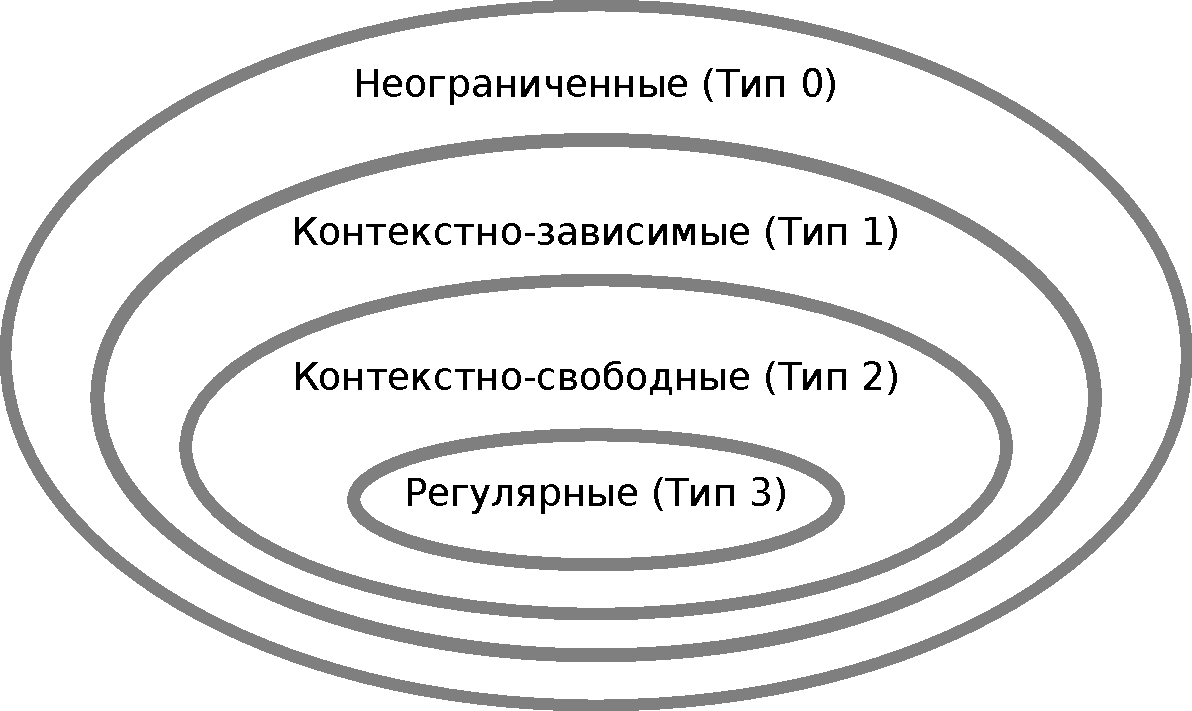
\includegraphics[width=0.9\textwidth]{figures/Chomsky.pdf}
    \end{center}
\end{figure}

Однако, данная иерархия постепенно теряет свою актуальность, так как появляются новые классы языков, свойства которых уже не удаётся адекватным образом отобразить, используя её.

Один из вариантов иерархии языков, более полно отображающий современное состояние дел, предложен Александром Охотиным%
\sidenote{
    Иерархия и некоторые отражаемые ей свойства подробно обсуждаются в презентации Александра Охотина \enquote{Underlying principles and recurring ideas of formal grammars} (\url{https://users.math-cs.spbu.ru/~okhotin/talks/grammars_lata_talk.pdf}).
    Также, с данной презентацией рекомендуется ознакомиться чтобы представить себе состояние области в целом.
}.
Вариация предложенной Александром Охотиным иерархии представлена на изображении~\ref{fig:hierarchyOkhotin}~
\sidenote{Данная вариация скомпонована из версии, представленной в презентации \enquote{Underlying principles and recurring ideas of formal grammars} и версии, взятой из работы~\cite{MRYKHIN2023113829}.}.
Приведённая диаграмма содержит регулярные и контекстно-свободные.
Так и подклассы, лежащие между ними.
Вместе с этим, классы, лежащие выше контекстно-свободных: многокомпонентные контекстно-свободные, булевы, конъюнктивные, их подклассы.

\begin{figure*}[h!]
    \caption{Иерархия. \emph{Reg}~--- регулярные, \emph{LLLin}, \emph{LRLin}, \emph{UnambLin}, \emph{Lin}, \emph{LL}, \emph{LR}, \emph{Unamb}~--- однозначные, \emph{Ordinary}~--- обыкновенные (контекстно-свободные)
        \emph{Conj}~--- конъюнктивные, \emph{Boolean}~--- булевы, \emph{UnamnbBool}, \emph{UnambConj}, \emph{VPDA}, \emph{LinConj}, \emph{UnambTAG}, \emph{TAG}, \emph{MCFL},}
    \label{fig:hierarchyOkhotin}
    \begin{center}
        \begin{tikzpicture}[node distance=1.0cm,bend angle=45,auto]
            \tikzstyle{lang}=[circle,thick,draw=blue!75,fill=blue!75,minimum size=1mm]
            \node [lang] (reg) [label=below:\emph{Reg}] {};
            \node [right of = reg] (reg_dummy) {};
            \node [lang] (lllin) [right of=reg_dummy, label=below:\emph{LLLin}] {};
            \node [right of = lllin] (lllin_dummy) {};
            \node [lang] (lrlin) [right of=lllin_dummy, label=below:\emph{LRLin}] {};
            \node [right of = lrlin] (lrlin_dummy) {};
            \node [lang] (unamblin) [right of=lrlin_dummy, label=below:\emph{UnambLin}] {};
            \node [right of = unamblin] (unamblin_dummy) {};
            \node [lang] (lin) [right of=unamblin_dummy, label=below:\emph{Lin}] {};
            \node [right of = lin] (lin_dummy) {};
            \node [right of = lin_dummy] (lin_dummy_2) {};
            \node [right of = lin_dummy_2] (lin_dummy_3) {};
            \node [lang] (conj) [right of=lin_dummy_3, label=below:\emph{Conj}] {};
            \node [right of = conj] (conj_dummy) {};
            \node [lang] (bool) [right of=conj_dummy, label=right:\emph{Bool}] {};

            \node [above of = lrlin] (lrlin_up_dummy) {};
            \node [lang] (ll) [above of=lrlin_up_dummy, label=above:\emph{LL}] {};
            \node [right of = ll] (ll_dummy) {};
            \node [lang] (lr) [right of=ll_dummy, label=above:\emph{LR}] {};
            \node [right of = lr] (lr_dummy) {};
            \node [lang] (unamb) [right of=lr_dummy, label=above:\emph{Unamb}] {};
            \node [right of = unamb] (unamb_dummy) {};
            \node [lang] (ordinary) [right of=unamb_dummy, label=right:\emph{Ordinary}] {};

            \node [lang] (conjleftcontext) [above of=conj_dummy, label=right:\emph{Conj$+\lhd$}] {};

            \node [below of = lrlin] (lrlin_down_dummy) {};
            \node [lang] (vpda) [below of=lrlin_down_dummy, label=below:\emph{VPDA}] {};
            \node [below of = lin] (lin_down_dummy_1) {};
            \node [below of = lin_down_dummy_1] (lin_down_dummy_2) {};
            \node [right of = lin_down_dummy_2] (lin_right_dummy_1) {};
            \node [lang] (linconj) [right of=lin_right_dummy_1, label=below:\emph{LinConj}] {};

            \node [lang] (unambtag) [above of=unamb_dummy, label=above:\emph{UnambTAG}] {};
            \node [right of = unambtag] (unambtag_dummy) {};
            \node [lang] (tag) [right of=unambtag_dummy, label=above:\emph{TAG}] {};
            \node [right of = tag] (tag_dummy) {};
            \node [lang] (mcfl) [right of=tag_dummy, label=above:\emph{MCFL}] {};

            \node [above of = linconj] (linconj_above_dummy) {};
            \node [lang] (unambconj) [right of=linconj_above_dummy, label=below:\emph{UnambConj}] {};
            \node [right of = unambconj] (unambconj_dummy) {};
            \node [lang] (unambbool) [right of=unambconj_dummy, label=right:\emph{UnambBool}] {};

            \node [below of = linconj] (linconj_below_dummy) {};
            \node [lang] (rtca) [right of=linconj_below_dummy, label=below:\emph{RT-CA}] {};
            \node [right of = rtca] (rtca_dummy) {};
            \node [lang] (ltca) [right of=rtca_dummy, label=right:\emph{LT-CA}] {};

            \path[->]
            (reg) edge node {} (lllin)
            (lllin) edge node {} (lrlin)
            (lrlin) edge node {} (unamblin)
            (unamblin) edge node {} (lin)

            (lllin) edge node {} (ll)
            (ll) edge node {} (lr)
            (ll) edge node {} (lr)
            (lr) edge node {} (unamb)
            (unamb) edge node {} (ordinary)

            (lrlin) edge node {} (lr)
            (unamblin) edge node {} (unamb)
            (lin) edge node {} (ordinary)

            (reg) edge node {} (vpda)
            (vpda) edge node {} (lr)
            (vpda) edge node {} (linconj)

            (ordinary) edge node {} (conj)
            (conj) edge node {} (bool)
            (conj) edge node {} (conjleftcontext)

            (unamb) edge node {} (unambtag)
            (ordinary) edge node {} (tag)
            (unambtag) edge node {} (tag)
            (tag) edge node {} (mcfl)

            (lin) edge node {} (linconj)
            (linconj) edge node {} (unambconj)
            (unambconj) edge node {} (unambbool)
            (unambconj) edge node {} (conj)
            (unambbool) edge node {} (bool)
            (unamb) edge node {} (unambconj)

            (linconj) edge node {} (rtca)
            (rtca) edge node {} (ltca)
            ;
        \end{tikzpicture}
    \end{center}
\end{figure*}

Для того, чтобы содержательно рассуждать про различные классы языков, необходимо иметь механизм, позволяющий чётко отделить один класс от другого.
\emph{Лемма о накачке} для соответствующего класса~--- один из классических таких механизмов.
Однако, не для всех классов языков соответствующие результаты получены.
Так, например, формулировка леммы о накачки для многокомпонентных контекстно-свободных языков в общем виде всё ещё не найдена, хотя существуют формулировки для отдельных подклассов.
Аналогично, для булевых и конъюнктивных языков всё ещё не предложены аналоги лемм о накачке.


%\section{Вопросы и задачи}
%\begin{enumerate}
%  \item !!!
%  \item !!!
%\end{enumerate}

\setchapterpreamble[u]{\margintoc}
\chapter{Регулярные языки}
\tikzsetfigurename{RegularLanguages_}

В данном разделе мы обсудим регулярные языки~--- класс, лежащий на самом нижнем уровне иерархии Хомского.
Будут рассмотрены основные способы задания таких языков: \emph{регулярные выражения}, \emph{конечные автоматы}, \emph{лево(право)линейные грамматики}.
Обсудим основные свойства регулярных языков, такие как замкнутость относительно различных операций, а также различные свойства соответствующих автоматов и грамматик.

\section{Регулярные выражения}

Регулярные выражения~--- один из классических способов задать регулярный язык%
\sidenote[][*6]{
    Замечание для программистов.
    Важно понимать, что речь идёт о формальной конструкции, а не о том, что называется регулярными выражениями в различных языках программирования или библиотеках, где под названием \enquote{регулярные выражения} могут скрываться конструкции, существенно более выразительные, чем обсуждаемые здесь.
}.
Основывается этот способ на предложении синтаксиса для описания \emph{регулярных множеств}%
\sidenote{Помним, что язык~--- это множество слов.}.

\begin{definition}[Регулярное множество]
    Регулярное множество (над алфавитом $\Sigma$) это:
    \begin{itemize}
        \item $\varnothing$;
        \item $\{\varepsilon\}$;
        \item $\{t\}$, $t \in \Sigma$;
        \item $R_1 \cup R_2$, где $R_1$ и $R_2$~--- регулярные множества;
        \item $R_1 \cdot R_2$, где $R_1$ и $R_2$~--- регулярные множества;
        \item $R^*$, где $R$~--- регулярное множество.
    \end{itemize}
\end{definition}

Для того, чтобы описывать такие множества, удобно пользоваться \emph{регулярными выражениями}.

\begin{definition}[Регулярное выражение]
    Регулярное выражение (над алфавитом $\Sigma$) это:
    \begin{itemize}
        \item $\varnothing$;
        \item $\varepsilon$;
        \item $t$, $t \in \Sigma$;
        \item $R_1 \mid R_2$, где $R_1$ и $R_2$~--- регулярные выражения;
        \item $R_1 \cdot R_2$, где $R_1$ и $R_2$~--- регулярные выражения;
        \item $R^*$, где $R$~--- регулярное выражение;
        \item $(R)$, где $R$~--- регулярное выражение.
    \end{itemize}
\end{definition}

Отметим несколько важных с прикладной точки зрения моментов.
Во-первых, часто используется расширенный синтаксис, в который добавляются конструкции не увеличивающие выразительную силу, но упрощающие запись.
Например, встречаются следующие расширения%
\sidenote{
    Существуют и другие, однако их мы не будем использовать и, соответственно, рассматривать.
    Читатель может вспомнить, что называется регулярными выражениями в его любимом языке программирования и попробовать самостоятельно выразить имеющиеся там конструкции через базовые.}.
\begin{itemize}
    \item $R? = R \mid \varepsilon$, где $R$~--- регулярное выражение.
    \item $R^+ = R \cdot R^*$, где $R$~--- регулярное выражение.
\end{itemize}

Во-вторых, конструкции $\varnothing$ и $\varepsilon$ используются крайне редко, особенно в случае расширенного синтаксиса, так как часто выражение, эквивалентное использующему данные конструкции, более компактно записывается с использованием расширенного синтаксиса.
В-третьих, оператор конкатенации часто опускается%
\sidenote{Как и знак умножения во многих математических записях.}.

Рассмотрим несколько примеров регулярных выражений.
\begin{example}
    Регулярное выражение $a$ задаёт регулярное множество $\{a\}$ и, соответственно, язык из единственного слова $a$.
\end{example}


\begin{example}
    Регулярное выражение $ab$ задаёт регулярное множество $\{ab\}$ и, соответственно, язык из единственного слова $ab$.
\end{example}


\begin{example}\label{exmpl:regexp_a_star}
    Регулярное выражение $a^*$ задаёт регулярное множество $$R = \bigcup_{i=0}^{\infty}{a^i} = \{\varepsilon, a, aa, aaa, \ldots \}$$ и, соответственно, бесконечный язык, содержащий для любого неотрицательного целого $n$ цепочку из символов $a$ длины $n$.
\end{example}

\begin{example}
    Регулярное выражение $a^*b$ задаёт бесконечный язык, содержащий цепочки, полученные конкатенацией цепочек из языка, описанного в примере~\ref{exmpl:regexp_a_star} и символа $b$.
    Иными словами, любая цепочка из языка выглядит как последовательность символов $a$ произвольной длины (возможно пустая), за которой следует символ $b$.
    Примеры цепочек из языка: $b, ab, aaab, aaaaab$.
\end{example}

\begin{example}
    Регулярное выражение $(a\mid b)^*$ задаёт бесконечный язык, цепочки которого имеют произвольную длину и состоят из символов $a$ и $b$ в произвольном порядке.
    Примеры цепочек из языка: $\varepsilon, a, aa, b, ba, aba$.
\end{example}

\begin{example}
    Регулярное выражение\sidenote{Здесь мы воспользовались расширенным синтаксисом.} $(ab)^*c?$ задаёт бесконечный язык, цепочки которого состоят их произвольного количества повторений подпоследовательности $ab$ за которой может следовать (но не обязательно следует) символ $c$.
    Примеры цепочек из языка: $\varepsilon, abab, abc, abababc$.
\end{example}

\section{Конечные автоматы}

\emph{Конечный автомат}~--- вычислительная машина, которая имеет конечный набор состояний и может совершать переходы между ними, основываясь на прочитанных входных данных.
Важно отметить, что ни какой дополнительной памяти классический конечный автомат не имеет%
\sidenote{Существуют, например, автоматы с константным объёмом дополнительной памяти (регистрами)~\cite{!!!}} и не производит дополнительных действий%
\sidenote{Cуществуют автоматы с записью на отдельную (выходную) ленту, и т.д.~\cite{!!!}}.

\begin{definition}[Недетерминированный конечный автомат]
    \label{def:NondeterminicticFiniteAutomata}
    \emph{Недетерминированный конечный автомат} (НКА)~--- это пятёрка $M = \langle Q, Q_S, Q_F, \delta, \Sigma \rangle$, где
    \begin{itemize}
        \item $Q$~--- конечное множество состояний, $Q \neq \varnothing$;
        \item $Q_S \subseteq Q$~--- множество стартовых состояний, $Q_S \neq \varnothing$;
        \item $Q_F \subseteq Q$~--- множество финальных состояний\sidenote{Обатите внимание, множества стартовых и финальных состояний могут перескаться.}, $Q_F \neq \varnothing$;
        \item $\delta \subseteq Q \times (\Sigma \cup \varepsilon) \times 2^Q$~--- функция переходов, а $\varepsilon \notin \Sigma$;
        \item $\Sigma$~--- конечный алфавит.
    \end{itemize}
\end{definition}

Заметим, что функцию переходов можно представить разными способами: это может быть множество троек вида $(q_i, t, q_j)$, матрица, или же граф с метками на рёбрах $G = \langle Q, \{(q_i,t,q_j \mid q_j \in \delta(q_i,t))\}, \Sigma \rangle$.
В дальнейшем мы чаще всего будем использовать представление автомата в виде графа.
Чтобы такое представление было полным, в графе отдельно обозначают стартовые и финальные состояния, как это показано на рисунках~\ref{fa:start_state} и~\ref{fa:final_state} соответственно.
\begin{marginfigure}    
    \begin{center}
        \begin{tikzpicture}
            \node[state,initial] (q_0)  {$q_s$};
        \end{tikzpicture}
    \end{center}
    \caption{Пример обозначения стартового состояния $q_s$}
    \label{fa:start_state}
\end{marginfigure}
\begin{marginfigure}    
    \begin{center}
        \begin{tikzpicture}
            \node[state,accepting] (q_0)  {$q_f$};
        \end{tikzpicture}
    \end{center}
    \caption{Пример обозначения финального состояния $q_f$}
    \label{fa:final_state}
\end{marginfigure}

Так как нас интересуют конечные автоматы в контексте языков, то будем говорить, что на ленте автомата записано какое-то слово (или строка).
Иными словами, будем говорить, что автомат принимает на вход слово или строку.
При таком подходе автомат естественно рассматривать как \emph{распознователь}\sidenote{Хотя на автомат можно смотреть и как на генератор: любой путь от сартового состояния до финального задаёт слово из языка.}.

\begin{example}
    Пусть задан автомат $M=\langle Q, Q_S, Q_F, \delta, \Sigma\rangle$, где
    \begin{itemize}
        \item $Q = \{0,1,2\}$;
        \item $Q_S = \{0\}$;
        \item $Q_F = \{1\}$;
        \item $\Sigma = \{a,b\}$;
        \item $\delta$ определена следующим образом\sidenote{Часто указывают только те случаи, в которых $\delta$ возвращет непустое множество. Тогда для неуказанных входных аргументов $\delta$ возвращает пустое множество.}: 
        \begin{alignat*}{6}
            \delta(0,a) =& \{0,1\}      \quad    & \delta(1,a) =& \varnothing \quad & \delta(2,a) =& \varnothing \\
            \delta(0,b) =& \varnothing           & \delta(1,b) =& \{2\}             & \delta(2,b) =& \{1\} \\
            \delta(0,\varepsilon) =& \varnothing & \delta(1,\varepsilon) =& \{0\}   & \delta(2,\varepsilon) =& \varnothing.
        \end{alignat*}
    \end{itemize}
    Тогда его можно представить в виде графа как показано на рисунке~\ref{fa:fa_example}.
    \begin{marginfigure}    
        \begin{center}
            \begin{tikzpicture}
                \node[state,initial] (q_0) {$0$};
                \node[state,accepting] (q_1) [right = of q_0] {$1$};
                \node[state] (q_2) [above = of q_1] {$2$};
                \path[->]
                    (q_0) edge[bend left, above]   node {$a$} (q_1)
                    (q_0) edge[loop above, above]   node {$a$} (q_0)
                    (q_1) edge[bend left, left]   node {$b$} (q_2)
                    (q_2) edge[bend left, right]   node {$b$} (q_1)
                    (q_1) edge[bend left, below]  node {$\varepsilon$} (q_0);
            \end{tikzpicture}
        \end{center}
        \caption{Пример конечного автомата}
        \label{fa:fa_example}
    \end{marginfigure}
\end{example}

Процесс вычислений, проделываемых конечным автоматом, удобно описывать в терминах переходов между \emph{конфигурациями}.

\begin{definition}[Конфигурация]
    Конфигурация $c$ конечного автомата $M = \langle Q, Q_S, Q_F, \delta, \Sigma \rangle$~--- это пара $(q, w)$, где $q\in Q$~--- это текущее состояние автомата, а $w \in \Sigma^*$~--- непросмотренная часть входной строки.
\end{definition}

\begin{definition}[Переход в НКА]
    Будем говорить, что автомат $M = \langle Q, Q_S, Q_F, \delta, \Sigma \rangle$ может перейти из конфигурации $c_1 = (q_1, w_1)$ в конфигурацию $c_2 = (q_2, w_2)$, если
    \[c_2 \in \{(q_2,w_2) \mid w_1 = aw_2, (q_1,a, q_2) \in \delta\} \cup \{(q_2,w_1) \mid (q_1, \varepsilon, q_2) \in \delta\}.\]
    Обозначать этот факт будем как $c_1 \to c_2$.
    Также будем считать, что на множестве конфигураций задано отношение перехода $(\to):(Q \times \Sigma^*)\times(Q \times \Sigma^*)$.
    
\end{definition}

\begin{definition}
    Транзитивное замыкание отношения перехода на конфигурациях будем обозначать следующим образом: $$ c_1 \to^* c_2. $$
    Альтернативно, в случае если $c_1 \to^* c_2$, будем говорить, что конфигурация $c_2$ \textit{достижима} из конфигурации $c_1$.
\end{definition}

Для удобства работы с недетерминированными автоматами расширим это отношение на множество конфигураций.

\begin{definition}
Будем говорить, что автомат может перейти из множества конфигураций $C_1$ в множество конфигураций $C_2$, если 
$$C_2 = \bigcup_{c_1 \in C_1} \{c_2 \mid c_1 \to c_2 \}.$$

Обозначать этот факт будем как  $C_1 \Rightarrow C_2 $.
\end{definition}

\begin{definition}
Транзитивное замыкание отношения перехода на множествах конфигураций будем обозначать следующим образом: $$ C_1 \Rightarrow^* C_2. $$
\end{definition}

Для описания работы автомата $M = \langle Q, Q_S, Q_F, \delta, \Sigma \rangle$ нам понадобятся следующие выделенные типы конфигураций.
\begin{itemize}
    \item Стартовая конфигурация $c_s = (q_s,w)$, $q_s \in Q_S$, $w$ --- цепочка, которая подаётся на вход автомату. 
    Для недетерминированного автомата естественно задать множество стартовых конфигурация $C_S = \bigcup_{q_s \in Q_S} (q_s,w)$.
    \item Финальная (принимающая) конфигурация $c_f = (q_f,\varepsilon)$, $q_f \in Q_F$.
\end{itemize}

Таким образом, работу автомата можно описать как последовательность переходов между множествами конфигураций. 
Работа начинается с множества стартовых конфигураций и завершается в следующих двух случаях.
\begin{enumerate}
    \item Очередное множество конфигураций содержит финальную конфигурацию:
    $$c_f \in C_S \text{ или } C_S \Rightarrow^* C_i, c_f \in C_i.$$ В этом случае говорят, что автомат \textit{принимает} входную строку.
    \item Очередное множество конфигураций пусто:
    $$C_0 = C_S \Rightarrow^* C_i \Rightarrow^* \varnothing, \text{ для любого } i: c_f \notin C_i.$$ 
    В этом случае говорят, что автомат \textit{не принимает} или \textit{отвергает} входную строку.
\end{enumerate} 

\begin{definition}
    Язык задаваемый автоматом $$\{w \mid \}$$
\end{definition}

Так как конфигурация полностью описывает состояние процесса вычислений, то не надо обрабатывать одну и ту же конфигурацию несколько раз. 
Это поможет при написании реального интерпретатора. 
Будем отслеживать уже посещённые (обработанные) конфигурации\sidenote{Техника, аналогичная той, что применяется в обходах графов (обход в ширину, обход в глубину) для того, чтобы избежать повторного посещения вершин и, как следствие, зацикливания обхода. Более того, она типична для алгоритмов с рабочим множеством.}. 

\begin{example}
    Пример интерпретации конечного автомата.
\end{example}

\begin{definition}[Детерминированный конечный автомат]
    \label{def:DeterminicticFiniteAutomata}
    \emph{Детерминированный конечный автомат} (ДКА, Deterministic Finite Automata, DFA)~--- это пятёрка $M = \langle Q, q_S, Q_F, \delta, \Sigma \rangle$, где
    \begin{itemize}
        \item $Q$~--- конечное множество состояний, $Q \neq \varnothing$;
        \item $q_S \in Q$~--- стартовое состояние;
        \item $Q_F \subseteq Q$~--- множество финальных состояний\sidenote{Обатите внимание, стартовое состояниеможет входить в множество финальных.}, $Q_F \neq \varnothing$;
        \item $\delta \subseteq Q \times \Sigma \times Q$~--- функция переходов\sidenote{При данном определении автомат будет ещё и \emph{полным}: для каждого состояния и каждого символа определён переход. Часто встречается вариант, когда функция переходов частично определёна: для некоторых состояний не определены переходы для некоторых символов.};
        \item $\Sigma$~--- конечный алфавит.
    \end{itemize}
\end{definition}

Основных отличий от недетерминированного автомата два.
Во-первых, стартовое состояние ровно одно.
Во-вторых,  функция переходов не допускает переходов по $\varepsilon$ и из любого состояния существует не более одного перехода по конкретному символу.

\begin{example}
    Пример КА.
    % \begin{tikzpicture}

    % \end{tikzpicture}
\end{example}

\begin{example}
    Пример интерпретации конечного автомата.
\end{example}

\section{Производные для регулярных языков}

Предложены в~\sidecite{Brzozowski1964}

По мотивам~\sidecite{OWENS_REPPY_TURON_2009}

\begin{itemize}
    \item $\partial_t(\varepsilon) = \varnothing$
    \item $\partial_t(\varnothing) = \varnothing$
    \item $\partial_t(x) = $
    \item $\partial_t(R_1 \cdot R_2) = \partial_t(R_1) \cdot (R_2) \mid $
    \item $\partial_t(R_1 \mid R_2) = \partial_t(R_1) \mid \partial_t(R_2) $
    \item $\partial_t(R^*) = $\sidenote{Интересное упражнение --- показать это, расписав по определению звезду Клини.}
\end{itemize}

Проверка на пустоту (часто isNull).

\begin{itemize}
    \item $IsNull(\varepsilon) = false$
    \item $\partial_t(\varnothing) = \varnothing$
    \item $\partial_t(x) = $
    \item $\partial_t(R_1 \cdot R_2) = \partial_t(R_1) \cdot (R_2) \mid $
    \item $\partial_t(R_1 \mid R_2) = \partial_t(R_1) \mid \partial_t(R_2) $
    \item $\partial_t(R^*) = $\sidenote{Интересное упражнение --- показать это, расписав по определению звезду Клини.}
\end{itemize}

Проверка пустоты регулярного языка\sidenote{Отдельное решение не на производных.}


\section{Построение конечного автомата по регулярному выражению}
 
На производных%
\sidenote{Существуют и другие алгоритмы построения автомата по регулярному выражению. Например, алгоритм Томпсона~\cite{10.1145/363347.363387} или алгоритм Глушкова~\cite{Glushkov1961}.
Как правило, каждый алгоритм строит автомат со специфичными свойствами: детерминированный или нет, с $\varepsilon$-переходами или без них.}.

Каждое состояние соответствует языку, распозноваемому из этого состояния.

Стартовое --- исходное регулярное выражение. Далее в цикле. 
Берём очередное необработанное состояние, по каждому символу из алфавита берём производную соответствующего ему регулярного выражения.
Добавляем получившееся состояние (если ещё не было такого).
Если состояние isNullable, то помечаем его финальным.
Добавляем ребро.

В результате получим полный детерминированный конечный автомат\sidenote{Формально можно получить минимальный, но на практике это сложно. Но часто всё же достаточно близко к минимальному получается.}.  

Примеры.


\section{Построение регулярного выражения по конечному автомату}

Алгоритм Клини(?)
Регулярное выражение будем строить по недетерминированному автомату специального вида: потребуем, чтобы у него было ровно одно стартовое состояние и ровно одно финальное%
\sidenote{Любой автомат можно привести к такому виду. 
Предположим, что в автомате два стартовых состояния $q_0^s$ и $q_1^s$.
Добавим новое сотояние $q_s$, назначим его стартовым, добавим переходы $q_s \xrightarrow{\varepsilon} q_0^s$ и $q_s \xrightarrow{\varepsilon} q_1^s$, уберём $q_0^s$ и $q_1^s$ из стартовых.
Аналогично можно поступить и с финальными состояниями.}. 
\begin{marginfigure}    
    \begin{center}
        \begin{tikzpicture}

            \node[state] (q_0)                   {$q_i$};
            \node[state] (q_1) [right = 1.8 of q_0]  {$q_j$};

            \path[->]
                (q_0) edge[bend left = 45, above]   node {$R_1$} (q_1)
                (q_0) edge[above]   node {$R_2$} (q_1)
                (q_0) edge[bend right, below]  node {$R_3$} (q_1);

        \end{tikzpicture}
    \end{center}
    \caption{Два состояния с параллельными рёбрами}
    \label{fa:fa1}
\end{marginfigure}
\begin{marginfigure}
    
    \begin{center}
        \begin{tikzpicture}

            \node[state] (q_0)                    {$q_i$};
            \node[state] (q_1) [right = 1.8 of q_0]  {$q_j$};
            
            \path[->]
                (q_0) edge[above]  node {$R_1 \mid R_2 \mid R_3$} (q_1);

        \end{tikzpicture}
    \end{center}
    \caption{Результат объединения параллельных рёбер для состояний, представленных на рисунке~\ref{fa:fa1}}
    \label{fa:fa2}
\end{marginfigure}

Будем в цикле выполнять последовательно две операции.
\begin{enumerate}
    \item Объединение параллельных рёбер.
    \item Устранение состояния $v$. За один шаг можем устранить любое состояние кроме стартового или финального.
\end{enumerate}
Цикл повторяется до тех пор, пока в автомате не останется ровно два состояния: стартовое и финальное.
После завершения цикла необходимо ещё раз объединить параллельные рёбра. 
После этого, по полученному автомату можно построить итоговое регулярное выражение.

Параллельные рёбра вида $p_i \xrightarrow{R_1} q_i, \ldots, p_i \xrightarrow{R_k} q_i$ объединяются в одно ребро вида $p_i \xrightarrow{R_1 \mid \ldots \mid R_k} q_i$, метка которого --- объединение всех регулярных выражений с параллельных рёбер.
Пример такого объединения приведён на рисунках~\ref{fa:fa1} и~\ref{fa:fa2}.

Операция устранения состояния $v$ устроена следующим образом. 
Рассмотрим три типа рёбер.
\begin{enumerate}
    \item Рёбра вида $p_i \xrightarrow{R_{p_i}} v$, где $p_i \neq v$.
    \item Рёбра вида $v \xrightarrow{R_{q_j}} q_i$, где $q_i \neq v$.
    \item Рёбра вида\sidenote{Рёбер такого вида для заданной вершины всегда не более одного, так как мы производим объеднинение параллельных рёбер на каждой итерации алгоритма.} $v \xrightarrow{R_v} v$.
\end{enumerate}

В результате устранения состояния $v$ все рассмотренные рёбра должны быть удалены. 
Взамен них должны быть добавлены рёбра вида $p_i \xrightarrow{R_{p_i} \cdot R_v^* \cdot R_{q_j}} q_j$.
Пример описанного преобразования представлен на рисунках~\ref{fa:fa3} и~\ref{fa:fa4} 

\begin{figure}
    \begin{center}
        \begin{subfigure}[b]{0.47\textwidth}
            \begin{center}
                
                \begin{tikzpicture}

                \node[state] (p_0)          {$p_0$};
                \node[text width=0.3cm]  (p_1) [below = 0.3 of p_0] {$\vdots$}; 
                \node[state] (p_2) [below = 0.3 of p_1]  {$p_i$};
                \node[text width=0.3cm] (p_3) [below = 0.3 of p_2]  {$\vdots$};
                \node[state] (v_0) [right = of  p_2] {$v$};
                \node[state] (q_2) [right = of v_0] {$q_j$};
                \node[text width=0.3cm] (q_1) [above = 0.3 of  q_2]  {$\vdots$};
                \node[state] (q_0) [above = 0.3 of q_1]  {$q_0$};
                \node[text width=0.3cm] (q_3) [below = 0.3 of q_2]  {$\vdots$};

                \path[->]
                    (p_0) edge[above]  node {$R_{p_0}$} (v_0)
                    (p_2) edge[below]  node {$R_{p_i}$} (v_0)
                    (v_0) edge[left]  node {$R_{q_0}$} (q_0)
                    (v_0) edge[below]  node {$R_{q_j}$} (q_2)
                    (v_0) edge[loop above, above]  node {$R_v$} (v_0);

                \end{tikzpicture}
            \end{center}
        
            \caption{Автомат перед устранением состояния $v$}
            \label{fa:fa3}

        \end{subfigure}\hspace{5mm}
        \begin{subfigure}[b]{0.47\textwidth}
            \begin{center}

                \begin{tikzpicture}

                    \node[state] (p_0)          {$p_0$};
                    \node[text width=0.3cm]  (p_1) [below = 0.3 of p_0] {$\vdots$}; 
                    \node[state] (p_2) [below = 0.3 of p_1]  {$p_i$};
                    \node[text width=0.3cm] (p_3) [below = 0.3 of p_2]  {$\vdots$};
                    
                    \node[text width=0.3cm] (v_0) [right = of p_2] {};

                    \node[state] (q_2) [right = of v_0] {$q_j$};
                    \node[text width=0.3cm] (q_1) [above = 0.3 of q_2]  {$\vdots$};
                    \node[state] (q_0) [above = 0.3 of q_1]  {$q_0$};
                    \node[text width=0.3cm] (q_3) [below = 0.3 of q_2]  {$\vdots$};        
                    
                    \path[->]
                    (p_0) edge[bend left, above]  node {$R_{p_0} R_v^* R_{q_0}$} (q_0)
                    (p_0) edge[bend left, left]  node {$R_{p_0} R_v^* R_{q_j}$} (q_2)
                    (p_2) edge[bend right, left]  node {$R_{p_i} R_v^* R_{q_0}$} (q_0)
                    (p_2) edge[bend right, below]  node {$R_{p_0} R_v^* R_{q_0}$} (q_2);

                \end{tikzpicture}
            
            \end{center}
            
            \caption{Результат устранения состояния $v$ для автомата, представленного на рисунке~\ref{fa:fa3}}
            \label{fa:fa4}
        \end{subfigure}
    \end{center}
    \caption{Общая схема устранения состояния $v$ при построении регулярного выражения по конечному автомату}
    \label{fa:fa_3_4}    
\end{figure}

После завершения основного цикла (когда в автомате осталось ровно два состояния), необходимо ещё раз объединить параллельные рёбра.
Общий вид получившегося автомата представлен на рисунке~\ref{fa:fa5}.
По такому автомату строим выражение вида \[(R_1^* \cdot (R_2 \cdot R_3^* \cdot R_4 )^* \cdot R_2 \cdot R_3^*,\] которое и будет ответом.
\begin{marginfigure}
    
    \begin{center}
        \begin{tikzpicture}

            \node[state, initial] (q_0)          {$0$};
            \node[state, accepting] (q_1) [right = of q_0]  {$1$};
            \path[->]
                (q_0) edge[bend left, above]  node {$R_2$} (q_1)
                (q_1) edge[bend left, below]  node {$R_4$} (q_0)
                (q_1) edge[loop above, above]  node {$R_3$} (q_1)
                (q_0) edge[loop above, above]  node {$R_1$} (q_0);

        \end{tikzpicture}

    \end{center}

    \caption{Общий вид автомата после завершения основного цикла}
    \label{fa:fa5}

\end{marginfigure}

\begin{example}
    Примеры.
\end{example}


\section{Лево(право)линейные грамматики}

Наложив некоторые ограничения на внешний вид правил грамматики можно получить грамматики, задающие регулярные языки.

\begin{definition}[Леволинейная грамматика]
    Грамматика $G=\langle \Sigma, N, P, S \rangle$ называется леволиненйной, если все её правила имеют вид
    \[N_i \to \alpha w,\]
    где $N_i \in N$, $\alpha \in \{\varepsilon\} \cup N$, $w \in \Sigma ^*$.
\end{definition}

\begin{definition}[Праволинейная грамматика]
    Грамматика $G=\langle \Sigma, N, P, S \rangle$ называется праволиненйной, если все её правила имеют вид
    \[N_i \to  w \alpha,\]
    где $N_i \in N$, $\alpha \in \{\varepsilon\} \cup N$, $w \in \Sigma ^*$.
\end{definition}

Ноам Хомский и Джордж Миллер в работе~\sidecite{chomsky1958finite} показали, что лево(право)линейные грамматики задают регулярные языки.
Приведём процедуры построения автомата по грамматике и наоборот, грамматики по автомату.

Пусть дан конечный автомат $M = \langle \Sigma, Q, q_s, Q_f, \delta \rangle$. По нему можно построить праволинейную грамматику $G=\langle \Sigma, N, S, P \rangle$, где
\begin{itemize}
    \item $N = Q$
    \item $P = \{ q_i \to t q_j \mid (q_i, t, q_j)\in \delta\} \cup \{ q_i \to \varepsilon \mid q_i \in Q_F\}$
    \item $S = q_s$
\end{itemize}

Аналогичным образом строится автомат по праволинейной грамматике.
Упростить процедуру можно если заранее привести правила к виду $N_i \to tN_j$, где $t\in \Sigma$, добавив необходимое количество новых нетерминалов:
правило вида $N_i \to twN_k$ преобразуется в два правила
\begin{align*}
    N_i & \to tN_l  \\
    N_l & \to wN_k,
\end{align*}
после чего аналогично преобразуется правило для $N_l$.

\begin{example}
Пример построения грамматики по автомату.
\end{example}

\begin{example}
Автомат по грамматике.
\end{example}

\section{Лемма о накачке}

Лемма о накачке для регулярных языков позволяет проверить, что заданный язык не является регулярным.

\begin{lemma}
    Пусть $L$~--- регулярный язык над алфавитом $\Sigma$, тогда существует такое $n$, что для любого слова $\omega \in L$, $|\omega| \geq n$ найдутся слова $x,y,z\in \Sigma^*$, для которых верно: $xyz = \omega, y\neq \varepsilon,|xy|\leq n$ и для любого $k \geq 0$  $xy^kz \in L$.
\end{lemma}

\begin{proofSketch}
    \begin{enumerate}
        \item Так как язык регулярный, то для него можно построить конечный автомат $M = \langle Q, q_s,Q_f, \delta, \Sigma \rangle$.
              В том числе, минимальный по количеству состояний.
        \item В качестве $n$ возьмём $|Q| + 1$.
        \item Легко заметить, что для любой цепочки $w \in L, |w| > n$ путь в автомате, соответствующий принятию данной цепочки, будет содержать хотя бы один цикл.
              Действительно, в ориентированном графе с $k$ вершинами (а именно таким является автомат по построению) максимальная длина пути без повторных посещений вершин (соответственно, без циклов) не больше $k - 1$.
        \item Выберем любой цикл. Он будет задавать искомые цепочки $x, y$ и $z$ так, как представлено на рисунке~\ref{fig:reg_lang_pumping_lemma}.
              Заметим, что вход в цикл и выход из него в общем случае могут не совпадать, что даёт несколько вариантов разбиения пути на части, и на рисунке представлен лишь один из возможных.
              \qedhere
    \end{enumerate}
\end{proofSketch}

\begin{figure}
    \caption{Иллюстрация идеи доказательства леммы о накачке для регулярных языков: любой путь в графе, длина которого достаточно большая, может быть разбит на три части из леммы ($x$~--- красный подпуть, $y$~--- синий, $z$~--- зелёный), а многократный проход по циклу $y$ позволяет \enquote{накачать} слово.}
    \label{fig:reg_lang_pumping_lemma}
    \begin{center}
        \begin{tikzpicture}[->]
            \node[state, initial] (q1) {$q_1$};
            \node[state, right = 2 of q1] (q2) {$q_2$};
            \node[state, accepting, right = 2 of q2] (q3) {$q_3$};
            \node[state, above = 2 of q2] (q4) {$q_4$};
            \draw (q1) edge[above, snake it] node{} (q2)
            (q2) edge[bend right, snake it, side by side={red}{blue}] node{} (q4)
            (q4) edge[bend right, snake it, color=blue] node[left]{$y$} (q2)
            (q4) edge[above, snake it, color=green] node[right]{$z$} (q3)
            (q1) edge[above, snake it, color=red] node{$x$} (q2)
            ;
        \end{tikzpicture}
    \end{center}

\end{figure}


\section{Замкнутость регулярных языков относительно теоретико-множественных операций}

\begin{theorem}
    Регулярные языки замкнуты относительно перечисленных ниже операций.
    \begin{enumerate}
        \item Пересечение
        \item Дополнение
        \item Обращение
        \item Разность
    \end{enumerate}
\end{theorem}

Линейная алгебра для работы с регулярными языками: пересечение, замыкание.

Построение пересечения через тензорное произведение автоматов.

Идея доказательства, что мы построили именно пересечение.

Пересечение через синхронный обход в ширину.

%\section{Вопросы и задачи}
%
%Построить базу.
%
%Научиться выполнять запросы через линейку.

\setchapterpreamble[u]{\margintoc}
\chapter{Контекстно-свободные языки и грамматики}
\label{CFG}
\tikzsetfigurename{CFG_}

Контекстно-свободные языки, являясь строгим расширением регулярных, находят своё применение в различных задачах анализа программного кода, биоинформатики~\sidecite{!!!}, и других задачах анализа данных.

\section{Основные определения}

\begin{definition}[Контекстно-свободная грамматика]
    \emph{Контекстно-свободная грамматика}~--- это четвёрка вида $\langle \Sigma, N, P, S \rangle$, где
    \begin{itemize}
        \item $\Sigma$~--- это терминальный алфавит;
        \item $N$~--- это нетерминальный алфавит;
        \item $P$~--- это множество правил (продукций), таких что каждая продукция имеет вид $N_i \to \alpha$, где $N_i \in N$ и $\alpha \in \{\Sigma \cup N\}^* \cup {\varepsilon}$;
        \item $S$~--- стартовый нетерминал.
              Отметим, что $\Sigma \cap N = \varnothing$.
    \end{itemize}
\end{definition}

\begin{example}
    \label{ex:binary_cfg}
    Грамматика, задающая язык целых чисел в двоичной записи без лидирующих нулей: $G = \langle \{0, 1, -\}, \{S, N, A\}, P, S \rangle$, где $P$ определено следующим образом:
    \begin{align*}
        S & \rightarrow 0 \mid N \mid - N              \\
        N & \rightarrow 1 A                            \\
        A & \rightarrow 0 A \mid 1 A  \mid \varepsilon
    \end{align*}
\end{example}

При спецификации грамматики часто опускают множество терминалов и нетерминалов, оставляя только множество правил.
При этом нетерминалы часто обозначаются прописными латинскими буквами, терминалы~--- строчными, а стартовый нетерминал обозначается буквой $S$.
Мы будем следовать этим обозначениям, если не указано иное.

\begin{definition}[Отношение непосредственной выводимости]
    \label{def derivability in CFG}
    \emph{Отношение непосредственной выводимости}. Мы говорим, что последовательность терминалов и нетерминалов $\gamma \beta \delta$ \emph{непосредственно выводится из} $\gamma \alpha \delta$ \emph{при помощи правила} $\alpha \rightarrow \beta$ ($\gamma \alpha \delta \derives[] \gamma \beta \delta$), если
    \begin{itemize}
        \item $\alpha \rightarrow \beta \in P$,
        \item $\gamma, \delta \in \{\Sigma \cup N\}^* \cup {\varepsilon}$.
    \end{itemize}
\end{definition}

\begin{definition}[Рефлексивно-транзитивное замыкание отношения]
    \emph{Рефлексивно-транзитивное замыкание отношения}~--- это наименьшее рефлексивное и транзитивное отношение, содержащее исходное.
\end{definition}

\begin{definition}[Отношение выводимости]
    \emph{Отношение выводимости} является рефлексивно-транзитивным замыканием отношения непосредственной выводимости; обозначается $\derives$.
    \begin{itemize}
        \item $\alpha \derives \beta$ означает $\exists \gamma_0, \dots, \gamma_k \in \{\Sigma \cup N\}^* \cup {\varepsilon}$:
              \[ \alpha \derives[] \gamma_0 \derives[] \gamma_1 \derives[] \dots \derives[] \gamma_{k-1} \derives[] \gamma_{k} \derives[] \beta;\]
        \item Транзитивность: $\forall \alpha, \beta, \gamma \in \{\Sigma \cup N\}^* \cup {\varepsilon}$: $\alpha \derives \beta$, $\beta \derives \gamma \derives[] \alpha \derives \gamma$;
        \item Рефлексивность: $\forall \alpha \in \{\Sigma \cup N\}^* \cup {\varepsilon}$: $\alpha \derives \alpha$;
        \item $\alpha \derives \beta$~--- $\alpha$ выводится из $\beta$;
        \item $\alpha \derives[k] \beta$~--- $\alpha$ выводится из $\beta$ за $k$ шагов;
        \item $\alpha \derives[+] \beta$~--- при выводе использовалось хотя бы одно правило грамматики.
    \end{itemize}
\end{definition}

\begin{example}
    Пример вывода цепочки $-1101$ в грамматике из примера~\ref{ex:binary_cfg}:
    \[
        S \derives[] - N \derives[] - 1 A \derives[] - 1 1 A \derives - 1 1 0 1 A \derives[] - 1 1 0 1
    \]
\end{example}

\begin{definition}[Вывод слова в грамматике]
    Слово $\omega \in \Sigma^*$ \emph{выводимо в грамматике} $\langle \Sigma, N, P, S \rangle$, если существует некоторый вывод этого слова из начального нетерминала $S \derives \omega$.

\end{definition}

\begin{definition}[Левосторонний вывод]
    \emph{Левосторонний вывод}. На каждом шаге вывода заменяется самый левый нетерминал.
\end{definition}

\begin{definition}[Правосторонний вывод]
    \emph{Правосторонний вывод}. На каждом шаге вывода заменяется самый правый нетерминал.
\end{definition}

\begin{example}
    Приведем пример левостороннего вывода цепочки $cbaa$ в грамматике:
    \begin{align*}
        S & \rightarrow A A \mid s          \\
        A & \rightarrow A A \mid B b \mid a \\
        B & \rightarrow c \mid d
    \end{align*}
    Жирным выделен нетерминал, заменяемый на каждом шагу вывода.
    \[ \mathbf{S} \derives[] \mathbf{A} A \derives[] \mathbf{B} b A \derives[] c b \mathbf{A} \derives[] c b \mathbf{A} A \derives[] c b a \mathbf{A} \derives[] c b a a \]
\end{example}

Аналогично левостороннему можно определить правосторонний вывод.

\begin{definition}[Язык]
    \emph{Язык, задаваемый грамматикой}~--- множество строк, выводимых в грамматике $L(G) = \{ \omega \in \Sigma^* \mid S \derives \omega \}$.
\end{definition}

\begin{definition}[Эквивалентные грамматики]
    Грамматики $G_1$ и $G_2$ называются \emph{эквивалентными}, если они задают один и тот же язык: $L(G_1) = L(G_2)$
\end{definition}

\begin{example}  Пример эквивалентных грамматик для языка целых чисел в двоичной системе счисления.

    \begin{tabular}{p{0.4\textwidth} | p{0.5\textwidth}}
        \[
            \begin{aligned}
                \Sigma & = \{ 0, 1, - \}                            \\
                N      & = \{ S, N, A \}                            \\~\\
                S      & \rightarrow 0 \mid N \mid - N              \\
                N      & \rightarrow 1 A                            \\
                A      & \rightarrow 0 A \mid 1 A  \mid \varepsilon \\
            \end{aligned}
        \]
         &
        \[
            \begin{aligned}
                \Sigma & = \{ 0, 1, - \}                            \\
                N      & = \{ S, A \}                               \\~\\
                S      & \rightarrow 0 \mid 1 A  \mid - 1 A         \\
                A      & \rightarrow 0 A \mid 1 A  \mid \varepsilon \\
            \end{aligned}
        \]
    \end{tabular}

\end{example}


\begin{definition}[Неоднозначная грамматика]
    \emph{Неоднозначная грамматика}~--- грамматика, в которой существует 2 и более левосторонних (правосторонних) выводов для одного слова.
\end{definition}

\begin{example}
    Неоднозначная грамматика для правильных скобочных последовательностей:
    \[
        S \to (S) \mid S S \mid \varepsilon
    \]
    Два различных левосторонних вывода строки $()()()$:
    \begin{gather*}
        S \derives[] S S \derives [] (S) S \derives[] () S \derives[] () S S \derives[] () (S) S \derives[] () () S \derives[] () () (S) \derives[] () () ()\\
        S \derives[] S S \derives[] S S S \derives[] (S) S S \derives[] () S S \derives[] () (S) S \derives[] () () S \derives[] () () (S) \derives[] () () ()
    \end{gather*}
\end{example}

\begin{definition}[Однозначная грамматика]
    \emph{Однозначная грамматика}~--- грамматика, в которой существует не более одного левостороннего (правостороннего) вывода для каждого слова.
\end{definition}

\begin{example}
    Однозначная грамматика для правильных скобочных последовательностей
    \[
        S \to (S)S \mid \varepsilon
    \]
\end{example}

\begin{definition}[Существенно неоднозначный язык]
    \emph{Существенно неоднозначные языки}~--- языки, для которых невозможно построить однозначную грамматику.
\end{definition}

\begin{example}
    Пример существенно неоднозначного языка
    \[\{a^n b^n c^m \mid n, m \in \BbbZ\} \cup \{a^n b^m c^m \mid n,m \in \BbbZ\}\]
\end{example}

\section{Рекурсивные автоматы и сети}

Рекурсивный автомат (Recursive state machine, RSM)~\sidecite{10.1145/1075382.1075387} или сеть~--- это представление контекстно-свободных грамматик, обобщающее конечные автоматы.
В нашей работе мы будем придерживаться термина \emph{рекурсивный автомат}.
Классическое определение рекурсивного автомата выглядит следующим образом.

\begin{definition}
    \emph{Рекурсивный автомат}~--- это кортеж $\mathcal{R} = \langle \mathcal{N},\Sigma,B,B_S,Q,Q_S\rangle$ where
    \begin{itemize}
       \item $N$~--- множество нетерминальных символов, 
       \item $\Sigma$~--- множество терминальных символов, 
       \item $Q$~--- множество состояний рекурсивного автомата, 
       \item $Q_S$~--- множество стартовых состояний всех \emph{блоков}, 
       \item $B=\{B_{N_i} \mid N_i \in \mathcal{N}\}$~--- множество блоков, где каждый \\ $B_{N_i} = \langle Q_{N_i}, q_S, Q_F^{N_i}, \delta \rangle$~--- это детерминированный конечный автомат, называемый \emph{блоком}.
             Здесь:  
            \begin{itemize}
                \item $Q_{N_i} \subseteq Q$~--- множество состояний блока, 
                \item $q_S \in Q_{N_i} \cap Q_S$~--- стартовое состояние блока, 
                \item $Q_F^{N_i} \subseteq Q_{N_i}$~--- множество финальных состояний блока, 
                \item $\delta \subseteq Q_{N_i} \times  (\Sigma\cup Q_S) \times Q_{N_i}$~--- функция переходов блока.
            \end{itemize}
       \item $B_S \in B$~--- стартовый блок рекурсивного автомата.
    \end{itemize}
\end{definition}

Таким образом, рекурсивный автомат~--- это набор детерминированных конечных автоматов над алфавитом $\Sigma \cup Q_S$.
В некоторых случаях наб будет удобно рассматривать этот набор как одн конечный автомат.
Однако процесс работы рекурсивного автомата несколько отличается от работы конечного автомата, хотя и похож на него.
Основное отличие~--- необходимость использовать стек для обработки переходов, помеченных элементами из $Q_S$.

По аналогии с конечными автоматами, процесс работы рекурсивных автоматов достаточно естественно описывается в терминах переходов между \emph{конфигурациями}.

\begin{definition}
    \emph{Конфигурация} $C_{\mathcal{R}}$ рекурсивного автомата $\mathcal{R}=\langle \mathcal{N},\Sigma,B,B_S,Q,Q_S \rangle$ over the graph $D=\langle V,E,L \rangle$ is a tuple $(q,v,\mathcal{S})$ where 
    \begin{itemize}
        \item $q \in Q$ is a current state of RSM,
        \item $\mathcal{S}$ is the current stack, whose frames have one of two types: 
        \begin{itemize} 
            \item return addresses frame (elements of $Q$) to specify states to continue computation after the call is finished;
            \item parsing tree node to store fragments of a parsing tree,
        \end{itemize}
        \item $v \in V$ is the current vertex (current position in the input).
    \end{itemize}
\end{definition}

\begin{definition}\label{def:rsm_transition}
    A \emph{transition step} of the RSM specifies how to get new configurations of RSM, given the current configuration. $C_{\mathcal{R}} \vdash W$ denotes that $\mathcal{R}$ can go to each configuration in $W$ from the configuration $C_{\mathcal{R}}$.
    \begin{align*}
    (q,v,w_0::s::\mathcal{S})  \vdash & \{ (q',v',t::w_0::s::\mathcal{S}) \mid (q,t,q') \in \delta, (v,t,v') \in E\} \\
                       & \cup \{(s', v, q'::w_0::s::\mathcal{S}) \mid (q,s',q') \in \delta, s' \in Q_S \} \\
                       & \cup \{(s,v,\emph{Node}(N_i, w_0)::\mathcal{S}) \mid q \in Q_F^{N_i}\}
    \end{align*}
    where $w_0$ is a possibly empty sequence of terminals and nonterminal nodes. 
\end{definition}

To simplify the acceptance condition, we introduce the concept of an \textit{extended RSM}. 

\begin{definition}
    For the given RSM $\mathcal{R}=\langle \mathcal{N},\Sigma,B,B_S,Q,Q_S\rangle$,
    the \textit{extended RSM} 
    $$\mathcal{R}'=\langle \mathcal{N} \cup \{S'\},\Sigma \cup\{\$\},B \cup {B'_S},B'_S,Q \cup \{q_0',q_1',q_2'\},Q_S \cup \{q_0'\}\rangle$$
    is an RSM which defines the same language and is built from $\mathcal{R}$ by adding a new start box 
    $$B'_S = \langle \{q_0',q_1',q_2'\}, q_0', \{q_2'\}, \{(q_0',q_0,q_1'),(q_1',\$, q_2')\} \rangle$$ where 
    \begin{itemize}
        \item $q_0$ is a start state of $B_S$,
        \item \$ is a special symbol to mark the end of input, $\$ \notin \Sigma$,
        \item $q_i'$ are newly added states, $q_i'\notin Q$.
    \end{itemize}
\end{definition} 

Finally, for the given extended RSM $\mathcal{R}$ and the given graph $D$ we say that $v_n$ is reachable from $v_0$  w.r.t. $\mathcal{R}$ if $(q'_0,v_0,[]) \vdash^* C$ such that $(q'_1,v_n,[N_S]) \in C$, where $\vdash^*$ denotes zero or more transition steps, and $N_S$ is a node for the start nonterminal of the original (not extended) RSM. Additionally, $N_S$ represents a respective path.

Now we need a way to compute transitions and to build trees efficiently, avoiding recomputation and infinite cycles that are possible with the naive implementation.
Moreover, we need a compact representation of all paths of interest whose number can be infinite.

\subsection{Example}\label{section:example_of_rsm}

\begin{marginfigure}
    \begin{center}
        \resizebox{\marginparwidth}{!}{
            \begin{tikzpicture}[->,>=stealth']  

                \node[initial,state]   (F)              {$q_4$};
                \node[state]           (G) [right = of F] {$q_5$};
                \node[accepting,state] (H) [right = of G] {$q_6$};
                \node[draw=black, fit= (F) (G) (H), inner sep=0.25cm] (J) {};
                \node[below right] at (J.north west) {S'};

                \path (F) edge[below]              node {$q_0$} (G)
                    (G) edge[below]              node {$\$$} (H); 

                \node[initial,state] (A) [below = 2.6cm of F] {$q_0$};
                \node[state]         (B) [right = of A] {$q_1$};
                \node[state]         (D) [above right = of B] {$q_2$};
                \node[accepting,state]         (C) [right = of B] {$q_3$};
                \node [draw=black, fit= (A) (C) (D), inner sep=0.25cm] (E) {};
                \node[below right] at (E.north west) {S};

                \path (A) edge[below]              node {a} (B)
                      (B) edge[left]               node {$q_0$} (D)
                          edge[below]              node {b} (C)
                      (D) edge[right]              node {b} (C);
            \end{tikzpicture}
       }
    \end{center}    
    \caption{Расширенный рекурсивный автомат для грамматики $S \to a \ b \mid a \ S \ b$}
    \label{fig:example-rsm}
\end{marginfigure}

\begin{marginfigure}
    \begin{center}

        \begin{tikzpicture}[->,>=stealth',shorten >=1pt,auto,node distance=2.8cm, semithick]        

        \node[state] (A)                    {$v_0$};
        \node[state]         (B) [right of=A] {$v_1$};
        
        \path (A) edge  [loop left] node {a} (A)
                    edge  [bend left] node {b} (B)
                (B) edge  [bend left] node {b} (A);
        \end{tikzpicture}
    \end{center}
    \caption{Пример входного графа}
    \label{fig:input-graph}
\end{marginfigure}

In this section, we introduce a step-by-step example of the context-free constrained path querying using RSM and the naive computation strategy. 

Suppose that the input is a graph $D$ presented in figure~\ref{fig:input-graph} and the grammar  $G$ has two productions $S \to a \ b \mid a \ S \ b$. The start vertex is $v_0$ and our goal to find at least one path to each reachable vertex (w.r.t. $G$). The extended RSM for the given grammar is presented in figure~\ref{fig:example-rsm}. 

The initial configuration is $(q_4,v_0,[])$: we start from the initial state of the box for $S'$, the initial position in the graph is a start vertex $v_0$, the stack is empty. In each step, we apply rules from definition~\ref{def:rsm_transition} to compute new configurations. The sequence of transitions, presented below, allows us to find a path $$v_0 \xrightarrow{a} v_0 \xrightarrow{b} v_1$$
from $v_0$ to $v_1$ (step~\ref{eq:naive-rsm-step-res-1}) and a path 
$$v_0 \xrightarrow{a} v_0 \xrightarrow{a} v_0 \xrightarrow{b} v_1 \xrightarrow{b} v_0$$
from $v_0$ to itself (step~\ref{eq:naive-rsm-step-res-2}). 

\begin{align}
\setcounter{equation}{0}
(q_4,v_0,[])     \vdash & \{(q_0,v_0,[q_5])\} \\
(q_0,v_0,[q_5])  \vdash & \{(q_1,v_0,[a,q_5])\} \\
(q_1,v_0,[a,q_5])\vdash & \{(q_0,v_0,[q_2,a,q_5]) \nonumber\\ 
                        & , (q_3,v_1,[b,a,q_5])\} \\
(q_0,v_0,[q_2,a,q_5]) \vdash & \{(q_1,v_0,[a,q_2,a,q_5])\} \\
(q_3,v_1,[b,a,q_5])   \vdash & \boxed{\{(q_5,v_1,[S(a,b)])\}} \label{eq:naive-rsm-step-res-1}\\
(q_1,v_0,[a,q_2,a,q_5]) \vdash & \{(q_3,v_1,[b,a,q_2,a,q_5]) \nonumber \\
                               & , (q_0,v_0,[q_2,a,q_2,a,q_5])\} \label{eq:naive-rsm-step-6} \\
(q_3,v_1,[b,a,q_2,a,q_5]) \vdash & \{(q_2,v_1,[S(a,b),a,q_5])\} \\
(q_2,v_1,[S(a,b),a,q_5]) \vdash & \{(q_3,v_0,[b,S(a,b),a,q_5])\} \\
(q_3,v_0,[b,S(a,b),a,q_5]) \vdash & \boxed{\{(q_5,v_0,[S(a,S(a,b),b)])\}} \label{eq:naive-rsm-step-res-2}
\end{align}

Note that we have no conditions to stop computation. In our example, we can continue computation and get new paths between $v_0$ and $v_1$. Moreover, there is an infinite number of such paths. Additionally, the selection of the next step is not deterministic. One can choose the configuration $(q_0,v_0,[q_2,a,q_2,a,q_5])$ to continue computations after step~\ref{eq:naive-rsm-step-6} with chance to fall into an infinite cycle, but choosing $(q_3,v_1,[b,a,q_2,a,q_5])$ we get a new path.
Построим рекурсивный автомат для грамматики $G$:
\begin{align*}
    S & \to    a S b \\
    S & \to    a b
\end{align*}

\begin{figure}
    \caption{Пример рекурсивного автомата для грамматики $G$.}
    \label{input1}
    \begin{tikzpicture}[node distance=2.5cm,shorten >=1pt,on grid,auto]
        \node[state, initial] (q_0)   {$0 \{S\}$};
        \node[state] (q_1) [right=of q_0] {$1$};
        \node[state] (q_2) [right=of q_1] {$2$};
        \node[state, accepting] (q_3) [right=of q_2] {$3\{S\}$};
        \path[->]
        (q_0) edge  node {a} (q_1)
        (q_1) edge  node {S} (q_2)
        (q_2) edge  node {b} (q_3)
        (q_1) edge[bend left, above]  node {b} (q_3);
    \end{tikzpicture}
\end{figure}


Используем стандартные обозначения для стартовых и финальных состояний.
Дополнительно в стартовых и финальных состояниях укажем нетерминалы, для которых эти состояния стартовые/финальные.

В некоторых случаях рекурсивный автомат можно рассматривать как конечный автомат над смешанным алфавитом.
Именно такой взгляд мы будем использовать при изложении алгоритма.

Пример интерпретации конечного автомата.


\section{Дерево вывода}
\label{sect:DerivTree}

В некоторых случаях не достаточно знать порядок применения правил.
Необходимо структурное представление вывода цепочки в грамматике.
Таким представлением является \emph{дерево вывода}.

\begin{definition}[Дерево вывода]
    Деревом вывода цепочки $\omega$ в грамматике $G = \langle \Sigma, N, S, P \rangle$ называется корневое упорядоченное помеченное дерево, удовлетворяющее следующим свойствам.
    \begin{enumerate}
        \item Метка каждого внутреннего узла~--- нетерминал. При этом метка корня~--- стартовый нетерминал
        \item Метка каждого листа~--- терминал или $\varepsilon$.
        \item В дереве может существовать узел с меткой $N_i$ и сыновьями $M_j \dots M_k$ только тогда, когда в грамматике есть правило вида $N_i \to M_j \dots M_k$.
        \item Крона образует исходную цепочку $\omega$.
    \end{enumerate}
\end{definition}

\begin{example}
    Пуст дана грамматика
    \begin{equation}
        G = \langle \{a,b\}, \{S\}, S, \{S \to a \ S \ b \ S, S \to \varepsilon\} \rangle.\label{eq:grammar}
    \end{equation}
    Дерево вывода цепочки $abab$ в этой грамматике представлено на рисунке~\ref{fig:derivation_tree_example}. 
    
    \begin{marginfigure}
        \begin{center}
            \resizebox{\marginparwidth}{!}{\begin{tikzpicture}[sibling distance=3em,
  every node/.style = {shape=rectangle, rounded corners,
    draw, align=center}]
  \node {S}
    child { node {a} }
    child { node {S}
      child { node {$\varepsilon$}}
    }
    child { node {b} }
    child { node {S}
      child {node {a}}
      child { node {S}
        child { node {$\varepsilon$}}
      }
      child { node {b} }
      child { node {S}
          child {node {$\varepsilon$}}
        }
      };
\end{tikzpicture}}
        \end{center}
        \caption{Дерева вывода цепочки $abab$ в грамматике~\ref{eq:grammar}}
        \label{fig:derivation_tree_example}
    \end{marginfigure}
    
\end{example}

\begin{theorem}
    Пусть $G = \langle \Sigma, N, P, S \rangle$~--- КС-грамматика.
    Вывод $S \derives \alpha$, где $\alpha \in (N \cup \Sigma)^*, \alpha \neq \varepsilon$ существует $\Leftrightarrow$ существует дерево вывода в грамматике $G$ с кроной $\alpha$.
\end{theorem}

\section{Пустота КС-языка}

\begin{theorem}
    Существует алгоритм, определяющий, является ли язык, порождаемый КС грамматикой, пустым.
\end{theorem}

\begin{proof}
    Следующая лемма утверждает, что если в КС языке есть выводимое слово, то существует другое выводимое слово с деревом вывода не глубже количества нетерминалов грамматики.
    Для доказательства теоремы достаточно привести алгоритм, последовательно строящий все деревья глубины не больше количества нетерминалов грамматики, и проверяющий, являются ли такие деревья деревьями вывода.
    Если в результате работы алгоритма не удалось построить ни одного дерева, то грамматика порождает пустой язык.
\end{proof}

\begin{lemma}
    Если в данной грамматике выводится некоторая цепочка, то существует цепочка, дерево вывода которой не содержит ветвей длиннее $m$, где $m$~--- количество нетерминалов грамматики.
\end{lemma}

\begin{proof}
    Рассмотрим дерево вывода цепочки $\omega$. Если в нем есть 2 узла, соответствующих одному нетерминалу A, обозначим их $n_1$ и $n_2$.

    Предположим, $n_1$ расположен ближе к корню дерева, чем $n_2$.

    Вывод цепочки $\omega$ имеет следующий вид:
    \[S \derives \alpha A_{n_1} \beta \derives \alpha \omega_1 \beta; S \derives \alpha \gamma A_{n_2} \delta \beta \derives \alpha \gamma \omega_2 \delta \beta \derives \omega,\]
    при этом $\omega_2$ является подцепочкой $\omega_1$.

    Заменим в изначальном дереве узел $n_1$ на $n_2$. Полученное дерево является деревом вывода цепочки $\alpha \omega_2 \delta$.

    Повторяем процесс замены одинаковых нетерминалов до тех пор, пока в дереве не останутся только уникальные нетерминалы.

    В полученном дереве не может быть ветвей длины большей, чем $m$.

    По построению оно является деревом вывода.
\end{proof}


\section{Нормальная форма Хомского}
\label{section:CNF}

\begin{definition}[Нормальная форма Хомского]
    Контекстно-свободная грамматика $\langle \Sigma, N, P, S\rangle$ находится в \emph{Нормальной Форме Хомского}, если она содержит только правила следующего вида:
    \begin{itemize}
        \item $A \to B C$, где $A, B, C \in N$, а стартовый нетерминал $S$ не содержится в правой части правила.
        \item $A \to a$, где $A \in N$, $a \in \Sigma$.
        \item $S \to \varepsilon$: только из стартового нетерминала выводима пустая строка.
    \end{itemize}
\end{definition}

\begin{theorem}
    Любую КС грамматику можно преобразовать в НФХ.
\end{theorem}

\begin{proof}
    Алгоритм преобразования в НФХ состоит из следующих шагов:
    \begin{itemize}
        \item Замена неодиночных терминалов
        \item Удаление длинных правил
        \item Удаление $\varepsilon$-правил
        \item Удаление цепных правил
        \item Удаление бесполезных нетерминалов
    \end{itemize}
    То, что каждый из этих шагов преобразует грамматику к эквивалентной, при этом является алгоритмом, доказано в следующих леммах.
\end{proof}

\begin{lemma}
    Для любой КС-грамматики можно построить эквивалентную, которая не содержит правила с неодиночными терминалами.
\end{lemma}

\begin{proof}
    Каждое правило $A \to B_0 B_1 \dots B_k$, $k \geq 1$ заменить на множество правил, где $C_i$~--- новый нетерминал:
    \begin{align*}
        A   & \to C_0 C_1 \dots C_k \\
        C_0 & \to B_0               \\
        C_1 & \to B_1               \\
            & \dots                 \\
        C_k & \to B_k
    \end{align*}
\end{proof}

\begin{lemma}
    Для любой КС-грамматики можно построить эквивалентную, которая не содержит правил длины больше 2.
\end{lemma}

\begin{proof}
    Каждое правило $A \to B_0 B_1 \dots B_k$, $k \geq 2$ заменить на множество правил:
    \begin{align*}
        A       & \to B_0 C_0         \\
        C_0     & \to B_1 C_1         \\
                & \dots               \\
        C_{k-3} & \to B_{k-2} C_{k-2} \\
        C_{k-2} & \to B_{k-1} B_k
    \end{align*}
\end{proof}


\begin{lemma}
    Для любой КС-грамматики можно построить эквивалентную, не содержащую $\varepsilon$-правил.
\end{lemma}

\begin{proof}
    Рекурсивно определим $\varepsilon$-правила:
    \begin{itemize}
        \item $A \to \varepsilon$~--- $\varepsilon$-правило
        \item $A \to B_0 \dots B_k$~--- $\varepsilon$-правило, если $\forall i$: $B_i$~--- $\varepsilon$-правило.
    \end{itemize}
    Каждое правило $A \to B_0 B_1 \dots B_k$ заменяем на множество правил, где каждое $\varepsilon$-правило удалено во всех возможных комбинациях.
\end{proof}

\begin{lemma}
    Для любой КС-грамматики можно построить эквивалентную, не содержащую цепные правила.
\end{lemma}

\begin{proof}
    \emph{Цепное правило}~--- правило вида $A \to B\text{, где } A, B \in N$.
    \emph{Цепная пара}~--- упорядоченная пара $(A,B)$, в которой $A\derives B$, используя только цепные правила.

    Алгоритм:
    \begin{enumerate}
        \item Найти все цепные пары в грамматике $G$.
              Найти все цепные пары можно по индукции:
              Базис: $(A,A)$~--- цепная пара для любого нетерминала, так как $A\derives A$ за ноль шагов.
              Индукция: Если пара $(A,B_0)$~--- цепная, и есть правило $B_0 \to B_1$, то $(A,B_1)$~--- цепная пара.
        \item Для каждой цепной пары $(A,B)$ добавить в грамматику $G'$ все правила вида $A \to a$, где $B \to a$~--- нецепное правило из $G$.
        \item Удалить все цепные правила
    \end{enumerate}
    Пусть $G$~--- контекстно-свободная грамматика. $G'$~--- грамматика, полученная в результате применения алгоритма к $G$. Тогда $L(G)=L(G')$.
\end{proof}

\begin{definition}[Порождающий и непорождающий нетерминалы]
    Нетерминал $A$ называется \emph{порождающим}, если из него может быть выведена конечная терминальная цепочка.
    Иначе он называется \emph{непорождающим}.
\end{definition}

\begin{lemma}
    Можно удалить все бесполезные (непорождающие) нетерминалы.
\end{lemma}

\begin{proof}
    После удаления из грамматики правил, содержащих непорождающие нетерминалы, язык не изменится, так как непорождающие нетерминалы по определению не могли участвовать в выводе какого-либо слова.

    Алгоритм нахождения порождающих нетерминалов:
    \begin{enumerate}
        \item Множество порождающих нетерминалов пустое.
        \item Найти правила, не содержащие нетерминалов в правых частях и добавить нетерминалы, встречающихся в левых частях таких правил, в множество.
        \item Если найдено такое правило, что все нетерминалы, стоящие в его правой части, уже входят в множество, то добавить в множество нетерминалы, стоящие в его левой части.
        \item Повторить предыдущий шаг, если множество порождающих нетерминалов изменилось.
    \end{enumerate}
    В результате получаем множество всех порождающих нетерминалов грамматики, а все нетерминалы, не попавшие в него, являются непорождающими.
    Их можно удалить.
\end{proof}

\begin{example}
    Приведем в Нормальную Форму Хомского однозначную грамматику правильных скобочных последовательностей: $S \to a S b S \mid \varepsilon$

    Первым шагом добавим новый нетерминал и сделаем его стартовым:
    \begin{align*}
        S_0 & \to S                        \\
        S   & \to a S b S \mid \varepsilon
    \end{align*}
    Заменим все терминалы на новые нетерминалы:
    \begin{align*}
        S_0 & \to S                        \\
        S   & \to L S R S \mid \varepsilon \\
        L   & \to a                        \\
        R   & \to b
    \end{align*}
    Избавимся от длинных правил:
    \begin{align*}
        S_0 & \to S                     \\
        S   & \to L S' \mid \varepsilon \\
        S'  & \to S S''                 \\
        S'' & \to R S                   \\
        L   & \to a                     \\
        R   & \to b
    \end{align*}
    Избавимся от $\varepsilon$-продукций:
    \begin{align*}
        S_0 & \to S \mid \varepsilon \\
        S   & \to L S'               \\
        S'  & \to S'' \mid S S''     \\
        S'' & \to R   \mid R S       \\
        L   & \to a                  \\
        R   & \to b
    \end{align*}
    Избавимся от цепных правил:
    \begin{align*}
        S_0 & \to L S' \mid \varepsilon \\
        S   & \to L S'                  \\
        S'  & \to b \mid R S \mid S S'' \\
        S'' & \to b \mid R S            \\
        L   & \to a                     \\
        R   & \to b
    \end{align*}
\end{example}

\begin{definition}[Ослабленная нормальная форма Хомского]
    \label{defn:wCNF}
    Контекстно-свободная грамматика $\langle \Sigma, N, P, S\rangle$ находится в \emph{ослабленной Нормальной Форме Хомского}, если она содержит только правила следующего вида:
    \begin{itemize}
        \item $A \to B C$, где $A, B, C \in N$;
        \item $A \to a$, где $A \in N$, $a \in \Sigma$;
        \item $A \to \varepsilon$, где $A \in N$.
    \end{itemize}

    То есть ослабленная НФХ отличается от НФХ тем, что:
    \begin{enumerate}
        \item $\varepsilon$ может выводиться из любого нетерминала;
        \item $S$ может появляться в правых частях правил.
    \end{enumerate}
\end{definition}

\section{Лемма о накачке}

\begin{lemma}
    Пусть $L$~--- контекстно-свободный язык над алфавитом $\Sigma$, тогда существует такое $n$, что для любого слова $\omega \in L$, $|\omega| \geq n$ найдутся слова $u,v,x,y,z\in \Sigma^*$, для которых верно: $uvxyz = \omega, vy\neq \varepsilon,|vxy|\leq n$ и для любого $k \geq 0$  $uv^kxy^kz \in L$.
\end{lemma}

\begin{proofSketch}
    \begin{enumerate}
        \item Для любого КС языка можно найти грамматику в нормальной форме Хомского.
        \item Очевидно, что если брать достаточно длинные цепочки, то в дереве вывода этих цепочек, на пути от корня к какому-то листу обязательно будет нетерминал, встречающийся минимум два раза. Если $m$~--- количество нетерминалов в НФХ, то длины $2^{m+1}$ должно хватить. Это и будет $n$ из леммы.
        \item Возьмём путь, на котором есть хотя бы дважды повторяется некоторый нетерминал. Скажем, это нетерминал  $N_1$. Пойдём от листа по этому пути. Найдём первое появление $N_1$. Цепочка, задаваемая поддеревом для этого узла~--- это $x$ из леммы.
        \item Пойдём дальше и найдём второе появление $N_1$. Цепочка, задаваемая поддеревом для этого узла~--- это $vxy$ из леммы.
        \item Теперь мы можем копировать кусок дерева между этими повторениями $N_1$ и таким образом накачивать исходную цепочку.
    \end{enumerate}
    Надо только проверить выполнение ограничений на длины.
    Нахождение разбиения и пример накачки продемонстрированы на рисунках~\ref{fig:pumping1} и~\ref{fig:pumping2}.
\end{proofSketch}

\begin{marginfigure}
    \centering
    \input{figures/cfl/pumping1.tex}
    \caption{Разбиение цепочки для леммы о накачке}
    \label{fig:pumping1}
\end{marginfigure}

\begin{marginfigure}
    \begin{center}
    \begin{subfigure}{\marginparwidth}
        \centering
        \input{figures/cfl/pumping0.tex}
        \caption{$k = 0$.}
        % \label{fig:f1}
    \end{subfigure}
    
    \begin{subfigure}{\linewidth}
        \centering
        \input{figures/cfl/pumping2.tex}
        \caption{$k = 2$.}
        % \label{fig:f2}
    \end{subfigure}
\end{center}
    \caption{Пример накачки цепочки с рисунка~\ref{fig:pumping1}}
    \label{fig:pumping2}
\end{marginfigure}

Для примера предлагается проверить неконтекстно-свободность языка $L=\{a^nb^nc^n \mid n>0\}$.

\section{Замкнутость КС языков относительно операций}

\begin{theorem}
    Контекстно-свободные языки замкнуты относительно следующих операций:
    \begin{enumerate}
        \item Объединение: если $L_1$ и $L_2$~--- контекстно-свободные языки, то и $L_3 = L_1 \cup L_2$~--- контекстно-свободный.
        \item Конкатенация: если $L_1$ и $L_2$~--- контекстно-свободные языки, то и $L_3 = L_1 \cdot L_2$~--- контекстно-свободный.
        \item Замыкание Клини: если $L_1$~--- контекстно-свободный, то и $L_2 = \bigcup\limits_{i=0}^{\infty} L_1^i $~--- контекстно-свободный.
        \item Разворот: если $L_1$~--- контекстно-свободный, то и $L_2 = {L_1}^r = \{ l^r \mid l \in L_1\}$ является контекстно-свободным.
        \item Пересечение с регулярными языками: если $L_1$~--- контекстно-свободный, а $L_2$~--- регулярный, то  $L_3 = L_1 \cap L_2$~--- контекстно-свободный.
        \item Разность с регулярными языками: если $L_1$~--- контекстно-свободный, а $L_2$~--- регулярный, то  $L_3 = L_1 \setminus L_2$~--- контекстно-свободный.
    \end{enumerate}
\end{theorem}
\begin{proof}
    Для доказательства пунктов 1--4 можно построить КС грамматику нового языка имея грамматики для исходных.
    Будем предполагать, что множества нетерминальных символов различных грамматик для исходных языков не пересекаются.
    \begin{enumerate}
        \item $G_1=\langle\Sigma_1,N_1,P_1,S_1\rangle$~--- грамматика для $L_1$, $G_1=\langle\Sigma_2,N_2,P_2,S_2\rangle$~--- грамматика для $L_2$, тогда $G_3=\langle\Sigma_1 \cup \Sigma_2, N_1 \cup N_2 \cup \{S_3\}, P_1 \cup P_2 \cup \{S_3 \to S_1 \mid S_2\} ,S_3\rangle$~--- грамматика для $L_3$.
        \item $G_1=\langle\Sigma_1,N_1,P_1,S_1\rangle$~--- грамматика для $L_1$, $G_1=\langle\Sigma_2,N_2,P_2,S_2\rangle$~--- грамматика для $L_2$, тогда $G_3=\langle\Sigma_1 \cup \Sigma_2, N_1 \cup N_2 \cup \{S_3\}, P_1 \cup P_2 \cup \{S_3 \to S_1 S_2\} ,S_3\rangle$~--- грамматика для $L_3$.
        \item $G_1=\langle\Sigma_1,N_1,P_1,S_1\rangle$~--- грамматика для $L_1$, тогда $G_2=\langle\Sigma_1, N_1 \cup \{S_2\}, P_1 \cup \{S_2 \to S_1 S_2\ \mid \varepsilon\}, S_2\rangle$~--- грамматика для $L_2$.
        \item $G_1=\langle\Sigma_1,N_1,P_1,S_1\rangle$~--- грамматика для $L_1$, тогда $G_2=\langle\Sigma_1, N_1, \{N^i \to \omega^R \mid N^i \to \omega \in P_1 \}, S_1\rangle$~--- грамматика для $L_2$.
    \end{enumerate}

    Чтобы доказать замкнутость относительно пересечения с регулярными языками, построим по КС грамматике рекурсивный автомат $R_1$, по регулярному выражению~--- детерминированный конечный автомат $R_2$, и построим их прямое произведение $R_3$.
    Переходы по терминальным символам в новом автомате возможны тогда и только тогда, когда они возможны одновременно и в исходном рекурсивном автомате и в исходном конечном.
    За рекурсивные вызовы отвечает исходный рекурсивный автомат.
    \marginnote{TODO: Вот тут RSM очень внезапно вылез}
    Значит цепочка принимается $R_3$ тогда и только тогда, когда она принимается одновременно $R_1$ и $R_2$: так как состояния $R_3$~--- это пары из состояния $R_1$ и $R_2$, то по трассе вычислений $R_3$ мы всегда можем построить трассу для $R_1$ и $R_2$ и наоборот.

    Чтобы доказать замкнутость относительно разности с регулярным языком, достаточно вспомнить, что регулярные языки замкнуты относительно дополнения, и выразить разность через пересечение с дополнением:
    \[L_1 \setminus L_2 = L_1 \cap \overline{L_2} \qedhere\]
\end{proof}

\begin{theorem}
    Контекстно-свободные языки не замкнуты относительно следующих операций:
    \begin{enumerate}
        \item Пересечение: если $L_1$ и $L_2$~--- контекстно-свободные языки, то и $L_3 = L_1 \cap L_2$~--- не контекстно-свободный.
        \item Разность: если $L_1$ и $L_2$~--- контекстно-свободные языки, то и $L_3 = L_1 \setminus L_2$~--- не контекстно-свободный.
    \end{enumerate}
\end{theorem}

\begin{proof}
    Чтобы доказать незамкнутость относительно пресечения, рассмотрим языки $L_1 = \{a^n b^n c^k \mid n \geq 0, k \geq 0\}$ и $L_2 = \{a^k b^n c^n \mid n \geq 0, k \geq 0\}$.
    Очевидно, что $L_1$ и $L_2$~--- контекстно-свободные языки.
    Рассмотрим $L_3 = L_1 \cap L_2 = \{a^n b^n c^n \mid n \geq 0\}$.
    $L_3$ не является контекстно-свободным по лемме о накачке для контекстно-свободных языков.

    Чтобы доказать незамкнутость относительно разности проделаем следующее.
    \begin{enumerate}
        \item Рассмотрим языки $L_4 = \{a^m b^n c^k \mid m \neq n, k \geq 0\}$ и $L_5 = \{a^m b^n c^k \mid n \neq k, m \geq 0\}$.
              Эти языки являются контекстно-свободными.
              Это легко заметить, если знать, что язык $L'_4 = \{a^m b^n c^k \mid 0 \leq m < n, k \geq 0\}$ задаётся следующей грамматикой:
              \begin{align*}
                  S & \to S c & T & \to a T b \\
                  S & \to T   & T & \to T b   \\
                    &         & T & \to b.
              \end{align*}
        \item Рассмотрим язык $L_6 = \overline{L'_6} = \overline{\{a^n b^m c^k \mid n \geq 0, m \geq 0, k \geq 0\}}$.
              Данный язык является регулярным.
        \item Рассмотрим язык $L_7 = L_4 \cup L_5 \cup L_6$~--- контекстно-свободный, так как является объединением контекстно-свободных.
        \item Рассмотрим $\overline{L_7} = \{a^n b^n c^n \mid n \geq 0\} = L_3$: $L_4$ и $L_5$ задают языки с правильным порядком символов, но неравным их количеством, $L_6$ задаёт язык с неправильным порядком символов.
              Из предыдущего пункта мы знаем, что $L_3$  не является контекстно-свободным.
              \qedhere
    \end{enumerate}
\end{proof}




%\section{Вопросы и задачи}
%\begin{enumerate}
%  \item Постройте дерево вывода цепочки $w=aababb$ в грамматике $G=\langle\{a,b\},\{S\},\{S\rightarrow \varepsilon \ | \ a \ S \ b \ S \}, S \rangle$.
%  \item Постройте все левосторонние выводы цепочки $w=ababab$ в грамматике $G=\langle\{a,b\},\{S\},\{S\rightarrow \varepsilon \ | \ a \ S \ b \ | S \ S\}, S \rangle$.
%  \item Постройте все правосторонние выводы цепочки $w=ababab$ в грамматике $G=\langle\{a,b\},\{S\},\{S\rightarrow \varepsilon \ | \ a \ S \ b \ | S \ S\}, S \rangle$.
%  \item \label{t1}Постройте все деревья вывода цепочки $w=ababab$ в грамматике $G=\langle\{a,b\},\{S\},\{S\rightarrow \varepsilon \ | \ a \ S \ b \ | S \ S\}, S \rangle$, соответствующие левосторонним выводам.
%  \item \label{t2}Постройте все деревья вывода цепочки $w=ababab$ в грамматике $G=\langle\{a,b\},\{S\},\{S\rightarrow \varepsilon \ | \ a \ S \ b \ | S \ S\}, S \rangle$, соответствующие правосторонним выводам.
%\end{enumerate}

% \chapter[Многокомпонентные контекстно-свободные языки]{Многокомпонентные контекстно-свободные языки\footnote{Мы дадим лишь базовые определения и приведём краткий обзор данного класса. В качестве отправной точки для более детального изучения можно порекомендовать материалы, подготовдленные Сильваном Салвати (Sylvain Salvati): \url{https://www.labri.fr/perso/salvati/downloads/cours/esslli/}}}

\textit{Многокомпонентны контекстно-свободные языки} (и соответствующий класс грамматик) --- это строгое расширение контекстно-свободных языков (грамматик), обладающее рядом свойств !!!

\begin{definition}
    \textit{m-MCFG(r)} это четвёрка $\langle \Sigma, N, S, P \rangle$
    \begin{itemize}
      \item $\Sigma$ --- терминальный алфавит
      \item $N$ --- нетерминальные символы. Максимальный ранг (арность, местность) равен $m$.
      \item $S$ --- стартовый нетерминальный символ ранга 1
      \item $P$ --- множество правил вида
      $$
      A(s_1,\ldots,s_k) \leftarrow B_1(x_1^1,\ldots,x_{k_1}^1), \ldots, B_n(x_1^n,\ldots,x_{k_n}^n)
      $$
      \begin{itemize}
        \item $A$ --- нетерминал ранга $k$, $B_i$ --- нетерминалы ранга $k_i$, $n \leq r$
        \item Все $x^i_j$ попарно различны (переменные)
        \item $s_i \in (\Sigma \cup X)^*, X = \bigcup_{i=1}^n \bigcup_{j=1}^{k_i} {x^i_j}$
      \end{itemize}
  \end{itemize}
  \end{definition}

Приведём примеры многокомпонентных контекстно-свободных грамматик. Для начал рассмотрим грамматики для известных нам контекстно-свободных языков:
\begin{itemize}
    \item язык вложенных скобок (\ref{grm:nestedbrs_cfg} и \ref{grm:nestedbrs_mcfg}, соответственно);\\
    \begin{minipage}[t]{0.4\textwidth}
        \begin{align}\label{grm:nestedbrs_cfg}
        S &\to a S b \nonumber \\
        S &\to \varepsilon
        \end{align}
    \end{minipage}
    ~
    \begin{minipage}[t]{0.2\textwidth}
    \end{minipage}
    ~
    \begin{minipage}[t]{0.4\textwidth}
        \begin{align}\label{grm:nestedbrs_mcfg}
        S(axb) & \leftarrow S(x) \nonumber \\
        S(\varepsilon) & \leftarrow
        \end{align}
    \end{minipage}
    \item язык Дика на одном типе скобок(\ref{grm:d1_cfg} и \ref{grm:d1_mcfg}, соответственно).\\
    \begin{minipage}[t]{0.4\textwidth}
        \begin{align}\label{grm:d1_cfg}
        S &\to a S b S \nonumber \\
        S &\to \varepsilon
        \end{align}
    \end{minipage}
    ~
    \begin{minipage}[t]{0.2\textwidth}
    \end{minipage}
    ~
    \begin{minipage}[t]{0.4\textwidth}
        \begin{align}\label{grm:d1_mcfg}
        S(ax_1bx_2) & \leftarrow S(x_1), S(x_2) \nonumber \\
        S(\varepsilon) & \leftarrow
        \end{align}
    \end{minipage}
    
\end{itemize}

Теперь рассмотрим грамматику для языка $L = \{a^nc^mb^nd^m \mid n \in \mathbb{N}, m \in \mathbb{N} \}$, не являющегося контекстно-свободным:
    \begin{align*}
        S(x_1 y_1 x_2 y_2) & \leftarrow P(x1,x2),Q(y_1,y_2) \\
        P(ax_1, bx_2) & \leftarrow P(x_1,x_2) \\
        P(\varepsilon,\varepsilon) &\leftarrow  \\
        Q(cx_1, dx_2) & \leftarrow Q(x_1,x_2) \\
        Q(\varepsilon,\varepsilon) &\leftarrow
    \end{align*}
        

    

    
    Расширения MCFG
    \begin{enumerate}
      \item \textbf{PMCFG} (parallel MCFG)
      $$
      A(x, ax) \leftarrow B(x)
      $$
  
      \item
      $$
      A(x) \leftarrow B(x),C(x)
      $$
      \item \textbf{simpleLMG}
      $$
      A(x, x) \leftarrow B(x),C(x)
      $$
    \end{enumerate}

    $MCFL \varsubsetneq PMCFL \varsubsetneq simpleLMG = P$
  
    $\{a^{2^n} \mid n\geq 0\} \in PMCFL - MCFL $
  
    $S(xx) \leftarrow S(x)$
  
    $S(a) \leftarrow $

    Разновидности MCFG
  \begin{itemize}
    \item \textbf{Неудаляющая} --- $\forall i \in \{i,\ldots,n\}, j\in \{1,\ldots,k_i\} \ x^i_j \text{ используется в } s_1,\ldots,s_k $    
    \item \textbf{Непереставляющая} --- $\forall i \in \{i,\ldots,n\}, j,k\in \{1,\ldots,k_i\}, \text{если} j < k, \text{ то } x^i_j \text{ встречается в } s_1,\ldots,s_k  \text{ перед } x^i_k$
    \item \textbf{Well-nested} --- неудаляющая, непереставляющая и
    \begin{align*}
    &\forall i,i' \in \{i,\ldots,n\}, i\neq i', \\
    &j\in \{1,\ldots,k_i-1\}, j\in \{1,\ldots,k_{i'}-1\},\\
    &s_1\cdots s_k \notin (\Sigma \cup X)^* x^i_j (\Sigma \cup X)^* x^{i'}_{j'} (\Sigma \cup X)^* x^i_{j+1} (\Sigma \cup X)^* x^{i'}_{j'+1}(\Sigma \cup X)^*
    \end{align*}
  \end{itemize}

  Пример well-nested MCFG
  \begin{itemize}    
    %\item[\faCheck] [\faTimes]
    \item[\faCheck] $A(\highlight[pink]{x_1},\highlight{z_1,z_2},\highlight[pink]{x_2},\highlight[green]{y_1,y_2,y_3},\highlight[pink]{x_3}) \leftarrow B(x_1,x_2,x_3),C(y_1,y_2,y_3),D(z_1,z_2)$
    \item[\faTimes] $A(\highlight{z_1},\highlight[pink]{x_1},\highlight[green]{y_1},\highlight[pink]{x_2},\highlight{z_2},\highlight[green]{y_2},\highlight[pink]{x_3},\highlight[green]{y_3}) \leftarrow B(x_1,x_2,x_3),C(y_1,y_2,y_3),D(z_1,z_2)$
  \end{itemize}

  \begin{theorem}[genaral MCFG]
    \begin{align*}
    &\forall L \in \text{m-MCFG } \exists n \geq 1 \ \underline{\boldsymbol{\exists} z} \in L (|z| \geq n)  \\
    &\exists \text{ разбиение } z=u_1 v_1 w_1 s_1 u_2 \ldots u_m v_m w_m s_m u_{m+1}, \Sigma|v_js_j| \geq 1 \\
    &\forall i \geq 0: z_i = u_1 v_1^i w_1 s_1^i u_2 \ldots u_m v_m^i w_m s_m^i u_{m+1} \in L
    \end{align*}
  \end{theorem}

  \begin{theorem}[well-nested MCFG]
    \begin{align*}
    &\forall L \in \text{m-wnMCFG } \exists n \geq 1 \ \underline{\boldsymbol{\forall} z} \in L (|z| \geq n)  \\
    &\exists \text{ разбиение } z=u_1 v_1 w_1 s_1 u_2 \ldots u_m v_m w_m s_m u_{m+1}, \Sigma|v_js_j| \geq 1 \\
    &\forall i \geq 0: z_i = u_1 v_1^i w_1 s_1^i u_2 \ldots u_m v_m^i w_m s_m^i u_{m+1} \in L
    \end{align*}
  \end{theorem}

  Иерархии внутри MCFL
  \begin{theorem}
  $(m*(k-1))$-$MCFL(r-k) \subseteq m$-$MCFL(r) $ если $1 \leq k \leq r - 2$
  \end{theorem}
  
  \begin{theorem}[Seki et al]
  $L_{m+1} = \{a_1^nb_1^n\cdots a_{m+1}^n b_{m+1}^n \mid n\in \mathbb{N}\}$ является $(m+1)$-$MCFL(1)$, но не является $m$-$MCFL(r)$ ни для какого $r$
  \end{theorem}  


\begin{figure}
    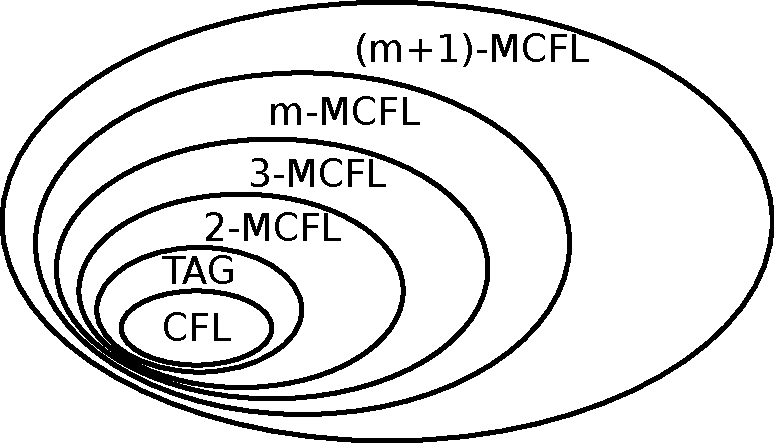
\includegraphics[width=\textwidth]{figures/mcfg/mcfg.pdf}
    \label{fig:mcfg_hierarachy_1}    
    \caption{Иерархия по $m$}
\end{figure}  

  Иерархия для $m=1$
 \begin{theorem}
  1-MCFL = CFL
 \end{theorem}

 \begin{theorem}
  1-MCFL(1) $\varsubsetneq$ 1-MCFL(2)
 \end{theorem}
 
 \begin{theorem}
  1-MCFL($r$) = 1-MCFL($r+1$), $r\geq2$
 \end{theorem}

 Иерархия для $m=2$
 \begin{theorem}[Ramow, Satta]
  2-MCFL(2) = 2-MCFL(3)
 \end{theorem}

 \begin{theorem}
 Если $m>2$ или $r>2$, то m-MCFL(r) $\varsubsetneq$ m-MCFL(r+1)
 \end{theorem}

\begin{figure}
    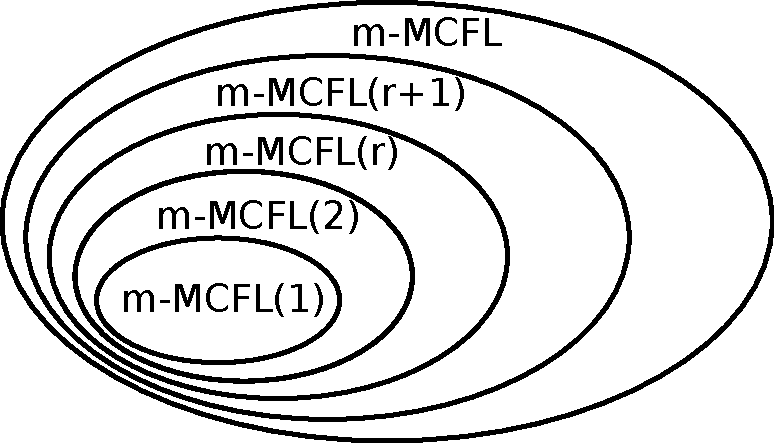
\includegraphics[width=\textwidth]{figures/mcfg/mcfg_2.pdf}
    \label{fig:mcfg_hierarachy_2}    
    \caption{Иерархия по $r$}
\end{figure}  


Про MIX и $O_n$

\begin{itemize}
    \item $mix = \{\omega \in \{a,b\}^* \mid |\omega|_a = |\omega|_b \}$ --- контекстно-свободный язык

    \item $MIX = \{\omega \in \{a,b,c\}^* \mid |\omega|_a = |\omega|_b = |\omega|_c\}$ --- MCFL? Хотелось верить, что нет
    \begin{itemize}
      \item \href{https://hal.inria.fr/inria-00564552/document}{MIX is a 2-MCFL and the word problem in $\mathbb{Z}^2$ is solved by a third-order collapsible pushdown automaton, Sylvain Salvati, 2011}~\cite{salvati:inria-00564552}
    \end{itemize}    
    \item $O_2=\{\omega \in \{a,\overline{a},b,\overline{b}\}^* \mid |\omega|_a=|\omega|_{\overline{a}} \wedge |w|_b=|w|_{\overline{b}}\}$
    \item $O_n=\{\omega \in \{a_1,\overline{a_1},a_2,\overline{a_2},\ldots,a_n,\overline{a_n}\}^* \mid |\omega|_{a_1}=|\omega|_{\overline{a_1}} \wedge |w|_{a_2}=|w|_{\overline{a_2}} \wedge \cdots \wedge |w|_{a_n}=|w|_{\overline{a_n}}\}$
    \item $MIX_n = \{\omega \in \{a_1,\ldots,a_n\}^* \mid |\omega|_{a_1} = |\omega|_{a_2} =\cdots = |\omega|_{a_n}\}$    
    \item $MIX_n$ регулярно эквивалентен $O_n$ (существует алгоритм построения грамматики одного языка по грамматике другого)
    \begin{itemize}
      \item \href{https://hal.archives-ouvertes.fr/hal-01771670/document}{$O_n$ is an n-MCFL, Sylvain Salvati, 2018}~\cite{GEBHARDT202241}
    \end{itemize}
  \end{itemize}
  

  \begin{itemize}
    \item Варианты леммы о накачке
    \item Представимость конкретных языков
    \begin{itemize}
      \item Многомерный язык Дика: \href{https://link.springer.com/chapter/10.1007/978-3-662-59620-3_5}{Towards a 2-Multiple Context-Free Grammar for the 3-Dimensional Dyck Language, Konstantinos Kogkalidis, Orestis Melkonian, 2019}~\cite{10.1007/978-3-662-59620-3_5}
      \item Шафл языков Дика: \href{https://dl.acm.org/doi/10.1145/3093333.3009848}{Context-sensitive data-dependence analysis via linear conjunctive language reachability, Qirun Zhang, Zhendong Su et al, 2017}~\cite{10.1145/3009837.3009848}
    \end{itemize}
  \end{itemize}  

 % FIXME: Переписать главу
% %\input{ConjunctiveAndBooleanLanguages}
\setchapterpreamble[u]{\margintoc}
\chapter[Пути с ограничениями в терминах формальных языков]{Задача о поиске путей с ограничениями в терминах формальных языков}
\label{chpt:FLPQ}
\tikzsetfigurename{FLPQ_}

В данной главе сформулируем постановку задачи о поиске путей в графе с ограничениями.
Также мы приведём несколько примеров областей, в которых применяются алгоритмы решения этой задачи.

\section{Постановка задачи}

Пусть нам дан конечный ориентированный помеченный граф $\mscrG = \langle V, E, L \rangle$.
Функция $\omega(\pi) = \omega((v_0, l_0, v_1), (v_1, l_1, v_2), \dots, (v_{n-1}, l_{n-1}, v_n)) = l_0 \cdot l_1 \cdot \dots \cdot l_{n-1}$ строит слово по пути посредством конкатенации меток рёбер вдоль этого пути.
Очевидно, для пустого пути данная функция будет возвращать пустое слово, а для пути длины $n  > 0$~--- непустое слово длины $n$.

Если теперь рассматривать задачу поиска путей, то окажется, что то множество путей, которое мы хотим найти, задаёт множество слов, то есть язык.
А значит, критерий поиска мы можем сформулировать следующим образом: нас интересуют такие пути, что слова, составленные из меток вдоль них, принадлежат заданному языку.

\begin{definition}[Задача поиска путей с ограничениями в терминах формальных языков]
    \label{def1}
    \emph{Задача поиска путей с ограничениями в терминах формальных языков} заключается в поиске множества путей $\Pi = \{\pi \mid \omega(\pi) \in \mscrL\}$.
\end{definition}

В задаче поиска путей мы можем накладывать дополнительные ограничения на путь (например, чтобы он был простым, кратчайшим или Эйлеровым~\sidecite{kupferman2016eulerian}), но это уже другая история.

Другим вариантом постановки задачи является задача достижимости.

\begin{definition}[Задача достижимости]
    \label{def2}
    \emph{Задача достижимости} заключается в поиске множества пар вершин, для которых найдется путь с началом и концом в этих вершинах, что слово, составленное из меток рёбер пути, будет принадлежать заданному языку
    \[\Pi' = \{(v_{i}, v_{j}) \mid \exists v_{i} \pi v_{j}, \omega(\pi) \in \mscrL\}.\]
\end{definition}

При этом, множество $\Pi$ может являться бесконечным, тогда как $\Pi'$ конечно, по причине конечности графа $\mscrG$.

Язык $\mscrL$ может принадлежать разным классам и быть задан разными способами.
Например, он может быть регулярным, контекстно-свободным, или многокомпонентным контекстно-свободным.

Если $\mscrL$~--- регулярный, $\mscrG$ можно рассматривать как недетерминированный конечный автомат (НКА), в котором все вершины являются одновременно и стартовыми, и конечными.
Тогда задача поиска путей, в которой $\mscrL$~--- регулярный, сводится к пересечению двух регулярных языков.

Более подробно мы рассмотрим случай, когда $\mscrL$~--- контекстно-свободный язык.

Путь $G = \langle \Sigma, N, P \rangle$~--- контекстно-свободная грамматика.
Будем считать, что $L \subseteq \Sigma$.
Мы не фиксируем стартовый нетерминал в определении грамматики, поэтому, чтобы описать язык, задаваемый ей, нам необходимо отдельно зафиксировать стартовый нетерминал.
Таким образом, будем говорить, что $L(G,N_i) = \{ w \mid N_i \xRightarrow[G]{*} w  \}$~--- это язык задаваемый грамматикой $G$ со стартовым нетерминалом $N_i$.

\begin{example}
    Пример задачи поиска путей.

    Дана грамматика $G$, задающая язык $\mscrL = a^n b^n$:
    \begin{align*}
        S & \to a b   \\
        S & \to a S b
    \end{align*}
    И дан граф $\mscrG$:
    \begin{center}
        \begin{tikzpicture}[]
  % Apex angle 60 degrees
  \node[isosceles triangle,
    isosceles triangle apex angle=60,
    draw=none,fill=none,
    minimum size=2cm] (T60) at (3,0){};


  \node[state] (q_0) at (T60.right corner) {$0$};
  \node[state] (q_1) at (T60.left corner)  {$1$};
  \node[state] (q_2) at (T60.apex)         {$2$};
  \node[state] (q_3) [right=1.5 of q_2]  {$3$};
  \path[->]
  (q_0) edge[left]  node {a} (q_1)
  (q_1) edge[above]  node {a} (q_2)
  (q_2) edge[below]  node {a} (q_0)
  (q_2) edge[bend left, above]  node {b} (q_3)
  (q_3) edge[bend left, below]  node {b} (q_2);
\end{tikzpicture}

    \end{center}

    Кратчайшими путями, принадлежащими множеству $\Pi = \{\pi \mid \omega(\pi) \in \mscrL\}$, являются:

    \begin{center}
        \input{figures/flpq/path1.tex}
    \end{center}

    \begin{center}
        \input{figures/flpq/path2.tex}
    \end{center}

\end{example}


\section{О разрешимости задачи}

Задачи из определения \ref{def1} и \ref{def2} сводятся к построению пересечения языка $\mscrL$ и языка, задаваемого путями графа, $R$.
А мы для обсуждения разрешимости задачи рассмотрим более слабую постановку задачи:

\begin{definition}[TODO: Что ты?]
    Необходимо проверить, что существует хотя бы один такой путь $\pi$ для данного графа, для данного языка $\mscrL$, что $\omega(\pi) \in \mscrL$.
\end{definition}

Эта задача сводится к проверке пустоты пересечения языка $\mscrL$ c $R$~--- регулярным языком, задаваемым графом.
От класса языка $\mscrL$ зависит её разрешимость:
\begin{itemize}
    \item Если $\mscrL$ регулярный, то получаем задачу пересечения двух регулярных языков: $\mscrL \cap R = R'$.
          $R'$~--- также регулярный язык.
          Проверка регулярного языка на пустоту~--- разрешимая проблема.
    \item Если $\mscrL$ контекстно-свободный, то получаем задачу: $\mscrL \cap R = CF$~--- контекстно-свободный.
          Проверка контекстно-свободного языка на пустоту~--- разрешимая проблема.
    \item Помимо иерархии Хомского существуют и другие классификации языков.
          Так например, класс конъюнктивных (Conj) языков~\sidecite{DBLP:journals/jalc/Okhotin01}является строгим расширением контекстно-свободных языков и все так же позволяет полиномиальный синтаксический анализ.

          Пусть $\mscrL$~--- конъюнктивный.
          При пересечении конъюнктивного и регулярного языков получается конъюнктивный ($\mscrL \cap R = Conj$), а проблема проверки Conj на пустоту не разрешима~\sidecite{DBLP:journals/tcs/Okhotin03a}.
    \item Ещё один класс языков из альтернативной иерархии, не сравнимой с Иерархией Хомского,~--- MCFG (multiple context-free grammars)~\sidecite{SEKI1991191}.
          Как его частный случай~--- TAG (tree adjoining grammar)~\sidecite{Joshi1997}.

          Если $\mscrL$ принадлежит классу MCFG, то $\mscrL \cap R$ также принадлежит MCFG.
          Проблема проверки пустоты MCFG разрешима~\sidecite{SEKI1991191}.
\end{itemize}

Существует ещё много других классификаций языков, но поиск универсальной иерархии до сих пор продолжается.

Далее, для изучения алгоритмов решения, нас будет интересовать задача $R \cap CF$.

\section{Области применения}

Поиск путей с ограничениями в виде формальных языков широко применяется в различных областях.
Ниже даны ключевые работы по применению поиска путей с контекстно-свободными ограничениями и ссылки на них для более детального ознакомления.
\begin{itemize}
    \item Межпроцедурный Статанализ кода.
          Идея начала активно разрабатываться Томасом Репсом~\sidecite{Reps}.
          Далее последовал ряд, в том числе инженерных работ, применяющих достижимость с контекстно-свободными ограничениями для анализа указателей, анализа алиасов и других прикладных задач~\sidecite{LabelFlowCFLReachability,specificationCFLReachability,Zheng}.
    \item Графовые БД.
          Впервые задача сформулирована Михалисом Яннакакисом~\sidecite{Yannakakis}.
          Запросы с контекстно-свободными ограничениями нашли своё применение различных областях.
          \begin{itemize}
              \item Социальные сети~\sidecite{Hellings2015PathRF}.
              \item RDF обработка~\sidecite{10.1007/978-3-319-46523-4_38}.
              \item Биоинформатика~\sidecite{cfpqBio}.
          \end{itemize}
\end{itemize}

%\begin{itemize}
%    \item OpenCypher~\cite{Kuijpers:2019:ESC:3335783.3335791}
%    \item J.Hellings. CFPQ~\cite{hellingsRelational,hellings2015querying,Hellings2015PathRF}
%    \item Zhang. CFPQ on rdf graphs~\cite{10.1007/978-3-319-46523-4_38}
%    \item Bradford~\cite{bradford2007quickest,ward2008distributed,bradford2016fast,Bradford:2008:LCG:1373936.1373946}
%\end{itemize}


%\section{Вопросы и задачи}
%\begin{enumerate}
%    \item Пусть есть граф. Задайте грамматику для поиска всех путей, таких, что....
%    \item Существует ли в графе !!! путь из А в Б, такой что!!!
%    \item Для графа !!! постройте все пути, удовлетворяющие !!!!
%
%    \item Задача 1
%    \item Задача 2
%\end{enumerate}

\setchapterpreamble[u]{\margintoc}
\chapter{Поиск путей с регулярными ограничениями}
\tikzsetfigurename{RPQ_}

\section{Достижимость между всеми парами вершин}

Через тензорное произведение.

Классическое построение пересечения автоматов строит их тензорное произведение.

Так как мы хотим отвечать ещё и на вопрос о достижимости, что нам надо ещё и транзитивное замыкание посчитать.

\section{Достижимость с несколькими источниками}

Достижимость от нескольких стартовых вершин через обход в ширину, основанный на линейной алгебре~\sidecite{9286186}.

Идея алгоритма основана на одновременном обходе в ширину графа и конечного автомата, построенного по грамматике.

В классической версии обхода в ширину, основанного на линейной алгебре, используется вектор, куда записывается фронт обхода графа.
Так, один раз перемножая этот вектор на матрицу смежности графа, можно совершать один шаг в обходе графа.
Покажем на примере, как данный метод может быть использован, когда мы накладываем дополнительные ограничения в виде регулярного языка на путь в графе.

Для этого, во-первых, предъявим булевые представления для матриц смежности графа и автомата для регулярного языка.
Затем, введем специальную блочно-диагональную матрицу для синхронизации обхода в ширину по двум матрицам смежности.
Далее, попробуем наивно реализовать обход в ширину, и посмотрим, почему наивная реализация может выдавать некорректный результат.
После этого перейдем к реализации обхода в ширину более продвинутым методом, который решает проблему наивного подхода.

\subsection{Пример работы алгоритма}
\marginnote{TODO: Подумать над разбиением на разделы и подразделы}
Возьмём следующий граф.
\begin{center}
    \label{input_rpq}
    \begin{tikzpicture}[node distance=2cm,shorten >=1pt,on grid,auto]
        \node[state] (q_0)   {$1$};
        \node[state] (q_1) [above=of q_0] {$2$};
        \node[state] (q_2) [right=of $(q_0)!0.5!(q_1)$] {$0$};
        \node[state] (q_3) [right=of q_2] {$3$};
        \path[->]
        (q_0) edge  node {b} (q_1)
        (q_1) edge  node[pos=0.3] {a} (q_2)
        (q_2) edge  node[pos=0.7] {a} (q_0)
        (q_2) edge[bend left]  node[above] {b} (q_3)
        (q_3) edge[bend left]  node {b} (q_2);
    \end{tikzpicture}
\end{center}

Его матрица смежности имеет следующий вид.
\marginnote{TODO: Точка внизу или снизу?}
\[
    G_1 =
    \begin{pmatrix}
        .     & \{a\} & .     & \{b\} \\
        .     & .     & \{b\} & .     \\
        \{a\} & .     & .     & .     \\
        \{b\} & .     & .     & .
    \end{pmatrix}
    \qquad
    G_1 =
    \begin{pmatrix}
        \cdot & \{a\} & \cdot & \{b\} \\
        \cdot & \cdot & \{b\} & \cdot \\
        \{a\} & \cdot & \cdot & \cdot \\
        \{b\} & \cdot & \cdot & \cdot
    \end{pmatrix}
\]

Её булева декомпозиция по каждому символу выглядит следующим образом.
\[
    G_{0\_a} = \begin{pmatrix}
        0 & 1 & 0 & 0 \\
        0 & 0 & 0 & 0 \\
        1 & 0 & 0 & 0 \\
        0 & 0 & 0 & 0 \\
    \end{pmatrix} \qquad
    G_{0\_b} = \begin{pmatrix}
        0 & 0 & 0 & 1 \\
        0 & 0 & 1 & 0 \\
        0 & 0 & 0 & 0 \\
        1 & 0 & 0 & 0 \\
    \end{pmatrix}
\]

Зададим ограничения с помощью регулярного выражения $b^*ab$, которое представляется автоматом из трех последовательных состояний.
\begin{center}
    \begin{tikzpicture}[shorten >=1pt,on grid,auto]
        \node[state, initial]   (q_0) at (0,0)  {$0$};
        \node[state]             (q_1) at (2,0)  {$1$};
        \node[state, accepting] (q_2) at (4,0)  {$2$};
        \path[->]
        (q_0) edge  node {$a$} (q_1)
        (q_1) edge  node {$b$} (q_2);
        \draw (q_0) edge[loop above]  node {$b$} (q_0);
    \end{tikzpicture}
\end{center}

Автомат может быть задан матрицей смежности (с дополнительной информацией о стартовых и финальных состояниях).

Для регулярного выражения $b^*ab$ матрица смежности выглядит следующим образом (при этом нужно запомнить, что состояние $0$ является начальным, $2$~--- конечным).
\[
    G_2 =
    \begin{pmatrix}
        \{b\} & \{a\} & .     \\
        .     & .     & \{b\} \\
        .     & .     & .
    \end{pmatrix}
\]

Нам будет необходима булева декомпозиция этой матрицы, и она выглядит следующим образом.
\[
    R_{0\_a} = \begin{pmatrix}
        0 & 1 & 0 \\
        0 & 0 & 0 \\
        0 & 0 & 0
    \end{pmatrix} \qquad
    R_{0\_b} = \begin{pmatrix}
        1 & 0 & 0 \\
        0 & 0 & 1 \\
        0 & 0 & 0
    \end{pmatrix}
\]

\NewDocumentCommand{\MDa}{}{\begin{pNiceArray}[margin]{ccc|cccc}
        0 & 1 & 0 & 0 & 0 & 0 & 0 \\
        0 & 0 & 0 & 0 & 0 & 0 & 0 \\
        0 & 0 & 0 & 0 & 0 & 0 & 0 \\
        \midrule
        0 & 0 & 0 & 0 & 1 & 0 & 0 \\
        0 & 0 & 0 & 0 & 0 & 0 & 0 \\
        0 & 0 & 0 & 1 & 0 & 0 & 0 \\
        0 & 0 & 0 & 0 & 0 & 0 & 0
    \end{pNiceArray}}
\NewDocumentCommand{\MDb}{}{\begin{pNiceArray}[margin]{ccc|cccc}
        1 & 0 & 0 & 0 & 0 & 0 & 0 \\
        0 & 0 & 1 & 0 & 0 & 0 & 0 \\
        0 & 0 & 0 & 0 & 0 & 0 & 0 \\
        \midrule
        0 & 0 & 0 & 0 & 0 & 0 & 1 \\
        0 & 0 & 0 & 0 & 0 & 1 & 0 \\
        0 & 0 & 0 & 0 & 0 & 0 & 0 \\
        0 & 0 & 0 & 1 & 0 & 0 & 0
    \end{pNiceArray}}

Для синхронизации обхода составим набор блочно-диагональных матриц, каждая из которых~--- это прямая сумма двух матриц: $D_{0\_a} = R_{0\_a} \oplus G_{0\_a}$ и $D_{0\_a} = R_{0\_b} \oplus G_{0\_b}$.
\[
    D_{0\_a} = \MDa \quad
    D_{0\_b} = \MDb
\]

Пусть мы решаем частный случай задачи достижимости с несколькими стартовыми вершинами (multiple-source)~--- достижимость с одной стартовой вершиной (single-source).

Пусть единственной начальной вершиной в графе будет вершина $0$.

Теперь создадим вектор
$v = \begin{pNiceArray}[]{ccc|cccc}
        1 & 0 & 0 & 1 & 0 & 0 & 0
    \end{pNiceArray}$,
где в первой части стоит единица на месте начального состояния $0$ в автомате.
Во второй части содержится фронт обхода графа, на первом шаге это всегда множество стартовых вершин.
В данном случае единица стоит на месте единственной стартовой вершины~--- $0$.

Совершим один шаг в обходе графа и получим новый фронт обхода графа.
\begin{widepar}
    \begin{gather*}
        a: \begin{pNiceArray}[]{ccc|cccc}
            1 & 0 & 0 & 1 & 0 & 0 & 0
        \end{pNiceArray} \cdot \MDa =
        \begin{pNiceArray}[]{ccc|cccc}
            0 & 1 & 0 & 0 & 1 & 0 & 0
        \end{pNiceArray}
        \\
        b: \begin{pNiceArray}[]{ccc|cccc}
            1 & 0 & 0 & 1 & 0 & 0 & 0
        \end{pNiceArray} \cdot \MDb  =
        \begin{pNiceArray}[]{ccc|cccc}
            1 & 0 & 0 & 0 & 0 & 0 & 1
        \end{pNiceArray}
    \end{gather*}
\end{widepar}

Сложим два полученных вектора, чтобы получить новый фронт обхода графа:
\begin{widepar}
    \[
        \begin{pNiceArray}[]{ccc|cccc}
            0 & 1 & 0 & 0 & 1 & 0 & 0
        \end{pNiceArray} +
        \begin{pNiceArray}[]{ccc|cccc}
            1 & 0 & 0 & 0 & 0 & 0 & 1
        \end{pNiceArray} =
        \begin{pNiceArray}[]{ccc|cccc}
            1 & 1 & 0 & 0 & 1 & 0 & 1
        \end{pNiceArray}.
    \]
\end{widepar}

То есть в наш фронт
$\begin{pmatrix}
        0 & 1 & 0 & 1
    \end{pmatrix}$
попали вершины 1 и 3 соотвественно.
А именно, мы совершили следующие переходы в графе и автомате.

\begin{minipage}{0.45\textwidth}
    \begin{center}
        \begin{tikzpicture}[node distance=2cm,shorten >=1pt,on grid,auto]
            \node[state, red] (q_0)   {$1$};
            \node[state] (q_1) [above=of q_0] {$2$};
            \node[state] (q_2) [right=of $(q_0)!0.5!(q_1)$] {$0$};
            \node[state, red] (q_3) [right=of q_2] {$3$};
            \path[->, red]
            (q_2) edge  node[pos=0.7] {a} (q_0)
            (q_2) edge[bend left]  node[above] {b} (q_3);
            \path[->]
            (q_0) edge  node {b} (q_1)
            (q_1) edge  node[pos=0.3] {a} (q_2)
            (q_3) edge[bend left]  node {b} (q_2);
        \end{tikzpicture}
    \end{center}
\end{minipage}
\begin{minipage}{0.45\textwidth}
    \begin{center}
        \begin{tikzpicture}[shorten >=1pt,on grid,auto]
            \node[state, draw=none]      (q_3) at (0,0)  {$ $}; % empty node for alignment
            \node[state, initial, red]   (q_0) at (0,1)  {$0$};
            \node[state, red]            (q_1) at (2,1)  {$1$};
            \node[state, accepting]      (q_2) at (4,1)  {$2$};
            \path[->, red]
            (q_0) edge  node {$a$} (q_1);
            \path[->]
            (q_1) edge  node {$b$} (q_2);
            \draw (q_0) edge[loop above, red]  node {$b$} (q_0);
        \end{tikzpicture}
    \end{center}
\end{minipage}

Совершим еще один шаг алгоритма.
Теперь вектор $v$, на который мы умножаем матрицы, имеет следующий вид
$\begin{pNiceArray}[]{ccc|cccc}
        1 & 1 & 0 & 0 & 1 & 0 & 1
    \end{pNiceArray}$.
\begin{widepar}
    \begin{gather*}
        a: \begin{pNiceArray}[]{ccc|cccc}
            1 & 1 & 0 & 0 & 1 & 0 & 1
        \end{pNiceArray} \cdot \MDa =
        \begin{pNiceArray}[]{ccc|cccc}
            0 & 1 & 0 & 0 & 0 & 0 & 0
        \end{pNiceArray} \displaybreak[0] \\ % FIXME: remove \displaybreak[0]
        b: \begin{pNiceArray}[]{ccc|cccc}
            1 & 1 & 0 & 0 & 1 & 0 & 1
        \end{pNiceArray} \cdot \MDb =
        \begin{pNiceArray}[]{ccc|cccc}
            1 & 0 & 1 & 1 & 0 & 1 & 0
        \end{pNiceArray} \\
        \begin{pNiceArray}[]{ccc|cccc}
            0 & 1 & 0 & 0 & 0 & 0 & 0
        \end{pNiceArray} +
        \begin{pNiceArray}[]{ccc|cccc}
            1 & 0 & 1 & 1 & 0 & 1 & 0
        \end{pNiceArray} =
        \begin{pNiceArray}[]{ccc|cccc}
            1 & 1 & 1 & 1 & 0 & 1 & 0
        \end{pNiceArray}
    \end{gather*}
\end{widepar}
То есть в наш фронт
$\begin{pmatrix}
        1 & 0 & 1 & 0
    \end{pmatrix}$
попали вершины 0 и 2 соотвественно.
Мы совершили следующие переходы в графе и автомате.

\begin{minipage}{0.45\textwidth}
    \begin{center}
        \begin{tikzpicture}[node distance=2cm,shorten >=1pt,on grid,auto]
            \node[state, gray] (q_0)   {$1$};
            \node[state, teal] (q_1) [above=of q_0] {$2$};
            \node[state, teal] (q_2) [right=of $(q_0)!0.5!(q_1)$] {$0$};
            \node[state, gray] (q_3) [right=of q_2] {$3$};
            \path[->, gray]
            (q_2) edge  node[pos=0.7] {a} (q_0)
            (q_2) edge[bend left]  node[above] {b} (q_3);
            \path[->, red]
            (q_0) edge  node {b} (q_1)
            (q_3) edge[bend left]  node {b} (q_2);
            \path[->]
            (q_1) edge  node[pos=0.3] {a} (q_2);
        \end{tikzpicture}
    \end{center}
\end{minipage}
\begin{minipage}{0.45\textwidth}
    \begin{center}
        \begin{tikzpicture}[shorten >=1pt,on grid,auto]
            \node[state, draw=none]            (q_3) at (0,0)  {$ $}; % empty node for alignment
            \node[state, initial, red]         (q_0) at (0,1)  {$0$};
            \node[state, gray]                 (q_1) at (2,1)  {$1$};
            \node[state, accepting, teal]      (q_2) at (4,1)  {$2$};
            \path[->, gray]
            (q_0) edge  node {$a$} (q_1);
            \path[->, red]
            (q_1) edge  node {$b$} (q_2);
            \draw (q_0) edge[loop above, red]  node {$b$} (q_0);
        \end{tikzpicture}
    \end{center}
\end{minipage}

При этом, можно заметить, что мы достигли конечной вершины в автомате.
Последний элемент левой части результирующего вектора
$\begin{pNiceArray}[]{ccc|cccc}
        1 & 1 & \textcolor{red}{1} & 1 & 0 & 1 & 0
    \end{pNiceArray}$
отвечает за состояние 2, которое является конечным.
А значит, обход необходимо остановить, и текущие вершины фронта обхода графа записать в ответ.

Таким образом, вершины графа 0 и 2 являются ответом.
Однако вершина 0~--- лишняя.
Регулярное выражение $b^*ab$ не подразумевает, что вершина 0 в графе может быть достигнута.
Она могла бы быть достигнута по пустой строке в случае, если бы регулярное выражение имело вид $b^*$ или по строке $aba$ в случае, если бы регулярное выражение имело вид $b^*aba$.

Это произошло, потому что в векторе $v$ должна кодироваться информация о паре~--- вершине графа и состоянии автомата.
Достигнув вершины 0, мы оказались в конечном состоянии автомата, которое было получено с помощью другой вершины~--- вершины 2.

Эту проблему можно решить, закодировав информацию о каждой такой паре в несколько векторов $v$, и ограничив левую часть вектора $v$ таким образом, чтобы в ней всегда была лишь одна единица.

Тогда мы получим, что вектор $v$ вида
$\begin{pNiceArray}[]{ccc|cccc}
        1 & 0 & 0 & 1 & 0 & 1 & 0
    \end{pNiceArray}$
будет хранить информацию о парах $(0, 0)$ и $(0, 2)$, где первый элемент пары~--- состояние автомата, а второй~--- вершина графа.

Аналогично, вектор $v$ вида
$\begin{pNiceArray}[]{ccc|cccc}
        0 & 1 & 0 & 0 & 1 & 1 & 0
    \end{pNiceArray}$
кодирует информацию о парах $(1, 1)$ и $(1, 2)$.
Вектор $v$ вида
$\begin{pNiceArray}[]{ccc|cccc}
        0 & 0 & 1 & 0 & 0 & 1 & 1
    \end{pNiceArray}$
кодирует информацию о парах $(2, 2)$ и $(2, 3)$.

Таким образом, мы будем понимать, в каком состоянии автомата мы находимся для каждой из вершин фронта обхода графа.

Рассмотрим, как это применяется в разработанном алгоритме, который представлен далее.

Предлагается \enquote{расклеить} $v$ в матрицу $M$, состоящую из трех векторов, добавив два вектора $\begin{pNiceArray}[]{ccc|cccc}
        0 & 1 & 0 & 0 & 0 & 0 & 0
    \end{pNiceArray}$
и $\begin{pNiceArray}[]{ccc|cccc}
        0 & 0 & 1 & 0 & 0 & 0 & 0
    \end{pNiceArray}$.
Во второй части этих векторов стоят нули, так как
$\begin{pmatrix}
        0 & 1 & 0
    \end{pmatrix}$
и
$\begin{pmatrix}
        0 & 0 & 1
    \end{pmatrix}$
кодируют состояния автомата 1 и 2, которые не являются начальными.
\NewDocumentCommand{\MMf}{}{\begin{pNiceArray}[]{ccc|cccc}
        1 & 0 & 0 & 1 & 0 & 0 & 0 \\
        0 & 1 & 0 & 0 & 0 & 0 & 0 \\
        0 & 0 & 1 & 0 & 0 & 0 & 0
    \end{pNiceArray}}
\[M = \MMf\]

И совершать обход тем же самым образом, но сохранив с помощью матрицы $M$ дополнительную информацию о парах (состояние, вершина).
\begin{widepar}
    \begin{gather*}
        a: \MMf \cdot \MDa = \begin{pNiceArray}[]{ccc|cccc}
            0 & 1 & 0 & 0 & 1 & 0 & 0 \\
            0 & 0 & 0 & 0 & 0 & 0 & 0 \\
            0 & 0 & 0 & 0 & 0 & 0 & 0
        \end{pNiceArray} \\
        b: \MMf \cdot \MDb = \begin{pNiceArray}[]{ccc|cccc}
            1 & 0 & 0 & 0 & 0 & 0 & 1 \\
            0 & 0 & 1 & 0 & 0 & 0 & 0 \\
            0 & 0 & 0 & 0 & 0 & 0 & 0
        \end{pNiceArray}
    \end{gather*}
\end{widepar}

Для того, чтобы левая часть матрицы $M$ всегда оставалось единичной, нужно трансформировать в ней строчки особым образом.
Для этого нужно складывать только те вектора в правой части матрицы $M$, у которых в левой части единицы стоят на одинаковых позициях.
После чего переставлять строчки в $M$ так, чтобы левая часть матрицы $M$ принимала единичный вид.
Вектора с пустой левой частью нас при этом не интересуют.

Тогда правая часть матрицы $M$ будет кодировать текущий фронт обхода графа.

В нашем примере матрица $M$ для следующего шага обхода выглядит следующим образом.
\NewDocumentCommand{\MMs}{}{\begin{pNiceArray}[]{ccc|cccc}
        1 & 0 & 0 & 0 & 0 & 0 & 1 \\
        0 & 1 & 0 & 0 & 1 & 0 & 0 \\
        0 & 0 & 1 & 0 & 0 & 0 & 0
    \end{pNiceArray}}
\[M = \MMs\]

Видно, что во фронт обхода графа попали вершины 1 и 3.
В вершину 1 мы попали в состоянии 1, в вершину 3~--- в состоянии 0.

Совершаются следующие переходы в графе и автомате.

\begin{minipage}{0.45\textwidth}
    \begin{center}
        \begin{tikzpicture}[node distance=2cm,shorten >=1pt,on grid,auto]
            \node[state, red] (q_0)   {$1$};
            \node[state] (q_1) [above=of q_0] {$2$};
            \node[state] (q_2) [right=of $(q_0)!0.5!(q_1)$] {$0$};
            \node[state, red] (q_3) [right=of q_2] {$3$};
            \path[->, red]
            (q_2) edge  node[pos=0.7] {a} (q_0)
            (q_2) edge[bend left]  node[above] {b} (q_3);
            \path[->]
            (q_0) edge  node {b} (q_1)
            (q_1) edge  node[pos=0.3] {a} (q_2)
            (q_3) edge[bend left]  node {b} (q_2);
        \end{tikzpicture}
    \end{center}
\end{minipage}
\begin{minipage}{0.45\textwidth}
    \begin{center}
        \begin{tikzpicture}[shorten >=1pt,on grid,auto]
            \node[state, draw=none]      (q_3) at (0,0)  {$ $}; % empty node for alignment
            \node[state, initial, red]   (q_0) at (0,1)  {$0$};
            \node[state, red]            (q_1) at (2,1)  {$1$};
            \node[state, accepting]      (q_2) at (4,1)  {$2$};
            \path[->, red]
            (q_0) edge  node {$a$} (q_1);
            \path[->]
            (q_1) edge  node {$b$} (q_2);
            \draw (q_0) edge[loop above, red]  node {$b$} (q_0);
        \end{tikzpicture}
    \end{center}
\end{minipage}

Сделаем еще один шаг алгоритма и придем к конечному состоянию в автомате.
\NewDocumentCommand{\MMt}{}{\begin{pNiceArray}[]{ccc|cccc}
        1 & 0 & 0 & 1 & 0 & 0 & 0 \\
        0 & 1 & 0 & 0 & 0 & 0 & 0 \\
        0 & 0 & 1 & 0 & 0 & 1 & 0
    \end{pNiceArray}}

\begin{widepar}
    \begin{gather*}
        \MMs \cdot \MDa = \begin{pNiceArray}[]{ccc|cccc}
            0 & 1 & 0 & 0 & 0 & 0 & 0 \\
            0 & 0 & 0 & 0 & 0 & 0 & 0 \\
            0 & 0 & 0 & 0 & 0 & 0 & 0
        \end{pNiceArray} \\
        \MMs \cdot \MDb = \begin{pNiceArray}[]{ccc|cccc}
            1 & 0 & 0 & 1 & 0 & 0 & 0 \\
            0 & 0 & 1 & 0 & 0 & 1 & 0 \\
            0 & 0 & 0 & 0 & 0 & 0 & 0
        \end{pNiceArray} \\
        M = \MMt
    \end{gather*}
\end{widepar}

Видно, что мы достигли вершины 2 графа в конечном состоянии 2 автомата.
При этом вершина 0 графа так же достигнута, как и в наивном варианте алгоритма, но теперь известно, что это происходит в состоянии 0 автомата.

\begin{minipage}{0.45\textwidth}
    \begin{center}
        \begin{tikzpicture}[node distance=2cm,shorten >=1pt,on grid,auto]
            \node[state, gray] (q_0)   {$1$};
            \node[state, teal] (q_1) [above=of q_0] {$2$};
            \node[state, red] (q_2) [right=of $(q_0)!0.5!(q_1)$] {$0$};
            \node[state, gray] (q_3) [right=of q_2] {$3$};
            \path[->, gray]
            (q_2) edge  node[pos=0.7] {a} (q_0)
            (q_2) edge[bend left]  node[above] {b} (q_3);
            \path[->, red]
            (q_0) edge  node {b} (q_1)
            (q_3) edge[bend left]  node {b} (q_2);
            \path[->]
            (q_1) edge  node[pos=0.3] {a} (q_2);
        \end{tikzpicture}
    \end{center}
\end{minipage}
\begin{minipage}{0.45\textwidth}
    \begin{center}
        \begin{tikzpicture}[shorten >=1pt,on grid,auto]
            \node[state, draw=none]            (q_3) at (0,0)  {$ $}; % empty node for alignment
            \node[state, initial, red]         (q_0) at (0,1)  {$0$};
            \node[state, gray]                 (q_1) at (2,1)  {$1$};
            \node[state, accepting, teal]      (q_2) at (4,1)  {$2$};
            \path[->, gray]
            (q_0) edge  node {$a$} (q_1);
            \path[->, red]
            (q_1) edge  node {$b$} (q_2);
            \draw (q_0) edge[loop above, red]  node {$b$} (q_0);
        \end{tikzpicture}
    \end{center}
\end{minipage}

Таким образом, в ответ попадает вершина 2.

Перейдем к формальному описанию алгоритма.

\subsection{Формальное описание алгоритма}

Алгоритм принимает на вход граф $\mscrG$, детерминированный конечный автомат $\mscrR$, описывающий регулярную грамматику, и множество начальных вершин $V_{\mathrm{src}}$ графа.

Граф $\mscrG$ и автомат $\mscrR$ можно представить в виде булевых матриц смежности.
Так, в виде словаря для каждой метки графа заводится булева матрица смежности, на месте $(i, j)$ ячейки которой стоит 1, если $i$ и $j$ вершины графа соединены ребром данной метки.
Такая же операция проводится для автомата грамматики $\mscrR$.

Далее, мы оперируем с двумя словарями, где ключом является символ метки ребра графа или символ алфавита автомата, а значением~--- соответствующая им булевая матрица.

Для каждого символа из пересечения этих множеств строится матрица $\mfrakD$, как прямая сумма булевых матриц.
То есть, строится матрица $\mfrakD = \mathrm{Bool}_{\mscrR_a} \oplus \mathrm{Bool}_{\mscrG_a}$, которая определяется как
\[
    \mfrakD = \begin{pmatrix}
        \mathrm{Bool}_{\mscrR_a} & 0                        \\
        0                        & \mathrm{Bool}_{\mscrG_a}
    \end{pmatrix},
\]
где $\mscrR_{a}$ и $\mscrG_{a}$ матрицы смежности соответствующих символов автомата грамматики $\mscrR$ и графа $\mscrG$ для символа $a \in A_\mscrR \cap A_\mscrG$, $A_\mscrR \cap A_\mscrG$~--- пересечение алфавитов.
Такая конструкция позволяет синхронизировать алгоритм обхода в ширину одновременно для графа и грамматики.

Далее вводится матрица $M$, хранящая информацию о фронте обхода графа.
\marginnote{TODO: Надо подумать над обозначениями. Почему $Id$, а не $E$? Может быть вообще надо эти обозначения вводить сразу в примере.}
Она нужна для выделения множества пройденных вершин и не допускает зацикливание алгоритма.
\[
    M^{k \times (k + n)} = \begin{pNiceArray}[]{c|c}
        Id_k & Matrix_{k \times n }
    \end{pNiceArray},
\]
где $Id_k$~--- единичная матрица размера $k$, $k$~--- количество вершин в автомате $\mscrR$, $Matrix_{k \times n }$~--- матрица, хранящая в себе маску пройденных вершин в автомате графа, $n$~--- количество вершин в графе $\mscrG$.

\subsection{Выходные данные}

На выходе строится множество $\mscrP$ пар вершин $(v, w)$ графа $\mscrG$ таких, что вершина $w$ достижима из множества начальных вершин, при этом $v \in V_{\mathrm{src}}$, $w \not\in V_{\mathrm{src}}$.
Это множество представляется в виде матрицы размера $|V| \times |V|$, где $(i,j)$ ячейка содержит 1, если пара вершин с индексами $(i, j) \in \mscrP$.

\subsection{Процесс обхода графа}

Алгоритм обхода заключается в последовательном умножении матрицы $M$ текущего фронта на матрицу $\mfrakD$.
В результате чего, находится матрица $M'$ содержащая информацию о вершинах, достижимых на следующем шаге.
Далее, с помощью операций перестановки и сложения векторов $M'$ преобразуется к виду матрицы $M$ и присваивается ей.
Итерации продолжаются пока $M'$ содержит новые вершины, не содержащиеся в $M$. На листинге~\ref{BFSRPQ1} представлен этот алгоритм.

% \begin{algorithm}[t]
%     \caption{Алгоритм достижимости в графе с регулярными ограничениями на основе поиска в ширину, выраженный с помощью операций матричного умножения}\label{BFSRPQ1}
%     \begin{algorithmic}[1]
%         \Procedure{BFSBasedRPQ}{$\mscrR=\langle Q, \Sigma, P, F, q \rangle,\mscrG=\langle V, E, L \rangle, V_{\mathrm{src}}$}
%         \State $\mscrP\gets~${Матрица смежности графа}
%         \State $\mfrakD\gets \mathrm{Bool}_\mscrR \bigoplus \mathrm{Bool}_\mscrG$\Comment{Построение матриц $\mfrakD$}
%         \State $M\gets CreateMasks(|Q|,|V|)$ \Comment{Построение матрицы $M$}
%         \State $M'\gets SetStartVerts(M, V_{\mathrm{src}})$  \Comment{Заполнение нач. вершин}

%         \While{Матрица~$M$~меняется}{}
%         \State $M\gets M'\langle\neg M\rangle$\Comment{Применение комплементарной маски}
%         \ForAll{$a\in (\Sigma \cap L)$}
%         \State $M'\gets M~$any.pair$~\mfrakD$
%         \Comment{Матр. умножение в полукольце}
%         \State $M'\gets TransformRows(M')$\label{TransformRows}
%         \Comment{Приведение $M'$ к виду $M$}
%         \EndFor
%         \State {$Matrix\gets extractRightSubMatrix(M')$}
%         \State $V\gets Matrix.reduceVector()$ \Comment{Сложение по столбцам}
%         \For{$k \in 0\dots|V_{\mathrm{src}}|-1$}
%         \State $W\gets\mscrP.getRow(k)$
%         \State $\mscrP.setRow(k, V+W)$
%         \EndFor
%         \EndWhile
%         \State \textbf{return} $\mscrP$
%         \EndProcedure
%     \end{algorithmic}
% \end{algorithm}

В алгоритме~\ref{BFSRPQ1}, в~\ref{TransformRows} строке происходит трансформация строчек в матрице $M'$.
Это делается для того, чтобы представить полученную во время обхода матрицу $M'$, содержащую новый фронт, в виде матрицы $M$.
Для этого требуется так переставить строчки $M'$, чтобы она содержала корректные по своему определению значения.
То есть, имела единицы на главной диагонали, а все остальные значения в первых $k$ столбцах были нулями.
Подробнее эта процедура описана в листинге~\ref{AlgoTransformRows}.

% \begin{algorithm}[H]
%     \caption{Алгоритм трансформации строчек}\label{AlgoTransformRows}
%     \begin{algorithmic}[1]
%         \Procedure{TransformRows}{$M$}
%         \State{$T \gets extractLeftSubMatrix(M)$}
%         \State{$Ix, Iy \gets$ итераторы по индексам ненулевых элементов $T$}
%         \For{$i \in 0\dots|Iy|$}
%         \State{$R\gets M.getRow(Ix[i])$}
%         \State{$M'.setRow(Iy[i], R + M'.getRow(Iy[i]))$}
%         \EndFor
%         \EndProcedure
%     \end{algorithmic}
% \end{algorithm}

\subsection{Модификации алгоритма}

Рассмотрим $V_{\mathrm{src}}$~--- множество начальных вершин, состоящее из $r$ элементов.
Для каждой начальной вершины $V_{\mathrm{src}}^i \in V_{\mathrm{src}}$ отметим соответствующие индексы в матрице $M$ единицами, получив матрицу $M(V_{\mathrm{src}}^i)$, и построим матрицу $\mfrakM$ следующим образом.
\[
    \mfrakM^{(k*r) \times (k + n)} = \begin{pmatrix}
        M(V_{\mathrm{src}}^1) \\
        M(V_{\mathrm{src}}^2) \\
        M(\dots)              \\
        M(V_{\mathrm{src}}^r)
    \end{pmatrix}
\]

Матрица $\mfrakM$ собирается из множества матриц $M(V_{\mathrm{src}}^i)$ и позволяет хранить информацию о том, из какой начальной вершины достигаются новые вершины во время обхода.

% \begin{algorithm}[t]
%     \caption{Модификация алгоритма для поиска конкретной исходной вершины}\label{BFSRPQ2}
%     \begin{algorithmic}[1]
%         \Procedure{BFSBasedRPQ}{$\mscrR=\langle Q, \Sigma, P, F, q \rangle,\mscrG=\langle V, E, L \rangle, V_{\mathrm{src}}$}
%         \State $\mscrP\gets~${Матрица смежности графа}
%         \State $\mfrakD\gets \mathrm{Bool}_\mscrR \bigoplus \mathrm{Bool}_\mscrG$
%         \State $\mfrakM\gets CreateMasks(|Q|,|V|)$
%         \State $\mfrakM'\gets SetStartVerts(\mfrakM, V_{\mathrm{src}})$

%         \While{Матрица~$\mfrakM$~меняется}{}
%         \State $\mfrakM\gets \mfrakM'\langle\neg\mfrakM\rangle$
%         \ForAll{$a\in (\Sigma \cap L)$}
%         \State $\mfrakM'\gets \mfrakM~$any.pair$~\mfrakD$
%         \ForAll{$M \in \mfrakM'$}
%         \State $M\gets TransformRows(M)$
%         \EndFor
%         \EndFor
%         \ForAll{$M_k \in \mfrakM'$}
%         \State $Matrix\gets extractSubMatrix(M)$
%         \State $V\gets Matrix.reduceVector()$
%         \State $W\gets\mscrP.getRow(k)$
%         \State $\mscrP.setRow(k, V+W)$
%         \EndFor
%         \EndWhile
%         \State \textbf{return} $\mscrP$
%         \EndProcedure
%     \end{algorithmic}
% \end{algorithm}

В листинге~\ref{BFSRPQ2} представлен модифицированный алгоритм.
Основное его отличие заключается в том, что для каждой достижимой вершины находится конкретная исходная вершина, из которой начинался обход.

Таким образом, алгоритмы~\ref{BFSRPQ1} и~\ref{BFSRPQ2} решают сформулированные в пункте~\ref{sec:3.3} задачи достижимости.

% %\input{CFPQ}
% \setchapterpreamble[u]{\margintoc}
\chapter{CYK для вычисления КС запросов}
\label{chpt:CFPQ_CYK}
\tikzsetfigurename{CFPQ_CYK_}

В данной главе мы рассмотрим алгоритм CYK, позволяющий установить принадлежность слова грамматике и предоставить его вывод, если таковой имеется.

Наш главный интерес заключается в возможности применения данного алгоритма для решения описанной в предыдущей главе задачи~--- поиска путей с ограничениями в терминах формальных языков.
Как уже было указано выше, будем рассматривать случай контекстно-свободных языков.

\section{Алгоритм CYK}
\label{sect:lin_CYK}

Алгоритм CYK (Cocke-Younger-Kasami)~--- один из классических алгоритмов синтаксического анализа.
Его асимптотическая сложность в худшем случае~--- $O(n^3 \cdot |N|)$, где $n$~--- длина входной строки, а $N$~--- количество нетерминалов во входной грамматике~\sidecite{Hopcroft+Ullman/79/Introduction}.

Для его применения необходимо, чтобы подаваемая на вход грамматика находилась в Нормальной Форме Хомского (НФХ)~\ref{section:CNF}.
Других ограничений нет и, следовательно, данный алгоритм применим для работы с произвольными контекстно-свободными языками.

В основе алгоритма лежит принцип динамического программирования.
Используются два соображения:
\begin{enumerate}
    \item Из нетерминала $A$ выводится цепочка $\omega$ при помощи правила $A \to a$ тогда и только тогда, когда $a = \omega$:
          \[ A \derives \omega \iff \omega = a \]
    \item Из нетерминала $A$ выводится цепочка $\omega$ при помощи правила $A \to B C$ тогда и только тогда, когда существуют две цепочки $\omega_1$ и $\omega_2$ такие, что $\omega_1$ выводима из $B$, $\omega_2$ выводима из $C$ и при этом $\omega = \omega_1 \omega_2$:
          \[ A \derives[] B C \derives \omega \iff \exists \omega_1, \omega_2 : \omega = \omega_1 \omega_2, B \derives \omega_1, C \derives \omega_2 \]
          Переформулируем эти утверждения в терминах позиций в строке:
          \[ A \derives[] B C \derives \omega \iff \exists k \in [1 \rng |\omega|] : B \derives \omega[1 \rng k], C \derives \omega[k+1 \rng |\omega|] \]
\end{enumerate}

В процессе работы алгоритма заполняется булева трехмерная матрица $M$ размера $n \times n \times  |N|$ таким образом, что
\[ M[i, j, A] = true \iff A \derives \omega[i \rng j]. \]

Первым шагом инициализируем матрицу, заполнив значения $M[i, i, A]$:
\begin{itemize}
    \item $M[i, i, A] = true$, если в грамматике есть правило $A \to \omega[i]$.\marginnote{TODO: Может надо заменить на 0 и 1?}
    \item $M[i, i, A] = false$, иначе.
\end{itemize}

Далее используем динамику: на шаге $m > 1$ предполагаем, что ячейки матрицы $M[i', j', A]$ заполнены для всех нетерминалов $A$ и пар $i', j': j' - i' < m$.
Тогда можно заполнить ячейки матрицы $M[i, j, A]$, где $j - i = m$ следующим образом:
\[ M[i, j, A] = \bigvee_{A \to B C} \bigvee_{k = i}^{j-1} M[i, k, B] \wedge M[k, j, C] \]

По итогу работы алгоритма значение в ячейке $M[0, |\omega|, S]$, где $S$~--- стартовый нетерминал грамматики, отвечает на вопрос о выводимости цепочки $\omega$ в грамматике.

\begin{example}\label{exampl:CYK}
    \marginnote{TODO: Я бы сделал это подразделом, потому что пример всего один}
    Рассмотрим пример работы алгоритма CYK на грамматике правильных скобочных последовательностей в Нормальной Форме Хомского.
    \begin{align*}
        S   & \to A S_2 \mid \varepsilon & S_2 & \to b \mid B S_1 \mid S_1 S_3 & A & \to a \\
        S_1 & \to A S_2                  & S_3 & \to b \mid B S_1              & B & \to b
    \end{align*}

    Проверим выводимость цепочки $\omega = a a b b a b$.

    Так как трехмерные матрицы рисовать на двумерной бумаге не очень удобно, мы будем иллюстрировать работу алгоритма двумерными матрицами размера $n \times n$, где в ячейках указано множество нетерминалов, выводящих соответствующую подстроку.

    Шаг 1.
    Инициализируем матрицу элементами на главной диагонали:
    \marginnote{TODO: Я бы здесь написал снаружи нетерминалы, хотя бы в одной матричке}
    \[
        \begin{pmatrix}
            \{A\}       & \varnothing & \varnothing     & \varnothing     & \varnothing & \varnothing     \\
            \varnothing & \{A\}       & \varnothing     & \varnothing     & \varnothing & \varnothing     \\
            \varnothing & \varnothing & \{B, S_2, S_3\} & \varnothing     & \varnothing & \varnothing     \\
            \varnothing & \varnothing & \varnothing     & \{B, S_2, S_3\} & \varnothing & \varnothing     \\
            \varnothing & \varnothing & \varnothing     & \varnothing     & \{A\}       & \varnothing     \\
            \varnothing & \varnothing & \varnothing     & \varnothing     & \varnothing & \{B, S_2, S_3\}
        \end{pmatrix}
    \]

    Шаг 2.
    Заполняем диагональ, находящуюся над главной:
    \[
        \begin{pmatrix}
            \{A\}       & \varnothing & \varnothing                  & \varnothing     & \varnothing & \varnothing                  \\
            \varnothing & \{A\}       & \cellcolor{lightgray}\{S_1\} & \varnothing     & \varnothing & \varnothing                  \\
            \varnothing & \varnothing & \{B, S_2, S_3\}              & \varnothing     & \varnothing & \varnothing                  \\
            \varnothing & \varnothing & \varnothing                  & \{B, S_2, S_3\} & \varnothing & \varnothing                  \\
            \varnothing & \varnothing & \varnothing                  & \varnothing     & \{A\}       & \cellcolor{lightgray}\{S_1\} \\
            \varnothing & \varnothing & \varnothing                  & \varnothing     & \varnothing & \{B, S_2, S_3\}
        \end{pmatrix}
    \]
    В двух ячейках появились нетерминалы $S_1$ благодаря присутствие в грамматике правила $S_1 \to A S_2$.

    Шаг 3.
    Заполняем следующую диагональ:
    \[
        \begin{pmatrix}
            \{A\}       & \varnothing & \varnothing     & \varnothing                  & \varnothing & \varnothing                       \\
            \varnothing & \{A\}       & \{S_1\}         & \cellcolor{lightgray}\{S_2\} & \varnothing & \varnothing                       \\
            \varnothing & \varnothing & \{B, S_2, S_3\} & \varnothing                  & \varnothing & \varnothing                       \\
            \varnothing & \varnothing & \varnothing     & \{B, S_2, S_3\}              & \varnothing & \cellcolor{lightgray}\{S_2, S_3\} \\
            \varnothing & \varnothing & \varnothing     & \varnothing                  & \{A\}       & \{S_1\}                           \\
            \varnothing & \varnothing & \varnothing     & \varnothing                  & \varnothing & \{B, S_2, S_3\}
        \end{pmatrix}
    \]

    Шаг 4.
    И следующую за ней:
    \[
        \begin{pmatrix}
            \{A\}       & \varnothing & \varnothing     & \cellcolor{lightgray}\{S_1, S\} & \varnothing & \varnothing     \\
            \varnothing & \{A\}       & \{S_1\}         & \{S_2\}                         & \varnothing & \varnothing     \\
            \varnothing & \varnothing & \{B, S_2, S_3\} & \varnothing                     & \varnothing & \varnothing     \\
            \varnothing & \varnothing & \varnothing     & \{B, S_2, S_3\}                 & \varnothing & \{S_2, S_3\}    \\
            \varnothing & \varnothing & \varnothing     & \varnothing                     & \{A\}       & \{S_1\}         \\
            \varnothing & \varnothing & \varnothing     & \varnothing                     & \varnothing & \{B, S_2, S_3\}
        \end{pmatrix}
    \]

    Шаг 5.
    Заполняем предпоследнюю диагональ:
    \[
        \begin{pmatrix}
            \{A\}       & \varnothing & \varnothing     & \{S_1, S\}      & \varnothing & \varnothing                  \\
            \varnothing & \{A\}       & \{S_1\}         & \{S_2\}         & \varnothing & \cellcolor{lightgray}\{S_2\} \\
            \varnothing & \varnothing & \{B, S_2, S_3\} & \varnothing     & \varnothing & \varnothing                  \\
            \varnothing & \varnothing & \varnothing     & \{B, S_2, S_3\} & \varnothing & \{S_2, S_3\}                 \\
            \varnothing & \varnothing & \varnothing     & \varnothing     & \{A\}       & \{S_1\}                      \\
            \varnothing & \varnothing & \varnothing     & \varnothing     & \varnothing & \{B, S_2, S_3\}
        \end{pmatrix}
    \]

    Шаг 6.
    Завершаем выполнение алгоритма:
    \marginnote{TODO: Надо подумать как сделать так, чтобы не вылезало}
    \[
        \begin{pmatrix}
            \{A\}       & \varnothing & \varnothing     & \{S_1, S\}      & \varnothing & \cellcolor{lightgray}\{S_1, S\} \\
            \varnothing & \{A\}       & \{S_1\}         & \{S_2\}         & \varnothing & \{S_2\}                         \\
            \varnothing & \varnothing & \{B, S_2, S_3\} & \varnothing     & \varnothing & \varnothing                     \\
            \varnothing & \varnothing & \varnothing     & \{B, S_2, S_3\} & \varnothing & \{S_2, S_3\}                    \\
            \varnothing & \varnothing & \varnothing     & \varnothing     & \{A\}       & \{S_1\}                         \\
            \varnothing & \varnothing & \varnothing     & \varnothing     & \varnothing & \{B, S_2, S_3\}
        \end{pmatrix}
    \]

    Стартовый нетерминал находится в верхней правой ячейке, а значит цепочка $a a b b a b$ выводима в нашей грамматике.
\end{example}

\begin{example}
    Теперь выполним алгоритм на цепочке $\omega=abaa$.

    Шаг 1.
    Инициализируем таблицу:
    \[
        \begin{pmatrix}
            \{A\}       & \varnothing     & \varnothing & \varnothing \\
            \varnothing & \{B, S_2, S_3\} & \varnothing & \varnothing \\
            \varnothing & \varnothing     & \{A\}       & \varnothing \\
            \varnothing & \varnothing     & \varnothing & \{A\}
        \end{pmatrix}
    \]

    Шаг 2.
    Заполняем следующую диагональ:
    \[
        \begin{pmatrix}
            \{A\}       & \cellcolor{lightgray}\{S_1, S\} & \varnothing & \varnothing \\
            \varnothing & \{B, S_2, S_3\}                 & \varnothing & \varnothing \\
            \varnothing & \varnothing                     & \{A\}       & \varnothing \\
            \varnothing & \varnothing                     & \varnothing & \{A\}
        \end{pmatrix}
    \]

    Больше ни одну ячейку в таблице заполнить нельзя и при этом стартовый нетерминал отсутствует в правой верхней ячейке, а значит эта строка не выводится в грамматике правильных скобочных последовательностей.
\end{example}

\section{Алгоритм для графов на основе CYK}
\label{graph:CYK}

Первым шагом на пути к решению задачи достижимости с использованием CYK является модификация представления входа.
Прежде мы сопоставляли каждому символу слова его позицию во входной цепочке, поэтому при инициализации заполняли главную диагональ матрицы.
Теперь вместо этого обозначим числами позиции между символами.
В результате слово можно представить в виде линейного графа следующим образом (в качестве примера рассмотрим слово $a a b b a b$ из предыдущей главы~\ref{sect:lin_CYK}):
\begin{center}
    \begin{tikzpicture}[shorten >=1pt,on grid,auto]
        \node[state] (q_0) at (0,0)  {$0$};
        \node[state] (q_1) at (2,0)  {$1$};
        \node[state] (q_2) at (4,0)  {$2$};
        \node[state] (q_3) at (6,0)  {$3$};
        \node[state] (q_4) at (8,0)  {$4$};
        \node[state] (q_5) at (10,0) {$5$};
        \node[state] (q_6) at (12,0) {$6$};
        \path[->]
        (q_0) edge  node {$a$} (q_1)
        (q_1) edge  node {$a$} (q_2)
        (q_2) edge  node {$b$} (q_3)
        (q_3) edge  node {$b$} (q_4)
        (q_4) edge  node {$a$} (q_5)
        (q_5) edge  node {$b$} (q_6);
    \end{tikzpicture}
\end{center}

Что нужно изменить в описании алгоритма, чтобы он продолжал работать при подобной нумерации?
Каждая буква теперь идентифицируется не одним числом, а парой~--- номера слева и справа от нее.
При этом чисел стало на одно больше, чем при прежнем способе нумерации.

Возьмем матрицу $(n + 1) \times (n + 1) \times  |N|$ и при инициализации будем заполнять не главную диагональ, а диагональ прямо над ней.
Таким образом, мы начинаем наш алгоритм с определения значений $M[i, j, A]$, где  $j = i + 1$.
При этом наши дальнейшие действия в рамках алгоритма не изменятся.

Для примера~\ref{exampl:CYK} на шаге инициализации матрица выглядит следующим образом:
\[
    \begin{pmatrix}
        \varnothing & \{A\}       & \varnothing & \varnothing     & \varnothing     & \varnothing & \varnothing     \\
        \varnothing & \varnothing & \{A\}       & \varnothing     & \varnothing     & \varnothing & \varnothing     \\
        \varnothing & \varnothing & \varnothing & \{B, S_2, S_3\} & \varnothing     & \varnothing & \varnothing     \\
        \varnothing & \varnothing & \varnothing & \varnothing     & \{B, S_2, S_3\} & \varnothing & \varnothing     \\
        \varnothing & \varnothing & \varnothing & \varnothing     & \varnothing     & \{A\}       & \varnothing     \\
        \varnothing & \varnothing & \varnothing & \varnothing     & \varnothing     & \varnothing & \{B, S_2, S_3\} \\
        \varnothing & \varnothing & \varnothing & \varnothing     & \varnothing     & \varnothing & \varnothing
    \end{pmatrix}
\]

А в результате работы алгоритма имеем
\[
    \begin{pmatrix}
        \varnothing & \{A\}       & \varnothing & \varnothing     & \{S_1, S\}      & \varnothing & \{S_1, S\}      \\
        \varnothing & \varnothing & \{A\}       & \{S_1\}         & \{S_2\}         & \varnothing & \{S_2\}         \\
        \varnothing & \varnothing & \varnothing & \{B, S_2, S_3\} & \varnothing     & \varnothing & \varnothing     \\
        \varnothing & \varnothing & \varnothing & \varnothing     & \{B, S_2, S_3\} & \varnothing & \{S_2, S_3\}    \\
        \varnothing & \varnothing & \varnothing & \varnothing     & \varnothing     & \{A\}       & \{S_1\}         \\
        \varnothing & \varnothing & \varnothing & \varnothing     & \varnothing     & \varnothing & \{B, S_2, S_3\} \\
        \varnothing & \varnothing & \varnothing & \varnothing     & \varnothing     & \varnothing & \varnothing
    \end{pmatrix}
\]

Мы представили входную строку в виде линейного графа, а на шаге инициализации получили его матрицу смежности.
Добавление нового нетерминала в ячейку матрицы можно рассматривать как нахождение нового пути между соответствующими вершинами, выводимого из добавленного нетерминала.
Таким образом, шаги алгоритма напоминают построение транзитивного замыкания графа.
Различие заключается в том, что мы добавляем новые ребра только для тех пар нетерминалов, для которых существует соответствующее правило в грамматике.

Алгоритм можно обобщить и на произвольные графы с метками, рассматриваемые в этом курсе.
При этом можно ослабить ограничение на форму входной грамматики: она должна находиться в ослабленной Нормальной Форме Хомского~(\ref{defn:wCNF}).

Шаг инициализации в алгоритме теперь состоит из двух пунктов.
\begin{itemize}
    \item Как и раньше, с помощью продукций вида $A \to a$, где $A \in N, a \in \Sigma$ заменяем терминалы на ребрах входного графа на множества нетерминалов, из которых они выводятся.
    \item Добавляем в каждую вершину петлю, помеченную множеством нетерминалов для которых в данной грамматике есть правила вида $A \to \varepsilon$, где $A \in N$.
\end{itemize}

Затем используем матрицу смежности получившегося графа (обозначим ее $M$) в качестве начального значения.
Дальнейший ход алгоритма можно описать псевдокодом, представленным в листинге~\ref{alg:graphParseCYK}.

%% FIXME: Переверстать алгоритм
% \begin{algorithm}[H]
%     \begin{algorithmic}[1]
%         \caption{Алгоритм КС достижимости на основе CYK}
%         \label{alg:graphParseCYK}
%         \Function{contextFreePathQuerying}{G, $\mathcal{G}$}

%         \State{$n \gets$ the number of nodes in $\mathcal{G}$}
%         \State{$M \gets$ the modified adjacency matrix of $\mathcal{G}$}
%         \State{$P \gets$ the set of production rules in $G$}
%         \While{$M$ is changing}
%         \For {$k \in 0..n$}
%         \For {$i \in 0..n$}
%         \For {$j \in 0..n$}
%         \ForAll {$N_1 \in M[i, k]$, $N_2 \in M[k, j]$}
%         \If {$N_3 \to N_1 N_2 \in P$ }
%         \State{$M[i, j] \mathrel{+}= \{N_3\}$}
%         \EndIf
%         \EndFor
%         \EndFor
%         \EndFor
%         \EndFor
%         \EndWhile
%         \State \Return $M$
%         \EndFunction
%     \end{algorithmic}
% \end{algorithm}

После завершения алгоритма, если в некоторой ячейке результируюшей матрицы с номером $(i, j)$ находятся стартовый нетерминал, то это означает, что существует путь из вершины $i$ в вершину $j$, удовлетворяющий данной грамматике.
Таким образом, полученная матрица является ответом для задачи достижимости для заданных графа и грамматики.

\begin{example}
    \label{CYK_algorithm_ex}
    Рассмотрим работу алгоритма на графе

    \begin{center}
        \begin{tikzpicture}[]
  % Apex angle 60 degrees
  \node[isosceles triangle,
    isosceles triangle apex angle=60,
    draw=none,fill=none,
    minimum size=2cm] (T60) at (3,0){};


  \node[state] (q_0) at (T60.right corner) {$0$};
  \node[state] (q_1) at (T60.left corner)  {$1$};
  \node[state] (q_2) at (T60.apex)         {$2$};
  \node[state] (q_3) [right=1.5 of q_2]  {$3$};
  \path[->]
  (q_0) edge[left]  node {a} (q_1)
  (q_1) edge[above]  node {a} (q_2)
  (q_2) edge[below]  node {a} (q_0)
  (q_2) edge[bend left, above]  node {b} (q_3)
  (q_3) edge[bend left, below]  node {b} (q_2);
\end{tikzpicture}

    \end{center}

    и грамматике:
    \begin{align*}
        S   & \to A B   & A & \to a \\
        S   & \to A S_1 & B & \to b \\
        S_1 & \to S B   &   &
    \end{align*}

    Данный пример является классическим и еще не раз будет использоваться в рамках данного курса.
    \marginnote{TODO: Явно уже использовался\\
        TODO: Здесь тоже наверное на подразделы лучше}

    \textbf{Инициализация.}
    Заменяем терминалы на ребрах графа на нетерминалы, из которых они выводятся, и строим матрицу смежности получившегося графа:

    \begin{center}
        \input{figures/cyk/graph1.tex}
    \end{center}

    \[
        \begin{pmatrix}
            \varnothing & \{A\}       & \varnothing & \varnothing \\
            \varnothing & \varnothing & \{A\}       & \varnothing \\
            \{A\}       & \varnothing & \varnothing & \{B\}       \\
            \varnothing & \varnothing & \{B\}       & \varnothing
        \end{pmatrix}
    \]

    \textbf{Итерация 1.}
    Итерируемся по $k$, $i$ и $j$, пытаясь найти пары нетерминалов, для которых существуют правила вывода, их выводящие.
    Нам интересны следующие случаи:
    \begin{itemize}
        \item $k = 2$, $i = 1$, $j = 3$: $A \in M[1, 2]$, $B \in M[2, 3]$, так как в грамматике присутствует правило $S \to A B$, добавляем нетерминал $S$ в ячейку $M[1, 3]$.
        \item $k = 3$, $i = 1$, $j = 2$: $S \in M[1, 3]$, $B \in M[3, 2]$, поскольку в грамматике есть правило $S_1 \to S B$, добавляем нетерминал $S_1$ в ячейку $M[1, 2]$.
    \end{itemize}

    В остальных случаях либо какая-то из клеток пуста, либо не существует продукции в грамматике, выводящей данные два нетерминала.

    Матрица после данной итерации:
    \[
        \begin{pmatrix}
            \varnothing & \{A\}       & \varnothing                             & \varnothing                \\
            \varnothing & \varnothing & \cellcolor{lightgray}\{A, \symbf{S_1}\} & \cellcolor{lightgray}\{S\} \\
            \{A\}       & \varnothing & \varnothing                             & \{B\}                      \\
            \varnothing & \varnothing & \{B\}                                   & \varnothing
        \end{pmatrix}
    \]

    \textbf{Итерация 2.}
    Снова итерируемся по $k$, $i$, $j$.
    Рассмотрим случаи:
    \begin{itemize}
        \item $k = 1$, $i = 0$, $j = 2$: $A \in M[0, 1]$, $S_1 \in M[1, 2]$, так как в грамматике присутствует правило $S \to A S_1$, добавляем нетерминал $S$ в ячейку $M[0, 2]$.
        \item $k = 2$, $i = 0$, $j = 3$: $S \in M[0, 2]$, $B \in M[2, 3]$, поскольку в грамматике есть правило $S_1 \to S B$, добавляем нетерминал $S_1$ в ячейку $M[0, 3]$.
    \end{itemize}

    Матрица на данном шаге:
    \[
        \begin{pmatrix}
            \varnothing & \{A\}       & \cellcolor{lightgray}\{S\} & \cellcolor{lightgray}\{S_1\} \\
            \varnothing & \varnothing & \{A, S_1\}                 & \{S\}                        \\
            \{A\}       & \varnothing & \varnothing                & \{B\}                        \\
            \varnothing & \varnothing & \{B\}                      & \varnothing
        \end{pmatrix}
    \]

    \textbf{Итерация 3.}
    Рассматриваемые на данном шаге случаи:
    \begin{itemize}
        \item $k = 0$, $i = 2$, $j = 3$: $A \in M[2, 0]$, $S_1 \in M[0, 3]$, так как в грамматике присутствует правило $S \to A S_1$, добавляем нетерминал $S$ в ячейку $M[2, 3]$.
        \item $k = 3$, $i = 2$, $j = 2$: $S \in M[2, 3]$, $B \in M[3, 2]$, поскольку в грамматике есть правило $S_1 \to S B$, добавляем нетерминал $S_1$ в ячейку $M[2, 2]$.
    \end{itemize}

    Матрица после этой итерации:
    \marginnote{TODO: Жирный и серый сливаются}
    \[
        \begin{pmatrix}
            \varnothing & \{A\}       & \{S\}                        & \{S_1\}                               \\
            \varnothing & \varnothing & \{A, S_1\}                   & \{S\}                                 \\
            \{A\}       & \varnothing & \cellcolor{lightgray}\{S_1\} & \cellcolor{lightgray}\{B, \symbf{S}\} \\
            \varnothing & \varnothing & \{B\}                        & \varnothing
        \end{pmatrix}
    \]

    \textbf{Итерация 4.}
    Рассматриваемые случаи:
    \begin{itemize}
        \item $k = 2$, $i = 1$, $j = 2$: $A \in M[1, 2]$, $S_1 \in M[2, 2]$, так как в грамматике присутствует правило $S \to A S_1$, добавляем нетерминал $S$ в ячейку $M[1, 2]$.
        \item $k = 2$, $i = 1$, $j = 3$: $S \in M[1, 2]$, $B \in M[2, 3]$, поскольку в грамматике есть правило $S_1 \to S B$, добавляем нетерминал $S_1$ в ячейку $M[1, 3]$.
    \end{itemize}

    Матрица:
    \[
        \begin{pmatrix}
            \varnothing & \{A\}       & \{S\}                                      & \{S_1\}                                 \\
            \varnothing & \varnothing & \cellcolor{lightgray}\{A, \symbf{S}, S_1\} & \cellcolor{lightgray}\{S, \symbf{S_1}\} \\
            \{A\}       & \varnothing & \{S_1\}                                    & \{B, S\}                                \\
            \varnothing & \varnothing & \{B\}                                      & \varnothing
        \end{pmatrix}
    \]

    \textbf{Итерация 5.}
    Рассмотрим на это шаге:
    \begin{itemize}
        \item $k = 1$, $i = 0$, $j = 3$: $A \in M[0, 1]$, $S_1 \in M[1, 3]$, поскольку в грамматике есть правило $S \to A S_1$, добавляем нетерминал $S$ в ячейку $M[0, 3]$.
        \item $k = 3$, $i = 0$, $j = 2$: $S \in M[0, 3]$, $B \in M[3, 2]$, поскольку в грамматике есть правило $S_1 \to S B$, добавляем нетерминал $S_1$ в ячейку $M[0, 2]$.
    \end{itemize}

    Матрица на этой итерации:
    \[
        \begin{pmatrix}
            \varnothing & \{A\}       & \cellcolor{lightgray}\{S, \symbf{S_1}\} & \cellcolor{lightgray}\{\symbf{S}, S_1\} \\
            \varnothing & \varnothing & \{A, S, S_1\}                           & \{S, S_1\}                              \\
            \{A\}       & \varnothing & \{S_1\}                                 & \{B, S\}                                \\
            \varnothing & \varnothing & \{B\}                                   & \varnothing
        \end{pmatrix}
    \]

    \textbf{Итерация 6.}
    Интересующие нас на этом шаге случаи
    \begin{itemize}
        \item $k = 0$, i = 2$, j = 2$: $A \in M[2, 0]$, $S_1 \in M[0, 2]$, поскольку в грамматике есть правило $S \to A S_1$, добавляем нетерминал $S$ в ячейку $M[2, 2]$.
        \item $k = 2$, $i = 2$, $j = 3$: $S \in M[2, 2]$, $B \in M[2, 3]$, поскольку в грамматике есть правило $S_1 \to S B$, добавляем нетерминал $S_1$ в ячейку $M[2, 3]$.
    \end{itemize}

    Матрица после данного шага:
    \[
        \begin{pmatrix}
            \varnothing & \{A\}       & \{S, S_1\}                              & \{S, S_1\}                                 \\
            \varnothing & \varnothing & \{A, S, S_1\}                           & \{S, S_1\}                                 \\
            \{A\}       & \varnothing & \cellcolor{lightgray}\{\symbf{S}, S_1\} & \cellcolor{lightgray}\{B, S, \symbf{S_1}\} \\
            \varnothing & \varnothing & \{B\}                                   & \varnothing
        \end{pmatrix}
    \]

    На следующей итерации матрица не изменяется, поэтому заканчиваем работу алгоритма.
    В результате, если ячейка $M[i, j]$ содержит стартовый нетерминал $S$, то существует путь из $i$ в $j$, удовлетворяющий ограничениям, заданным грамматикой.
\end{example}

Можно заметить, что мы делаем много лишних итераций.
Можно переписать алгоритм так, чтобы он не просматривал заведомо пустые ячейки.
Данную модификацию предложил Й.Хеллингс в работе~\sidecite{hellingsRelational}, также она реализована в работе~\sidecite{10.1007/978-3-319-46523-4_38}.

Псевдокод алгоритма Хеллингса представлен в листинге~\ref{alg:graphParseHellings}.

%% FIXME: Переверстать алгоритм
% \begin{algorithm}[H]
%     \begin{algorithmic}[1]
%         \caption{Алгоритм Хеллингса}
%         \label{alg:graphParseHellings}
%         \Function{contextFreePathQuerying}{$G= \langle \Sigma, N, P, S \rangle$, $\mathcal{G} = \langle V,E,L \rangle$}

%         \State{$r \gets \{(N_i,v,v) \mid v \in V \wedge N_i \to \varepsilon \in P \} \cup \{(N_i,v,u) \mid (v,t,u) \in E \wedge N_i \to t \in P \}$}
%         \State{$m \gets r$}
%         \While{$m \neq \varnothing$}
%         \State{$(N_i,v,u) \gets$ m.pick()}
%         \For {$(N_j,v',v) \in r$}
%         \For {$N_k \to N_j N_i \in P$ таких что $((N_k, v',u) \notin r)$}
%         \State{$m \gets  m \cup \{(N_k, v',u)\}$}
%         \State{$r \gets  r \cup \{(N_k, v',u)\}$}
%         \EndFor
%         \EndFor
%         \For {$(N_j,u,v') \in r$}
%         \For {$N_k \to N_i N_j \in P$ таких что $((N_k, v, v') \notin r)$}
%         \State{$m \gets  m \cup \{(N_k, v, v')\}$}
%         \State{$r \gets  r \cup \{(N_k, v, v')\}$}
%         \EndFor
%         \EndFor

%         \EndWhile
%         \State \Return $r$
%         \EndFunction
%     \end{algorithmic}
% \end{algorithm}


\begin{example}
    Запустим алгоритм Хеллингса на нашем примере.

    \textbf{Инициализация}
    \[ m = r = \{(A,0,1),(A,1,2),(A,2,0),(B,2,3),(B,3,2)\} \]

    \textbf{Итерации внешнего цикла.}
    Будем считеть, что $r$ и $m$~--- упорядоченные списки и $pick$ возвращает его голову, оставляя хвост.
    \marginnote{TODO: pick по сути не используется}
    Новые элементы добавляются в конец.
    \begin{enumerate}
        \item Обрабатываем $(A, 0, 1)$.
              Ни один из вложенных циклов не найдёт новых путей, так как для рассматриваемого ребра есть только две возможности достроить путь: $2 \xrightarrow{A} 0 \xrightarrow{A} 1$ и $0 \xrightarrow{A} 1 \xrightarrow{A} 2$
              и ни одна из соответствующих строк не выводтся в заданной грамматике.
        \item Перед началом итерации
              \[
                  m = \{(A, 1, 2), (A, 2, 0), (B, 2, 3), (B, 3, 2)\},
              \]
              $r$ не изменилось.
              Обрабатываем $(A, 1, 2)$.
              В данной ситуации второй цикл найдёт тройку $(B, 2, 3)$ и соответствующее правило $S \to A B$.
              Это значит, что и в $m$ и в $r$ добавится тройка $(S, 1, 3)$.
        \item Перед началом итерации
              \begin{gather*}
                  m = \{(A, 2, 0), (B, 2, 3), (B, 3, 2), (S, 1, 3)\},                        \\
                  r = \{(A, 0, 1), (A, 1, 2), (A, 2, 0), (B, 2, 3), (B, 3, 2), (S, 1, 3)\}.
              \end{gather*}
              Обрабатываем $(A, 2, 0)$.
              Внутренние циклы ничего не найдут, новых путей не появится.
        \item Перед началом итерации
              \begin{gather*}
                  m = \{(B, 2, 3), (B, 3, 2), (S, 1, 3)\},\\
                  r = \{(A, 0, 1), (A, 1, 2), (A, 2, 0), (B, 2, 3), (B, 3, 2), (S, 1, 3)\}.
              \end{gather*}
              Обрабатываем $(B, 2, 3)$.
              Первый цикл мог бы найти $(A, 1, 2)$, однако при проверке во вложенном цикле выяснится, что $(S, 1, 3)$ уже найдена.
              В итоге, на данной итерации новых путей не появится.
        \item Перед началом итерации
              \begin{gather*}
                  m = \{(B, 3, 2), (S, 1, 3)\},\\
                  r = \{(A, 0, 1), (A, 1, 2), (A, 2, 0), (B, 2, 3), (B, 3, 2), (S, 1, 3)\}.
              \end{gather*}
              Обрабатываем $(B, 3, 2)$.
              Первый цикл найдёт $(S, 1, 3)$ и соответствующее правило $S_1 \to S B$.
              Это значит, что и в $m$ и в $r$ добавится тройка $(S_1, 1, 2)$.
        \item Перед началом итерации
              \begin{gather*}
                  m = \{(S, 1, 3), (S_1, 1, 2)\},\\
                  r = \{(A, 0, 1), (A, 1, 2), (A, 2, 0), (B, 2, 3), (B, 3, 2), (S, 1, 3), (S_1, 1, 2)\}.
              \end{gather*}
              Обрабатываем $(S, 1, 3)$.
              Второй цикл мог бы найти $(B, 3, 2)$, однако при проверке во вложенном цикле выяснится, что $(S_1, 1, 2)$ уже найдена.
              В итоге, на данной итерации новых путей не появится.
        \item Перед началом итерации
              \begin{gather*}
                  m = \{(S_1, 1, 2)\}, \\
                  r = \{(A, 0, 1), (A, 1, 2), (A, 2, 0), (B, 2, 3), (B, 3, 2), (S, 1, 3), (S_1, 1, 2)\}.
              \end{gather*}
              Обрабатываем $(S_1, 1, 2)$.
              Первый цикл найдёт $(A, 0, 1)$ и соответствующее правило $S \to A S_1$.
              Это значит, что и в $m$ и в $r$ добавится тройка $(S, 0, 2)$.
        \item Перед началом итерации
              \begin{gather*}
                  m = \{(S, 0, 2)\}, \\
                  \begin{aligned}
                      r = \{ & (A, 0, 1), (A, 1, 2), (A, 2, 0), (B, 2, 3), (B, 3, 2), (S, 1, 3), (S_1, 1, 2), \\
                             & (S, 0, 2)\}.
                  \end{aligned}
              \end{gather*}
              Обрабатываем $(S, 0, 2)$.
              Найдено: $(B, 2, 3)$ и соответствующее правило $S_1 \to S B$.
              B $m$ и в $r$ добавится тройка $(S_1, 0, 3)$.
        \item Перед началом итерации
              \begin{gather*}
                  m = \{(S_1, 0, 3)\}, \\
                  \begin{aligned}
                      r = \{ & (A, 0, 1), (A, 1, 2), (A, 2, 0), (B, 2, 3), (B, 3, 2), (S, 1, 3), (S_1, 1, 2), \\
                             & (S, 0, 2), (S_1, 0, 3)\}.
                  \end{aligned}
              \end{gather*}
              Обрабатываем $(S_1, 0, 3)$.
              Найдено: $(A, 2, 0)$ и соответствующее правило $S \to A S_1$.
              B $m$ и в $r$ добавится тройка $(S, 2, 3)$.
        \item Перед началом итерации
              \begin{gather*}
                  m = \{(S, 2, 3)\}, \\
                  \begin{aligned}
                      r = \{ & (A, 0, 1), (A, 1, 2), (A, 2, 0), (B, 2, 3), (B, 3, 2), (S, 1, 3), (S_1, 1, 2), \\
                             & (S, 0, 2), (S_1, 0, 3), (S, 2, 3)\}.
                  \end{aligned}
              \end{gather*}
              Обрабатываем $(S, 2, 3)$.
              Найдено: $(B, 3, 2)$ и соответствующее правило $S_1 \to S B$.
              B $m$ и в $r$ добавится тройка $(S_1, 2, 2)$.
        \item Перед началом итерации
              \begin{gather*}
                  m = \{(S_1, 2, 2)\}, \\
                  \begin{aligned}
                      r = \{ & (A, 0, 1), (A, 1, 2), (A, 2, 0), (B, 2, 3), (B, 3, 2), (S, 1, 3), (S_1, 1, 2), \\
                             & (S, 0, 2), (S_1, 0, 3), (S, 2, 3), (S_1, 2, 2)\}.
                  \end{aligned}
              \end{gather*}
              Обрабатываем $(S_1, 2, 2)$.
              Найдено: $(A, 1, 2)$ и соответствующее правило $S \to A S_1$.
              B $m$ и в $r$ добавится тройка $(S, 1, 2)$.
        \item Перед началом итерации
              \begin{gather*}
                  m = \{(S, 1, 2)\}, \\
                  \begin{aligned}
                      r = \{ & (A, 0, 1), (A, 1, 2), (A, 2, 0), (B, 2, 3), (B, 3, 2), (S, 1, 3), (S_1, 1, 2), \\
                             & (S, 0, 2), (S_1, 0, 3), (S, 2, 3), (S_1, 2, 2), (S, 1, 2)\}.
                  \end{aligned}
              \end{gather*}
              Обрабатываем $(S, 1, 2)$.
              Найдено: $(B, 2, 3)$ и соответствующее правило $S_1 \to S B$.
              B $m$ и в $r$ добавится тройка $(S_1, 1, 3)$.
        \item Перед началом итерации
              \begin{gather*}
                  m = \{(S_1, 1, 3)\},\\
                  \begin{aligned}
                      r = \{ & (A, 0, 1), (A, 1, 2), (A, 2, 0), (B, 2, 3), (B, 3, 2), (S, 1, 3), (S_1, 1, 2), \\
                             & (S, 0, 2), (S_1, 0, 3), (S, 2, 3), (S_1, 2, 2), (S, 1, 2), (S_1, 1, 3)\}.
                  \end{aligned}
              \end{gather*}
              Обрабатываем $(S_1, 1, 3)$.
              Найдено: $(A, 0, 1)$ и соответствующее правило $S \to A S_1$.
              B $m$ и в $r$ добавится тройка $(S, 0, 3)$.
        \item Перед началом итерации
              \begin{gather*}
                  m = \{(S, 0, 3)\}, \\
                  \begin{aligned}
                      r = \{ & (A, 0, 1), (A, 1, 2), (A, 2, 0), (B, 2, 3), (B, 3, 2), (S, 1, 3), (S_1, 1, 2),       \\
                             & (S, 0, 2), (S_1, 0, 3), (S, 2, 3), (S_1, 2, 2), (S, 1, 2), (S_1, 1, 3), (S, 0, 3)\}.
                  \end{aligned}
              \end{gather*}
              Обрабатываем $(S, 0, 3)$.
              Найдено: $(B, 3, 2)$ и соответствующее правило $S_1 \to S B$.
              B $m$ и в $r$ добавится тройка $(S_1, 0, 2)$.
        \item Перед началом итерации
              \begin{gather*}
                  m = \{(S_1, 0, 2)\}, \\
                  \begin{aligned}
                      r = \{ & (A, 0, 1), (A, 1, 2), (A, 2, 0), (B, 2, 3), (B, 3, 2), (S, 1, 3), (S_1, 1, 2),    \\
                             & (S, 0, 2), (S_1, 0, 3), (S, 2, 3), (S_1, 2, 2), (S, 1, 2), (S_1, 1, 3), (S, 0, 3) \\
                             & (S_1, 0, 2)\}.
                  \end{aligned}
              \end{gather*}
              Обрабатываем $(S_1, 0, 2)$.
              Найдено: $(A, 2, 0)$ и соответствующее правило $S \to A S_1$.
              B $m$ и в $r$ добавится тройка $(S, 2, 2)$.
        \item Перед началом итерации
              \begin{gather*}
                  m = \{(S, 2, 2)\}, \\
                  \begin{aligned}
                      r = \{ & (A, 0, 1), (A, 1, 2), (A, 2, 0), (B, 2, 3), (B, 3, 2), (S, 1, 3), (S_1, 1, 2),    \\
                             & (S, 0, 2), (S_1, 0, 3), (S, 2, 3), (S_1, 2, 2), (S, 1, 2), (S_1, 1, 3), (S, 0, 3) \\
                             & (S_1, 0, 2), (S, 2, 2)\}.
                  \end{aligned}
              \end{gather*}
              Обрабатываем $(S, 2, 2)$.
              Найдено: $(B, 2, 3)$ и соответствующее правило $S_1 \to S B$.
              B $m$ и в $r$ добавится тройка $(S_1, 2, 3)$.
        \item Перед началом итерации
              \begin{gather*}
                  m = \{(S_1, 2, 3)\}, \\
                  \begin{aligned}
                      r = \{ & (A, 0, 1), (A, 1, 2), (A, 2, 0), (B, 2, 3), (B, 3, 2), (S, 1, 3), (S_1, 1, 2),    \\
                             & (S, 0, 2), (S_1, 0, 3), (S, 2, 3), (S_1, 2, 2), (S, 1, 2), (S_1, 1, 3), (S, 0, 3) \\
                             & (S_1, 0, 2), (S, 2, 2), (S_1, 2, 3)\}.
                  \end{aligned}
              \end{gather*}
              Обрабатываем $(S_1, 2, 3)$.
              Могло бы быть найдено: $(A,1,2)$ и соответствующее правило $S \to A S_1$, однако тройка $(S, 1, 3)$ уже есть в $r$.
              А значит никаких новых троек найдено не будет и $m$ становится пустым.
              Это была последняя итерация внешнего цикла, в $r$ на текущий момент уже содержится всё решение.
    \end{enumerate}
\end{example}

Как можно заметить, количество итераций внешнего цикла также получилось достаточно большим.
Проверьте, зависит ли оно от порядка обработки элементов из $m$.
При этом внутренние циклы в нашем случае достаточно короткие, так как просматриваются только \enquote{существенные} элементы и избегается дублирование.

%\section{Вопросы и задачи}
%\begin{enumerate}
%    \item Проверить работу алгоритма CYK для цепочек на грамматике
%    \begin{flushleft}
%    $E \to E + E$ \\
%    $E \to E * E$ \\
%    $E \to (E)$   \\
%    $E \to n$     \\
%    \end{flushleft}
%    и словах (алфавит $\Sigma = \{n, +, *, (, )\}$)
%    \begin{flushleft}
%    $ (n + n) * n$    \\
%    $ n + n * n$      \\
%    $n + n + n + n$   \\
%    $n + (n * n) + n$ \\
%    \end{flushleft}
%
%    \item Изучить вычислительную сложность алгоритма CYK для матриц в зависимости от размера входного графа (размер грамматики считать фиксированным).
%
%    \item Проверить работу алгоритма CYK для графов на графе
%
%    \begin{center}
%        \begin{tikzpicture}[node distance=3cm,shorten >=1pt,on grid,auto]
%        \node[state] (q_0)  {$0$};
%        \node[state] (q_1) [right=of q_0]  {$1$};
%        \node[state] (q_2) [right=of q_1]  {$2$};
%        \node[state] (q_3) [right=of q_2]  {$3$};
%        \node[state] (q_4) [right=of q_3]  {$4$};
%        \path[->]
%        (q_0) edge  node {$a$} (q_1)
%        (q_1) edge  node {$b$} (q_2)
%        (q_2) edge  node {$a$} (q_3)
%        (q_3) edge  node {$b$} (q_4)
%        (q_1) edge[bend left, above]  node {$b$} (q_3)
%        (q_4) edge[bend left, below]  node {$a$} (q_1);
%        \end{tikzpicture}
%    \end{center}
%
%    И грамматике
%
%    \begin{flushleft}
%        $S \to S S$ \\
%        $S \to A B$ \\
%        $A \to a$   \\
%        $B \to b$     \\
%    \end{flushleft}
%
%    \item Оцените временную сложность алгоритма Хеллингса и сравните её с оценкой для наивного обобщения CYK.
%
%\end{enumerate}

% \chapter[Контекстно-свободная достижимость через произведение матриц]{Контекстно-свободная достижимость через произведение матриц}\label{chpt:MatrixBasedAlgos}
\chaptermark{КС достижимость через произведение матриц}

В данном разделе мы рассмотрим алгоритм решения задачи контекстно-свободной достижимости, основанный на произведении матриц.
Будет показано, что при использовании конъюнктивных грамматик, представленный алгоритм находит переапроксимацию истинного решения задачи.

\section[Алгоритм контекстно-свободной достижимости через произведение матриц]{Алгоритм контекстно-свободной достижимости через произведение матриц\sectionmark{Алгоритм КС достижимости через произведение матриц}}
\sectionmark{Алгоритм КС достижимости через произведение матриц}
\label{Matrix-CFPQ}

В главе~\ref{graph:CYK}~был изложен алгоритм для решения задачи КС достижимости на основе CYK.
Заметим, что обход матрицы напоминает умножение матриц в ячейках которых множества нетерминалов:
\begin{align*}
M_3 = &M_1 \times M_2 \\
M_3[i,j] = &\sum_{k=1}^{n} M[i,k] * M[k,j]
\end{align*}
, где сумма --- это объединение множеств:
\[
\sum_{k=1}^{n} = \bigcup_{k=1}^{n}
\]
, а поэлементное умножение определено следующим образом:
\[
S_1 * S_2 = \{N_1^0 ... N_1^m\} * \{N_2^0 ... N_2^l\} = \{N_3 \mid (N_3 \rightarrow N_1^i N_2^j) \in P\}.
\]
Таким образом, алгоритм решения задачи КС достижимости может быть выражена в терминах перемножения матриц над полукольцом с соответствующими операциями.

Для частного случая этой задачи, синтаксического анализа линейного входа, существует алгоритм Валианта~\cite{Valiant:1975:GCR:1739932.1740048}, использующий эту идею.
Однако он не обобщается на графы из-за того, что существенно использует возможность упорядочить обход матрицы (см. разницу в CYK для линейного случая и для графа).
Поэтому, хотя для линейного случая алгоритм Валианта является алгоритмом синтаксического анализа для произвольных КС грамматик за субкубическое время, его обобщение до задачи КС достижимости в произвольных графах с сохранением асимптотики является нетривиальной задачей~\cite{Yannakakis}.
В настоящее время алгоритм с субкубической сложностью получен только для частного случая --- языка Дика с одним типом скобок --- Филипом Брэдфорlом~\cite{8249039}.

В случае с линейным входом, отдельного внимания заслуживает работа Лиллиан Ли (Lillian Lee)~\cite{Lee:2002:FCG:505241.505242}, где она показывает, что задача перемножения матриц сводима к синтаксическому анализу линейного входа. Аналогичных результатов для графов на текущий момент не известно.

Поэтому рассмотрим более простую идею, изложенную в статье Рустама Азимова~\cite{Azimov:2018:CPQ:3210259.3210264}: будем строить транзитивное замыкание графа через наивное (не через возведение в квадрат) умножение матриц.

Пусть $\mathcal{G} = (V, E)$ --- входной граф и $G = (N,\Sigma,P)$ --- входная грамматика. Тогда алгоритм может быть сформулирован, как представлено в листинге~\ref{alg:graphParse}.

\begin{algorithm}[H]
\begin{algorithmic}[1]
\caption{Context-free recognizer for graphs}
\label{alg:graphParse}
\Function{contextFreePathQuerying}{$\mathcal{G}$, G}

    \State{$n \gets$ количество узлов в $\mathcal{G}$}
    \State{$E \gets$ направленные ребра в $\mathcal{G}$}
    \State{$P \gets$ набор продукций из $G$}
    \State{$T \gets$ матрица $n \times n$, в которой каждый элемент $\varnothing$}
    \ForAll{$(i,x,j) \in E$}
    \Comment{Инициализация матрицы}
        \State{$T_{i,j} \gets T_{i,j} \cup \{A~|~(A \rightarrow x) \in P \}$}
    \EndFor
    \ForAll{$i \in 0\ldots n-1$}
    \Comment{Добавление петель для нетерминалов, порождающих пустую строку}
        \State{$T_{i,i} \gets T_{i,i} \cup \{ A \in N \mid A \to \varepsilon \}$}
    \EndFor
    \While{матрица $T$ меняется}

        \State{$T \gets T \cup (T \times T)$}
        \Comment{Вычисление транзитивного замыкания}
    \EndWhile
\State \Return $T$
\EndFunction
\end{algorithmic}
\end{algorithm}


\begin{example}[Пример работы]

Пусть есть граф $\mathcal{G}$:
\begin{center}
  \begin{tikzpicture}[]
  % Apex angle 60 degrees
  \node[isosceles triangle,
    isosceles triangle apex angle=60,
    draw=none,fill=none,
    minimum size=2cm] (T60) at (3,0){};


  \node[state] (q_0) at (T60.right corner) {$0$};
  \node[state] (q_1) at (T60.left corner)  {$1$};
  \node[state] (q_2) at (T60.apex)         {$2$};
  \node[state] (q_3) [right=1.5 of q_2]  {$3$};
  \path[->]
  (q_0) edge[left]  node {a} (q_1)
  (q_1) edge[above]  node {a} (q_2)
  (q_2) edge[below]  node {a} (q_0)
  (q_2) edge[bend left, above]  node {b} (q_3)
  (q_3) edge[bend left, below]  node {b} (q_2);
\end{tikzpicture}

\end{center}

и грамматика $G$:
\begin{align*}
S   &\to A B    &A  \to a \\
S  &\to A S_1   &B  \to b\\
S_1 &\to S B
\end{align*}


Пусть $T_i$ --- матрица, полученная из $T$ после применения цикла, описанного в строках \textbf{8-9} алгоритма~\ref{alg:graphParse}, $i$ раз.
Тогда $T_0$, полученная напрямую из графа, выглядит следующим образом:

\[
T_0 = \begin{pmatrix}
    \varnothing & \{A\}       & \varnothing & \{B\}       \\
    \varnothing & \varnothing & \{A\}       & \varnothing \\
    \{A\}       & \varnothing & \varnothing & \varnothing \\
    \{B\}       & \varnothing & \varnothing & \varnothing \\
\end{pmatrix}
\]

Далее показано получение матрицы $T_1$.

\[
T_0 \times T_0 = \begin{pmatrix}
    \varnothing & \varnothing & \varnothing & \varnothing \\
    \varnothing & \varnothing & \varnothing & \varnothing \\
    \varnothing & \varnothing & \varnothing & \{S\}       \\
    \varnothing & \varnothing & \varnothing & \varnothing \\
\end{pmatrix}
\]

\[
T_1 = T_0 \cup (T_0 \times T_0) = \begin{pmatrix}
    \varnothing & \{A\}       & \varnothing & \{B\}       \\
    \varnothing & \varnothing & \{A\}       & \varnothing \\
    \{A\}       & \varnothing & \varnothing & \cellcolor{lightgray} \{\pmb{S}\}       \\
    \{B\}       & \varnothing & \varnothing & \varnothing \\
\end{pmatrix}
\]

После первой итерации цикла нетерминал в ячейку $T[2,3]$ добавился нетерминал $S$.
Это означает, что существует такой путь $\pi$ из вершины 2 в вершину 3 в графе $\mathcal{G}$, что $S \xrightarrow{*} \omega(\pi)$. В данном примере путь состоит из двух ребер $2 \xrightarrow{a} 0$ и $ 0 \xrightarrow{b} 3$, так что $S \xrightarrow{*} ab$.

Вычисление транзитивного замыкания заканчивается через $k$ итераций, когда достигается неподвижная точка процесса: $T_{k-1} = T_k$. Для данного примера $k = 13$, так как $T_{13} = T_{12}$. Весь процесс работы алгоритма (все матрицы $T_i$) показан ниже (на каждой итерации новые элементы выделены жирным).

{\footnotesize
\begin{alignat*}{7}
& &&T_2 &&= \begin{pmatrix}
\varnothing & \{A\}       & \varnothing & \{B\}       \\
\varnothing & \varnothing & \{A\}       & \varnothing \\
\cellcolor{lightgray} \{A, \pmb{S_1}\}  & \varnothing & \varnothing & \{S\}       \\
\{B\}       & \varnothing & \varnothing & \varnothing \\
\end{pmatrix} \ \ \ \ &&T_3 &&= \begin{pmatrix}
\varnothing & \{A\}       & \varnothing & \{B\}       \\
\cellcolor{lightgray} \{\pmb{S}\}       & \varnothing & \{A\}       & \varnothing \\
\{A, S_1\}  & \varnothing & \varnothing & \{S\}       \\
\{B\}       & \varnothing & \varnothing & \varnothing \\
\end{pmatrix} \\ & &&T_4 &&= \begin{pmatrix}
\varnothing & \{A\}       & \varnothing & \{B\}       \\
\{S\}       & \varnothing & \{A\}       & \cellcolor{lightgray} \{\pmb{S_1}\}     \\
\{A, S_1\}  & \varnothing & \varnothing & \{S\}       \\
\{B\}       & \varnothing & \varnothing & \varnothing \\
\end{pmatrix}  \ \ \ \ &&T_5 &&= \begin{pmatrix}
\varnothing & \{A\}       & \varnothing & \cellcolor{lightgray} \{B, \pmb{S}\}    \\
\{S\}       & \varnothing & \{A\}       & \{S_1\}     \\
\{A, S_1\}  & \varnothing & \varnothing & \{S\}       \\
\{B\}       & \varnothing & \varnothing & \varnothing \\
\end{pmatrix} \\ & &&T_6 &&= \begin{pmatrix}
\cellcolor{lightgray} \{\pmb{S_1}\}     & \{A\}       & \varnothing & \{B, S\}    \\
\{S\}       & \varnothing & \{A\}       & \{S_1\}     \\
\{A, S_1\}  & \varnothing & \varnothing & \{S\}       \\
\{B\}       & \varnothing & \varnothing & \varnothing \\
\end{pmatrix} \ \ \ \ &&T_7 &&= \begin{pmatrix}
\{S_1\}     & \{A\}       & \varnothing & \{B, S\}    \\
\{S\}       & \varnothing & \{A\}       & \{S_1\}     \\
\cellcolor{lightgray} \{A, S_1, \pmb{S}\}  & \varnothing & \varnothing & \{S\}    \\
\{B\}       & \varnothing & \varnothing & \varnothing \\
\end{pmatrix}  \\
& &&T_8 &&= \begin{pmatrix}
\{S_1\}     & \{A\}       & \varnothing & \{B, S\}    \\
\{S\}       & \varnothing & \{A\}       & \{S_1\}     \\
\{A, S_1, S\}  & \varnothing & \varnothing & \cellcolor{lightgray} \{S, \pmb{S_1}\} \\
\{B\}       & \varnothing & \varnothing & \varnothing \\
\end{pmatrix} \ \ \ \ &&T_9 &&= \begin{pmatrix}
\{S_1\}     & \{A\}       & \varnothing & \{B, S\}    \\
\{S\}       & \varnothing & \{A\}       & \cellcolor{lightgray} \{S_1, \pmb{S}\}     \\
\{A, S_1, S\}  & \varnothing & \varnothing & \{S, S_1\} \\
\{B\}       & \varnothing & \varnothing & \varnothing \\
\end{pmatrix} \\ & &&T_{10} &&= \begin{pmatrix}
\{S_1\}     & \{A\}       & \varnothing & \{B, S\}    \\
\cellcolor{lightgray} \{S, \pmb{S_1}\}       & \varnothing & \{A\}       & \{S_1, S\}     \\
\{A, S_1, S\}  & \varnothing & \varnothing & \{S, S_1\} \\
\{B\}       & \varnothing & \varnothing & \varnothing \\
\end{pmatrix}  \ \ \ \  &&T_{11} &&= \begin{pmatrix}
\cellcolor{lightgray} \{S_1, \pmb{S}\}     & \{A\}       & \varnothing & \{B, S\}    \\
\{S, S_1\}       & \varnothing & \{A\}       & \{S_1, S\}     \\
\{A, S_1, S\}  & \varnothing & \varnothing & \{S, S_1\} \\
\{B\}       & \varnothing & \varnothing & \varnothing \\
\end{pmatrix} \\ & &&T_{12} &&= \begin{pmatrix}
\{S_1, S\}     & \{A\}       & \varnothing & \cellcolor{lightgray} \{B, S, \pmb{S_1}\}    \\
\{S, S_1\}       & \varnothing & \{A\}       & \{S_1, S\}     \\
\{A, S_1, S\}  & \varnothing & \varnothing & \{S, S_1\} \\
\{B\}       & \varnothing & \varnothing & \varnothing \\
\end{pmatrix} \ \ \ \ &&T_{13} &&= \begin{pmatrix}
\{S_1, S\}     & \{A\}       & \varnothing & \{B, S, S_1\}    \\
\{S, S_1\}       & \varnothing & \{A\}       & \{S_1, S\}     \\
\{A, S_1, S\}  & \varnothing & \varnothing & \{S, S_1\} \\
\{B\}       & \varnothing & \varnothing & \varnothing \\
\end{pmatrix}
\end{alignat*}
}

Таким образом, результат алгоритма~\ref{alg:graphParse} для нашего примера --- это матрица $T_{13} = T_{12}$. Заметим, что для данного алгоритма приведённый пример также является худшим случаем: на каждой итерации в матрицу добавляется ровно один нетерминал, при том, что необходимо заполнить порядка $O(n^2)$ ячеек.

\end{example}


%% FIXME: Исправить подраздел
% \subsection{Расширение алгоритма для конъюнктивных грамматик}

% Матричный алгоритм для конъюнктивных грамматик отличается от алгоритма~\ref{alg:graphParse} для контекстно-свободных грамматик только операцией умножения матриц, в остальном алгоритм остается без изменений. Определим операцию умножения матриц.
% \begin{definition}
%     Пусть $M_1$ и $M_2$ матрицы размера $n$. Определим операцию $\circ$  следующим образом:
%      \[M_1 \circ M_2 = M_3,\] 
%      \[M_3 [i,j] = \{A \mid \exists (A \rightarrow B_1 C_1 \& \ldots \& B_m C_m) \in P, (B_k , C_k) \in d[i,j] \forall k = 1,\ldots,m\}\], 
%      где \[d[i,j] = \bigcup_{k = 1}^{n} M_1 [i,k] \times M_2 [k,j].\]
% \end{definition}

% Важно заметить, что алгоритм для конъюнктивных грамматик, в отличие от алгоритма для контекстно-свободных грамматик, дает лишь верхнюю оценку ответа. То есть все нетерминалы, которые должны быть в ячейках матрицы результата, содержатся там, но вместе с ними содержатся и лишние нетерминалы. Рассмотрим пример, иллюстрирующий появление лишних нетерминалов.

% \begin{example}
%     Грамматика $G$:
%     \begin{align*}
%     S &\to AB \& DC & C &\to c \\
%     A &\to a        & D &\to DC \mid b\\
%     B &\to BC \mid b
%     \end{align*}
%     Очевидно, что грамматика $G$ задает язык из одного слова $L(G) = \{abc\} = \{abc^*\} \cap \{a^* bc\}$.

%     Пусть есть граф $\mathcal{G}$:
%     \begin{center}
%       \begin{tikzpicture}[]
  % Apex angle 60 degrees
  \node[isosceles triangle,
    isosceles triangle apex angle=60,
    draw=none,fill=none,
    minimum size=2cm] (T60) at (3,0){};


  \node[state] (q_0) at (T60.right corner) {$0$};
  \node[state] (q_1) at (T60.left corner)  {$1$};
  \node[state] (q_2) at (T60.apex)         {$2$};
  \node[state] (q_3) [right=1.5 of q_2]  {$3$};
  \path[->]
  (q_0) edge[left]  node {a} (q_1)
  (q_1) edge[above]  node {a} (q_2)
  (q_2) edge[below]  node {a} (q_0)
  (q_2) edge[bend left, above]  node {b} (q_3)
  (q_3) edge[bend left, below]  node {b} (q_2);
\end{tikzpicture}

%     \end{center}
%     Применяя алгоритм, получим, что существует путь из вершины 0 в вершину 4, выводимый из нетерминала $S$. Однако очевидно, что в графе такого пути нет.
%     Такое поведение алгоритма наблюдается из-за того, что существует путь ``abcc'', соответствующий $L(AB) = \{abc^*\}$ и путь ``aabc'', соответствующий $L(DC) = \{a^{*}bc\}$, но они различны. Однако алгоритм не может это проверить, так как оперирует понятием достижимости между вершинами, а не наличием различных путей. Более того, в общем случае для конъюнктивных грамматик такую проверку реалиховать нельзя. Поэтому для классической семантики достидимости с ограничениями в терминах конъюнктивных грамматик результат работы алгоритма является оценкой сверху.

%     Существует альтернативная семантика, когда мы трактуем конъюнкцию в правой части правил как конъюнкцию в Datalog (подробнее о Datalog в параграфе~\ref{Subsection Datalog}). Т.е если есть правило $S \to AB \& DC$, то должен быть путь принадлежащий языку $L(AB)$ и путь принадлежащий языку $L(DC)$. В такой семантике алгоритм дает точный ответ.
% \end{example}

% Подробнее алгоритм описан в статье Рустама Азимова и Семёна Григорьева~\cite{565CECD7E8F5C6063935B41DB41797AA37D53B04}. Стоит также отметить, что обобщения данного алгоритма для булевых грамматик не существует, хотя и существует частное решение для случая, когда граф не содержит циклов (является DAG-ом), предложенное Екатериной Шеметовой~\cite{Shemetova2019}.

\section{Особенности реализации}

Алгоритмы, описанные выше, удобны с точки зрения реализации тем, что могут быть эффективно реализованы с использованием высокопроизводительных библиотек линейной алгебры, которые эксплуатируют возможности параллельных вычислений на современных CPU и  GPGPU~\cite{Mishin:2019:ECP:3327964.3328503}.
Это позволяет с минимальными затратами получить эффективную параллельную реализацию алгоритма для решения задачи КС достижимости в графах.
Благодаря этому, хотя асимптотически приведенные алгоритмы имеют большую сложность чем, скажем, алгоритм Хеллингса, в результате эффективного распараллеливания на практике они работают быстрее однопоточных алгоритмов с лучшей сложностью.

Далее рассмотрим некоторые детали, упрощающие реализацию с использованием современных библиотек и аппаратного обеспечения.

Так как множество нетерминалов и правил конечно, то мы можем свести представленный выше алгоритм к булевым матрицам: для каждого нетерминала заведём матрицу, такую что в ячейке стоит 1 тогда и только тогда, когда в исходной матрице в соответствующей ячейке содержится этот нетерминал.
Тогда перемножение пары таких матриц, соответствующих нетерминалам $A$ и $B$, соответствует построению путей, выводимых из нетерминалов, для которых есть правила с правой частью вида $A B$.

\begin{example}
Представим в виде набора булевых матриц следующую матрицу:
\[
T_0 = \begin{pmatrix}
\varnothing & \{A\}       & \varnothing & \{B\}       \\
\varnothing & \varnothing & \{A\}       & \varnothing \\
\{A\}       & \varnothing & \varnothing & \varnothing \\
\{B\}       & \varnothing & \varnothing & \varnothing \\
\end{pmatrix}
\]

Тогда:
\begin{alignat*}{7}
& &&T_{0\_A} &&= \begin{pmatrix}
0 & 1       & 0 & 0       \\
0 & 0 & 1       & 0 \\
1  & 0 & 0 & 0       \\
0       & 0 & 0 & 0 \\
\end{pmatrix} \ \ \ \ &&T_{0\_B} &&= \begin{pmatrix}
0 & 0       & 0 & 1       \\
0       & 0 & 0       & 0 \\
0  & 0 & 0 & 0       \\
1       & 0 & 0 & 0 \\
\end{pmatrix}
\end{alignat*}
Тогда при наличии правила $S \to A B$ в грамматике получим:
\[
T_{1\_S} =T_{0\_A} \times T_{0\_B} = \begin{pmatrix}
0 & 0       & 0 & 0       \\
0       & 0 & 0       & 0 \\
0  & 0 & 0 & 1       \\
0       & 0 & 0 & 0 \\
\end{pmatrix}
\]
\end{example}

Алгоритм же может быть переформулирован так, как показано в листинге~\ref{lst:cfpq_mtx_bool}.
Такой взгляд на алгоритм позволяет использовать для его реализации существующие высокопроизводительные библиотеки для работы с булевыми матрицами (например M4RI\footnote{M4RI --- одна из высокопроизводительных библиотек для работы с логическими матрицами на CPU. Реализует Метод Четырёх Русских. Исходный код библиотеки: \url{https://bitbucket.org/malb/m4ri/src/master/}. Дата посещения: 30.03.2020.}~\cite{DBLP:journals/corr/abs-0811-1714}) или библиотеки для линейной алгебры (например CUSP~\cite{Cusp}).

\begin{algorithm}
  \floatname{algorithm}{Listing}
\begin{algorithmic}[1]
\caption{Context-free path querying algorithm. Boolean matrix version}
\label{lst:cfpq_mtx_bool}
\Function{evalCFPQ}{$D=(V,E), G=(N,\Sigma,P)$}
    \State{$n \gets$ |V|}
    \State{$T \gets \{T^{A_i} \mid A_i \in N, T^{A_i}$ is a matrix $n \times n$, $T^{A_i}_{k,l} \gets$ \texttt{false}\} }
    \ForAll{$(i,x,j) \in E$, $A_k \mid A_k \to x \in P$}
        %\Comment{Matrices initialization}
        %\For{$A_k \mid A_k \to x \in P$}
          {$T^{A_k}_{i,j} \gets \texttt{true}$}
        %\EndFor
    \EndFor
    \For{$A_k \mid A_k \to \varepsilon \in P$}
       {$T^{A_k}_{i,i} \gets \texttt{true}$}
    \EndFor

    \While{any matrix in $T$ is changing}
        %\Comment{Transitive closure calculation}
        \For{$A_i \to A_j A_k \in P$}
          { $T^{A_i} \gets T^{A_i} + (T^{A_j} \times T^{A_k})$ }
        \EndFor
    \EndWhile
\State \Return $T$
\EndFunction
\end{algorithmic}
\end{algorithm}

С другой стороны, для запросов, выразимых в терминах грамматик с небольшим количеством нетерминалов, практически может быть выгодно представлять множества нетерминалов в ячейке матрицы в виде битового вектора следующим образом.
Нумеруем все нетерминалы с нуля, в векторе стоит 1 на позиции $i$, если в множестве есть нетерминал с номером $i$.
Таким образом, в каждой ячейке хранится битовый вектор длины $|N|$.
Тогда операция умножения определяется следующим образом:
\[v_1 \times v_2 = \{v \mid \exists (v,v_3) \in P, \textit{append}(v_1, v_2) \& v_3 = v_3\},\] где $\&$ --- побитовое \texttt{``и''}.

Правила надо кодировать соответственно: продукция это пара, где первый элемент --- битовый вектор длины $|N|$ с единственной единицей в позиции, соответствующей нетерминалу в правой части, а второй элемент --- вектор длины $2|N|$, с двумя единицами кодирующими первый и второй нетерминалы.

\begin{example}
Пусть $N = \{S, A, B\}$ и в грамматике есть продукция $S \to A B$. Тогда занумеруем нетерминалы $ (S, 0), (A, 1), (B, 2)$. Продукция примет вид $[1, 0, 0] \to [0, 1, 0, 0, 0, 1]$. Матрица $T_0$ примет вид (здесь ``$.$'' означает, что в ячейке стоит $[0,0,0]$):
\[
T_0 = \begin{pmatrix}
. & [0,1,0]       & . & [0,0,1]       \\
. & . & [0,1,0]       & . \\
[0,1,0]       & . & . & . \\
[0,0,1]      & . & . & . \\
\end{pmatrix}
\]

После выполнения умножения получим:
\[
T_1 = T_0 + T_0 \times T_0 =
\begin{pmatrix}
. & [0,1,0]       & . & [0,0,1]       \\
. & . & [0,1,0]       & . \\
[0,1,0]       & . & . & \cellcolor{lightgray}[1,0,0] \\
[0,0,1]      & . & . & . \\
\end{pmatrix}
\]
\end{example}


На практике в роли векторов могут выступать беззнаковые целые числа.
Например, 32 бита под ячейки в матрице и 64 бита под правила (или 8 и 16, если позволяет количество нетерминалов в грамматике, или 16 и 32).
Тогда умножение выражается через битовые операции и сравнение, что довольно эффективно с точки зрения вычислений.

Для небольших запросов такой подход к реализации может оказаться быстрее: в данном случае скорость зависит от деталей.
Минус подхода в том, что нет возможности использовать готовые библиотеки линейной алгебры без предварительной модификации.
Только если они не являются параметризуемыми и не позволяют задать собственный тип и собственную операцию умножения и сложения (иными словами, собственное полукольцо).
Такую возможность предусматривает, например, стандарт GraphBLAS\footnote{GraphBLAS --- открытый стандарт, описывающий набор примитивов и операций, необходимый для реализации графовых алгоритмов в терминах линейной алгебры. Web-страница проекта: \url{https://github.com/gunrock/graphblast}. Дата доступа: 30.03.2020.} и, соответственно, его реализации, такие как SuiteSparse\footnote{SuiteSparse --- это специализированное программное обеспечения для работы с разреженными матрицами, которое включает в себя реализацию GraphBLAS API. Web-страница проекта: \url{http://faculty.cse.tamu.edu/davis/suitesparse.html}. Дата доступа: 30.03.2020.}~\cite{Davis2018Algorithm9S}.

Также стоит заметить, что при работе с реальными графами матрицы, как правило, оказываются разреженными, а значит необходимо использовать соответствующие представления матриц (CRS, покоординатное, Quad Tree~\cite{quadtree}) и библиотеки, работающие с таким представлениями.

Однако даже при использовании разреженных матриц, могут возникнуть проблемы с размером реальных данных и объёмом памяти.
Например, для вычислений на GPGPU лучше всего, когда все нужные для вычисления матрицы помещаются на одну карту.
Тогда можно свести обмен данными между хостом и графическим сопроцессором к минимуму.
Если не помещаются все, то нужно, чтобы помещалась хотя бы тройка непосредственно обрабатываемых матриц (два операнда и результат).
В самом тяжёлом случае в памяти не удаётся разместить даже операнды целиком и тогда приходится прибегать к поблочному умножению матриц.

Отдельной инженерной проблемой является масштабирование алгоритмов на несколько вычислительных узлов, как на несколько CPU, так и на несколько GPGPU.

Важным свойством рассмотренного алгоритма является то, что описанные проблемы с объёмом памяти и масштабированием могут эффективно решаться в рамках библиотек линейной алгебры общего назначения, что избавляет от необходимости создавать специализированные решения для конкретных задач.


\section{От нескольких стартовых вершин}

Статья:~\cite{Terekhov2021MultipleSourceCP}

%\section{Вопросы и задачи}
%\begin{enumerate}
%    \item Находить кратчайшие пути в графах, используя идеи из секции~\ref{Matrix-CFPQ}.
%    \item Превратить граф, использующийся для CFPQ, в дерево.
%    \item Реализовать предложенные идеи на различных архитектурах.
%    \item Замерить производительность и расходы памяти по сравнению с существующими реализациями.
%\end{enumerate}

% \chapter{КС достижимость через тензорное произведение}

Предыдущий подход позволяет выразить задачу поиска путей с ограничениями в терминах формальных языков через набор матричных операций.
Это позволяет использовать высокопроизводительные библиотеки, массовопараллельные архитектуры и другие готовые решения для линейной алгебры.
Однако, такой подход требует, чтобы грамматика находилась в ослабленной нормальной форме Хомского, что приводит к её разрастанию.
Можно ли как-то избежать этого?

В данном разделе мы предложим альтернативное сведение задачи поиска путей к матричным операциям.
В результате мы сможем избежать преобразования грамматики в ОНФХ, однако, матрицы, с которыми нам предётся работать, будут существенно б\'{о}льшего размера.

В основе подхода лежит использование рекурсивных сетей или рекурсивных автоматов в качестве представления контекстно-свободных грамматик и использование тензорного (прямого) произведения для нахождения пересечения автоматов.



\section{Тензорное произведение}
\label{section2}

Теперь перейдём к графам.
Сперва дадим классическое определение тензорного произведения двух неориентированных графов.

\begin{definition}
Пусть даны два графа: $\mathcal{G}_1 = \langle V_1, E_1\rangle$ и $\mathcal{G}_2 = \langle V_2, E_2\rangle$.
Тензорным произведением этих графов будем называть граф $\mathcal{G}_3 = \langle V_3, E_3\rangle$, где $V_3 = V_1 \times V_2$, $E_3 = \{ ((v_1,v_2),(u_1,u_2)) \mid (v_1,u_1) \in E_1 \text{ и } (v_2,u_2) \in E_2 \}$.
\end{definition}

Иными словами, тензорным произведением двух графов является граф, такой что:
\begin{enumerate}
 \item множество вершин --- это прямое произведение множеств вершин исходных графов;
 \item ребро между вершинами $v=(v_1,v_2)$ и $u=(u_1,u_2)$ существует тогда и только тогда, когда существуют рёбра между парами вершин $v_1$, $u_1$ и $v_2$, $u_2$ в соответствующих графах.
\end{enumerate}

Для того, чтобы построить тензорное произведение ориентированных графов, необходимо в предыдущем определении, в условии существования ребра в результирующем графе, дополнительно потребовать, чтобы направления рёбер совпадали.
Данное требование получается естественным образом, если считать, что пары вершин, задающие ребро, упорядочены, поэтому формальное определение отличаться не будет.

Осталось добавить метки к рёбрам.
Это приведёт к логичному усилению требования к существованию ребра: метки рёбер в исходных графах должны совпадать.
Таким образом, мы получаем следующее определение тензорного произведения ориентированных графов с метками на рёбрах.

\begin{definition}
Пусть даны два ориентированных графа с метками на рёбрах: $\mathcal{G}_1 = \langle V_1, E_1, L_1 \rangle$ и $\mathcal{G}_2 = \langle V_2, E_2, L_2 \rangle$.
Тензорным произведением этих графов будем называть граф $\mathcal{G}_3 = \langle V_3, E_3, L_3\rangle$, где $V_3 = V_1 \times V_2$, $E_3 = \{ ((v_1,v_2),l,(u_1,u_2)) \mid (v_1,l,u_1) \in E_1 \text{ и } (v_2,l,u_2) \in E_2 \}$, $L_3=L_1 \cap L_2$.
\end{definition}

Нетрудно заметить, что матрица смежности графа $\mathcal{G}_3$ равна тензорному произведению матриц смежностей исходных графов $\mathcal{G}_1$ и $\mathcal{G}_2$.

\begin{example}
Рассмотрим пример.
В качестве одного из графов возьмём рекурсивный автомат, построенный ранее (изображение~\ref{input1}).
Его матрица смежности выглядит следующим образом.
\[ M_1 =
\begin{pmatrix}
. & [a] & . & . \\
. & . & [S] & [b] \\
. & . & . & [b] \\
. & . & . & .
\end{pmatrix}
\]

\begin{align}
\label{input2}
    \begin{tikzpicture}[]
  % Apex angle 60 degrees
  \node[isosceles triangle,
    isosceles triangle apex angle=60,
    draw=none,fill=none,
    minimum size=2cm] (T60) at (3,0){};


  \node[state] (q_0) at (T60.right corner) {$0$};
  \node[state] (q_1) at (T60.left corner)  {$1$};
  \node[state] (q_2) at (T60.apex)         {$2$};
  \node[state] (q_3) [right=1.5 of q_2]  {$3$};
  \path[->]
  (q_0) edge[left]  node {a} (q_1)
  (q_1) edge[above]  node {a} (q_2)
  (q_2) edge[below]  node {a} (q_0)
  (q_2) edge[bend left, above]  node {b} (q_3)
  (q_3) edge[bend left, below]  node {b} (q_2);
\end{tikzpicture}

\end{align}

Второй граф представлен на изображении~\ref{input2}.
Его матрица смежности имеет следующий вид.
\[ M_2 =
\begin{pmatrix}
. & [a] & . & . \\
. & . & [a] & . \\
[a] & . & . & [b] \\
. & . & [b] & .
\end{pmatrix}
\]

Теперь вычислим $M_1 \otimes M_2$.
\begin{scaledalign}{\footnotesize}{2pt}{0.9}{\notag}
M_3 &= M_1 \otimes M_2 =
\begin{pmatrix}
. & [a] & . & . \\
. & . & [S] & [b] \\
. & . & . & [b] \\
. & . & . & .
\end{pmatrix}
\otimes
\begin{pmatrix}
. & [a] & . & . \\
. & . & [a] & . \\
[a] & . & . & [b] \\
. & . & [b] & .
\end{pmatrix}
=\notag\\
&=
\label{eq:graph_tm}
\left(\begin{array}{c c c c | c c c c | c c c c | c c c c }
. & . & . & .  &  .   & [a] & .   & .  &  . & . & . & .  &  . & . & . & .   \\
. & . & . & .  &  .   & .   & [a] & .  &  . & . & . & .  &  . & . & . & .   \\
. & . & . & .  &  [a] & .   & .   & .  &  . & . & . & .  &  . & . & . & .   \\
. & . & . & .  &  .   & .   & .   & .  &  . & . & . & .  &  . & . & . & .   \\
\hline
. & . & . & .  &  . & . & . & .    &  . & . & . & .  &  . & . & . & .   \\
. & . & . & .  &  . & . & . & .    &  . & . & . & .  &  . & . & . & .   \\
. & . & . & .  &  . & . & . & .    &  . & . & . & .  &  . & . & . & [b] \\
. & . & . & .  &  . & . & . & .    &  . & . & . & .  &  . & . & [b] & . \\
\hline
. & . & . & .  &  . & . & . & .    &  . & . & . & .  &  . & . & . & .   \\
. & . & . & .  &  . & . & . & .    &  . & . & . & .  &  . & . & . & .   \\
. & . & . & .  &  . & . & . & .    &  . & . & . & .  &  . & . & . & [b] \\
. & . & . & .  &  . & . & . & .    &  . & . & . & .  &  . & . & [b] & . \\
\hline
. & . & . & .  &  . & . & . & .    &  . & . & . & .  &  . & . & . & .   \\
. & . & . & .  &  . & . & . & .    &  . & . & . & .  &  . & . & . & .   \\
. & . & . & .  &  . & . & . & .    &  . & . & . & .  &  . & . & . & .   \\
. & . & . & .  &  . & . & . & .    &  . & . & . & .  &  . & . & . & .
\end{array}\right)
\end{scaledalign}

\end{example}

\section{Алгоритм}

Идея алгоритма основана на обобщении пересечения двух конечных автоматов до пересечения рекурсивного автомата, построенного по грамматике, со входным графом.

Пересечение двух конечных автоматов --- тензорное произведение соответствующих графов.
Пересечение языков коммутативно, тензорное произведение нет, но, как было сказано в замечании~\ref{note:KronIsNotCommutative}, существует решение этой проблемы.

Будем рассматривать два конечных автомата: одни получен из входного графа, второй из грамматики.
Можно найти их пересечение, вычислив тензорное произведение матриц смежности соответствующих графов.
Однако, одной такой итерации не достаточно для решения исходной задачи. За первую итерацию мы найдём только те пути, которые выводятся в грамматике за одни шаг. После этого необходимо добавить соответствующие рёбра во входной граф и повторить операцию: так мы найдём пути, выводимые за два шага. Данные действия надо повторять до тех пор, пока не перестанут находиться новые пары достижимых вершин.
Псевдокод, описывающий данные действия, представлен в листинге~\ref{lst:algo1}.

\begin{algorithm}
  \floatname{algorithm}{Listing}
\begin{algorithmic}[1]
\caption{Поиск путей через тензорное произведение}
\label{lst:algo1}
\Function{contextFreePathQueryingTP}{G, $\mathcal{G}$}
    \State{$R \gets$ рекурсивный автомат для $G$}
    \State{$N \gets$ нетерминальный алфавит для $R$}
    \State{$S \gets$ стартовые состояния для $R$}
    \State{$F \gets$ конечные состояния для $R$}
    \State{$M_1 \gets$ матрица смежности $R$}
    \State{$M_2 \gets$ матрица смежности $\mathcal{G}$}
    \For{$N_i \in N$}
       \If{$N_i \xrightarrow{*} \varepsilon$}
          \State{for all $j \in \mathcal{G}.V: M_2[j,j] \gets M_2[j,j] \cup \{N_i\}$}
          \Comment{Добавим петли для нетерминалов, выводящих $\varepsilon$}
       \EndIf
    \EndFor
    \While{матрица $M_2$ изменяется}
        \State{$M_3 \gets M_1 \otimes M_2$}
        \Comment{Пересечение графов}
        \State{$tC_3 \gets \textit{transitiveClosure}(M_3)$}
        \State{$n \gets$ количество строк и столбцов матрицы $M_3$}
        \Comment{размер матрицы $M_3$ = $n \times n$}
        \For{$i \in 0..n$}
           \For{$j \in 0..n$}
                \If{$tC_3[i,j]$}
                    \State{$s \gets$ стартовая вершина ребра $tC_3[i,j]$}
                    \State{$f \gets$ конечная вершина ребра $tC_3[i,j]$}
                    \If{$s \in S$ and $f \in F$ }
                        \State{$x, y \gets$ $getCoordinates(i,j)$}
                        \State{$M_2[x,y] \gets M_2[x,y] \cup \{getNonterminals(s,f)\}$}
                    \EndIf
                \EndIf
           \EndFor
        \EndFor
    \EndWhile
\State \Return $M_2$
\EndFunction
\end{algorithmic}
\end{algorithm}


Алгоритм исполняется до тех пор, пока матрица смежности $M_2$ изменяется.
На каждой итерации цикла алгоритм последовательно проделывает следующие команды: пересечение двух автоматов через тензорное произведение, транзитивное замыкание результата тензорного произведения и итерация по всем ячейкам получившейся после транзитивного замыкания матрицы, что необходимо для поиска новых пар достижимых вершин.
Во время итерации по ячейкам матрицы транзитивного замыкания алгоритм сначала проверяет наличие ребра в данной ячейке, а затем --- принадлежность стартовой и конечной вершин ребра к стартовому и конечному состоянию входного рекурсивного автомата.
При удовлетворении этих условий алгоритм добавляет нетерминал (или нетерминалы), соответствующие стартовой и конечной вершинам ребра, в ячейку матрицы $M_2$, полученной при помощи функции $getCoordinates(i,j)$.

Представленный алгоритм не требует преобразования грамматики в ОНФХ, более того, рекурсивный автомат может быть минимизирован. Однако, результатом тензорного рпоизведения является матрица существенно б\'{о}льшего размера, чем в алгоритме, основанном на матричном рпоизведении.
Кроме этого, необходимо искать транзитивное замыкание этой матрицы.

Ещё одним важным свойством представленного алгоритма является его оптимальность при обработке регулярных запросов.
Так как по контекстно свободной грамматике мы не можем определить, задаёт ли она регулярный язык, то при добавлении в язык запросов возможности задавать контекстно-свободные ограничения, возникает проблема: мы не можем в общем случае отличить регулярный запрос от контекстно-свободного. Следовательно, мы вынуждены применять наиболее общий механизм выполнения заросов, что может приводить к существенным накладным расходам при выполнении регулярного запроса.
Данный же алгоритм не выполнит лишних действий, так как сразу выполнит классическое пересечение двух автоматов и получит результат.

\section{Примеры}

Рассмотрим подробно ряд примеров работы описанного алгоритма.
Будем для каждой итерации внешнего цикла выписывать результаты основных операций: тензорного произведения, транзитивного замыкания, обновления матрицы смежности входного графа.
Новые, по сравнению с предыдущим состоянием, элементы матриц будем выделять.

\begin{example}
\label{algorithm_example}
Теоретически худший случай.
Такой же как и для матричного.

\textbf{Итерация 1 (конец).} Начало в разделе~\ref{section2}, где мы вычислили тензорное произведение матриц смежности.
Теперь нам осталось только вычислить транзитивное замыкание полученной матрицы:

\begin{scaledalign}{\footnotesize}{2pt}{0.9}{\notag}
tc(M_3) =
\left(\begin{array}{c c c c | c c c c | c c c c | c c c c }
. & . & . & .  &  . & [a] & . & .  &  . & . & . & .  &  . & . & . & .\\
. & . & . & .  &  . & . & [a] & .  &  . & . & . & .  &  . & . & . & \bfgray{[ab]}   \\
. & . & . & .  &  [a] & . & . & .  &  . & . & . & .  &  . & . & . & .   \\
. & . & . & .  &  . & . & . & .    &  . & . & . & .  &  . & . & . & .   \\
\hline
. & . & . & .  &  . & . & . & .    &  . & . & . & .  &  . & . & . & .   \\
. & . & . & .  &  . & . & . & .    &  . & . & . & .  &  . & . & . & .   \\
. & . & . & .  &  . & . & . & .    &  . & . & . & .  &  . & . & . & [b] \\
. & . & . & .  &  . & . & . & .    &  . & . & . & .  &  . & . & [b] & . \\
\hline
. & . & . & .  &  . & . & . & .    &  . & . & . & .  &  . & . & . & .   \\
. & . & . & .  &  . & . & . & .    &  . & . & . & .  &  . & . & . & .   \\
. & . & . & .  &  . & . & . & .    &  . & . & . & .  &  . & . & . & [b] \\
. & . & . & .  &  . & . & . & .    &  . & . & . & .  &  . & . & [b] & . \\
\hline
. & . & . & .  &  . & . & . & .    &  . & . & . & .  &  . & . & . & .   \\
. & . & . & .  &  . & . & . & .    &  . & . & . & .  &  . & . & . & .   \\
. & . & . & .  &  . & . & . & .    &  . & . & . & .  &  . & . & . & .   \\
. & . & . & .  &  . & . & . & .    &  . & . & . & .  &  . & . & . & .
\end{array}\right).
\end{scaledalign}

Мы видим, что в результате транзитивного замыкания появилось новое ребро с меткой $ab$ из вершины $(0,1)$ в вершину $(3,3)$.
Так как вершина 0 является стартовой в рекурсивном автомате, а 3 является финальной, то слово вдоль пути из вершины 1 в вершину 3 во входном графе выводимо из нетерминала $S$.
Это означает, что в графе должно быть добавлено ребро из $0$ в $3$ с меткой $S$, после чего граф будет выглядеть следующим образом:

\begin{center}
  \begin{tikzpicture}[]
  % Apex angle 60 degrees
  \node[isosceles triangle,
    isosceles triangle apex angle=60,
    draw=none,fill=none,
    minimum size=2cm] (T60) at (3,0){};


  \node[state] (q_0) at (T60.right corner) {$0$};
  \node[state] (q_1) at (T60.left corner)  {$1$};
  \node[state] (q_2) at (T60.apex)         {$2$};
  \node[state] (q_3) [right=1.5 of q_2]  {$3$};
  \path[->]
  (q_0) edge[left]  node {a} (q_1)
  (q_1) edge[above]  node {a} (q_2)
  (q_2) edge[below]  node {a} (q_0)
  (q_2) edge[bend left, above]  node {b} (q_3)
  (q_3) edge[bend left, below]  node {b} (q_2);
\end{tikzpicture}

\end{center}

Матрица смежности обновлённого графа:
\[ M_2 =
\begin{pmatrix}
. & [a] & . & . \\
. & . & [a] & \textbf{[S]} \\
[a] & . & . & [b] \\
. & . & [b] & .
\end{pmatrix}
\]

Итерация закончена.
Возвращаемся к началу цикла и вновь вычисляем тензорное произведение.

\textbf{Итерация 2.}
Вычисляем тензорное произведение матриц смежности.

\begin{scaledalign}{\footnotesize}{2pt}{0.9}{\notag}
M_3 &= M_1 \otimes M_2 =
\begin{pmatrix}
. & [a] & . & . \\
. & . & [S] & [b] \\
. & . & . & [b] \\
. & . & . & .
\end{pmatrix}
\otimes
\begin{pmatrix}
. & [a] & . & . \\
. & . & [a] & [S] \\
[a] & . & . & [b] \\
. & . & [b] & .
\end{pmatrix}
=\notag\\
&=
\left(\begin{array}{c c c c | c c c c | c c c c | c c c c }
. & . & . & .  &  . & [a] & . & .  &  . & . & . & .    &  . & . & . & .   \\
. & . & . & .  &  . & . & [a] & .  &  . & . & . & .    &  . & . & . & .   \\
. & . & . & .  &  [a] & . & . & .  &  . & . & . & .    &  . & . & . & .   \\
. & . & . & .  &  . & . & . & .    &  . & . & . & .    &  . & . & . & .   \\
\hline
. & . & . & .  &  . & . & . & .    &  . & . & . & .    &  . & . & . & .   \\
. & . & . & .  &  . & . & . & .    &  . & . & . & \bfgray{[S]}  &  . & . & . & .   \\
. & . & . & .  &  . & . & . & .    &  . & . & . & .    &  . & . & . & [b] \\
. & . & . & .  &  . & . & . & .    &  . & . & . & .    &  . & . & [b] & . \\
\hline
. & . & . & .  &  . & . & . & .    &  . & . & . & .    &  . & . & . & .   \\
. & . & . & .  &  . & . & . & .    &  . & . & . & .    &  . & . & . & .   \\
. & . & . & .  &  . & . & . & .    &  . & . & . & .    &  . & . & . & [b] \\
. & . & . & .  &  . & . & . & .    &  . & . & . & .    &  . & . & [b] & . \\
\hline
. & . & . & .  &  . & . & . & .    &  . & . & . & .    &  . & . & . & .   \\
. & . & . & .  &  . & . & . & .    &  . & . & . & .    &  . & . & . & .   \\
. & . & . & .  &  . & . & . & .    &  . & . & . & .    &  . & . & . & .   \\
. & . & . & .  &  . & . & . & .    &  . & . & . & .    &  . & . & . & .
\end{array}\right)
\end{scaledalign}

Вычисляем транзитивное замыкание полученной матрицы:

\begin{scaledalign}{\footnotesize}{2pt}{0.9}{\notag}
tc(M_3) =
\left(\begin{array}{c c c c | c c c c | c c c c | c c c c }
. & . & . & .  &  . & [a] & . & .  &  . & . & . & \bfgray{[aS]}  &  . & . & \bfgray{[aSb]} & .   \\
. & . & . & .  &  . & . & [a] & .  &  . & . & . & .              &  . & . & .              & [ab]   \\
. & . & . & .  &  [a] & . & . & .  &  . & . & . & .              &  . & . & .              & .   \\
. & . & . & .  &  . & . & . & .    &  . & . & . & .              &  . & . & .              & .   \\
\hline
. & . & . & .  &  . & . & . & .    &  . & . & . & .              &  . & . & . & .    \\
. & . & . & .  &  . & . & . & .    &  . & . & . & [S]            &  . & . & \bfgray{[Sb]}    & .    \\
. & . & . & .  &  . & . & . & .    &  . & . & . & .              &  . & . & .    & [b]  \\
. & . & . & .  &  . & . & . & .    &  . & . & . & .              &  . & . & [b]  & .    \\
\hline
. & . & . & .  &  . & . & . & .    &  . & . & . & .              &  . & . & . & .   \\
. & . & . & .  &  . & . & . & .    &  . & . & . & .              &  . & . & . & .   \\
. & . & . & .  &  . & . & . & .    &  . & . & . & .              &  . & . & . & [b] \\
. & . & . & .  &  . & . & . & .    &  . & . & . & .              &  . & . & [b] & . \\
\hline
. & . & . & .  &  . & . & . & .    &  . & . & . & .              &  . & . & . & .   \\
. & . & . & .  &  . & . & . & .    &  . & . & . & .              &  . & . & . & .   \\
. & . & . & .  &  . & . & . & .    &  . & . & . & .              &  . & . & . & .   \\
. & . & . & .  &  . & . & . & .    &  . & . & . & .              &  . & . & . & .
\end{array}\right)
\end{scaledalign}

В транзитивном замыкании появилось три новых ребра, однако только одно из них соединяет вершины, соответствующие стартовому и конечному состоянию входного рекурсивного автомата.
Таким образом только это ребро должно быть добавлено во входной граф.
В итоге, обновлённый граф:
\begin{center}
\input{figures/tensor/graph1.tex}
\end{center}

И его матрица смежности:
\[ M_2 =
\begin{pmatrix}
. & [a] & [S] & . \\
. & . & [a] & [S] \\
[a] & . & . & [b] \\
. & . & [b] & .
\end{pmatrix}
\]
\textbf{Итерация 3.}
Снова начинаем с тензорного произведения.

\begin{scaledalign}{\footnotesize}{2pt}{0.9}{\notag}
M_3 &= M_1 \otimes M_2 =
\begin{pmatrix}
. & [a] & . & . \\
. & . & [S] & [b] \\
. & . & . & [b] \\
. & . & . & .
\end{pmatrix}
\otimes
\begin{pmatrix}
. & [a] & [S] & . \\
. & . & [a] & [S] \\
[a] & . & . & [b] \\
. & . & [b] & .
\end{pmatrix}
=\notag\\
&=
\left(\begin{array}{c c c c | c c c c | c c c c | c c c c }
. & . & . & .  &  . & [a] & . & .  &  . & . & . & .    &  . & . & . & .   \\
. & . & . & .  &  . & . & [a] & .  &  . & . & . & .    &  . & . & . & .   \\
. & . & . & .  &  [a] & . & . & .  &  . & . & . & .    &  . & . & . & .   \\
. & . & . & .  &  . & . & . & .    &  . & . & . & .    &  . & . & . & .   \\
\hline
. & . & . & .  &  . & . & . & .    &  . & . & \bfgray{[S]} & .    &  . & . & . & .   \\
. & . & . & .  &  . & . & . & .    &  . & . & .   & [S]  &  . & . & . & .   \\
. & . & . & .  &  . & . & . & .    &  . & . & .   & .    &  . & . & . & [b] \\
. & . & . & .  &  . & . & . & .    &  . & . & .   & .    &  . & . & [b] & . \\
\hline
. & . & . & .  &  . & . & . & .    &  . & . & . & .    &  . & . & . & .   \\
. & . & . & .  &  . & . & . & .    &  . & . & . & .    &  . & . & . & .   \\
. & . & . & .  &  . & . & . & .    &  . & . & . & .    &  . & . & . & [b] \\
. & . & . & .  &  . & . & . & .    &  . & . & . & .    &  . & . & [b] & . \\
\hline
. & . & . & .  &  . & . & . & .    &  . & . & . & .    &  . & . & . & .   \\
. & . & . & .  &  . & . & . & .    &  . & . & . & .    &  . & . & . & .   \\
. & . & . & .  &  . & . & . & .    &  . & . & . & .    &  . & . & . & .   \\
. & . & . & .  &  . & . & . & .    &  . & . & . & .    &  . & . & . & .
\end{array}\right)
\end{scaledalign}

Затем вычисляем транзитивное замыкание:

\begin{scaledalign}{\footnotesize}{2pt}{0.9}{\notag}
tc(M_3) =
\left(\begin{array}{c c c c | c c c c | c c c c | c c c c }
. & . & . & .  &  . & [a] & . & .  &  . & . & . & [aS]           &  . & . & [aSb] & .     \\
. & . & . & .  &  . & . & [a] & .  &  . & . & . & .              &  . & . & .     & [ab]  \\
. & . & . & .  &  [a] & . & . & .  &  . & . & \bfgray{[aS]} & .  &  . & . & .     & \bfgray{[aSb]} \\
. & . & . & .  &  . & . & . & .    &  . & . & . & .              &  . & . & .     & .     \\
\hline
. & . & . & .  &  . & . & . & .    &  . & . & [S] & .            &  . & . & .    & \bfgray{[Sb]}    \\
. & . & . & .  &  . & . & . & .    &  . & . & . & [S]            &  . & . & [Sb] & .    \\
. & . & . & .  &  . & . & . & .    &  . & . & . & .              &  . & . & .    & [b]  \\
. & . & . & .  &  . & . & . & .    &  . & . & . & .              &  . & . & [b]  & .    \\
\hline
. & . & . & .  &  . & . & . & .    &  . & . & . & .              &  . & . & . & .   \\
. & . & . & .  &  . & . & . & .    &  . & . & . & .              &  . & . & . & .   \\
. & . & . & .  &  . & . & . & .    &  . & . & . & .              &  . & . & . & [b] \\
. & . & . & .  &  . & . & . & .    &  . & . & . & .              &  . & . & [b] & . \\
\hline
. & . & . & .  &  . & . & . & .    &  . & . & . & .              &  . & . & . & .   \\
. & . & . & .  &  . & . & . & .    &  . & . & . & .              &  . & . & . & .   \\
. & . & . & .  &  . & . & . & .    &  . & . & . & .              &  . & . & . & .   \\
. & . & . & .  &  . & . & . & .    &  . & . & . & .              &  . & . & . & .
\end{array}\right)
\end{scaledalign}

И наконец обновляем граф:
\begin{center}
\input{figures/tensor/graph2.tex}
\end{center}

Матрица смежности обновлённого графа:
\[ M_2 =
\begin{pmatrix}
. & [a] & [S] & . \\
. & . & [a] & [S] \\
[a] & . & . & [b, \textbf{S}] \\
. & . & [b] & .
\end{pmatrix}
\]
Уже можно заметить закономерность: на каждой итерации мы добавляем ровно одно новое ребро во входной граф, ровно как и в алгоритме, основанном на матричном произведении, и как в алгоритме Хеллингса.
То есть находим ровно одну новую пару вершин, между которыми существует интересующий нас путь.
Попробуйте спрогнозировать, сколько итераций нам ещё осталось сделать.

\textbf{Итерауия 4}.
Продолжаем. Вычисляем тензорное произведение.

\begin{scaledalign}{\footnotesize}{2pt}{0.9}{\notag}
M_3 &= M_1 \otimes M_2 =
\begin{pmatrix}
. & [a] & . & . \\
. & . & [S] & [b] \\
. & . & . & [b] \\
. & . & . & .
\end{pmatrix}
\otimes
\begin{pmatrix}
. & [a] & [S] & . \\
. & . & [a] & [S] \\
[a] & . & . & [b,S] \\
. & . & [b] & .
\end{pmatrix}
=\notag\\
&=
\left(\begin{array}{c c c c | c c c c | c c c c | c c c c }
. & . & . & .  &  . & [a] & . & .  &  . & . & . & .    &  . & . & . & .   \\
. & . & . & .  &  . & . & [a] & .  &  . & . & . & .    &  . & . & . & .   \\
. & . & . & .  &  [a] & . & . & .  &  . & . & . & .    &  . & . & . & .   \\
. & . & . & .  &  . & . & . & .    &  . & . & . & .    &  . & . & . & .   \\
\hline
. & . & . & .  &  . & . & . & .    &  . & . & [S] & .             &  . & . & . & .   \\
. & . & . & .  &  . & . & . & .    &  . & . & .   & [S]           &  . & . & . & .   \\
. & . & . & .  &  . & . & . & .    &  . & . & .   & \bfgray{[S]}  &  . & . & . & [b] \\
. & . & . & .  &  . & . & . & .    &  . & . & .   & .             &  . & . & [b] & . \\
\hline
. & . & . & .  &  . & . & . & .    &  . & . & . & .    &  . & . & . & .   \\
. & . & . & .  &  . & . & . & .    &  . & . & . & .    &  . & . & . & .   \\
. & . & . & .  &  . & . & . & .    &  . & . & . & .    &  . & . & . & [b] \\
. & . & . & .  &  . & . & . & .    &  . & . & . & .    &  . & . & [b] & . \\
\hline
. & . & . & .  &  . & . & . & .    &  . & . & . & .    &  . & . & . & .   \\
. & . & . & .  &  . & . & . & .    &  . & . & . & .    &  . & . & . & .   \\
. & . & . & .  &  . & . & . & .    &  . & . & . & .    &  . & . & . & .   \\
. & . & . & .  &  . & . & . & .    &  . & . & . & .    &  . & . & . & .
\end{array}\right)
\end{scaledalign}

Затем транзитивное замыкание:

\begin{scaledalign}{\footnotesize}{2pt}{0.9}{\notag}
tc(M_3) =
\left(\begin{array}{c c c c | c c c c | c c c c | c c c c }
. & . & . & .  &  . & [a] & . & .  &  . & . & . & [aS]           &  . & . & [aSb]          & .     \\
. & . & . & .  &  . & . & [a] & .  &  . & . & . & \bfgray{[aS]}  &  . & . & \bfgray{[aSb]} & [ab]  \\
. & . & . & .  &  [a] & . & . & .  &  . & . & [aS] & .           &  . & . & .              & [aSb] \\
. & . & . & .  &  . & . & . & .    &  . & . & . & .              &  . & . & .              & .     \\
\hline
. & . & . & .  &  . & . & . & .    &  . & . & [S] & .            &  . & . & .             & [Sb]    \\
. & . & . & .  &  . & . & . & .    &  . & . & . & [S]            &  . & . & [Sb]          & .    \\
. & . & . & .  &  . & . & . & .    &  . & . & . & [S]            &  . & . & \bfgray{[Sb]} & [b]  \\
. & . & . & .  &  . & . & . & .    &  . & . & . & .              &  . & . & [b]           & .    \\
\hline
. & . & . & .  &  . & . & . & .    &  . & . & . & .              &  . & . & . & .   \\
. & . & . & .  &  . & . & . & .    &  . & . & . & .              &  . & . & . & .   \\
. & . & . & .  &  . & . & . & .    &  . & . & . & .              &  . & . & . & [b] \\
. & . & . & .  &  . & . & . & .    &  . & . & . & .              &  . & . & [b] & . \\
\hline
. & . & . & .  &  . & . & . & .    &  . & . & . & .              &  . & . & . & .   \\
. & . & . & .  &  . & . & . & .    &  . & . & . & .              &  . & . & . & .   \\
. & . & . & .  &  . & . & . & .    &  . & . & . & .              &  . & . & . & .   \\
. & . & . & .  &  . & . & . & .    &  . & . & . & .              &  . & . & . & .
\end{array}\right)
\end{scaledalign}

И снова обновляем граф, так как в транзитивном замыкании появился один (и снова ровно один) новый элемент, соответствующий принимающему пути в автомате.
\begin{center}
\begin{tikzpicture}[]
  % Apex angle 60 degrees
  \node[isosceles triangle,
      isosceles triangle apex angle=60,
      draw=none,fill=none,
      minimum size=2cm] (T60) at (3,0){};


  \node[state] (q_0) at (T60.right corner) {$0$};
  \node[state] (q_1) at (T60.left corner)  {$1$};
  \node[state] (q_2) at (T60.apex)         {$2$};
  \node[state] (q_3) [right=1.5cm of q_2]  {$3$};
  \path[->]
    (q_0) edge[left]  node {$\{a\}$} (q_1)
    (q_1) edge[above]  node {$\{a\}$} (q_2)
    (q_2) edge[below]  node {$\{a\}$} (q_0)
    (q_2) edge[bend left = 15, above]  node {$\{a\}$} (q_3)
    (q_2) edge[bend left = 65, above]  node {$\{b\}$} (q_3)
    (q_3) edge[bend left, below]  node {$\{b\}$} (q_2);
\end{tikzpicture}
\end{center}


Матрица смежности обновлённого графа:
\[ M_2 =
\begin{pmatrix}
. & [a] & [S] & . \\
. & . & [a, \textbf{S}] & [S] \\
[a] & . & . & [b,S] \\
. & . & [b] & .
\end{pmatrix}
\]
\textbf{Итерация 5.}
Приступаем к выполнению следующей итерации основного цикла.
Вычисляем тензорное произведение.

\begin{scaledalign}{\footnotesize}{2pt}{0.9}{\notag}
M_3 &= M_1 \otimes M_2 =
\begin{pmatrix}
. & [a] & . & . \\
. & . & [S] & [b] \\
. & . & . & [b] \\
. & . & . & .
\end{pmatrix}
\otimes
\begin{pmatrix}
. & [a] & [S] & . \\
. & . & [a,S] & [S] \\
[a] & . & . & [b,S] \\
. & . & [b] & .
\end{pmatrix}
=\notag\\
&=
\left(\begin{array}{c c c c | c c c c | c c c c | c c c c }
. & . & . & .  &  . & [a] & . & .  &  . & . & . & .    &  . & . & . & .   \\
. & . & . & .  &  . & . & [a] & .  &  . & . & . & .    &  . & . & . & .   \\
. & . & . & .  &  [a] & . & . & .  &  . & . & . & .    &  . & . & . & .   \\
. & . & . & .  &  . & . & . & .    &  . & . & . & .    &  . & . & . & .   \\
\hline
. & . & . & .  &  . & . & . & .    &  . & . & [S]          & .    &  . & . & . & .   \\
. & . & . & .  &  . & . & . & .    &  . & . & \bfgray{[S]} & [S]  &  . & . & . & .   \\
. & . & . & .  &  . & . & . & .    &  . & . & .            & [S]  &  . & . & . & [b] \\
. & . & . & .  &  . & . & . & .    &  . & . & .            & .    &  . & . & [b] & . \\
\hline
. & . & . & .  &  . & . & . & .    &  . & . & . & .    &  . & . & . & .   \\
. & . & . & .  &  . & . & . & .    &  . & . & . & .    &  . & . & . & .   \\
. & . & . & .  &  . & . & . & .    &  . & . & . & .    &  . & . & . & [b] \\
. & . & . & .  &  . & . & . & .    &  . & . & . & .    &  . & . & [b] & . \\
\hline
. & . & . & .  &  . & . & . & .    &  . & . & . & .    &  . & . & . & .   \\
. & . & . & .  &  . & . & . & .    &  . & . & . & .    &  . & . & . & .   \\
. & . & . & .  &  . & . & . & .    &  . & . & . & .    &  . & . & . & .   \\
. & . & . & .  &  . & . & . & .    &  . & . & . & .    &  . & . & . & .
\end{array}\right)
\end{scaledalign}

Затем вычисляем транзитивное замыкание:

\begin{scaledalign}{\footnotesize}{2pt}{0.9}{\notag}
tc(M_3) =
\left(\begin{array}{c c c c | c c c c | c c c c | c c c c }
. & . & . & .  &  . & [a] & . & .  &  . & . & \bfgray{[aS]} & [aS]  &  . & . & [aSb] & \bfgray{[aSb]}  \\
. & . & . & .  &  . & . & [a] & .  &  . & . & .             & [aS]  &  . & . & [aSb] & [ab]          \\
. & . & . & .  &  [a] & . & . & .  &  . & . & [aS]          & .     &  . & . & .     & [aSb]         \\
. & . & . & .  &  . & . & . & .    &  . & . & .             & .     &  . & . & .     & .             \\
\hline
. & . & . & .  &  . & . & . & .    &  . & . & [S] & .             &  . & . & .    & [Sb]    \\
. & . & . & .  &  . & . & . & .    &  . & . & [S] & [S]           &  . & . & [Sb] & \bfgray{[Sb]}    \\
. & . & . & .  &  . & . & . & .    &  . & . & .   & [S]           &  . & . & [Sb] & [b]  \\
. & . & . & .  &  . & . & . & .    &  . & . & .   & .             &  . & . & [b]  & .    \\
\hline
. & . & . & .  &  . & . & . & .    &  . & . & . & .               &  . & . & .    & .   \\
. & . & . & .  &  . & . & . & .    &  . & . & . & .               &  . & . & .    & .   \\
. & . & . & .  &  . & . & . & .    &  . & . & . & .               &  . & . & .    & [b] \\
. & . & . & .  &  . & . & . & .    &  . & . & . & .               &  . & . & [b]  & . \\
\hline
. & . & . & .  &  . & . & . & .    &  . & . & . & .               &  . & . & . & .   \\
. & . & . & .  &  . & . & . & .    &  . & . & . & .               &  . & . & . & .   \\
. & . & . & .  &  . & . & . & .    &  . & . & . & .               &  . & . & . & .   \\
. & . & . & .  &  . & . & . & .    &  . & . & . & .               &  . & . & . & .
\end{array}\right)
\end{scaledalign}

Обновляем граф:
\begin{center}
  \input{figures/tensor/graph4.tex}
\end{center}


Матрица смежности обновлённого графа:
\[ M_2 =
\begin{pmatrix}
. & [a] & [S] & \textbf{[S]} \\
. & . & [a, S] & [S] \\
[a] & . & . & [b,S] \\
. & . & [b] & .
\end{pmatrix}
\]
\textbf{Итерация 6.}
И наконец последняя содержательная итерация основного цикла.

\begin{scaledalign}{\footnotesize}{2pt}{0.9}{\notag}
M_3 &= M_1 \otimes M_2 =
\begin{pmatrix}
. & [a] & . & . \\
. & . & [S] & [b] \\
. & . & . & [b] \\
. & . & . & .
\end{pmatrix}
\otimes
\begin{pmatrix}
. & [a] & [S] & [S] \\
. & . & [a,S] & [S] \\
[a] & . & . & [b,S] \\
. & . & [b] & .
\end{pmatrix}
=\\
&=
\left(\begin{array}{c c c c | c c c c | c c c c | c c c c }
. & . & . & .  &  . & [a] & . & .  &  . & . & . & .    &  . & . & . & .   \\
. & . & . & .  &  . & . & [a] & .  &  . & . & . & .    &  . & . & . & .   \\
. & . & . & .  &  [a] & . & . & .  &  . & . & . & .    &  . & . & . & .   \\
. & . & . & .  &  . & . & . & .    &  . & . & . & .    &  . & . & . & .   \\
\hline
. & . & . & .  &  . & . & . & .    &  . & . & [S] & \bfgray{[S]}    &  . & . & . & .   \\
. & . & . & .  &  . & . & . & .    &  . & . & [S] & [S]             &  . & . & . & .   \\
. & . & . & .  &  . & . & . & .    &  . & . & .   & [S]             &  . & . & . & [b] \\
. & . & . & .  &  . & . & . & .    &  . & . & .   & .               &  . & . & [b] & . \\
\hline
. & . & . & .  &  . & . & . & .    &  . & . & . & .    &  . & . & . & .   \\
. & . & . & .  &  . & . & . & .    &  . & . & . & .    &  . & . & . & .   \\
. & . & . & .  &  . & . & . & .    &  . & . & . & .    &  . & . & . & [b] \\
. & . & . & .  &  . & . & . & .    &  . & . & . & .    &  . & . & [b] & . \\
\hline
. & . & . & .  &  . & . & . & .    &  . & . & . & .    &  . & . & . & .   \\
. & . & . & .  &  . & . & . & .    &  . & . & . & .    &  . & . & . & .   \\
. & . & . & .  &  . & . & . & .    &  . & . & . & .    &  . & . & . & .   \\
. & . & . & .  &  . & . & . & .    &  . & . & . & .    &  . & . & . & .
\end{array}\right)
\end{scaledalign}

Транзитивное замыкание:

\begin{scaledalign}{\footnotesize}{2pt}{0.9}{\notag}
tc(M_3) =
\left(\begin{array}{c c c c | c c c c | c c c c | c c c c }
. & . & . & .  &  . & [a] & . & .  &  . & . & [aS] & [aS]           &  . & . & [aSb]          & [aSb]  \\
. & . & . & .  &  . & . & [a] & .  &  . & . & .    & [aS]           &  . & . & [aSb]          & [ab]          \\
. & . & . & .  &  [a] & . & . & .  &  . & . & [aS] & \bfgray{[aS]}  &  . & . & \bfgray{[aSb]} & [aSb]         \\
. & . & . & .  &  . & . & . & .    &  . & . & .    & .              &  . & . & .              & .             \\
\hline
. & . & . & .  &  . & . & . & .    &  . & . & [S] & \bfgray{[S]}    &  . & . & \bfgray{[Sb]}  & [Sb]    \\
. & . & . & .  &  . & . & . & .    &  . & . & [S] & [S]             &  . & . & [Sb] & [Sb]    \\
. & . & . & .  &  . & . & . & .    &  . & . & .   & [S]             &  . & . & [Sb] & [b]  \\
. & . & . & .  &  . & . & . & .    &  . & . & .   & .               &  . & . & [b]  & .    \\
\hline
. & . & . & .  &  . & . & . & .    &  . & . & . & .               &  . & . & .    & .   \\
. & . & . & .  &  . & . & . & .    &  . & . & . & .               &  . & . & .    & .   \\
. & . & . & .  &  . & . & . & .    &  . & . & . & .               &  . & . & .    & [b] \\
. & . & . & .  &  . & . & . & .    &  . & . & . & .               &  . & . & [b]  & . \\
\hline
. & . & . & .  &  . & . & . & .    &  . & . & . & .               &  . & . & . & .   \\
. & . & . & .  &  . & . & . & .    &  . & . & . & .               &  . & . & . & .   \\
. & . & . & .  &  . & . & . & .    &  . & . & . & .               &  . & . & . & .   \\
. & . & . & .  &  . & . & . & .    &  . & . & . & .               &  . & . & . & .
\end{array}\right)
\end{scaledalign}

Обновлённый граф:
\begin{center}
\begin{tikzpicture}[]
  % Apex angle 60 degrees
  \node[isosceles triangle,
      isosceles triangle apex angle=60,
      draw=none,fill=none,
      minimum size=2cm] (T60) at (3,0){};


  \node[state] (q_0) at (T60.right corner) {$0$};
  \node[state] (q_1) at (T60.left corner)  {$1$};
  \node[state] (q_2) at (T60.apex)         {$2$};
  \node[state] (q_3) [right=1.5cm of q_2]  {$3$};
  \path[->]
    (q_0) edge[loop below] node {} ()
          edge  node {} (q_1)
          edge[bend right] node {} (q_2)
          edge[bend right = 55]  node {} (q_3)
    (q_1) edge[loop above] node {} ()
          edge[bend right] node {} (q_0)
          edge  node {} (q_2)
          edge[bend left = 55, above]  node {} (q_3)
    (q_2) edge[loop below] node {} ()
          edge[bend right] node {} (q_1)
          edge  node {} (q_0)
          edge[bend left, above]  node {} (q_3)
    (q_3) edge[loop above] node {} ()
          edge[bend left, below]  node {} (q_2)
          edge[bend left, below]  node {} (q_0)
          edge[bend right, below]  node {} (q_1)
    ;
\end{tikzpicture}
\end{center}


И матрица смежности:
\[ M_2 =
\begin{pmatrix}
. & [a] & [S] & [S] \\
. & . & [a, S] & [S] \\
[a] & . & \textbf{[S]} & [b,S] \\
. & . & [b] & .
\end{pmatrix}
\]
Следующая итерация не приведёт к изменению графа.
Читатель может убедиться в этом самостоятельно.
Соответственно, алгоритм можно завершать.
Нам потребовалось семь итераций (шесть содержательных и одна проверочная), на каждой из которых вычисляются тензорное произведение двух матриц смежности и транзитивное замыкание результата.

Матрица смежности получилась такая же, как и раньше, ответ правильный.
Мы видим, что количество итераций внешнего цикла такое же как и у алгоритма CYK (пример~\ref{CYK_algorithm_ex}).

\end{example}


\begin{example}

В данном примере мы увидим, как структура грамматики и, соответственно, рекурсивного автомата, влияет на процесс вычислений.

Интуитивно понятно, что чем меньше состояний в рекурсивной сети, тем лучше.
То есть желательно получить как можно более компактное описание контекстно-свободного языка.

Для примера возьмём в качестве КС языка язык Дика на одном типе скобок и опишем его двумя различными грамматиками.
Первая грамматика классическая:
\[
G_1 = \langle \{a,\ b\}, \{ S \}, \{S \to a \ S \ b \ S \mid \varepsilon  \} \rangle
\]
Во второй грамматике мы будем использовать конструкции регулярных выражений в правой части правил.
То есть вторая грамматика находится в EBNF (Расширенная форма Бэкуса-Наура~\cite{Hemerik2009, Wirth1977}).
\[
G_2 = \langle \{a, \ b\}, \{S\}, \{S \to (a \ S \ b)^{*}\} \rangle
\]
Построим рекурсивные автоматы $N_1$ и $N_2$ и их матрицы смежности для этих грамматик.

Рекурсивный автомат $N_1$ для грамматики $G_1$:
\begin{center}
\begin{tikzpicture}[node distance=2cm,shorten >=1pt,on grid,auto]
   \node[state, initial, accepting] (q_0)   {$0$};
   \node[state] (q_1) [right=of q_0] {$1$};
   \node[state] (q_2) [right=of q_1] {$2$};
   \node[state] (q_3) [right=of q_2] {$3$};
   \node[state, accepting] (q_4) [right=of q_3] {$4$};
    \path[->]
    (q_0) edge  node {a} (q_1)
    (q_1) edge  node {S} (q_2)
    (q_2) edge  node {b} (q_3)
    (q_3) edge  node {S} (q_4);
\end{tikzpicture}
\end{center}

Матрица смежности $N_1$:
\[
M_1^1 =
\begin{pmatrix}
. & [a] & .   & .   & .  \\
. & .   & [S] & .   & .  \\
. & .   & .   & [b] & .  \\
. & .   & .   & .   & [S] \\
. & .   & .   & .   & .
\end{pmatrix}
\]
Рекурсивный автомат $N_2$ для грамматики $G_2$:
\begin{center}
  \input{figures/tensor/recursive.tex}
\end{center}

Матрица смежности $N_2$:
\[
M_1^2 =
\begin{pmatrix}
.   & [a] & .    \\
.   & .   & [S]  \\
[b] & .   & .
\end{pmatrix}
\]
Первое очевидное наблюдение --- количество состояний в $N_2$ меньше, чем в $N_1$.
Это значит, что матрица смежности, а значит, и результат тензорного произведения будут меньше, следовательно, вычисления будут производиться быстрее.

Выполним пошагово алгоритм для двух заданных рекурсивных сетей на линейном входе:
\begin{center}
\begin{tikzpicture}[node distance=2cm,shorten >=1pt,on grid,auto]
   \node[state] (q_0)   {$0$};
   \node[state] (q_1) [right=of q_0] {$1$};
   \node[state] (q_2) [right=of q_1] {$2$};
   \node[state] (q_3) [right=of q_2] {$3$};
   \node[state] (q_4) [right=of q_3] {$4$};
   \node[state] (q_5) [right=of q_4] {$5$};
   \node[state] (q_6) [right=of q_5] {$6$};
    \path[->]
    (q_0) edge  node {a} (q_1)
    (q_1) edge  node {b} (q_2)
    (q_2) edge  node {a} (q_3)
    (q_3) edge  node {b} (q_4)
    (q_4) edge  node {a} (q_5)
    (q_5) edge  node {b} (q_6);
\end{tikzpicture}
\end{center}


Сразу дополним матрицу смежности нетерминалами, выводящими пустую строку, и получим следующую матрицу:
\begin{scaledalign}{\footnotesize}{0.5pt}{0.9}{\notag}
M_2 =
\begin{pmatrix}
[S] & [a] & .   & .   & .   & .   & .   \\
.   & [S] & [b] & .   & .   & .   & .   \\
.   & .   & [S] & [a] & .   & .   & .   \\
.   & .   & .   & [S] & [b] & .   & .   \\
.   & .   & .   & .   & [S] & [a] & .   \\
.   & .   & .   & .   & .   & [S] & [b] \\
.   & .   & .   & .   & .   & .   & [S]
\end{pmatrix}
\end{scaledalign}

Сперва запустим алгоритм на данном входе и $N_2$.
Первый шаг первой итерации --- вычисление тензорного произведения $M_1^2 \otimes M_2$.

\begin{scaledalign}{\footnotesize}{2pt}{0.9}{\notag}
M_3 &= M_1^2 \otimes M_2 =
\begin{pmatrix}
.   & [a] & .    \\
.   & .   & [S]  \\
[b] & .   & .
\end{pmatrix}
\otimes
\begin{pmatrix}
[S] & [a] & .   & .   & .   & .   & .   \\
.   & [S] & [b] & .   & .   & .   & .   \\
.   & .   & [S] & [a] & .   & .   & .   \\
.   & .   & .   & [S] & [b] & .   & .   \\
.   & .   & .   & .   & [S] & [a] & .   \\
.   & .   & .   & .   & .   & [S] & [b] \\
.   & .   & .   & .   & .   & .   & [S]
\end{pmatrix}
=\notag\\
&=
\left(\begin{array}{c c c c c c c | c c c c c c c | c c c c c c c }
. & . & . & . & . & . & .  &  . & [a] & . & .   & . & .   & .  &  . & . & . & . & . & . & . \\
. & . & . & . & . & . & .  &  . & .   & . & .   & . & .   & .  &  . & . & . & . & . & . & . \\
. & . & . & . & . & . & .  &  . & .   & . & [a] & . & .   & .  &  . & . & . & . & . & . & . \\
. & . & . & . & . & . & .  &  . & .   & . & .   & . & .   & .  &  . & . & . & . & . & . & . \\
. & . & . & . & . & . & .  &  . & .   & . & .   & . & [a] & .  &  . & . & . & . & . & . & . \\
. & . & . & . & . & . & .  &  . & .   & . & .   & . & .   & .  &  . & . & . & . & . & . & . \\
. & . & . & . & . & . & .  &  . & .   & . & .   & . & .   & .  &  . & . & . & . & . & . & . \\
\hline
. & . & . & . & . & . & .  &  . & . & . & . & . & . & .  &  [S] & . & . & . & . & . & . \\
. & . & . & . & . & . & .  &  . & . & . & . & . & . & .  &  . & [S] & . & . & . & . & . \\
. & . & . & . & . & . & .  &  . & . & . & . & . & . & .  &  . & . & [S] & . & . & . & . \\
. & . & . & . & . & . & .  &  . & . & . & . & . & . & .  &  . & . & . & [S] & . & . & . \\
. & . & . & . & . & . & .  &  . & . & . & . & . & . & .  &  . & . & . & . & [S] & . & . \\
. & . & . & . & . & . & .  &  . & . & . & . & . & . & .  &  . & . & . & . & . & [S] & . \\
. & . & . & . & . & . & .  &  . & . & . & . & . & . & .  &  . & . & . & . & . & . & [S] \\
\hline
. & . & .   & . & .   & . & .    &  . & . & . & . & . & . & .  &  . & . & . & . & . & . & . \\
. & . & [b] & . & .   & . & .    &  . & . & . & . & . & . & .  &  . & . & . & . & . & . & . \\
. & . & .   & . & .   & . & .    &  . & . & . & . & . & . & .  &  . & . & . & . & . & . & . \\
. & . & .   & . & [b] & . & .    &  . & . & . & . & . & . & .  &  . & . & . & . & . & . & . \\
. & . & .   & . & .   & . & .    &  . & . & . & . & . & . & .  &  . & . & . & . & . & . & . \\
. & . & .   & . & .   & . & [b]  &  . & . & . & . & . & . & .  &  . & . & . & . & . & . & . \\
. & . & .   & . & .   & . & .    &  . & . & . & . & . & . & .  &  . & . & . & . & . & . & .
\end{array}\right)
\end{scaledalign}


\newcommand{\tinybf}[1]{\cellcolor{lightgray}\textbf{\tiny{[#1]}}}
\newcommand{\tntm}[1]{\text{\tiny{#1}}}

Опустим промежуточные шаги вычисления транзитивного замыкания $M_3$ и сразу представим конечный результат:
\begin{scaledalign}{\footnotesize}{0.5pt}{0.5}{\notag}
&tc(M_3)=
\left(\begin{array}{c c c c c c c | c c c c c c c | c c c c c c c }
. & . & \tinybf{aSb} & . & \tinybf{aSbaSb} & . & \tinybf{aSbaSbaSb}           &         . & [a] & . & \tinybf{aSba} & . & \tinybf{aSbaSba} & .         &           .   & \tinybf{aS} & .   & \tinybf{aSbaS} & .   & \tinybf{aSbaSbaS} & . \\
. & . & .            & . & .               & . & .                            &         . & .   & . & .             & . & .                & .         &           .   & .           & .   & .              & .   & .                 & . \\
. & . & .            & . & \tinybf{aSb}    & . & \tinybf{aSbaSb}              &         . & .   & . & [a]           & . & \tinybf{aSba}    & .         &           .   & .           & .   & \tinybf{aS}    & .   & \tinybf{aSbaS}    & . \\
. & . & .            & . & .               & . & .                            &         . & .   & . & .             & . & .                & .         &           .   & .           & .   & .              & .   & .                 & . \\
. & . & .            & . & .               & . & \tinybf{aSb}                 &         . & .   & . & .             & . & [a]              & .         &           .   & .           & .   & .              & .   & \tinybf{aS}       & . \\
. & . & .            & . & .               & . & .                            &         . & .   & . & .             & . & .                & .         &           .   & .           & .   & .              & .   & .                 & . \\
. & . & .            & . & .               & . & .                            &         . & .   & . & .             & . & .                & .         &           .   & .           & .   & .              & .   & .                 & . \\
\hline
. & . & .            & . & .               & . & .                            &         . & .   & . & .             & . & .                & .         &           [S] & .           & .   & .              & .   & .                 & . \\
. & . & .            & . & .               & . & .                            &         . & .   & . & .             & . & .                & .         &           .   & [S]         & .   & .              & .   & .                 & . \\
. & . & .            & . & .               & . & .                            &         . & .   & . & .             & . & .                & .         &           .   & .           & [S] & .              & .   & .                 & . \\
. & . & .            & . & .               & . & .                            &         . & .   & . & .             & . & .                & .         &           .   & .           & .   & [S]            & .   & .                 & . \\
. & . & .            & . & .               & . & .                            &         . & .   & . & .             & . & .                & .         &           .   & .           & .   & .              & [S] & .                 & . \\
. & . & .            & . & .               & . & .                            &         . & .   & . & .             & . & .                & .         &           .   & .           & .   & .              & .   & [S]               & . \\
. & . & .            & . & .               & . & .                            &         . & .   & . & .             & . & .                & .         &           .   & .           & .   & .              & .   & .                 & [S] \\
\hline
. & . & .            & . & .               & . & .                            &         . & .   & . & .             & . & .                & .         &           .   & .           & .   & .              & .   & .                 & . \\
. & . & [b]          & . & .               & . & .                            &         . & .   & . & .             & . & .                & .         &           .   & .           & .   & .              & .   & .                 & . \\
. & . & .            & . & .               & . & .                            &         . & .   & . & .             & . & .                & .         &           .   & .           & .   & .              & .   & .                 & . \\
. & . & .            & . & [b]             & . & .                            &         . & .   & . & .             & . & .                & .         &           .   & .           & .   & .              & .   & .                 & . \\
. & . & .            & . & .               & . & .                            &         . & .   & . & .             & . & .                & .         &           .   & .           & .   & .              & .   & .                 & . \\
. & . & .            & . & .               & . & [b]                          &         . & .   & . & .             & . & .                & .         &           .   & .           & .   & .              & .   & .                 & . \\
. & . & .            & . & .               & . & .                            &         . & .   & . & .             & . & .                & .         &           .   & .           & .   & .              & .   & .                 & .
\end{array}\right)
\end{scaledalign}

В результате вычисления транзитивного замыкания появилось большое количество новых рёбер, однако нас будут интересовать только те, информация о которых храниться в левом верхнем блоке.
Остальные рёбра не соответствуют принимающим путям в рекурсивном автомате (убедитесь в этом самостоятельно).

После добавления соответствующих рёбер, мы получим следующий граф:
\begin{center}
\begin{tikzpicture}[node distance=2cm,shorten >=1pt,on grid,auto]
   \node[state] (q_0)   {$0$};
   \node[state] (q_1) [right=of q_0] {$1$};
   \node[state] (q_2) [right=of q_1] {$2$};
   \node[state] (q_3) [right=of q_2] {$3$};
   \node[state] (q_4) [right=of q_3] {$4$};
   \node[state] (q_5) [right=of q_4] {$5$};
   \node[state] (q_6) [right=of q_5] {$6$};
    \path[->]
    (q_0) edge  node {a} (q_1)
    (q_0) edge[bend left, above]  node {\textbf{S}} (q_2)
    (q_0) edge[bend right, above]  node {\textbf{S}} (q_4)
    (q_0) edge[bend right, above]  node {\textbf{S}} (q_6)
    (q_1) edge  node {b} (q_2)
    (q_2) edge  node {a} (q_3)
    (q_2) edge[bend left, above]  node {\textbf{S}} (q_4)
    (q_2) edge[bend right, above]  node {\textbf{S}} (q_6)
    (q_3) edge  node {b} (q_4)
    (q_4) edge  node {a} (q_5)
    (q_4) edge[bend left, above]  node {\textbf{S}} (q_6)
    (q_5) edge  node {b} (q_6);
\end{tikzpicture}
\end{center}


Его матрица смежности:

\begin{scaledalign}{\footnotesize}{0.5pt}{0.9}{\notag}
M_2 =
\begin{pmatrix}
[S] & [a] & \bfgray{[S]} & .   & \bfgray{[S]} & .   & \bfgray{[S]} \\
.   & [S] & [b]          & .   & .            & .   & .            \\
.   & .   & [S]          & [a] & \bfgray{[S]} & .   & \bfgray{[S]} \\
.   & .   & .            & [S] & [b]          & .   & .            \\
.   & .   & .            & .   & [S]          & [a] & \bfgray{[S]} \\
.   & .   & .            & .   & .            & [S] & [b]          \\
.   & .   & .            & .   & .            & .   & [S]
\end{pmatrix}
\end{scaledalign}

Таким образом видно, что для выбранных входных данных алгоритму достаточно двух итераций основного цикла: первая содержательная, вторая, как обычно, проверочная.
Читателю предлагается самостоятельно выяснить, сколько умножений матриц потребуется, чтобы вычислить транзитивное замыкание на первой итерации.

Теперь запустим алгоритм на второй грамматике и том же входе.

\begin{scaledalign}{\footnotesize}{0.5pt}{0.8}{\notag}
&M_3 = M_1^1 \otimes M_2 =
\begin{pmatrix}
. & [a] & .   & .   & .  \\
. & .   & [S] & .   & .  \\
. & .   & .   & [b] & .  \\
. & .   & .   & .   & [S] \\
. & .   & .   & .   & .
\end{pmatrix}
\otimes
\begin{pmatrix}
[S] & [a] & .   & .   & .   & .   & .   \\
.   & [S] & [b] & .   & .   & .   & .   \\
.   & .   & [S] & [a] & .   & .   & .   \\
.   & .   & .   & [S] & [b] & .   & .   \\
.   & .   & .   & .   & [S] & [a] & .   \\
.   & .   & .   & .   & .   & [S] & [b] \\
.   & .   & .   & .   & .   & .   & [S]
\end{pmatrix}
=\notag\\
&=
\left(\begin{array}{c c c c c c c | c c c c c c c | c c c c c c c | c c c c c c c | c c c c c c c}
. & . & . & . & . & . & .  &  . & [a] & . & .   & . & .   & .  &  . & . & . & . & . & . & .  &  . & . & . & . & . & . & .  &  . & . & . & . & . & . & .   \\
. & . & . & . & . & . & .  &  . & .   & . & .   & . & .   & .  &  . & . & . & . & . & . & .  &  . & . & . & . & . & . & .  &  . & . & . & . & . & . & .   \\
. & . & . & . & . & . & .  &  . & .   & . & [a] & . & .   & .  &  . & . & . & . & . & . & .  &  . & . & . & . & . & . & .  &  . & . & . & . & . & . & .   \\
. & . & . & . & . & . & .  &  . & .   & . & .   & . & .   & .  &  . & . & . & . & . & . & .  &  . & . & . & . & . & . & .  &  . & . & . & . & . & . & .   \\
. & . & . & . & . & . & .  &  . & .   & . & .   & . & [a] & .  &  . & . & . & . & . & . & .  &  . & . & . & . & . & . & .  &  . & . & . & . & . & . & .   \\
. & . & . & . & . & . & .  &  . & .   & . & .   & . & .   & .  &  . & . & . & . & . & . & .  &  . & . & . & . & . & . & .  &  . & . & . & . & . & . & .   \\
. & . & . & . & . & . & .  &  . & .   & . & .   & . & .   & .  &  . & . & . & . & . & . & .  &  . & . & . & . & . & . & .  &  . & . & . & . & . & . & .   \\
\hline
. & . & . & . & . & . & .  &  . & . & . & . & . & . & .  &  [S] & . & . & . & . & . & .  &  . & . & . & . & . & . & .  &  . & . & . & . & . & . & .   \\
. & . & . & . & . & . & .  &  . & . & . & . & . & . & .  &  . & [S] & . & . & . & . & .  &  . & . & . & . & . & . & .  &  . & . & . & . & . & . & .   \\
. & . & . & . & . & . & .  &  . & . & . & . & . & . & .  &  . & . & [S] & . & . & . & .  &  . & . & . & . & . & . & .  &  . & . & . & . & . & . & .   \\
. & . & . & . & . & . & .  &  . & . & . & . & . & . & .  &  . & . & . & [S] & . & . & .  &  . & . & . & . & . & . & .  &  . & . & . & . & . & . & .   \\
. & . & . & . & . & . & .  &  . & . & . & . & . & . & .  &  . & . & . & . & [S] & . & .  &  . & . & . & . & . & . & .  &  . & . & . & . & . & . & .   \\
. & . & . & . & . & . & .  &  . & . & . & . & . & . & .  &  . & . & . & . & . & [S] & .  &  . & . & . & . & . & . & .  &  . & . & . & . & . & . & .   \\
. & . & . & . & . & . & .  &  . & . & . & . & . & . & .  &  . & . & . & . & . & . & [S]  &  . & . & . & . & . & . & .  &  . & . & . & . & . & . & .   \\
\hline
. & . & . & . & . & . & .  &  . & . & . & . & . & . & .  &  . & . & . & . & . & . & .  &  . & . & .   & . & .   & . & .    &  . & . & . & . & . & . & .   \\
. & . & . & . & . & . & .  &  . & . & . & . & . & . & .  &  . & . & . & . & . & . & .  &  . & . & [b] & . & .   & . & .    &  . & . & . & . & . & . & .   \\
. & . & . & . & . & . & .  &  . & . & . & . & . & . & .  &  . & . & . & . & . & . & .  &  . & . & .   & . & .   & . & .    &  . & . & . & . & . & . & .   \\
. & . & . & . & . & . & .  &  . & . & . & . & . & . & .  &  . & . & . & . & . & . & .  &  . & . & .   & . & [b] & . & .    &  . & . & . & . & . & . & .   \\
. & . & . & . & . & . & .  &  . & . & . & . & . & . & .  &  . & . & . & . & . & . & .  &  . & . & .   & . & .   & . & .    &  . & . & . & . & . & . & .   \\
. & . & . & . & . & . & .  &  . & . & . & . & . & . & .  &  . & . & . & . & . & . & .  &  . & . & .   & . & .   & . & [b]  &  . & . & . & . & . & . & .   \\
. & . & . & . & . & . & .  &  . & . & . & . & . & . & .  &  . & . & . & . & . & . & .  &  . & . & .   & . & .   & . & .    &  . & . & . & . & . & . & .   \\
\hline
. & . & . & . & . & . & .  &  . & . & . & . & . & . & .  &  . & . & . & . & . & . & .  &  . & . & . & . & . & . & .  &  [S] & . & . & . & . & . & .   \\
. & . & . & . & . & . & .  &  . & . & . & . & . & . & .  &  . & . & . & . & . & . & .  &  . & . & . & . & . & . & .  &  . & [S] & . & . & . & . & .   \\
. & . & . & . & . & . & .  &  . & . & . & . & . & . & .  &  . & . & . & . & . & . & .  &  . & . & . & . & . & . & .  &  . & . & [S] & . & . & . & .   \\
. & . & . & . & . & . & .  &  . & . & . & . & . & . & .  &  . & . & . & . & . & . & .  &  . & . & . & . & . & . & .  &  . & . & . & [S] & . & . & .   \\
. & . & . & . & . & . & .  &  . & . & . & . & . & . & .  &  . & . & . & . & . & . & .  &  . & . & . & . & . & . & .  &  . & . & . & . & [S] & . & .   \\
. & . & . & . & . & . & .  &  . & . & . & . & . & . & .  &  . & . & . & . & . & . & .  &  . & . & . & . & . & . & .  &  . & . & . & . & . & [S] & .   \\
. & . & . & . & . & . & .  &  . & . & . & . & . & . & .  &  . & . & . & . & . & . & .  &  . & . & . & . & . & . & .  &  . & . & . & . & . & . & [S]   \\
\hline
. & . & . & . & . & . & .  &  . & . & . & . & . & . & .  &  . & . & . & . & . & . & .  &  . & . & . & . & . & . & .  &  . & . & . & . & . & . & .   \\
. & . & . & . & . & . & .  &  . & . & . & . & . & . & .  &  . & . & . & . & . & . & .  &  . & . & . & . & . & . & .  &  . & . & . & . & . & . & .   \\
. & . & . & . & . & . & .  &  . & . & . & . & . & . & .  &  . & . & . & . & . & . & .  &  . & . & . & . & . & . & .  &  . & . & . & . & . & . & .   \\
. & . & . & . & . & . & .  &  . & . & . & . & . & . & .  &  . & . & . & . & . & . & .  &  . & . & . & . & . & . & .  &  . & . & . & . & . & . & .   \\
. & . & . & . & . & . & .  &  . & . & . & . & . & . & .  &  . & . & . & . & . & . & .  &  . & . & . & . & . & . & .  &  . & . & . & . & . & . & .   \\
. & . & . & . & . & . & .  &  . & . & . & . & . & . & .  &  . & . & . & . & . & . & .  &  . & . & . & . & . & . & .  &  . & . & . & . & . & . & .   \\
. & . & . & . & . & . & .  &  . & . & . & . & . & . & .  &  . & . & . & . & . & . & .  &  . & . & . & . & . & . & .  &  . & . & . & . & . & . & .
\end{array}\right)
\end{scaledalign}

Уже сейчас можно заметить, что размер матриц, с которыми нам придётся работать, существенно увеличился, по сравнению с предыдущим вариантом.
Это, конечно, закономерно, ведь в рекурсивном автомате для предыдущего варианта меньше состояний, а значит и матрица смежности имеет меньший размер.

Транзитивное замыкание:
\begin{scaledalign}{\footnotesize}{0.3pt}{0.5}{\notag}
&tc(M_3)=
\left(\begin{array}{c c c c c c c | c c c c c c c | c c c c c c c | c c c c c c c | c c c c c c c}
. & . & . & . & . & . & .   &   . & [a] & . & .   & . & .   & .   &   . & \tinybf{aS} & . & .           & . & .           & .  &  . & . & \tinybf{aSb} & . & .            & . & .             &  . & . & \tinybf{aSbS} & . & .             & . & .   \\
. & . & . & . & . & . & .   &   . & .   & . & .   & . & .   & .   &   . & .           & . & .           & . & .           & .  &  . & . & .            & . & .            & . & .             &  . & . & .             & . & .             & . & .   \\
. & . & . & . & . & . & .   &   . & .   & . & [a] & . & .   & .   &   . & .           & . & \tinybf{aS} & . & .           & .  &  . & . & .            & . & \tinybf{aSb} & . & .             &  . & . & .             & . & \tinybf{aSbS} & . & .   \\
. & . & . & . & . & . & .   &   . & .   & . & .   & . & .   & .   &   . & .           & . & .           & . & .           & .  &  . & . & .            & . & .            & . & .             &  . & . & .             & . & .             & . & .   \\
. & . & . & . & . & . & .   &   . & .   & . & .   & . & [a] & .   &   . & .           & . & .           & . & \tinybf{aS} & .  &  . & . & .            & . & .            & . & \tinybf{aSb}  &  . & . & .             & . & .             & . & \tinybf{aSbS}   \\
. & . & . & . & . & . & .   &   . & .   & . & .   & . & .   & .   &   . & .           & . & .           & . & .           & .  &  . & . & .            & . & .            & . & .             &  . & . & .             & . & .             & . & .   \\
. & . & . & . & . & . & .   &   . & .   & . & .   & . & .   & .   &   . & .           & . & .           & . & .           & .  &  . & . & .            & . & .            & . & .             &  . & . & .             & . & .             & . & .   \\
\hline
. & . & . & . & . & . & .   &   . & . & . & . & . & . & .   &   [S] & .   & .   & .   & .   & .   & .    &  . & . & . & . & . & . & .  &  . & . & . & . & . & . & .   \\
. & . & . & . & . & . & .   &   . & . & . & . & . & . & .   &   .   & [S] & .   & .   & .   & .   & .    &  . & . & . & . & . & . & .  &  . & . & . & . & . & . & .   \\
. & . & . & . & . & . & .   &   . & . & . & . & . & . & .   &   .   & .   & [S] & .   & .   & .   & .    &  . & . & . & . & . & . & .  &  . & . & . & . & . & . & .   \\
. & . & . & . & . & . & .   &   . & . & . & . & . & . & .   &   .   & .   & .   & [S] & .   & .   & .    &  . & . & . & . & . & . & .  &  . & . & . & . & . & . & .   \\
. & . & . & . & . & . & .   &   . & . & . & . & . & . & .   &   .   & .   & .   & .   & [S] & .   & .    &  . & . & . & . & . & . & .  &  . & . & . & . & . & . & .   \\
. & . & . & . & . & . & .   &   . & . & . & . & . & . & .   &   .   & .   & .   & .   & .   & [S] & .    &  . & . & . & . & . & . & .  &  . & . & . & . & . & . & .   \\
. & . & . & . & . & . & .   &   . & . & . & . & . & . & .   &   .   & .   & .   & .   & .   & .   & [S]  &  . & . & . & . & . & . & .  &  . & . & . & . & . & . & .   \\
\hline
. & . & . & . & . & . & .  &  . & . & . & . & . & . & .  &  . & . & . & . & . & . & .  &  . & . & .   & . & .   & . & .    &  . & . & . & . & . & . & .   \\
. & . & . & . & . & . & .  &  . & . & . & . & . & . & .  &  . & . & . & . & . & . & .  &  . & . & [b] & . & .   & . & .    &  . & . & . & . & . & . & .   \\
. & . & . & . & . & . & .  &  . & . & . & . & . & . & .  &  . & . & . & . & . & . & .  &  . & . & .   & . & .   & . & .    &  . & . & . & . & . & . & .   \\
. & . & . & . & . & . & .  &  . & . & . & . & . & . & .  &  . & . & . & . & . & . & .  &  . & . & .   & . & [b] & . & .    &  . & . & . & . & . & . & .   \\
. & . & . & . & . & . & .  &  . & . & . & . & . & . & .  &  . & . & . & . & . & . & .  &  . & . & .   & . & .   & . & .    &  . & . & . & . & . & . & .   \\
. & . & . & . & . & . & .  &  . & . & . & . & . & . & .  &  . & . & . & . & . & . & .  &  . & . & .   & . & .   & . & [b]  &  . & . & . & . & . & . & .   \\
. & . & . & . & . & . & .  &  . & . & . & . & . & . & .  &  . & . & . & . & . & . & .  &  . & . & .   & . & .   & . & .    &  . & . & . & . & . & . & .   \\
\hline
. & . & . & . & . & . & .  &  . & . & . & . & . & . & .  &  . & . & . & . & . & . & .  &  . & . & . & . & . & . & .  &  [S] & . & . & . & . & . & .   \\
. & . & . & . & . & . & .  &  . & . & . & . & . & . & .  &  . & . & . & . & . & . & .  &  . & . & . & . & . & . & .  &  . & [S] & . & . & . & . & .   \\
. & . & . & . & . & . & .  &  . & . & . & . & . & . & .  &  . & . & . & . & . & . & .  &  . & . & . & . & . & . & .  &  . & . & [S] & . & . & . & .   \\
. & . & . & . & . & . & .  &  . & . & . & . & . & . & .  &  . & . & . & . & . & . & .  &  . & . & . & . & . & . & .  &  . & . & . & [S] & . & . & .   \\
. & . & . & . & . & . & .  &  . & . & . & . & . & . & .  &  . & . & . & . & . & . & .  &  . & . & . & . & . & . & .  &  . & . & . & . & [S] & . & .   \\
. & . & . & . & . & . & .  &  . & . & . & . & . & . & .  &  . & . & . & . & . & . & .  &  . & . & . & . & . & . & .  &  . & . & . & . & . & [S] & .   \\
. & . & . & . & . & . & .  &  . & . & . & . & . & . & .  &  . & . & . & . & . & . & .  &  . & . & . & . & . & . & .  &  . & . & . & . & . & . & [S]   \\
\hline
. & . & . & . & . & . & .  &  . & . & . & . & . & . & .  &  . & . & . & . & . & . & .  &  . & . & . & . & . & . & .  &  . & . & . & . & . & . & .   \\
. & . & . & . & . & . & .  &  . & . & . & . & . & . & .  &  . & . & . & . & . & . & .  &  . & . & . & . & . & . & .  &  . & . & . & . & . & . & .   \\
. & . & . & . & . & . & .  &  . & . & . & . & . & . & .  &  . & . & . & . & . & . & .  &  . & . & . & . & . & . & .  &  . & . & . & . & . & . & .   \\
. & . & . & . & . & . & .  &  . & . & . & . & . & . & .  &  . & . & . & . & . & . & .  &  . & . & . & . & . & . & .  &  . & . & . & . & . & . & .   \\
. & . & . & . & . & . & .  &  . & . & . & . & . & . & .  &  . & . & . & . & . & . & .  &  . & . & . & . & . & . & .  &  . & . & . & . & . & . & .   \\
. & . & . & . & . & . & .  &  . & . & . & . & . & . & .  &  . & . & . & . & . & . & .  &  . & . & . & . & . & . & .  &  . & . & . & . & . & . & .   \\
. & . & . & . & . & . & .  &  . & . & . & . & . & . & .  &  . & . & . & . & . & . & .  &  . & . & . & . & . & . & .  &  . & . & . & . & . & . & .
\end{array}\right)
\end{scaledalign}

Обновлённый граф:
\begin{center}
\begin{tikzpicture}[node distance=2cm,shorten >=1pt,on grid,auto]
   \node[state] (q_0)   {$0$};
   \node[state] (q_1) [right=of q_0] {$1$};
   \node[state] (q_2) [right=of q_1] {$2$};
   \node[state] (q_3) [right=of q_2] {$3$};
   \node[state] (q_4) [right=of q_3] {$4$};
   \node[state] (q_5) [right=of q_4] {$5$};
   \node[state] (q_6) [right=of q_5] {$6$};
    \path[->]
    (q_0) edge  node {a} (q_1)
    (q_0) edge[bend left, above]  node {\textbf{S}} (q_2)
    (q_1) edge  node {b} (q_2)
    (q_2) edge  node {a} (q_3)
    (q_2) edge[bend left, above]  node {\textbf{S}} (q_4)
    (q_3) edge  node {b} (q_4)
    (q_4) edge  node {a} (q_5)
    (q_4) edge[bend left, above]  node {\textbf{S}} (q_6)
    (q_5) edge  node {b} (q_6);
\end{tikzpicture}
\end{center}


Его матрица смежности:

\begin{scaledalign}{\footnotesize}{0.5pt}{0.9}{\notag}
M_2 =
\begin{pmatrix}
[S] & [a] & \bfgray{[S]} & .   & .            & .   & .            \\
.   & [S] & [b]          & .   & .            & .   & .            \\
.   & .   & [S]          & [a] & \bfgray{[S]} & .   & .            \\
.   & .   & .            & [S] & [b]          & .   & .            \\
.   & .   & .            & .   & [S]          & [a] & \bfgray{[S]} \\
.   & .   & .            & .   & .            & [S] & [b]          \\
.   & .   & .            & .   & .            & .   & [S]
\end{pmatrix}
\end{scaledalign}

Потребуется ещё одна итерация.

\begin{scaledalign}{\footnotesize}{0.5pt}{0.8}{\notag}
&M_3 = M_1^1 \otimes M_2 =
\begin{pmatrix}
. & [a] & .   & .   & .  \\
. & .   & [S] & .   & .  \\
. & .   & .   & [b] & .  \\
. & .   & .   & .   & [S] \\
. & .   & .   & .   & .
\end{pmatrix}
\otimes
\begin{pmatrix}
[S] & [a] & [S] & .   & .   & .   & .   \\
.   & [S] & [b] & .   & .   & .   & .   \\
.   & .   & [S] & [a] & [S] & .   & .   \\
.   & .   & .   & [S] & [b] & .   & .   \\
.   & .   & .   & .   & [S] & [a] & [S] \\
.   & .   & .   & .   & .   & [S] & [b] \\
.   & .   & .   & .   & .   & .   & [S]
\end{pmatrix}
=\notag\\
&=
\left(\begin{array}{c c c c c c c | c c c c c c c | c c c c c c c | c c c c c c c | c c c c c c c}
. & . & . & . & . & . & .  &  . & [a] & . & .   & . & .   & .  &  . & . & . & . & . & . & .  &  . & . & . & . & . & . & .  &  . & . & . & . & . & . & .   \\
. & . & . & . & . & . & .  &  . & .   & . & .   & . & .   & .  &  . & . & . & . & . & . & .  &  . & . & . & . & . & . & .  &  . & . & . & . & . & . & .   \\
. & . & . & . & . & . & .  &  . & .   & . & [a] & . & .   & .  &  . & . & . & . & . & . & .  &  . & . & . & . & . & . & .  &  . & . & . & . & . & . & .   \\
. & . & . & . & . & . & .  &  . & .   & . & .   & . & .   & .  &  . & . & . & . & . & . & .  &  . & . & . & . & . & . & .  &  . & . & . & . & . & . & .   \\
. & . & . & . & . & . & .  &  . & .   & . & .   & . & [a] & .  &  . & . & . & . & . & . & .  &  . & . & . & . & . & . & .  &  . & . & . & . & . & . & .   \\
. & . & . & . & . & . & .  &  . & .   & . & .   & . & .   & .  &  . & . & . & . & . & . & .  &  . & . & . & . & . & . & .  &  . & . & . & . & . & . & .   \\
. & . & . & . & . & . & .  &  . & .   & . & .   & . & .   & .  &  . & . & . & . & . & . & .  &  . & . & . & . & . & . & .  &  . & . & . & . & . & . & .   \\
\hline
. & . & . & . & . & . & .  &  . & . & . & . & . & . & .  &  [S] & .   & \bfgray{[S]} & .   & .            & .   & .             &  . & . & . & . & . & . & .  &  . & . & . & . & . & . & .   \\
. & . & . & . & . & . & .  &  . & . & . & . & . & . & .  &  .   & [S] & .            & .   & .            & .   & .             &  . & . & . & . & . & . & .  &  . & . & . & . & . & . & .   \\
. & . & . & . & . & . & .  &  . & . & . & . & . & . & .  &  .   & .   & [S]          & .   & \bfgray{[S]} & .   & .             &  . & . & . & . & . & . & .  &  . & . & . & . & . & . & .   \\
. & . & . & . & . & . & .  &  . & . & . & . & . & . & .  &  .   & .   & .            & [S] & .            & .   & .             &  . & . & . & . & . & . & .  &  . & . & . & . & . & . & .   \\
. & . & . & . & . & . & .  &  . & . & . & . & . & . & .  &  .   & .   & .            & .   & [S]          & .   & \bfgray{[S]}  &  . & . & . & . & . & . & .  &  . & . & . & . & . & . & .   \\
. & . & . & . & . & . & .  &  . & . & . & . & . & . & .  &  .   & .   & .            & .   & .            & [S] & .             &  . & . & . & . & . & . & .  &  . & . & . & . & . & . & .   \\
. & . & . & . & . & . & .  &  . & . & . & . & . & . & .  &  .   & .   & .            & .   & .            & .   & [S]           &  . & . & . & . & . & . & .  &  . & . & . & . & . & . & .   \\
\hline
. & . & . & . & . & . & .  &  . & . & . & . & . & . & .  &  . & . & . & . & . & . & .  &  . & . & .   & . & .   & . & .    &  . & . & . & . & . & . & .   \\
. & . & . & . & . & . & .  &  . & . & . & . & . & . & .  &  . & . & . & . & . & . & .  &  . & . & [b] & . & .   & . & .    &  . & . & . & . & . & . & .   \\
. & . & . & . & . & . & .  &  . & . & . & . & . & . & .  &  . & . & . & . & . & . & .  &  . & . & .   & . & .   & . & .    &  . & . & . & . & . & . & .   \\
. & . & . & . & . & . & .  &  . & . & . & . & . & . & .  &  . & . & . & . & . & . & .  &  . & . & .   & . & [b] & . & .    &  . & . & . & . & . & . & .   \\
. & . & . & . & . & . & .  &  . & . & . & . & . & . & .  &  . & . & . & . & . & . & .  &  . & . & .   & . & .   & . & .    &  . & . & . & . & . & . & .   \\
. & . & . & . & . & . & .  &  . & . & . & . & . & . & .  &  . & . & . & . & . & . & .  &  . & . & .   & . & .   & . & [b]  &  . & . & . & . & . & . & .   \\
. & . & . & . & . & . & .  &  . & . & . & . & . & . & .  &  . & . & . & . & . & . & .  &  . & . & .   & . & .   & . & .    &  . & . & . & . & . & . & .   \\
\hline
. & . & . & . & . & . & .  &  . & . & . & . & . & . & .  &  . & . & . & . & . & . & .  &  . & . & . & . & . & . & .  &  [S] & .   & \bfgray{[S]} & .   & .            & .   & .   \\
. & . & . & . & . & . & .  &  . & . & . & . & . & . & .  &  . & . & . & . & . & . & .  &  . & . & . & . & . & . & .  &  .   & [S] & .            & .   & .            & .   & .   \\
. & . & . & . & . & . & .  &  . & . & . & . & . & . & .  &  . & . & . & . & . & . & .  &  . & . & . & . & . & . & .  &  .   & .   & [S]          & .   & \bfgray{[S]} & .   & .   \\
. & . & . & . & . & . & .  &  . & . & . & . & . & . & .  &  . & . & . & . & . & . & .  &  . & . & . & . & . & . & .  &  .   & .   & .            & [S] & .            & .   & .   \\
. & . & . & . & . & . & .  &  . & . & . & . & . & . & .  &  . & . & . & . & . & . & .  &  . & . & . & . & . & . & .  &  .   & .   & .            & .   & [S]          & .   & \bfgray{[S]}   \\
. & . & . & . & . & . & .  &  . & . & . & . & . & . & .  &  . & . & . & . & . & . & .  &  . & . & . & . & . & . & .  &  .   & .   & .            & .   & .            & [S] & .   \\
. & . & . & . & . & . & .  &  . & . & . & . & . & . & .  &  . & . & . & . & . & . & .  &  . & . & . & . & . & . & .  &  .   & .   & .            & .   & .            & .   & [S]   \\
\hline
. & . & . & . & . & . & .  &  . & . & . & . & . & . & .  &  . & . & . & . & . & . & .  &  . & . & . & . & . & . & .  &  . & . & . & . & . & . & .   \\
. & . & . & . & . & . & .  &  . & . & . & . & . & . & .  &  . & . & . & . & . & . & .  &  . & . & . & . & . & . & .  &  . & . & . & . & . & . & .   \\
. & . & . & . & . & . & .  &  . & . & . & . & . & . & .  &  . & . & . & . & . & . & .  &  . & . & . & . & . & . & .  &  . & . & . & . & . & . & .   \\
. & . & . & . & . & . & .  &  . & . & . & . & . & . & .  &  . & . & . & . & . & . & .  &  . & . & . & . & . & . & .  &  . & . & . & . & . & . & .   \\
. & . & . & . & . & . & .  &  . & . & . & . & . & . & .  &  . & . & . & . & . & . & .  &  . & . & . & . & . & . & .  &  . & . & . & . & . & . & .   \\
. & . & . & . & . & . & .  &  . & . & . & . & . & . & .  &  . & . & . & . & . & . & .  &  . & . & . & . & . & . & .  &  . & . & . & . & . & . & .   \\
. & . & . & . & . & . & .  &  . & . & . & . & . & . & .  &  . & . & . & . & . & . & .  &  . & . & . & . & . & . & .  &  . & . & . & . & . & . & .
\end{array}\right)
\end{scaledalign}

Транзитивное замыкание:
\begin{scaledalign}{\footnotesize}{0.3pt}{0.5}{\notag}
&tc(M_3)=
\left(\begin{array}{c c c c c c c | c c c c c c c | c c c c c c c | c c c c c c c | c c c c c c c}
. & . & . & . & . & . & .   &   . & [a] & . & .   & . & .   & .   &   . & \tntm{[aS]} & . & \tinybf{aS} & . & .           & .  &  . & . & \tntm{[aSb]} & . & \tinybf{aSb} & . & .             &  . & . & \tntm{[aSbS]} & . & \tinybf{aSbS} & . & .               \\
. & . & . & . & . & . & .   &   . & .   & . & .   & . & .   & .   &   . & .           & . & .           & . & .           & .  &  . & . & .            & . & .            & . & .             &  . & . & .             & . & .             & . & .               \\
. & . & . & . & . & . & .   &   . & .   & . & [a] & . & .   & .   &   . & .           & . & \tntm{[aS]} & . & \tinybf{aS} & .  &  . & . & .            & . & \tntm{[aSb]} & . & \tinybf{aSb}  &  . & . & .             & . & \tntm{[aSbS]} & . & \tinybf{aSbS}   \\
. & . & . & . & . & . & .   &   . & .   & . & .   & . & .   & .   &   . & .           & . & .           & . & .           & .  &  . & . & .            & . & .            & . & .             &  . & . & .             & . & .             & . & .               \\
. & . & . & . & . & . & .   &   . & .   & . & .   & . & [a] & .   &   . & .           & . & .           & . & \tntm{[aS]} & .  &  . & . & .            & . & .            & . & \tntm{[aSb]}  &  . & . & .             & . & .             & . & \tntm{[aSbS]}   \\
. & . & . & . & . & . & .   &   . & .   & . & .   & . & .   & .   &   . & .           & . & .           & . & .           & .  &  . & . & .            & . & .            & . & .             &  . & . & .             & . & .             & . & .               \\
. & . & . & . & . & . & .   &   . & .   & . & .   & . & .   & .   &   . & .           & . & .           & . & .           & .  &  . & . & .            & . & .            & . & .             &  . & . & .             & . & .             & . & .               \\
\hline
. & . & . & . & . & . & .   &   . & . & . & . & . & . & .   &   [S] & .   & [S] & .   & .   & .   & .    &  . & . & . & . & . & . & .  &  . & . & . & . & . & . & .   \\
. & . & . & . & . & . & .   &   . & . & . & . & . & . & .   &   .   & [S] & .   & .   & .   & .   & .    &  . & . & . & . & . & . & .  &  . & . & . & . & . & . & .   \\
. & . & . & . & . & . & .   &   . & . & . & . & . & . & .   &   .   & .   & [S] & .   & [S] & .   & .    &  . & . & . & . & . & . & .  &  . & . & . & . & . & . & .   \\
. & . & . & . & . & . & .   &   . & . & . & . & . & . & .   &   .   & .   & .   & [S] & .   & .   & .    &  . & . & . & . & . & . & .  &  . & . & . & . & . & . & .   \\
. & . & . & . & . & . & .   &   . & . & . & . & . & . & .   &   .   & .   & .   & .   & [S] & .   & [S]  &  . & . & . & . & . & . & .  &  . & . & . & . & . & . & .   \\
. & . & . & . & . & . & .   &   . & . & . & . & . & . & .   &   .   & .   & .   & .   & .   & [S] & .    &  . & . & . & . & . & . & .  &  . & . & . & . & . & . & .   \\
. & . & . & . & . & . & .   &   . & . & . & . & . & . & .   &   .   & .   & .   & .   & .   & .   & [S]  &  . & . & . & . & . & . & .  &  . & . & . & . & . & . & .   \\
\hline
. & . & . & . & . & . & .  &  . & . & . & . & . & . & .  &  . & . & . & . & . & . & .  &  . & . & .   & . & .   & . & .    &  . & . & . & . & . & . & .   \\
. & . & . & . & . & . & .  &  . & . & . & . & . & . & .  &  . & . & . & . & . & . & .  &  . & . & [b] & . & .   & . & .    &  . & . & . & . & . & . & .   \\
. & . & . & . & . & . & .  &  . & . & . & . & . & . & .  &  . & . & . & . & . & . & .  &  . & . & .   & . & .   & . & .    &  . & . & . & . & . & . & .   \\
. & . & . & . & . & . & .  &  . & . & . & . & . & . & .  &  . & . & . & . & . & . & .  &  . & . & .   & . & [b] & . & .    &  . & . & . & . & . & . & .   \\
. & . & . & . & . & . & .  &  . & . & . & . & . & . & .  &  . & . & . & . & . & . & .  &  . & . & .   & . & .   & . & .    &  . & . & . & . & . & . & .   \\
. & . & . & . & . & . & .  &  . & . & . & . & . & . & .  &  . & . & . & . & . & . & .  &  . & . & .   & . & .   & . & [b]  &  . & . & . & . & . & . & .   \\
. & . & . & . & . & . & .  &  . & . & . & . & . & . & .  &  . & . & . & . & . & . & .  &  . & . & .   & . & .   & . & .    &  . & . & . & . & . & . & .   \\
\hline
. & . & . & . & . & . & .  &  . & . & . & . & . & . & .  &  . & . & . & . & . & . & .  &  . & . & . & . & . & . & .  &  [S] & .   & [S] & .   & .   & .   & .   \\
. & . & . & . & . & . & .  &  . & . & . & . & . & . & .  &  . & . & . & . & . & . & .  &  . & . & . & . & . & . & .  &  .   & [S] & .   & .   & .   & .   & .   \\
. & . & . & . & . & . & .  &  . & . & . & . & . & . & .  &  . & . & . & . & . & . & .  &  . & . & . & . & . & . & .  &  .   & .   & [S] & .   & [S] & .   & .   \\
. & . & . & . & . & . & .  &  . & . & . & . & . & . & .  &  . & . & . & . & . & . & .  &  . & . & . & . & . & . & .  &  .   & .   & .   & [S] & .   & .   & .   \\
. & . & . & . & . & . & .  &  . & . & . & . & . & . & .  &  . & . & . & . & . & . & .  &  . & . & . & . & . & . & .  &  .   & .   & .   & .   & [S] & .   & [S]   \\
. & . & . & . & . & . & .  &  . & . & . & . & . & . & .  &  . & . & . & . & . & . & .  &  . & . & . & . & . & . & .  &  .   & .   & .   & .   & .   & [S] & .   \\
. & . & . & . & . & . & .  &  . & . & . & . & . & . & .  &  . & . & . & . & . & . & .  &  . & . & . & . & . & . & .  &  .   & .   & .   & .   & .   & .   & [S]   \\
\hline
. & . & . & . & . & . & .  &  . & . & . & . & . & . & .  &  . & . & . & . & . & . & .  &  . & . & . & . & . & . & .  &  . & . & . & . & . & . & .   \\
. & . & . & . & . & . & .  &  . & . & . & . & . & . & .  &  . & . & . & . & . & . & .  &  . & . & . & . & . & . & .  &  . & . & . & . & . & . & .   \\
. & . & . & . & . & . & .  &  . & . & . & . & . & . & .  &  . & . & . & . & . & . & .  &  . & . & . & . & . & . & .  &  . & . & . & . & . & . & .   \\
. & . & . & . & . & . & .  &  . & . & . & . & . & . & .  &  . & . & . & . & . & . & .  &  . & . & . & . & . & . & .  &  . & . & . & . & . & . & .   \\
. & . & . & . & . & . & .  &  . & . & . & . & . & . & .  &  . & . & . & . & . & . & .  &  . & . & . & . & . & . & .  &  . & . & . & . & . & . & .   \\
. & . & . & . & . & . & .  &  . & . & . & . & . & . & .  &  . & . & . & . & . & . & .  &  . & . & . & . & . & . & .  &  . & . & . & . & . & . & .   \\
. & . & . & . & . & . & .  &  . & . & . & . & . & . & .  &  . & . & . & . & . & . & .  &  . & . & . & . & . & . & .  &  . & . & . & . & . & . & .
\end{array}\right)
\end{scaledalign}

Обновлённый граф:
\begin{center}
\begin{tikzpicture}[node distance=2cm,shorten >=1pt,on grid,auto]
   \node[state] (q_0)   {$0$};
   \node[state] (q_1) [right=of q_0] {$1$};
   \node[state] (q_2) [right=of q_1] {$2$};
   \node[state] (q_3) [right=of q_2] {$3$};
   \node[state] (q_4) [right=of q_3] {$4$};
   \node[state] (q_5) [right=of q_4] {$5$};
   \node[state] (q_6) [right=of q_5] {$6$};
    \path[->]
    (q_0) edge  node {a} (q_1)
    (q_0) edge[bend left, above]  node {S} (q_2)
    (q_0) edge[bend right, above]  node {\textbf{S}} (q_4)
    (q_1) edge  node {b} (q_2)
    (q_2) edge  node {a} (q_3)
    (q_2) edge[bend left, above]  node {S} (q_4)
    (q_2) edge[bend right, above]  node {\textbf{S}} (q_6)
    (q_3) edge  node {b} (q_4)
    (q_4) edge  node {a} (q_5)
    (q_4) edge[bend left, above]  node {S} (q_6)
    (q_5) edge  node {b} (q_6);
\end{tikzpicture}
\end{center}

На этом шаге мы смогли ``склеить'' из подстрок, выводимых из $S$, более длинные пути.
Однако, согласно правилам грамматики, мы смогли ``склеить'' только две подстроки в единое целое.

Матрица смежности обновлённого графа:

\begin{scaledalign}{\footnotesize}{0.5pt}{0.9}{\notag}
M_2 =
\begin{pmatrix}
[S] & [a] & [S]          & .   & \bfgray{[S]} & .   &              \\
.   & [S] & [b]          & .   & .            & .   & .            \\
.   & .   & [S]          & [a] & [S]          & .   & \bfgray{[S]} \\
.   & .   & .            & [S] & [b]          & .   & .            \\
.   & .   & .            & .   & [S]          & [a] & [S]          \\
.   & .   & .            & .   & .            & [S] & [b]          \\
.   & .   & .            & .   & .            & .   & [S]
\end{pmatrix}
\end{scaledalign}

И, наконец, последняя содержательная итерация.

\begin{scaledalign}{\footnotesize}{0.5pt}{0.8}{\notag}
&M_3 = M_1^1 \otimes M_2 =
\begin{pmatrix}
. & [a] & .   & .   & .  \\
. & .   & [S] & .   & .  \\
. & .   & .   & [b] & .  \\
. & .   & .   & .   & [S] \\
. & .   & .   & .   & .
\end{pmatrix}
\otimes
\begin{pmatrix}
[S] & [a] & [S] & .   & [S] & .   & .   \\
.   & [S] & [b] & .   & .   & .   & .   \\
.   & .   & [S] & [a] & [S] & .   & [S] \\
.   & .   & .   & [S] & [b] & .   & .   \\
.   & .   & .   & .   & [S] & [a] & [S] \\
.   & .   & .   & .   & .   & [S] & [b] \\
.   & .   & .   & .   & .   & .   & [S]
\end{pmatrix}
=\notag\\
&=
\left(\begin{array}{c c c c c c c | c c c c c c c | c c c c c c c | c c c c c c c | c c c c c c c}
. & . & . & . & . & . & .  &  . & [a] & . & .   & . & .   & .  &  . & . & . & . & . & . & .  &  . & . & . & . & . & . & .  &  . & . & . & . & . & . & .   \\
. & . & . & . & . & . & .  &  . & .   & . & .   & . & .   & .  &  . & . & . & . & . & . & .  &  . & . & . & . & . & . & .  &  . & . & . & . & . & . & .   \\
. & . & . & . & . & . & .  &  . & .   & . & [a] & . & .   & .  &  . & . & . & . & . & . & .  &  . & . & . & . & . & . & .  &  . & . & . & . & . & . & .   \\
. & . & . & . & . & . & .  &  . & .   & . & .   & . & .   & .  &  . & . & . & . & . & . & .  &  . & . & . & . & . & . & .  &  . & . & . & . & . & . & .   \\
. & . & . & . & . & . & .  &  . & .   & . & .   & . & [a] & .  &  . & . & . & . & . & . & .  &  . & . & . & . & . & . & .  &  . & . & . & . & . & . & .   \\
. & . & . & . & . & . & .  &  . & .   & . & .   & . & .   & .  &  . & . & . & . & . & . & .  &  . & . & . & . & . & . & .  &  . & . & . & . & . & . & .   \\
. & . & . & . & . & . & .  &  . & .   & . & .   & . & .   & .  &  . & . & . & . & . & . & .  &  . & . & . & . & . & . & .  &  . & . & . & . & . & . & .   \\
\hline
. & . & . & . & . & . & .  &  . & . & . & . & . & . & .  &  [S] & .   & [S] & .   & \bfgray{[S]} & .   & .             &  . & . & . & . & . & . & .  &  . & . & . & . & . & . & .   \\
. & . & . & . & . & . & .  &  . & . & . & . & . & . & .  &  .   & [S] & .   & .   & .            & .   & .             &  . & . & . & . & . & . & .  &  . & . & . & . & . & . & .   \\
. & . & . & . & . & . & .  &  . & . & . & . & . & . & .  &  .   & .   & [S] & .   & [S]          & .   & \bfgray{[S]}  &  . & . & . & . & . & . & .  &  . & . & . & . & . & . & .   \\
. & . & . & . & . & . & .  &  . & . & . & . & . & . & .  &  .   & .   & .   & [S] & .            & .   & .             &  . & . & . & . & . & . & .  &  . & . & . & . & . & . & .   \\
. & . & . & . & . & . & .  &  . & . & . & . & . & . & .  &  .   & .   & .   & .   & [S]          & .   & [S]           &  . & . & . & . & . & . & .  &  . & . & . & . & . & . & .   \\
. & . & . & . & . & . & .  &  . & . & . & . & . & . & .  &  .   & .   & .   & .   & .            & [S] & .             &  . & . & . & . & . & . & .  &  . & . & . & . & . & . & .   \\
. & . & . & . & . & . & .  &  . & . & . & . & . & . & .  &  .   & .   & .   & .   & .            & .   & [S]           &  . & . & . & . & . & . & .  &  . & . & . & . & . & . & .   \\
\hline
. & . & . & . & . & . & .  &  . & . & . & . & . & . & .  &  . & . & . & . & . & . & .  &  . & . & .   & . & .   & . & .    &  . & . & . & . & . & . & .   \\
. & . & . & . & . & . & .  &  . & . & . & . & . & . & .  &  . & . & . & . & . & . & .  &  . & . & [b] & . & .   & . & .    &  . & . & . & . & . & . & .   \\
. & . & . & . & . & . & .  &  . & . & . & . & . & . & .  &  . & . & . & . & . & . & .  &  . & . & .   & . & .   & . & .    &  . & . & . & . & . & . & .   \\
. & . & . & . & . & . & .  &  . & . & . & . & . & . & .  &  . & . & . & . & . & . & .  &  . & . & .   & . & [b] & . & .    &  . & . & . & . & . & . & .   \\
. & . & . & . & . & . & .  &  . & . & . & . & . & . & .  &  . & . & . & . & . & . & .  &  . & . & .   & . & .   & . & .    &  . & . & . & . & . & . & .   \\
. & . & . & . & . & . & .  &  . & . & . & . & . & . & .  &  . & . & . & . & . & . & .  &  . & . & .   & . & .   & . & [b]  &  . & . & . & . & . & . & .   \\
. & . & . & . & . & . & .  &  . & . & . & . & . & . & .  &  . & . & . & . & . & . & .  &  . & . & .   & . & .   & . & .    &  . & . & . & . & . & . & .   \\
\hline
. & . & . & . & . & . & .  &  . & . & . & . & . & . & .  &  . & . & . & . & . & . & .  &  . & . & . & . & . & . & .  &  [S] & .   & [S] & .   & \bfgray{[S]} & .   & .             \\
. & . & . & . & . & . & .  &  . & . & . & . & . & . & .  &  . & . & . & . & . & . & .  &  . & . & . & . & . & . & .  &  .   & [S] & .   & .   & .            & .   & .             \\
. & . & . & . & . & . & .  &  . & . & . & . & . & . & .  &  . & . & . & . & . & . & .  &  . & . & . & . & . & . & .  &  .   & .   & [S] & .   & [S]          & .   & \bfgray{[S]}  \\
. & . & . & . & . & . & .  &  . & . & . & . & . & . & .  &  . & . & . & . & . & . & .  &  . & . & . & . & . & . & .  &  .   & .   & .   & [S] & .            & .   & .             \\
. & . & . & . & . & . & .  &  . & . & . & . & . & . & .  &  . & . & . & . & . & . & .  &  . & . & . & . & . & . & .  &  .   & .   & .   & .   & [S]          & .   & [S]           \\
. & . & . & . & . & . & .  &  . & . & . & . & . & . & .  &  . & . & . & . & . & . & .  &  . & . & . & . & . & . & .  &  .   & .   & .   & .   & .            & [S] & .             \\
. & . & . & . & . & . & .  &  . & . & . & . & . & . & .  &  . & . & . & . & . & . & .  &  . & . & . & . & . & . & .  &  .   & .   & .   & .   & .            & .   & [S]           \\
\hline
. & . & . & . & . & . & .  &  . & . & . & . & . & . & .  &  . & . & . & . & . & . & .  &  . & . & . & . & . & . & .  &  . & . & . & . & . & . & .   \\
. & . & . & . & . & . & .  &  . & . & . & . & . & . & .  &  . & . & . & . & . & . & .  &  . & . & . & . & . & . & .  &  . & . & . & . & . & . & .   \\
. & . & . & . & . & . & .  &  . & . & . & . & . & . & .  &  . & . & . & . & . & . & .  &  . & . & . & . & . & . & .  &  . & . & . & . & . & . & .   \\
. & . & . & . & . & . & .  &  . & . & . & . & . & . & .  &  . & . & . & . & . & . & .  &  . & . & . & . & . & . & .  &  . & . & . & . & . & . & .   \\
. & . & . & . & . & . & .  &  . & . & . & . & . & . & .  &  . & . & . & . & . & . & .  &  . & . & . & . & . & . & .  &  . & . & . & . & . & . & .   \\
. & . & . & . & . & . & .  &  . & . & . & . & . & . & .  &  . & . & . & . & . & . & .  &  . & . & . & . & . & . & .  &  . & . & . & . & . & . & .   \\
. & . & . & . & . & . & .  &  . & . & . & . & . & . & .  &  . & . & . & . & . & . & .  &  . & . & . & . & . & . & .  &  . & . & . & . & . & . & .
\end{array}\right)
\end{scaledalign}

Транзитивное замыкание:
\begin{scaledalign}{\footnotesize}{0.3pt}{0.5}{\notag}
&tc(M_3)=
\left(\begin{array}{c c c c c c c | c c c c c c c | c c c c c c c | c c c c c c c | c c c c c c c}
. & . & . & . & . & . & .   &   . & [a] & . & .   & . & .   & .   &   . & \tntm{[aS]} & . & \tntm{[aS]} & . & \tinybf{aS} & .  &  . & . & \tntm{[aSb]} & . & \tntm{[aSb]} & . & \tinybf{aSb}  &  . & . & \tntm{[aSbS]} & . & \tntm{[aSbS]} & . & \tinybf{aSbS}   \\
. & . & . & . & . & . & .   &   . & .   & . & .   & . & .   & .   &   . & .           & . & .           & . & .           & .  &  . & . & .            & . & .            & . & .             &  . & . & .             & . & .             & . & .               \\
. & . & . & . & . & . & .   &   . & .   & . & [a] & . & .   & .   &   . & .           & . & \tntm{[aS]} & . & \tntm{[aS]} & .  &  . & . & .            & . & \tntm{[aSb]} & . & \tntm{[aSb]}  &  . & . & .             & . & \tntm{[aSbS]} & . & \tntm{[aSbS]}   \\
. & . & . & . & . & . & .   &   . & .   & . & .   & . & .   & .   &   . & .           & . & .           & . & .           & .  &  . & . & .            & . & .            & . & .             &  . & . & .             & . & .             & . & .               \\
. & . & . & . & . & . & .   &   . & .   & . & .   & . & [a] & .   &   . & .           & . & .           & . & \tntm{[aS]} & .  &  . & . & .            & . & .            & . & \tntm{[aSb]}  &  . & . & .             & . & .             & . & \tntm{[aSbS]}   \\
. & . & . & . & . & . & .   &   . & .   & . & .   & . & .   & .   &   . & .           & . & .           & . & .           & .  &  . & . & .            & . & .            & . & .             &  . & . & .             & . & .             & . & .               \\
. & . & . & . & . & . & .   &   . & .   & . & .   & . & .   & .   &   . & .           & . & .           & . & .           & .  &  . & . & .            & . & .            & . & .             &  . & . & .             & . & .             & . & .               \\
\hline
. & . & . & . & . & . & .   &   . & . & . & . & . & . & .   &   [S] & .   & [S] & .   & [S] & .   & .    &  . & . & . & . & . & . & .  &  . & . & . & . & . & . & .   \\
. & . & . & . & . & . & .   &   . & . & . & . & . & . & .   &   .   & [S] & .   & .   & .   & .   & .    &  . & . & . & . & . & . & .  &  . & . & . & . & . & . & .   \\
. & . & . & . & . & . & .   &   . & . & . & . & . & . & .   &   .   & .   & [S] & .   & [S] & .   & [S]  &  . & . & . & . & . & . & .  &  . & . & . & . & . & . & .   \\
. & . & . & . & . & . & .   &   . & . & . & . & . & . & .   &   .   & .   & .   & [S] & .   & .   & .    &  . & . & . & . & . & . & .  &  . & . & . & . & . & . & .   \\
. & . & . & . & . & . & .   &   . & . & . & . & . & . & .   &   .   & .   & .   & .   & [S] & .   & [S]  &  . & . & . & . & . & . & .  &  . & . & . & . & . & . & .   \\
. & . & . & . & . & . & .   &   . & . & . & . & . & . & .   &   .   & .   & .   & .   & .   & [S] & .    &  . & . & . & . & . & . & .  &  . & . & . & . & . & . & .   \\
. & . & . & . & . & . & .   &   . & . & . & . & . & . & .   &   .   & .   & .   & .   & .   & .   & [S]  &  . & . & . & . & . & . & .  &  . & . & . & . & . & . & .   \\
\hline
. & . & . & . & . & . & .  &  . & . & . & . & . & . & .  &  . & . & . & . & . & . & .  &  . & . & .   & . & .   & . & .    &  . & . & . & . & . & . & .   \\
. & . & . & . & . & . & .  &  . & . & . & . & . & . & .  &  . & . & . & . & . & . & .  &  . & . & [b] & . & .   & . & .    &  . & . & . & . & . & . & .   \\
. & . & . & . & . & . & .  &  . & . & . & . & . & . & .  &  . & . & . & . & . & . & .  &  . & . & .   & . & .   & . & .    &  . & . & . & . & . & . & .   \\
. & . & . & . & . & . & .  &  . & . & . & . & . & . & .  &  . & . & . & . & . & . & .  &  . & . & .   & . & [b] & . & .    &  . & . & . & . & . & . & .   \\
. & . & . & . & . & . & .  &  . & . & . & . & . & . & .  &  . & . & . & . & . & . & .  &  . & . & .   & . & .   & . & .    &  . & . & . & . & . & . & .   \\
. & . & . & . & . & . & .  &  . & . & . & . & . & . & .  &  . & . & . & . & . & . & .  &  . & . & .   & . & .   & . & [b]  &  . & . & . & . & . & . & .   \\
. & . & . & . & . & . & .  &  . & . & . & . & . & . & .  &  . & . & . & . & . & . & .  &  . & . & .   & . & .   & . & .    &  . & . & . & . & . & . & .   \\
\hline
. & . & . & . & . & . & .  &  . & . & . & . & . & . & .  &  . & . & . & . & . & . & .  &  . & . & . & . & . & . & .  &  [S] & .   & [S] & .   & [S] & .   & .   \\
. & . & . & . & . & . & .  &  . & . & . & . & . & . & .  &  . & . & . & . & . & . & .  &  . & . & . & . & . & . & .  &  .   & [S] & .   & .   & .   & .   & .   \\
. & . & . & . & . & . & .  &  . & . & . & . & . & . & .  &  . & . & . & . & . & . & .  &  . & . & . & . & . & . & .  &  .   & .   & [S] & .   & [S] & .   & [S] \\
. & . & . & . & . & . & .  &  . & . & . & . & . & . & .  &  . & . & . & . & . & . & .  &  . & . & . & . & . & . & .  &  .   & .   & .   & [S] & .   & .   & .   \\
. & . & . & . & . & . & .  &  . & . & . & . & . & . & .  &  . & . & . & . & . & . & .  &  . & . & . & . & . & . & .  &  .   & .   & .   & .   & [S] & .   & [S] \\
. & . & . & . & . & . & .  &  . & . & . & . & . & . & .  &  . & . & . & . & . & . & .  &  . & . & . & . & . & . & .  &  .   & .   & .   & .   & .   & [S] & .   \\
. & . & . & . & . & . & .  &  . & . & . & . & . & . & .  &  . & . & . & . & . & . & .  &  . & . & . & . & . & . & .  &  .   & .   & .   & .   & .   & .   & [S] \\
\hline
. & . & . & . & . & . & .  &  . & . & . & . & . & . & .  &  . & . & . & . & . & . & .  &  . & . & . & . & . & . & .  &  . & . & . & . & . & . & .   \\
. & . & . & . & . & . & .  &  . & . & . & . & . & . & .  &  . & . & . & . & . & . & .  &  . & . & . & . & . & . & .  &  . & . & . & . & . & . & .   \\
. & . & . & . & . & . & .  &  . & . & . & . & . & . & .  &  . & . & . & . & . & . & .  &  . & . & . & . & . & . & .  &  . & . & . & . & . & . & .   \\
. & . & . & . & . & . & .  &  . & . & . & . & . & . & .  &  . & . & . & . & . & . & .  &  . & . & . & . & . & . & .  &  . & . & . & . & . & . & .   \\
. & . & . & . & . & . & .  &  . & . & . & . & . & . & .  &  . & . & . & . & . & . & .  &  . & . & . & . & . & . & .  &  . & . & . & . & . & . & .   \\
. & . & . & . & . & . & .  &  . & . & . & . & . & . & .  &  . & . & . & . & . & . & .  &  . & . & . & . & . & . & .  &  . & . & . & . & . & . & .   \\
. & . & . & . & . & . & .  &  . & . & . & . & . & . & .  &  . & . & . & . & . & . & .  &  . & . & . & . & . & . & .  &  . & . & . & . & . & . & .
\end{array}\right)
\end{scaledalign}


В конечном итоге мы получаем такой же результат, как и при первом запуске.
Однако нам потребовалось выполнить существенно больше итераций внешнего цикла, а именно четыре (три содержательных и одна проверочная).
При этом, в ходе работы нам пришлось оперировать существенно б\'{о}льшими матрицами: $35 \times 35$ против $21 \times 21$.

Таким образом, видно, что минимизация представления запроса, в частности, минимизация рекурсивного автомата как конечного автомата над смешанным алфавитом может улучшить производительность выполнения запросов.
\end{example}

\section{Особенности реализации}

Как и алгоритмы, представленные в разделе~\ref{chpt:MatrixBasedAlgos}, представленный здесь алгоритм оперирует разреженными матрицами, поэтому, к нему применимы все те же соображения, что и к алгоритмам, основанным на произведении матриц. Более того, так как результат тензорного произведения является блочной матрицей, то могут оказаться полезными различные форматы для хранения блочно-разреженных матриц. Вместе с этим, в некоторых случаях матрицу смежности рекурсивного автомата удобнее представлять в классическом, плотном, виде, так как для некоторых запросов её размер мал и накладные расходы на представление в разреженном формате и работе с ним будут больше, чем выигрыш от его использования.


Также заметим, что блочная структура матриц даёт хорошую основу для распределённого умножения матриц при построении транзитивного замыкания.

Вместо того, чтобы перезаписывать каждый раз матрицу смежности входного графа $M_2$ можно вычислять только разницу с предыдущим шагом.
Для этого, правда, потребуется хранить в памяти ещё одну матрицу.
Поэтому нужно проверять, что вычислительно дешевле: поддерживать разницу и потом каждый раз поэлементно складывать две матрицы или каждый раз вычислять полностью произведение.

Заметим, что для решения задачи достижимости нам не нужно накапливать пути вдоль рёбер, как мы это делали в примерах, соответственно, во-первых, можно переопределить тензорное произведение так, чтобы его результатом являлась булева матрица, во-вторых, как следствие первого изменеия, транзитивное замыкание для булевой матрицы можно искать с применением соответствующих оптимизаций.

%\section{Вопросы и задачи}
%
%\begin{enumerate}
%    \item Оценить пространсвенную сложность алгоритма.
%    \item Оценить временную сложность алгоритма.
%    \item Найти библиотеку для тензорного произведения. Реализовать алгоритм. Можно предпологать, что запросы содержат ограниченное число терминалов и нетерминалов. Провести замеры. Сравнить с матричным.
%    \item Реализовать распределённое решение.
%См. блочную структуру
%\end{enumerate}

% \input{SPPF}
% \chapter{Алгоритм на основе нисходящего анализа}

В данном разделе мы рассмотрим семейство алгоритмов нисходящего синтаксического (рекурсивный спуск, LL, GLL~\cite{Scott:2010:GP:1860132.1860320,10.1007/978-3-662-46663-6_5}) и их обобщение для задачи поиска путей с контекстно-свободными ограничениями.

% и GLL~\cite{Grigorev:2017:CPQ:3166094.3166104} Другие реализации~\cite{MEDEIROS201975}

\section{Рекурсивный спуск}

Идея рекурсивного спуска основана на использовании программного стека вызовов в качестве стека магазинного автомата. Достигается это следующим образом.
\begin{itemize}
  \item Для каждого нетерминала создаётся функция, принимающая ещё не обработанный остаток строки и возвращающая пару: результат вывода префикса данной строки из соответствующего нетерминала и не обработанный остаток строки. В случае распознавателя результат вывода --- логическое значение (выводится/не выводится).
  \item Каждая такая функция реализовывает обработку цепочки согласно правым частям правил для соответствующих нетерминалов: считывание символа входа при обработке терминального символа, вызов соответствующей функции при обработке нетерминального.
\end{itemize}

У такого подхода есть два ограничения:
\begin{enumerate}
  \item Не работает с леворекурсивными грамматиками, то есть грамматиками, вывод в которых может принимать следующий вид:
  $$
  S \to \cdots \to \underline{N_i} \alpha \to \cdots \underline{N_i} \beta \to \cdots \omega
  $$
  \item Шаги должны быть однозначными.
\end{enumerate}

\begin{example}

Построим функцию рекурсивного спуска для продукции $S \rightarrow aSbS \mid \varepsilon$.

\begin{algorithm}
  \floatname{algorithm}{Listing}
\begin{algorithmic}[1]
\caption{Функция рекурсивного спуска}
\Function{S}{$\omega$}
    \If {(len$(\omega)=0$)}
    \Comment{{\footnotesize Пустая цепочка выводима из $S$}}
    \State{\Return \textit{(true, $\omega$)}}
    \EndIf

    \If{$(\omega = a :: tl)$}
        \Comment{{\footnotesize Выводимая из $S$ подстрока должна начинаться с $a$}}
        \State{$res,tl' = $ S($tl$)}
        \Comment{{\footnotesize Затем должна идти подстрока, выводимая из $S$}}
        \If{res \&\&  $tl' = b :: tl''$}
           \Comment{{\footnotesize Если вызов закончился успешно, то надо проверить, что следующий символ --- это $b$}}
           \State{\Return $S(tl'')$}
           \Comment{{\footnotesize И снова попробовать вывести перфикс из $S$}}
         \Else
           \State{\Return \textit{(false, $tl'$)}}
        \EndIf
    \Else
        \State{\Return \textit{(false, $\omega$)}}
    \EndIf
\EndFunction

\end{algorithmic}
\end{algorithm}
\end{example}

Если возвращаеммое значение этой функции  --- пара вида \textit{(true, [])}, то разбор завершился успехом.

Данный подход применяется как для ручного написания синтаксических нализаторов, так и при генерации анализаторов по грамматике.

\section{LL(k)-алгоритм синтаксического анализа}

LL(k) --- алгоритм синтаксического анализа --- нисходящий анализ без отката, но с предпросмотром.
Решение о том, какую продукцию применять, принимается на основании k следующих за текущим символом.
Временная сложность алгоритма $O(n)$, где $n$~--- длина слова.

Алгоритм использует входной буфер, стек для хранения промежуточных данных и таблицу анализатора, которая управляет процессом разбора.
В ячейке таблицы указано правило, которое нужно применять, если рассматривается нетерминал $A$, а следующие $m$ символов строки~--- $t_{1} \dots t_{m}$, где $m \leq k$.
Также в таблице выделена отдельная колонка для $\$$~--- маркера конца строки.

\begin{center}
  \begin{tabular}{ c || c | c | c | c }
             & $\dots$ & $t_{1} \dots t_{m}$ & $\dots$ & $\$$ \\ \hline
    $\dots$  & $\dots$ & $\dots$ & $\dots$ & $\dots$ \\ \hline
    $A$  & $\dots$ & $A \to \alpha$ & $\dots$ & $\dots$ \\ \hline
    $\dots$  & $\dots$ & $\dots$ & $\dots$ & $\dots$
  \end{tabular}
\end{center}

Для построения таблицы вычисляются множества $\first[k]$ и $\follow[k]$. Идейно их можно понимать, как первые или, соответственно, последующие $k$ символов в результирующем выводе, при использовании нетерминала $A$. Данную мысль хорошо иллюстрирует рисунок:

\begin{center}
    \begin{tikzpicture}
        \draw[black, thick] (0,0) -- (2,4);
        \draw[black, thick] (2,4) -- (4,0);
        \draw[black, thick] (1,0) -- (2,2);
        \draw[black, thick] (2,2) -- (3,0);
        \draw[black, thick] (2,2) -- (3,0);
        \draw[black, thick] (0,0) -- (1,0);
        \draw[red, ultra thick] (1,0) -- (1.75,0);
        \draw[black, thick] (1.75,0) -- (3,0);
        \draw[red, ultra thick] (3,0) -- (3.75,0);
        \draw[black, thick] (3.75,0) -- (4,0);
        \filldraw[black] (2,4) circle (1pt) node[anchor=west] {S};
        \filldraw[black] (2,2) circle (1pt) node[anchor=west] {A};
        \filldraw[black] (0,0) circle (0pt)
        node[anchor=east] {\textbf{$\omega$}};
        \filldraw[red] (1.5,0) circle (0pt)
        node[anchor=north] {\footnotesize $\first[k](A)$};
        \filldraw[red] (3.75,0) circle (0pt)
        node[anchor=north] {\footnotesize $\follow[k](A)$};
    \end{tikzpicture}
\end{center}

Определим их формально:

\begin{definition}
  Пусть $G = \langle N, \Sigma, P, S \rangle$~--- КС-грамматика. Множество $\first[k]$ определено для сентенциальной формы $\alpha$ следующим образом:
  \[ \first[k](\alpha) = \{ \omega \in \Sigma^* \mid \alpha \derives{} \omega \text{ и } |\omega| < k \text{ либо } \exists \beta: \alpha \derives{} \omega \beta \text{ и } |\omega| = k \}
  \]
  , где $\alpha, \beta \in (N \cup \Sigma)^*.$
\end{definition}

\begin{definition}
  Пусть $G = \langle N, \Sigma, P, S \rangle$~--- КС-грамматика. Множество $\follow[k]$ определено для сентенциальной формы $\beta$ следующим образом:
  \[\follow[k](\beta) = \{ \omega \in \Sigma^* \mid \exists \gamma, \alpha: S \derives{} \gamma \beta \alpha \text{ и } \omega \in \first[k](\alpha) \} \] 
\end{definition}

В частном случае для $k = 1$:

\[ \first(\alpha) = \{ a \in \Sigma \mid \exists \gamma \in (N \cup \Sigma)^*: \alpha \derives{} a \gamma \} \text{, где } \alpha \in (N \cup \Sigma)^* \} \]

\[ \follow(\beta) = \{ a \in \Sigma \mid \exists \gamma, \alpha \in (N \cup \Sigma)^* : S \derives{} \gamma \beta a \alpha \} \text{, где } \beta \in (N \cup \Sigma)^* \} \]

Множество $\first$ можно вычислить, пользуясь следующими соотношениями:

\begin{itemize}
  \item $\first(a \alpha) = \{a\}, a \in \Sigma, \alpha \in (N \cup \Sigma)^* $
  \item $\first(\varepsilon) = \{\varepsilon\}$
  \item $\first(\alpha \beta) = \first(\alpha) \cup (\first(\beta) \text{, если } \varepsilon \in \first(\alpha))$
  \item $\first(A) = \first(\alpha) \cup \first(\beta) \text{, если в грамматике есть правила } A \to \alpha \mid\beta$
\end{itemize}

Алгоритм для вычисления множества $\follow$:

\begin{itemize}
  \item Положим $\follow(X) = \varnothing, \forall X \in N$
  \item $\follow(S) = \follow(S) \cup \{\$\} \text{, где } S \text{--- стартовый нетерминал}$
  \item Для всех правил вида $A \to \alpha X \beta: \follow(X) = \follow(X) \cup (\first(\beta) \setminus \{\varepsilon\} )$
  \item Для всех правил вида $A \to \alpha X \text{ и } A \to \alpha X \beta \text{, где } \varepsilon \in \first(\beta): \follow(X) = \follow(X) \cup \follow(A)$
  \item Последние два пункта применяются, пока есть что добавлять в строящиеся множества.
\end{itemize}


\begin{example}

Рассмотрим грамматику $G$ со следующими продукциями:
\begin{align*}
  S  &\to a S' & A' \to b \mid a \\
  S' &\to A b B S' \mid \varepsilon &  B  \to c \mid \varepsilon\\
  A  &\to a A' \mid \varepsilon
\end{align*}


Пример множеств $\first$ для нетерминалов грамматики $G$:

\begin{multicols}{2}

\columnbreak

\begin{align*}
  \first(S)  &= \{ a \}  & \first(B)  &= \{ c, \varepsilon \} \\
  \first(A)  &= \{ a, \varepsilon \} & \first(S') &= \{ a, b, \varepsilon \}\\
  \first(A') &= \{ a, b \}
\end{align*}
\end{multicols}

Пример множеств $\follow$ для нетерминалов грамматики $G$:

\begin{align*}
  \follow(S)  &= \{ \$ \} & \\
  \follow(S') &= \{ \$ \} &(S \to a S')\\
  \follow(A)  &= \{ b \}  &(S' \to A b B S') \\
  \follow(A') &= \{ b \}  &(A \to a A')\\
  \follow(B)  &= \{ a, b, \$ \} &(S' \to A b B S', \varepsilon \in \first(S'))
\end{align*}

\end{example}

Управляющая таблица LL(k) анализатора заполняется следующим образом: продукции $A \to \alpha, \alpha \neq \varepsilon$ помещаются в ячейки $(A, a)$, где $a \in \first(\alpha)$, продукции $A \to \alpha$~--- в ячейки $(A, a)$, где $a \in \follow(A)$, если $\varepsilon \in \first(\alpha)$

\begin{example}

Пример таблицы для грамматики $S \to aSbS \mid \varepsilon$

\begin{center}
\begin{tabular}{ r || c | c || c | c | c }
N & $\first$ & $\follow$ & a & b & $\$ $ \\ \hline
$S$ & $\{ a, \varepsilon \}$ & $\{ b, \$ \}$ & $S \rightarrow aSbS$ & $S \rightarrow \varepsilon$ & $S \rightarrow \varepsilon$
\end{tabular}
\end{center}

\end{example}

Однако, не для всех грамматик по множествам $\first[k]$ и $\follow[k]$ возможно выбрать применяемую продукцию, а значит, нельзя однозначно построить таблицу, необходимую для работы алгоритма, поэтому данный алгоритм применим только для грамматик особого класса --- LL(k).

\begin{definition}
  LL(k) грамматика --- грамматика, для которой на основании множеств $\first[k]$ и $\follow[k]$ можно однозначно определить, какую продукцию применять.
\end{definition}

Важно заметить, что при больших $k$ управляющая таблица сильно разрастается, поэтому на практике данный алгоритм применим для небольших значений $k$.

Интерпретатор автомата принимает входную строку и построенную управляющую таблицу и работает следующим образом.
В каждый момент времени конфигурация автомата это позиция во входной строке и стек.
В начальный момент времени стек пуст, а позиция во входной строке соответствует её началу.
На первом шаге в стек добавляются последовательно сперва символ конца строки, затем стартовый нетерминал.
На каждом шаге анализируется существующая конфигурация и совершается одно из действий.
\begin{itemize}
\item Если текущая позиция --- конец строки и вершина стека --- символ конца строки, то успешно завершаем разбор.
\item Если текущая вершина стека --- терминал, то проверяем, что позиция в строке соответствует этому терминалу. Если да, то снимаем элемент со стека, сдвигаем позицию на единицу и продолжаем разбор. Иначе завершаем разбор с ошибкой.
\item Если текущая вершина стека --- нетерминал $N_i$ и текущий входной символ $t_j$, то ищем в управляющей таблице ячейку с координатами $(N_i, t_j)$ и записываем на стек содержимое этой ячейки.
\end{itemize}

\begin{example}Пример работы LL анализатора.
Рассмотрим грамматику $S \to aSbS \mid \varepsilon$ и выводимое слово $\omega = abab$.

Расмотрим пошагово работу алгоритма, будем использовать таблицу, построенную в предыдущем примере:

\begin{enumerate}
  \item Начало работы.

  Стек: \,
    \begin{tabular}[c]{ |c| }
        \\ \hline
        \$ \\ \hline
    \end{tabular}
    \qquad  \qquad \qquad  \qquad входное слово: \,
    \begin{tabular}[c]{ |c|c|c|c|c| }
        \hline
        \textcolor{red}{a} & b & a & b & \$ \\ \hline
    \end{tabular}

Финальный символ лежит на стеке, а указатель указывает на первый символ слова.

  \item кладем стартовый символ на стек

    Стек: \,
    \begin{tabular}[c]{ |c| }
        \\ \hline
        $S$ \\ \hline
        \$ \\ \hline
    \end{tabular}
    \qquad  \qquad \qquad  \qquad входное слово: \,
    \begin{tabular}[c]{ |c|c|c|c|c| }
        \hline
        \textcolor{red}{a} & b & a & b & \$ \\ \hline
    \end{tabular}

  \item Ищем ячейку с координатами (S, a), применяем продукцию из ячейки.

    Стек: \,
    \begin{tabular}[c]{ |c| }
        \\ \hline
        $a$ \\ \hline
        $S$ \\ \hline
        $b$ \\ \hline
        $S$ \\ \hline
        \$ \\ \hline
    \end{tabular}
    \qquad  \qquad \qquad  \qquad входное слово: \,
    \begin{tabular}[c]{ |c|c|c|c|c| }
        \hline
        \textcolor{red}{a} & b & a & b & \$ \\ \hline
    \end{tabular}

\item Снимаем терминал $a$ со стека и двигаем указатель.

    Стек: \,
    \begin{tabular}[c]{ |c| }
        \\ \hline
        $S$ \\ \hline
        $b$ \\ \hline
        $S$ \\ \hline
        \$ \\ \hline
    \end{tabular}
    \qquad  \qquad \qquad  \qquad входное слово: \,
    \begin{tabular}[c]{ |c|c|c|c|c| }
        \hline
        a & \textcolor{red}{b} & a & b & \$ \\ \hline
    \end{tabular}

\item Ищем ячейку с координатами (S, b), применяем продукцию из ячейки.

    Стек: \,
    \begin{tabular}[c]{ |c| }
        \\ \hline
        $b$ \\ \hline
        $S$ \\ \hline
        \$ \\ \hline
    \end{tabular}
    \qquad  \qquad \qquad  \qquad входное слово: \,
    \begin{tabular}[c]{ |c|c|c|c|c| }
        \hline
        a & \textcolor{red}{b} & a & b & \$ \\ \hline
    \end{tabular}

\item Снимаем терминал $b$ со стека и двигаем указатель.

    Стек: \,
    \begin{tabular}[c]{ |c| }
        \\ \hline
        $S$ \\ \hline
        \$ \\ \hline
    \end{tabular}
    \qquad  \qquad \qquad  \qquad входное слово: \,
    \begin{tabular}[c]{ |c|c|c|c|c| }
        \hline
        a & b & \textcolor{red}{a} & b & \$ \\ \hline
    \end{tabular}

  \item Ищем ячейку с координатами (S, a), применяем продукцию из ячейки.

    Стек: \,
    \begin{tabular}[c]{ |c| }
        \\ \hline
        $a$ \\ \hline
        $S$ \\ \hline
        $b$ \\ \hline
        $S$ \\ \hline
        \$ \\ \hline
    \end{tabular}
    \qquad  \qquad \qquad  \qquad входное слово: \,
    \begin{tabular}[c]{ |c|c|c|c|c| }
        \hline
        a & b & \textcolor{red}{a} & b & \$ \\ \hline
    \end{tabular}

\item Снимаем терминал $a$ со стека и двигаем указатель.

    Стек: \,
    \begin{tabular}[c]{ |c| }
        \\ \hline
        $S$ \\ \hline
        $b$ \\ \hline
        $S$ \\ \hline
        \$ \\ \hline
    \end{tabular}
    \qquad  \qquad \qquad  \qquad входное слово: \,
    \begin{tabular}[c]{ |c|c|c|c|c| }
        \hline
        a & b & a & \textcolor{red}{b} & \$ \\ \hline
    \end{tabular}

\item Ищем ячейку с координатами (S, b), применяем продукцию из ячейки.

    Стек: \,
    \begin{tabular}[c]{ |c| }
        \\ \hline
        $b$ \\ \hline
        $S$ \\ \hline
        \$ \\ \hline
    \end{tabular}
    \qquad  \qquad \qquad  \qquad входное слово: \,
    \begin{tabular}[c]{ |c|c|c|c|c| }
        \hline
        a & b & a & \textcolor{red}{b} & \$ \\ \hline
    \end{tabular}

\item Снимаем терминал $b$ со стека и двигаем указатель.

    Стек: \,
    \begin{tabular}[c]{ |c| }
        \\ \hline
        $S$ \\ \hline
        \$ \\ \hline
    \end{tabular}
    \qquad  \qquad \qquad  \qquad входное слово: \,
    \begin{tabular}[c]{ |c|c|c|c|c| }
        \hline
        a & b & a & b & \textcolor{red}{\$} \\ \hline
    \end{tabular}

\item Ищем ячейку с координатами (S, \$), применяем продукцию из ячейки.

    Стек: \,
    \begin{tabular}[c]{ |c| }
        \\ \hline
        \$ \\ \hline
    \end{tabular}
    \qquad  \qquad \qquad  \qquad входное слово: \,
    \begin{tabular}[c]{ |c|c|c|c|c| }
        \hline
        a & b & a & b & \textcolor{red}{\$} \\ \hline
    \end{tabular}

\item Оказались в конце строки и на вершине стека символ конца --- завершаем разбор.

\end{enumerate}

\end{example}

Можно расширить данный алгоритм так, чтобы он строил дерево вывода. Дерево будет строиться сверху вниз, от корня к листьям. Для этого необходимо расширить шаги алгоритма.
\begin{itemize}
  \item В ситуации, когда мы читаем очередной терминал (на вершине стека и во входе одинаковые терминалы), мы создаём лист с соответствующим терминалом.
  \item В ситуации, когда мы заменяем нетерминал на стеке на правую часть продукции в соответствии с управляющей таблицей, мы создаём нетерминальный узел соответствующий применяемой продукции.
\end{itemize}

Данное семейство алгоритмов всё так же не работает с леворекурсивными грамматиками и с неоднозначными грамматиками.

Таким образом, по некоторым грамматикам можно построить LL(k) анализатор (назовём их LL(k) грамматиками), но не по всем.
С левой рекурсией, конечно, можно бороться, так как существуют алгоритмы устранения левой и скрытой левой рекурсии, а вот с неоднозначностями ничего не поделаешь.



\section{Алгоритм Generalized LL}

Можно построить анализатор, работающий с произвольными КС-грамматиками.
Generalized LL (GLL)~\cite{Scott:2010:GP:1860132.1860320,10.1007/978-3-662-46663-6_5}

Обзор:~\cite{Cappers2014ExploringAV}, история и т.д.~\cite{Afroozeh2019PracticalGT} 

Принцип работы остается абсолютно таким же, как для табличного LL:
\begin{itemize}
  \item Сначала по грамматике строится \textit{управляющая} таблица
  \item Затем построенная таблица команд и непосредственно анализируемое слово поступают на вход абстрактному интерпретатору.
  \item Для своей работы интерпретатор поддерживает некоторую вспомогательную структуру данных (стек для LL).
  \item Один шаг разбора состоит в том, чтобы рассмотреть текущую позицию в слове, применить все соответствующие ей правила из таблицы и при возможности сдвинуть позицию разбора вправо.
\end{itemize}

Где в этой схеме возникают ограничения на вид обрабатываемой грамматики для алгоритма LL? На самом первом шаге --- при построении таблицы может возникнуть ситуация, когда одному нетерминалу $N_j$ и последовательности $first_k(N_j)$ соответствует несколько продукций грамматики. В этом случае грамматика признавалась не соответствующей классу LL(k) и отвергалась анализатором.

Теперь же мы разрешим такую ситуацию и в этом случае в ячейку таблицы будем записывать все продукции грамматики, соответствующие этой ячейке. Однако сразу же возникает вопрос --- а что делать интерпретатору, когда при разборе ему необходимо применить правило, состоящее из нескольких продукций? Общий ответ такой --- необходим некоторый вид недетерминизма, при котором интерпретатор мог бы ``параллельно'' обрабатывать несколько возможных вариантов синтаксического разбора.

Эти два свойства (модифицированная управляющая таблица и недетерминизм) суть главные принципиальные отличия GLL(k) от LL(k). Далее мы перейдем к рассмотрению непосредственно технической реализации описанного алгоритма.

Нам необходимо научиться задавать различные ветви (пути) синтаксического разбора и переключаться между ними. Заметим, что состояние любой ветви в любой момент времени суть следующее: необходимо распознать символ $N_j \in N \cup \Sigma$ из продукции $X$, начиная с элемента слова под индексом $i$. Т.е. имеем позицию в слове и позицию символа в продукции. Последнее принято называть \textit{слотом грамматики}.

\begin{definition}
  Пусть $G = \langle N, \Sigma, P, S \rangle$~--- КС-грамматика. \textit{Слотом грамматики} $G$ (позицией грамматики $G$) назовем пару из продукции $X \in P$ и позиции $0 \leq q \leq length(body(X))$ тела продукции $X$. При этом введем следующее обозначение $X ::= \alpha \cdot \beta, \quad \alpha,\beta \in (N \cup \Sigma)^*$, где $ \cdot $ указывает на позицию в продукции.
\end{definition}

Описанная пара позиций уже однозначно задает состояние синтаксического разбора. Имеем множество состояний и переходов между ними --- возникает естественное желание воспользоваться терминами графов для представления этой структуры. Такую конструкцию называют \textit{граф-структурированный стек} или \textit{GSS} (Graph Structured Stack), который впервые был предложен Масару Томитой ~\cite{tomita1988graph} в контексте восходящего анализа. GSS будет являться рабочей структурой нашего нового интерпретатора вместо стека для LL. Состояние разбора вместе с узлом GSS мы будет называть \textit{дескриптором}.

\begin{definition}
  Пусть $G = \langle N, \Sigma, P, S \rangle$~--- КС-грамматика, $X$~--- слот грамматики $G$, $i$~--- позиция в слове $ w $ над алфавитом $\Sigma$, а $ u $~--- узел GSS. \textit{Дескриптором} назовём тройку $ (X, u, i) $.
\end{definition}

Есть несколько способов задания GSS для алгоритма GLL. Вариант, предложенный самими авторами алгоритма, оперирует непосредственно парами из позиции слова и слота грамматики в качестве состояний (и узлов графа). Такой метод является довольно простым и наглядным, но, как описано в работе \cite{10.1007/978-3-662-46663-6_5}, не самым эффективным. Предложим сразу чуть более оптимальное представление: заметим, что шаги разбора, соответствующие одному и тому же нетерминалу и позиции слова, должны выдавать один и тот же результат независимо от конкретной продукции грамматики, в которой стоит этот нетерминал. Поэтому заводить по узлу на каждый слот грамматики довольно избыточно --- вместо этого в качестве состояния будем использовать пары из нетерминала и позиции слова, а позиции грамматики будем записывать на рёбрах.

Итак, мы научились задавать состояния с помощью дескрипторов, а также определились со вспомогательной структурой GSS. Теперь можно перейти к рассмотрению непосредственно самого алгоритма, суть которого довольно проста и напоминает BFS по неявному графу.

Дескриптор задает состояние, которое необходимо обработать. При этом мы без какой-либо дополнительной информации можем продолжить анализ входа из состояния, задаваемого этим дескриптором. В процессе обработки мы можем получить несколько новых состояний. Поэтому будем поддерживать множество $ R $ дескрипторов на обработку --- на каждом шаге извлекаем один из множества, проводим анализ и добавляем во множество новые полученные.

При каких условиях этот процесс будет конечен? Ну, например, если мы каждое состояние будем обрабатывать не более одного раза. И действительно, поскольку наш интерпретатор является ``чистым'' в том смысле, что для одного и того же состояния каждый раз будут получены одинаковые результаты, проводить анализ дважды не имеет смысла. Поэтому будем также поддерживать множество $ U $ всех полученных в ходе разбора дескрипторов, и добавлять в $ R $ только те, которых еще нет в $ U $.

И наконец, заключительная и самая главная часть --- как происходит обработка дескриптора?
Пусть дескриптор имеет вид $ (X, u, i) $, а входное слово обозначим $ W $. Есть три возможных варианта, в зависимости от вида позиции грамматики $ X $ --- разберем каждый из них по отдельности;

\begin{itemize}
  \item $ X ::= \alpha \cdot t \beta $, т.е. указатель смотрит на терминал --- в этом случае новых дескрипторов добавлено не будет. Если $ W[i] = t $, то мы сдвигаем указатель слота, переходя к рассмотрению $ X ::= \alpha t \cdot \beta $, и инкрементируем позицию $ i $ в слове. В противном же случае сразу переходим к следующему дескриптору, таким образом терминируя текущую ветвь разбора.

  \item $ X ::= \alpha \cdot A \beta $, т.е. указатель смотрит на нетерминал. Нам нужен GSS узел $ v $ вида $ (A, i) $ и ребро $ (u, X ::= \alpha A \cdot \beta, v) $ (ребро из $ u $ в $ v $ с пометкой $ X ::= \alpha A \cdot \beta $). Если такой узел и ребро уже существуют в нашем GSS, берем их, иначе --- создаём. Далее в $ R $ добавляем по дескриптору для узла $ v $ и каждого правила грамматики из ячейки управляющей таблицы для нетерминала $ A $ (конечно, если их еще не было в $ U $). На этом обработка текущего дескриптора завершается.

  \item $ X ::= \alpha \cdot $, т.е. указатель находится в конце продукции. Продукция разобрана, а значит, интерпретатору необходимо вернуться из разбора $ X $ к вызывающему правилу и продолжить разбор там (это, в некотором смысле, соответствует возврату из функции разбора нетерминала в методе рекурсивного спуска). По каждому исходящему ребру $ (u, Y, v) $ добавляем (если уже не существует) дескриптор $(Y, v, i)$.
\end{itemize}

Результатом синтаксического разбора является успех тогда и только тогда, когда был достигнут дескриптор вида $ (S ::= \alpha \cdot, s, n) $, где слот грамматики представляет собой любое правило для аксиомы $ S $, узел GSS $ s $ состоит из аксиомы $ S $ и 0, а позиция входного слова равна его длине $ n $. Если же после разбора всех полученных дескрипторов указанный найден не был, результатом будет являться провал.

Давайте посмотрим, как такой алгоритм справится с неоднозачной грамматикой с леворекурсивным правилом.

\begin{example}
  \label{gll:example1}
  Пусть грамматика $ G $ имеет вид $ S \to SSS \mid SS \mid a $, а разбираемое слово $ w = aaa $. Тогда GSS, соответствующий разбору $S \Rightarrow SSS \Rightarrow aSS \Rightarrow aaS \Rightarrow aaa$, будет выглядеть следующим образом (для удобства каждое ребро дополнительно пронумеровано):

  \begin{center}
    \input{figures/gll/complete.tex}
  \end{center}

  Далее мы пошагово рассмотрим процесс его построения, а пока отметим несколько особенностей:

  \begin{itemize}
    \item Это \textit{неполный} GSS. Для задачи синтаксического анализа такого достаточно, поскольку если в какой-то момент был достигнут финальный дескриптор, то обрабатывать все последующие уже не нужно. Однако, для задачи построения SPPF, как мы отметим далее, это уже не так, поскольку она требует агрегирования всех возможных путей разбора.

    \item Обратите особое внимание на наличие петель. Они как раз-таки и обеспечивают эффективную работу с леворекурсивными правилами, поскольку переиспользуются уже существующие узлы. При этом кратных петель, понятно, не создается, т.к. мы запоминаем все достигнутые дескрипторы в множестве $ U $ и дублирующих дескрипторов в рабочее множество $ R $ не добавляем.

    \item В GSS не создаются узлы, соответствующие разбору терминалов (например, $a, 0$). В действительности так можно было бы сделать. Но тогда при обработке слота, указывающего на терминал, сначала бы создался узел GSS, затем интерпретатор сверил бы терминал и символ в слове, после чего, если они совпали, произошел бы возврат из узла, а если нет, узел был бы отброшен и интерпретатор перешел бы к другому дескриптору. Таким образом, при любом случае сначала создается узел, затем выполняется проверка, после чего узел сразу отбрасывается. Для того, чтобы не создавать такие ``одноразовые'' узлы, проверка терминалов выполняется in-place.
  \end{itemize}

  Пронумеруем продукции и выпишем управляющую таблицу:

  \begin{table}[!htb]
    \begin{minipage}{.5\linewidth}
      \centering
      \begin{tabular}{lc}
        $S \to S S S$ & (0) \\
        $S \to S S$   & (1) \\
        $S \to a$     & (2)
      \end{tabular}
    \end{minipage}%
    \begin{minipage}{.5\linewidth}
      \centering
      \begin{tabular}{ r || c || c | c}
        N   & $\first$  & a     & $\$ $ \\ \hline
        $S$ & $\{ a \}$ & 0,1,2 &
      \end{tabular}
    \end{minipage}
  \end{table}

  Разумеется, что конкретный порядок исполнения алгоритма будет зависеть, например, от используемой в качестве рабочего множества $ R $ структуры данных и от порядка обработки правил из ячейки управляющей таблицы. Рассмотрим лишь один из возможных вариантов:

  \begin{enumerate}
    \item Для начала мы создаем узел GSS $ s_0 = (S, 0) $ и дескрипторы для правил из ячейки таблицы $ S, a $: $ (S \to \cdot SSS, s_0, 0), (S \to \cdot SS, s_0, 0), (S \to \cdot a, s_0, 0) $.

    \begin{center}
      \input{figures/gll/state0.tex}
    \end{center}

    \item При обработке $ (S \to \cdot S S S, s_0, 0) $ образовываются петля 1 и дескрипторы \linebreak $ (S \to \cdot SSS, s_0, 0), (S \to \cdot SS, s_0, 0), (S \to \cdot a, s_0, 0) $, которые уже содержатся в множестве $ U $ после шага 1 и поэтому не добавляются повторно.

    \begin{center}
      \input{figures/gll/state1.tex}
    \end{center}

    \item При обработке $ (S \to \cdot S S, s_0, 0) $ образовывается петля 2, а в остальном аналогично \mbox{шагу 2.}

    \begin{center}
      \input{figures/gll/state2.tex}
    \end{center}

    \item При обработке $ (S \to \cdot a, s_0, 0) $ мы распознаем терминал $a$ на позиции 0 и, возвращаясь по петлям 1 и 2, добавляем дескрипторы $ (S \to S \cdot S S, s_0, 1), (S \to S \cdot S, s_0, 1) $.

    \item При обработке $ (S \to S \cdot S S, s_0, 1) $ образовываем узел $s_1 = (S, 1)$ с исходящим ребром 3 и добавляем дескрипторы $ (S \to \cdot SSS, s_1, 1), (S \to \cdot SS, s_1, 1), (S \to \cdot a, s_1, 1) $.

    \begin{center}
      \input{figures/gll/state3.tex}
    \end{center}

    \item При обработке $ (S \to S \cdot S, s_0, 1) $ образовываем ребро 4, новых дескрипторов не добавляется.

    \begin{center}
      \input{figures/gll/state4.tex}
    \end{center}

    \item Обработка дескриптора $ (S \to \cdot S S S, s_1, 1) $ аналогична шагу 2 с добавлением петли 5.

    \begin{center}
      \input{figures/gll/state5.tex}
    \end{center}

    \item Обработка дескриптора $ (S \to \cdot S S, s_1, 1) $ аналогична шагу 3 с добавлением петли 6.

    \begin{center}
      \input{figures/gll/state6.tex}
    \end{center}

    \item При обработке $ (S \to \cdot a, s_1, 1) $ мы распознаем терминал $a$ на позиции 1 и, возвращаясь по ребрам 3 и 4, добавляем дескрипторы $ (S \to S S \cdot S, s_0, 2), (S \to S S \cdot, s_0, 2) $, а также, возвращаясь по петлям 5 и 6, добавляем дескрипторы $ (S \to S \cdot S S, s_1, 2), (S \to S \cdot S, s_1, 2) $.

    \item При обработке $ (S \to S S \cdot S, s_0, 2) $ образовываем узел $s_2 = (S, 2)$ с исходящим ребром 7 и добавляем дескрипторы $ (S \to \cdot SSS, s_2, 2), (S \to \cdot SS, s_2, 2), (S \to \cdot a, s_2, 2) $.

    \begin{center}
      \input{figures/gll/state7.tex}
    \end{center}

    \item Обработка дескриптора $ (S \to \cdot S S S, s_2, 2) $ аналогична шагу 2 с добавлением петли 8.

    \begin{center}
      \input{figures/gll/state8.tex}
    \end{center}

    \item Обработка дескриптора $ (S \to \cdot S S, s_2, 2) $ аналогична шагу 3 с добавлением петли 9.

    \begin{center}
      \input{figures/gll/complete.tex}
    \end{center}

    \item При обработке $ (S \to \cdot a, s_2, 2) $ мы распознаем терминал $a$ на позиции 2 и, возвращаясь по ребру 7, добавляем дескриптор $ (S \to S S S \cdot, s_0, 3) $, а также, возвращаясь по петлям 8 и 9, добавляем дескрипторы $ (S \to S \cdot S S, s_2, 3), (S \to S \cdot S, s_2, 3) $.

    \item Мы достигли финального дескриптора $ (S \to S S S \cdot, s_0, 3) $, синтаксический разбор успешен.
  \end{enumerate}

\end{example}

Внимательный читатель мог заметить, что если бы в этом примере шаг 4 был выполнен перед шагом 2, разбор довольно быстро бы завершился неудачей. Отсюда вытекает следующее наблюдение: если в какой-то момент из существующего узла появилось новое ребро, необходимо пересчитать все входящие в него пути.

Для построения SPPF требуется внести лишь несколько небольших добавлений:

\begin{enumerate}
  \item В дескриптор необходимо добавить узел SPPF $ w $, который будет представлять уже разобранный префикс.
  \item Необходимо поддерживать множество $ P $ из элементов вида $ (u, z) $, где $ u $ это узел GSS, а $ z $ соответствующий ему узел SPPF, для того, чтобы переиспользовать результаты разбора, ассоциированные с узлами GSS.
  \item При обработке терминала $ t $ на позиции $ i $ ищется узел вида $ (t, i, i + 1) $, либо создается, если такого еще нет.
  \item При обработке нетерминала с помощью $ P $ ищется или при необходимости создается промежуточный узел вида $ (X, l, r) $, где $ X $ соответствующий слот грамматики, а $ l $ и $ r $ узлы SPPF, отвечающие за разбор левой и правой частей слота соответственно.
\end{enumerate}

Конкретные шаги построения SPPF будут зависеть от выбранного для него формата. Описание эффективного бинаризованного SPPF и детали его построения при выполнении GLL представлены в работе~\cite{10.1007/978-3-662-46663-6_5}.

 \section{Алгоритм вычисления КС запросов на основе GLL}

GLL довольно естественно обобщается на граф~\cite{Grigorev:2017:CPQ:3166094.3166104}: позициями входа теперь будем считать не индексы линейного слова, а вершины графа. В самом же алгоритме требуется внести лишь два небольших дополнения:

\begin{enumerate}
  \item Теперь при обработке терминала ``следующих'' символов может быть несколько --- рассматриваем каждый из них отдельно, сдвигаясь по соответствующему ребру. В результате, при одном чтении можем получить несколько новых дескрипторов, но они независимы, потому просто ставим их в рабочее множество $ R $.
  \item При обработке нетерминала, аналогично, правила управляющей таблицы применяются для каждого из ``следующих'' символов в графе. Соответственно новых дескрипторов будет сгенерировано больше, но все они по-прежнему независимы и просто добавляются в рабочее множество $ R $.
\end{enumerate}

Подробное описание алгоритма и псевдокод представлены в работе~\cite{Grigorev:2017:CPQ:3166094.3166104}. Существует ещё одно обобщение нисходящего синтаксического анализа для решения задачи КС достижимости~\cite{MEDEIROS201975}, которое предполагает непосредственное обобщение LL(k) алгоритма, что приводит к аналогичному результату, однако теряется связь с некоторыми построениями.

Основанный на нисходящем анализе алгоритма поиска путей с контекстно-свободными ограничениями имеет следующие особенности.
\begin{enumerate}
  \item Необходимо явно задавать начальную вершину, поэтому хорошо подходит для задач поиска путей с одним источником (single-source) или с небольшим количеством источников. Для поиска путей между всеми парами вершин необходимо явным образом все указать стартовыми.
  \item Является направленным сверху вниз --- обходит граф последовательно начиная с указанной стартовой вершины и строит вывод, начиная со стартового нетерминала. Как следствие, в отличие от алгоритмов на основе линейной алгебры и Хеллингса, обойдёт только подграф, необходимый для построения ответа. В среднем это меньше, чем весь граф, который обрабатывается другими алгоритмами.
  \item Естественным образом строит множество путей в виде сжатого леса разбора.
  \item Использует существенно более тяжеловесные стуктуры данных и плохо распараллеливается (на практике). Как следствие, при решении задачи достижимости для всех пар путей проигрывает алгоритмам на основе линейной алгебры.
\end{enumerate}

Частным случаем применения задачи КС достижимости является синтаксический анализ с неоднозначной токенизацией, то есть ситуацией, когда несколько пересекающихся подстрок во входной строке символов могут задавать разные лексические единицы и не возможно сделать однозначный выбор на этапе лексического анализа.
Например, для строки \verb|x = a---b| возможны несколько вариантов токенизации.
\begin{enumerate}
  \item \verb|ID(x) OP_EQ ID(a) OP_MINUS OP_DECRIMENT ID(b)|
  %\item \verb|ID(x) OP_EQ ID(A) OP_MINUS OP_UN_MINUS ID(b)|
  \item \verb|ID(x) OP_EQ ID(a) OP_DECRIMENT OP_MINUS ID(b)|
\end{enumerate}

В таком случае на вход синтаксическому анализатору можно подать DAG, содержащий все возможные варианты токенизации. Для нашего примера он может выглядеть следующим образом:

\begin{center}
    \begin{tikzpicture}[node distance=4cm,shorten >=1pt,on grid,auto]
    \node[state] (q_0) at (0,0)  {$0$};
    \node[state] (q_1) at (2.5,0)  {$1$};
    \node[state] (q_2) at (5.5,0)  {$2$};
    \node[state] (q_3) at (8,0)  {$3$};
    \node[state] (q_4) at (10,-2)  {$4$};
    \node[state] (q_5) at (11.5,0) {$6$};
    \node[state] (q_6) at (10,2) {$5$};
    \node[state] (q_7) at (14,0) {$7$};
    \path[->]
    (q_0) edge  node {ID(x)} (q_1)
    (q_1) edge  node {OP\_EQ} (q_2)
    (q_2) edge  node {ID(a)} (q_3)
    (q_3) edge[left]  node {OP\_MINUS} (q_4)
    (q_4) edge[right]  node {OP\_DECRIMENT} (q_5)
    (q_3) edge  node {OP\_DECRIMENT} (q_6)
    (q_6) edge node {OP\_MINUS} (q_5)
    (q_5) edge  node {ID(b)} (q_7);
    \end{tikzpicture}
\end{center}

Далее будем проверять наличие пути из старовой (нулевой) вершины в конечную (соответствующую концу строки). Если таких путей оказалось несколько, то нужны дополнительные средства для выбора нужного дерева разбора. Данная идея рассматривается в работе~\cite{10.1145/3357766.3359532}.

Напоследок сделаем небольшое замечание об эффективной реализации: в качестве рабочего множества $ R $ можно использовать несколько различных структур данных и, как правило, выбирают очередь. Однако иногда (в особенности для графов) лучше использовать стек дескрипторов, так как в этом случае выше локальность данных --- мы кладём пачку дескрипторов, соответствующих исходящим рёбрам. И если граф представлен списком смежности, то исходящие будут храниться рядом и их лучше обработать сразу.

%\section{Вопросы и задачи}
%\begin{enumerate}
%  \item Проведите алгоритм GLL для грамматики $ S \to a S b S \mid \varepsilon$. Правда ли, что эта грамматика принадлежит классу $ LL(1) $? Пронаблюдайте, как использование GSS вырождается в работу с обычным стеком.
%  \item Доразберите все не рассмотренные в примере \ref{gll:example1} дескрипторы, постройте полный GSS.
%\end{enumerate}


% \chapter{Алгоритм на основе восходящего анализа}\label{chpt:GLR}

В данном разделе будут рассмотрены алгоритмы восходящего синтаксического анализа LR-семейства, в том числе Generalized LR (GLR). Также будет рассмотрено обобщение алгоритма GLR для решения задачи поиска путей с контекстно-свободными ограничениями в графах.

\section{Восходящий синтаксический анализ}

Существует большое семейство LR(k) алгоритмов --- алгоритм восходящего синтаксического анализа.
Основная идея, лежащая в основе семейства, заключается в следующем: входная последовательность символов считывается слева направо с попутным добавлением в стек и выполнением сворачивания на стеке --- замены последовательности терминалов и нетерминалов, лежащих наверху стека, на нетерминал, если существует соответствующее правило в исходной грамматике.

Как и в случае с LL, используется магазинный автомат, управляемый таблицами, построенными по грамматике.
При этом, у LR анализатора есть два типа команд:
\begin{enumerate}
	\item shift --- прочитать следующий символ входной последовательности, положив его в стек, и перейти в следующее состояние;
	\item reduce(k) --- применить k-ое правило грамматики, правая часть которого уже лежит на стеке: снимаем со стека правую часть продукции и кладём левую часть.
\end{enumerate}

А управляющая таблица выглядит следующим образом.

\begin{center}
  \begin{tabular}{c||c|c|c|c|c||c|c|c|c}
     States & $t_0$   &$\dots$ & $t_a$   & $\dots$ & \$      & $N_0$   &$\dots$ & $N_b$   & $\dots$  \\ \hline \hline
    $\dots$ & $\dots$ &$\dots$ & $\dots$ & $\dots$ & $\dots$ & $\dots$ &$\dots$ & $\dots$ & $\dots$  \\ \hline
    $10$    & $\dots$ &$\dots$ & $s_i$   & $\dots$ & $r_k$   & $\dots$ &$\dots$ & $j$     & $\dots$ \\ \hline
    $\dots$ & $\dots$ &$\dots$ & $\dots$ & $\dots$ & $acc$ & $\dots$ &$\dots$ & $\dots$ & $\dots$
  \end{tabular}
\end{center}

Здесь
\begin{itemize}
  \item $s_i$~--- shift: перенести соответствующи символ в стек и перейти в состояние $i$.
  \item $r_k$~--- reduce(k): в стеке накопилась правая часть продукции $k$, пора производить свёртку.
  \item $j$~--- goto: выполняется после reduce. Сама по себе команда reduce не переводит автомат в новое состояние. Команда goto переведёт автомат в состояние $j$.
  \item $acc$~--- accept: разбор завершился успешно.
\end{itemize}

Если ячейка пустая и в процессе работы мы пропали в неё --- значит произошла ошибка. Для детерминированной работы анализатора требуется, чтобы в каждой ячейке было не более одной команды. Есди это не так, то говорят о возникновении конфликтов.

\begin{itemize}
\item shift-reduce --- ситуация, когда не понятно, читать ли следующий символ или выполнить свёртку. Например, если правая часть одного из правил является префиксом правой части другого правила: $N \rightarrow w, M \rightarrow ww'$.
\item reduce-reduce --- ситуация, когда не понятно, к какому правилу нужно применить свёртку.
Например, если есть два правила с одинаковыми правыми частями: $N \rightarrow w, M \rightarrow w$.
\end{itemize}

Принцип работы LR анализаторов следующий. Пусть у нас есть входная строка, LR-автомат со стеком и управляющая таблица.
В начальный момент на стеке лежит стартовое состояние LR-автомата, позиция во входной строке соответствует её началу.
На каждом шаге анализируется текущий символ входа и текущее состояние, в котором находится автомат, и совершается одно из действий:
\begin{itemize}
\item Если в управляющей таблице нет инструкции для текущего состояния автомата и текущего символа на входе, то завершаем разбор с ошибкой.
\item Иначе выполняем одну из инструкций:
\begin{itemize}
\item в случае acc --- успешно завершаем разбор.
\item в случае shift --- кладем на стек текущий символ входа, сдвигая при этом текущую позицию, и номер нового состояния. Переходим в новое состояние.
\item в случае reduce(k) --- снимаем со стека 2l элементов: l состояний и l терминалов/нетерминалов (где l --- длина правой части k-ого правила), кладём на стек нетерминал левой части правила. Тперь на вершине стека у нас нетерминал $N_a$, а следующий элемент --- состяние $i$. Если в ячейке $(i,N_a)$ управляющей таблицы лежит состояние $j$, то кладём его на вершину стека. Иначе завершаемся с ошибкой.
\end{itemize}
\end{itemize}


Разные алгоритмы из LR-семейства строят таблицы разными способами и, соответственно, могут избегать тех или иных конфликтов. Рассмотрим некоторых представителей.

\subsection{LR(0) алгоритм}

Данный алгоритм самый ``слабый'' из семейства: разбирает наименьший класс языков.
Для построения используются LR(0) пункты.

\begin{definition}
LR(0) пункт (LR(0) item) --- правило грамматики, в правой части которого имеется точка, отделяющая уже разобранную часть правила (слева от точки) от того, что еще предстоит распознать (справа от точки): $A \to \alpha \cdot \beta$, где $A \to \alpha \beta$~--- правило грамматики.
\qed
\end{definition}

Состояние LR(0) автомата --- множество LR(0) пунктов. Для их построения используется операция \textit{closure} или \textit{замыкание}.

\begin{definition}
$closure(X)  = closure(X \cup \{M \rightarrow \cdot \gamma \mid N_i \rightarrow \alpha\cdot M\beta \in X \})$
\qed
\end{definition}

\begin{definition}
Ядро --- исходное множество пунктов, до применения к нему замыкания.
\qed
\end{definition}

Для перемещения точки в пункте используется функция \textit{goto}.

\begin{definition}
$goto(X,p)  = \{N_j \rightarrow \alpha p \cdot \beta \mid N_j \rightarrow \alpha\cdot p\beta \in X \}$
\qed
\end{definition}

Теперь мы можем построить LR(0) автомат.
Первым шагом необходимо расширить грамматику: добавить к исходной грамматике правило вида $S' \to S \$$, где $S$ --- стартовый нетерминал исходной грамматики, $S'$ --- новый стартовый нетерминал (не использовался ранее в грамматике), $\$$ --- маркер конца строки (не входил в терминальный алфавит исходной грамматики).

Далее строим автомат по следующим принципам.

\begin{itemize}
    \item Состояния~--- множества пунктов.
    \item Переходы между состяниями осуществляются по символам грамматики.
    \item Начальное состояние~--- $closure(\{S'\to
    \cdot S \$\})$.
    \item Следующее состояние по текущему состоянию $X$ и смволу $p$ вычисляются как $closure(goto(X, p))$
  \end{itemize}

Управляющая таблица по автомату строится следующим образом.

\begin{itemize}
    \item $acc$ в ячейку, соответствующую финальному состоянию и \$
    \item $s_i$ в ячейку $(j,t)$, если в автомате есть переход из состояния $j$ по терминалу $t$ в состояние $i$
    \item $i$ в ячейку $(j, N)$, если в автомате есть переход из состояния $j$ по нетерминалу $N$ в состояние $i$
    \item $r_k$ в ячейку $(j,t)$, если в состоянии $j$ есть пункт $A \to \alpha \cdot$, где $A \to \alpha$~--- $k$-ое правило грамматики, $t$~--- терминал грамматики
  \end{itemize}

\subsection{SLR(1) алгоритм}

SLR(1) анализатор отличается от LR(0) анализатора построением таблицы по автомату (автомат в точности, как у LR(0).
А именно, $r_k$ добавляется в ячейку $(j,t)$, если в состоянии $j$ есть пункт $A \to \alpha \cdot$, где $A \to \alpha$~--- $k$-ое правило грамматики, $t \in FOLLOW(A)$

\subsection{CLR(1) алгоритм}

Canonical LR(1), он же LR(1).
Данный алгоритм является дальнейшим расширением SLR(1): к пунктам добавляются множества предпросмотра (lookahead).

\begin{definition}
Множество предпросмотра для правила $P$ --- терминалы, которые должны встретиться в выведенной строке сразу после строки, выводимой из данного правила.
\qed
\end{definition}

\begin{definition}
CLR пункт: $ [A \to \alpha \cdot \beta, \{ t_0, \dots, t_n\}] $,
где $t_0, \dots, t_n$ --- множество предпросмотра для правила $A \to \alpha \beta$.
\qed
\end{definition}


\begin{definition}
Пусть дана грамматика $G = \langle \Sigma, N, R, S\rangle$.
\begin{align*}
 closure(X) = closure(X \cup \{&[B \to \cdot \delta, \{FIRST(\beta t_0), \dots, FIRST(\beta t_n)\}] \\
                               &\mid B \to \beta \in R, [A \to \alpha \cdot B \beta, \{t_0, \dots, t_n\}] \in closure(X)\})
\end{align*}
\qed
\end{definition}

Функция \textit{goto} определяется аналогично LR(0), автомат строится по тем же принципам.

При построении управляющей таблицы усиливается правило добавления команды \textit{reduce}.
А именно, добавляем $r_k$ в ячейку $(j,t_i)$, если в состоянии $j$ есть пункт $[A \to \alpha \cdot, \{t_0, \dots, t_n\}]$, где $A \to \alpha$~--- $k$-ое правило грамматики.

\subsection{Примеры}

Рассмотрим построение автоматов и таблиц для различных модификаций LR алгоритма.

Возьмем следующую грамматику:
\begin{align*}
0) S & \rightarrow a S b S \\
1) S & \rightarrow \varepsilon
\end{align*}

Расширим вышеупомянутую грамматику, добавив новый стартовый нетерминал S', и далее будем работать с этой расширенной грамматикой:
\begin{align*}
0)& S \rightarrow a S b S \\
1)& S \rightarrow \varepsilon \\
2)& S' \rightarrow S \$
\end{align*}


\begin{example}
Пример ядра и замыкания.

Возьмем правило 2 нашей грамматики, предположим, что мы только начинаем разбирать данное правило.

Ядром в таком случае является item исходного правила: $S' \rightarrow \cdot S \$$

При замыкании добавятся ещё два item'a с правилами по выводу нетерминала `$S$', поэтому получаем три item'a: $S' \rightarrow \cdot S\$$, $S \rightarrow \cdot aSbS$ и $S \rightarrow \cdot \varepsilon$
\end{example}

\begin{example}
Пример построения LR(0)-автомата для нашей грамматики с применением замыкания.
\begin{enumerate}
\item Добавляем стартовое состояние: item правила 0 и его замыкание (вместо item'a $S \rightarrow .\varepsilon$ будем писать $S \rightarrow .$).

\input{figures/GLR/LR0/state0.tex}

\item По `$S$' добавляем переход из стартового состояния в новое состояние 1.

\input{figures/GLR/LR0/state1.tex}

\item По '$\$$' добавляем переход из состояния 1 в новое состояние 2.

\input{figures/GLR/LR0/state2.tex}

\item По `$a$' добавляем переход из стартового состояния в новое состояние 3 и делаем его замыкание. Также добавляем переход по `$a$' из этого состояния в себя же.

\input{figures/GLR/LR0/state3.tex}

\item По `$S$' добавляем переход из состояния 3 в новое состояние 4.

\input{figures/GLR/LR0/state4.tex}

\item По `$b$' добавляем переход из состояния 4 в новое состояние 5 и делаем его замыкание. Также добавляем переход по `$a$' из этого состояния в состояние 3.

\input{figures/GLR/LR0/state5.tex}


\item По `$S$' добавляем переход из состояния 5 в новое состояние 6. Завершаем построение LR-автомата.

\input{figures/GLR/LR0/complete.tex}

\end{enumerate}
\end{example}

Далее будем использовать этот автомат для построения управляющей таблицы.

\begin{example}
Пример управляющей LR(0) таблицы.

\begin{tabular}{c||c|c|c||c}
             & a            & b   & \$  & S \\ \hline
    \hline 0 & $s_3$, $r_1$ & $r_1$ & $r_1$ & 1 \\
    \hline 1 &              &       & acc   &   \\
    \hline 2 & $r_2$        & $r_2$ & $r_2$ &   \\
    \hline 3 & $s_3$, $r_1$ & $r_1$ & $r_1$ & 4 \\
    \hline 4 &              & $s_5$ &       &   \\
    \hline 5 & $s_3, r_1$   & $r_1$ & $r_1$ & 6 \\
    \hline 6 & $r_0$        & $r_0$ & $r_0$ &

\end{tabular}

Как видим, в данном случае в таблице присутствуют shift-reduce конфликты. В случае, когда не удаётся построить таблицу без конфликтов, говорят, что грамматика не LR(0).

\qed
\end{example}


\begin{example}
Пример управляющей LR(1) таблицы. Автомат тот же, однако команды \textit{reduce} расставляются с использованием FOLLOW.

$$
\textit{FOLLOW}_1(S) = \{b, \$\}
$$

\begin{tabular}{c||c|c|c||c}
             & a        & b     & \$    & S \\ \hline
    \hline 0 & $s_3$    & $r_1$ & $r_1$ & 1 \\
    \hline 1 &          &       & acc   &   \\
    \hline 2 &          &       &       &   \\
    \hline 3 & $s_3$    & $r_1$ & $r_1$ & 4 \\
    \hline 4 &          & $s_5$ &       &   \\
    \hline 5 & $s_3$    & $r_1$ & $r_1$ & 6 \\
    \hline 6 &          & $r_0$ & $r_0$ &   \\ [1ex]
\end{tabular}

В данном случае в таблице отсутствуют shift-reduce конфликты. То есть наша грамматика SLR(1), но не LR(0).

\qed
\end{example}

\begin{example}
Пример LR-разбора входного слова abab\$ из языка нашей грамматики с использованием построенных ранее LR-автомата и управляющей таблицы.
\begin{enumerate}
\item Начало разбора. На стеке --- стартовое состояние 0. \\ \\
Вход: \,
\begin{tabular}[c]{ |c|c|c|c|c| }
    \hline \textcolor{red}{a} & b & a & b & \$ \\ \hline
\end{tabular} \\
Стек: \,
\begin{tabular}[c]{ |c|c }
    \hline 0 & \\ \hline
\end{tabular}
\\
\item Выполняем shift 3: сдвигаем указатель на входе, кладем на стек `$a$', новое состояние 3 и переходим в него. \\ \\
Вход: \,
\begin{tabular}[c]{ |c|c|c|c|c| }
    \hline a & \textcolor{red}{b} & a & b & \$ \\ \hline
\end{tabular} \\
Стек: \,
\begin{tabular}[c]{ |c|c|c|c }
    \hline 0 & a & 3 & \\ \hline
\end{tabular}
\\
\item Выполняем reduce 1 (кладем на стек `$S$'), кладем новое состояние 4 и переходим в него. \\ \\
Вход: \,
\begin{tabular}[c]{ |c|c|c|c|c| }
    \hline a & \textcolor{red}{b} & a & b & \$ \\ \hline
\end{tabular} \\
Стек: \,
\begin{tabular}[c]{ |c|c|c|c|c|c }
    \hline 0 & a & 3 & S & 4 & \\ \hline
\end{tabular}
\\
\item Выполняем shift 5: сдвигаем указатель на входе, кладем на стек `$b$', новое состояние 5 и переходим в него. \\ \\
Вход: \,
\begin{tabular}[c]{ |c|c|c|c|c| }
    \hline a & b & \textcolor{red}{a} & b & \$ \\ \hline
\end{tabular}\\
Стек: \,
\begin{tabular}[c]{ |c|c|c|c|c|c|c|c }
    \hline 0 & a & 3 & S & 4 & b & 5 & \\ \hline
\end{tabular}
\\
\item Выполняем shift 3. \\ \\
Вход: \,
\begin{tabular}[c]{ |c|c|c|c|c| }
    \hline a & b & a & \textcolor{red}{b} & \$ \\ \hline
\end{tabular} \\
Стек: \,
\begin{tabular}[c]{ |c|c|c|c|c|c|c|c|c|c }
    \hline 0 & a & 3 & S & 4 & b & 5 & a & 3 & \\ \hline
\end{tabular}
\\
\item Выполняем reduce 1, кладем новое состояние 4 и переходим в него. \\ \\
Вход: \,
\begin{tabular}[c]{ |c|c|c|c|c| }
    \hline a & b & a & \textcolor{red}{b} & \$ \\ \hline
\end{tabular}\\
Стек: \,
\begin{tabular}[c]{ |c|c|c|c|c|c|c|c|c|c|c|c }
    \hline 0 & a & 3 & S & 4 & b & 5 & a & 3 & S & 4 & \\ \hline
\end{tabular}
\\
\item Выполняем shift 5. \\ \\
Вход: \,
\begin{tabular}[c]{ |c|c|c|c|c| }
    \hline a & b & a & b & \textcolor{red}{\$} \\ \hline
\end{tabular} \\
Стек: \,
\begin{tabular}[c]{ |c|c|c|c|c|c|c|c|c|c|c|c|c|c }
    \hline 0 & a & 3 & S & 4 & b & 5 & a & 3 & S & 4 & b & 5 & \\ \hline
\end{tabular}
\\
\item Выполняем reduce 1, кладем новое состояние 6 и переходим в него. \\ \\
Вход: \,
\begin{tabular}[c]{ |c|c|c|c|c| }
    \hline a & b & a & b & \textcolor{red}{\$} \\ \hline
\end{tabular} \\
Стек: \,
\begin{tabular}[c]{ |c|c|c|c|c|c|c|c|c|c|c|c|c|c|c|c }
    \hline 0 & a & 3 & S & 4 & b & 5 & a & 3 & S & 4 & b & 5 & S & 6 & \\ \hline
\end{tabular}
\\
\item Выполняем reduce 0 (снимаем со стека 8 элементов и кладем `$S$'), оказываемся в состоянии 5 и делаем переход в новое состояние 6 с добавлением его на стек. \\ \\
Вход: \,
\begin{tabular}[c]{ |c|c|c|c|c| }
    \hline a & b & a & b & \textcolor{red}{\$} \\ \hline
\end{tabular}\\
Стек: \,
\begin{tabular}[c]{ |c|c|c|c|c|c|c|c|c|c }
    \hline 0 & a & 3 & S & 4 & b & 5 & S & 6 & \\ \hline
\end{tabular}
\\
\item Снова выполняем reduce 0, оказываемся в состоянии 0 и делаем переход в новое состояние 1 с добавлением его на стек. Заканчиваем разбор. \\ \\
Вход: \,
\begin{tabular}[c]{ |c|c|c|c|c| }
    \hline a & b & a & b & \textcolor{red}{\$} \\ \hline
\end{tabular} \\
Стек: \,
\begin{tabular}[c]{ |c|c|c|c }
    \hline 0 & S & 1 & \\ \hline
\end{tabular}
\end{enumerate}
\qed
\end{example}

\begin{example}
Пример CLR автомата.

\begin{center}
  \input{figures/GLR/CLR_example}
\end{center}
\qed
\end{example}


Существуют и другие модификации, например LALR(1)

На практике конфликты стараются решать ещё и на этапе генерации.
Прикладные инструменты могут сгенерировать парсер по неоднозначной грамматике: из переноса или свёртки выбирать перенос, из нескольких свёрток --- первую в каком-то порядке (обычно в порядке появления соответствующих продукций в грамматике).

\subsection{Сравнение классов LL и LR}

Иерархию языков, распознаваемых различными классами алгоритмов, можно представить следующим  образом.

\begin{center}
  \input{figures/GLR/LL_LR.tex}
\end{center}

Из диаграммы видно, что класс языков, распознаваемых LL(k) алгоритмом уже, чем класс языков, распознаваемый LR(k) алгоритмом, при любом конечном $k$. Приведём несколько примеров.
\begin{enumerate}
\item $L = \{a^mb^nc \mid m \geq n \geq 0\} $ является LR(0), но для него не существует LL(1) грамматики.
\item $L = \{ a^n b^n + a^n c^n \mid n > 0\}$ является LR, но не LL.
\item Больше примеров можно найти в работе Джона Битти~\cite{BEATTY1980193}.
\end{enumerate}

\section{GLR и его применение для КС запросов}

Алгоритм LR довольно эффективен, однако позволяет работать не со всеми КС-грамматиками, а только с их подмножеством LR(k). Если грамматика находится за рамками допускаемого класса, некоторые ячейки управляющей таблицы могут содержать несколько значений. В этом случае грамматика отвергалась анализатором.

Чтобы допустить множественные значения в ячейках управляющей таблицы, потребуется некоторый вид недетерминизма, который даст возможность анализатору обрабатывать несколько возможных вариантов синтаксического разбора параллельно. Именно это и предлагает анализатор Generalized LR (GLR)~\cite{tomita-1987-efficient}. Далее мы рассмотрим общий принцип работы, проиллюстрируем его с помощью примера, а также рассмотрим модификации GLR.

\subsection{Классический GLR алгоритм}

Впервые GLR парсер был представлен Масару Томитой в 1987~\cite{tomita-1987-efficient}. В целом, алгоритм работы идентичен LR той разницей, что управляющая таблица модифицирована таким образом, чтобы допускать множественные значения в ячейках. Интерпретатор автомата изменён соответствующим образом.

Для того, чтобы избежать дублирования информации при обработке неоднозначностей, стоит использовать более сложную структуру стека: \textit{граф-структурированный стек} или (\textit{GSS}, Graph Structured Stack). Это направленный граф, в котором вершины соответствуют элементам стека, а ребра их соединяют по правилам управляющей таблицы. У каждой вершины может быть несколько входящих и исходящих дуг: таким образом реализуется то объединение одинаковых состяний и ветвление в случае неоднозначности.

\begin{example}
    \label{glr:example}
    Рассмотрим пример GLR разбора с использованием GSS.

    Возьмем грамматику $G$ следующего вида:
    \begin{align*}
        &0.\quad S' \to S\$ \\
        &1.\quad S \to abC \\
        &2.\quad S \to aBC \\
        &3.\quad B \to b \\
        &4.\quad C \to c
    \end{align*}

    Входное слово $ w $:
    \begin{align*}
        w = abc\$
    \end{align*}

    Построим для данной грамматики LR автомат:

\begin{center}
    \input{figures/GLR/GLR_example.tex}
\end{center}

    И управляющую таблицу:

    \begin{tabular}{c||c|c|c|c||c|c|c}
                 & a     & b     & c            & \$    & B & C & S \\ \hline
        \hline 0 & $s_2$ &       &              &       &   & 1 & \\
        \hline 1 &       &       &              &  acc  &   &   & \\
        \hline 2 &       & $s_3$ &              &       & 4 &   & \\
        \hline 3 &       &       & $s_6$, $r_3$ &       &   & 5 & \\
        \hline 4 &       &       & $s_6$        &       &   & 7 & \\
        \hline 5 &       &       &              & $r_1$ &   &   & \\
        \hline 6 &       &       &              & $r_4$ &   &   & \\
        \hline 7 &       &       &              & $r_2$ &   &   &
    \end{tabular}

    Разберем слово $w$ с помощью алгоритма GLR. Использована следующая аннотация: вершины-состояния обозначены кругами, вершины-символы --- прямоугольниками.
    \begin{enumerate}
        \item Инициализируем GSS стартовым состоянием $v_0$: \\ \\
        Вход: \,
        \begin{tabular}[c]{ |c|c|c|c| }
            \hline a & b & c & \$ \\ \hline
        \end{tabular}
        \qquad GSS: \,
        \begin{tikzpicture}[x=0.5pt,y=0.5pt,yscale=-1,xscale=1]
        %uncomment if require: \path (0,306); %set diagram left start at 0, and has height of 306


        % Text Node
        \draw  [line width=0.75]   (92, 109) circle [x radius= 13.6, y radius= 13.6]   ;
        \draw (92,109) node [color={rgb, 255:red, 62; green, 45; blue, 45 }  ,opacity=1 ]  {$0$};
        % Text Node
        \draw (110,89) node [color={rgb, 255:red, 62; green, 45; blue, 45 }  ,opacity=1 ]  {$v_{0}$};


        \end{tikzpicture}
        \\

        \item Видим входной символ '$a$', ищем соответствующую ему операцию в управляющей таблице --- $shift\ 2$, строим новый узел $v_1$: \\ \\
        Вход: \,
        \begin{tabular}[c]{ |c|c|c|c| }
            \hline \textcolor{red}{a} & b & c & \$ \\ \hline
        \end{tabular}
        \qquad GSS: \,
        \begin{tikzpicture}[x=0.5pt,y=0.5pt,yscale=-1,xscale=1]
        %uncomment if require: \path (0,306); %set diagram left start at 0, and has height of 306


        % Text Node
        \draw  [line width=0.75]   (92, 109) circle [x radius= 13.6, y radius= 13.6]   ;
        \draw (92,109) node [color={rgb, 255:red, 62; green, 45; blue, 45 }  ,opacity=1 ]  {$0$};
        % Text Node
        \draw  [line width=0.75]   (138,98) -- (156,98) -- (156,122) -- (138,122) -- cycle  ;
        \draw (147,110) node [scale=1,color={rgb, 255:red, 62; green, 45; blue, 45 }  ,opacity=1 ]  {а};
        % Text Node
        \draw  [line width=0.75]   (203, 110) circle [x radius= 13.6, y radius= 13.6]   ;
        \draw (203,110) node [color={rgb, 255:red, 62; green, 45; blue, 45 }  ,opacity=1 ]  {$2$};
        % Text Node
        \draw (110,89) node [color={rgb, 255:red, 62; green, 45; blue, 45 }  ,opacity=1 ]  {$v_{0}$};
        % Text Node
        \draw (220,89) node [color={rgb, 255:red, 62; green, 45; blue, 45 }  ,opacity=1 ]  {$v_{1}$};
        % Connection
        \draw    (138,109.84) -- (107.6,109.28) ;
        \draw [shift={(105.6,109.25)}, rotate = 361.03999999999996] [color={rgb, 255:red, 0; green, 0; blue, 0 }  ][line width=0.75]    (10.93,-3.29) .. controls (6.95,-1.4) and (3.31,-0.3) .. (0,0) .. controls (3.31,0.3) and (6.95,1.4) .. (10.93,3.29)   ;

        % Connection
        \draw    (189.4,110) -- (158,110) ;
        \draw [shift={(156,110)}, rotate = 360] [color={rgb, 255:red, 0; green, 0; blue, 0 }  ][line width=0.75]    (10.93,-3.29) .. controls (6.95,-1.4) and (3.31,-0.3) .. (0,0) .. controls (3.31,0.3) and (6.95,1.4) .. (10.93,3.29)   ;


        \end{tikzpicture}
        \\

        \item Повторяем для символа '$b$', операции $shift\ 3$ и узла $v_2$: \\ \\
        Вход: \,
        \begin{tabular}[c]{ |c|c|c|c| }
            \hline a & \textcolor{red}{b} & c & \$ \\ \hline
        \end{tabular}
        \qquad GSS: \,
        \begin{tikzpicture}[x=0.5pt,y=0.5pt,yscale=-1,xscale=1]
        %uncomment if require: \path (0,306); %set diagram left start at 0, and has height of 306


        % Text Node
        \draw  [line width=0.75]   (92, 109) circle [x radius= 13.6, y radius= 13.6]   ;
        \draw (92,109) node [color={rgb, 255:red, 62; green, 45; blue, 45 }  ,opacity=1 ]  {$0$};
        % Text Node
        \draw  [line width=0.75]   (138,98) -- (156,98) -- (156,122) -- (138,122) -- cycle  ;
        \draw (147,110) node [scale=1,color={rgb, 255:red, 62; green, 45; blue, 45 }  ,opacity=1 ]  {a};
        % Text Node
        \draw  [line width=0.75]   (203, 110) circle [x radius= 13.6, y radius= 13.6]   ;
        \draw (203,110) node [color={rgb, 255:red, 62; green, 45; blue, 45 }  ,opacity=1 ]  {$2$};
        % Text Node
        \draw (110,89) node [color={rgb, 255:red, 62; green, 45; blue, 45 }  ,opacity=1 ]  {$v_{0}$};
        % Text Node
        \draw (220,89) node [color={rgb, 255:red, 62; green, 45; blue, 45 }  ,opacity=1 ]  {$v_{1}$};
        % Text Node
        \draw  [line width=0.75]   (258,98) -- (276,98) -- (276,122) -- (258,122) -- cycle  ;
        \draw (267,110) node [scale=1,color={rgb, 255:red, 62; green, 45; blue, 45 }  ,opacity=1 ]  {b};
        % Text Node
        \draw  [line width=0.75]   (323, 110) circle [x radius= 13.6, y radius= 13.6]   ;
        \draw (323,110) node [color={rgb, 255:red, 62; green, 45; blue, 45 }  ,opacity=1 ]  {$3$};
        % Text Node
        \draw (340,90) node [color={rgb, 255:red, 62; green, 45; blue, 45 }  ,opacity=1 ]  {$v_{2}$};
        % Connection
        \draw    (138,109.84) -- (107.6,109.28) ;
        \draw [shift={(105.6,109.25)}, rotate = 361.03999999999996] [color={rgb, 255:red, 0; green, 0; blue, 0 }  ][line width=0.75]    (10.93,-3.29) .. controls (6.95,-1.4) and (3.31,-0.3) .. (0,0) .. controls (3.31,0.3) and (6.95,1.4) .. (10.93,3.29)   ;

        % Connection
        \draw    (189.4,110) -- (158,110) ;
        \draw [shift={(156,110)}, rotate = 360] [color={rgb, 255:red, 0; green, 0; blue, 0 }  ][line width=0.75]    (10.93,-3.29) .. controls (6.95,-1.4) and (3.31,-0.3) .. (0,0) .. controls (3.31,0.3) and (6.95,1.4) .. (10.93,3.29)   ;

        % Connection
        \draw    (309.4,110) -- (278,110) ;
        \draw [shift={(276,110)}, rotate = 360] [color={rgb, 255:red, 0; green, 0; blue, 0 }  ][line width=0.75]    (10.93,-3.29) .. controls (6.95,-1.4) and (3.31,-0.3) .. (0,0) .. controls (3.31,0.3) and (6.95,1.4) .. (10.93,3.29)   ;

        % Connection
        \draw    (258,110) -- (218.6,110) ;
        \draw [shift={(216.6,110)}, rotate = 360] [color={rgb, 255:red, 0; green, 0; blue, 0 }  ][line width=0.75]    (10.93,-3.29) .. controls (6.95,-1.4) and (3.31,-0.3) .. (0,0) .. controls (3.31,0.3) and (6.95,1.4) .. (10.93,3.29)   ;


        \end{tikzpicture}
        \\

        \item При обработке узла $v_3$ у нас возникает конфликт shift-reduce: $s_6,\ r_3$. Мы смотрим на вершины, смежные $v_2$, на управляющую таблицу и на правило вывода под номером 3 для поиска альтернативного построения стека. Находим $goto\ 4$ и строим вершину $v_3$ с соответствующим переходом по нетерминалу $B$ из $v_1$ (т.к. количество символов в правой части правила вывода 3 равняется 1, значит мы в дереве опустимся на глубину 1 по вершинам-состояниям):\\ \\
        Вход: \,
        \begin{tabular}[c]{ |c|c|c|c| }
            \hline a & b & c & \$ \\ \hline
        \end{tabular}
        \qquad GSS: \,
        \begin{tikzpicture}[x=0.5pt,y=0.5pt,yscale=-1,xscale=1]
        %uncomment if require: \path (0,422); %set diagram left start at 0, and has height of 422


        % Text Node
        \draw  [line width=0.75]   (92, 110) circle [x radius= 13.6, y radius= 13.6]   ;
        \draw (92,110) node [color={rgb, 255:red, 62; green, 45; blue, 45 }  ,opacity=1 ]  {$0$};
        % Text Node
        \draw  [line width=0.75]   (138,98) -- (156,98) -- (156,122) -- (138,122) -- cycle  ;
        \draw (147,110) node [scale=1,color={rgb, 255:red, 62; green, 45; blue, 45 }  ,opacity=1 ]  {а};
        % Text Node
        \draw  [line width=0.75]   (203, 110) circle [x radius= 13.6, y radius= 13.6]   ;
        \draw (203,110) node [color={rgb, 255:red, 62; green, 45; blue, 45 }  ,opacity=1 ]  {$2$};
        % Text Node
        \draw (110,89) node [color={rgb, 255:red, 62; green, 45; blue, 45 }  ,opacity=1 ]  {$v_{0}$};
        % Text Node
        \draw (220,89) node [color={rgb, 255:red, 62; green, 45; blue, 45 }  ,opacity=1 ]  {$v_{1}$};
        % Text Node
        \draw  [line width=0.75]   (258,98) -- (276,98) -- (276,122) -- (258,122) -- cycle  ;
        \draw (267,110) node [scale=1,color={rgb, 255:red, 62; green, 45; blue, 45 }  ,opacity=1 ]  {b};
        % Text Node
        \draw  [line width=0.75]   (323, 110) circle [x radius= 13.6, y radius= 13.6]   ;
        \draw (323,110) node [color={rgb, 255:red, 62; green, 45; blue, 45 }  ,opacity=1 ]  {$3$};
        % Text Node
        \draw (340,90) node [color={rgb, 255:red, 62; green, 45; blue, 45 }  ,opacity=1 ]  {$v_{2}$};
        % Text Node
        \draw  [line width=0.75]   (258,158) -- (276,158) -- (276,182) -- (258,182) -- cycle  ;
        \draw (267,170) node [scale=1,color={rgb, 255:red, 62; green, 45; blue, 45 }  ,opacity=1 ]  {B};
        % Text Node
        \draw  [line width=0.75]   (323, 170) circle [x radius= 13.6, y radius= 13.6]   ;
        \draw (323,170) node [color={rgb, 255:red, 62; green, 45; blue, 45 }  ,opacity=1 ]  {$4$};
        % Text Node
        \draw (340,149) node [color={rgb, 255:red, 62; green, 45; blue, 45 }  ,opacity=1 ]  {$v_{3}$};
        % Connection
        \draw    (138,110) -- (107.6,110) ;
        \draw [shift={(105.6,110)}, rotate = 360] [color={rgb, 255:red, 0; green, 0; blue, 0 }  ][line width=0.75]    (10.93,-3.29) .. controls (6.95,-1.4) and (3.31,-0.3) .. (0,0) .. controls (3.31,0.3) and (6.95,1.4) .. (10.93,3.29)   ;

        % Connection
        \draw    (189.4,110) -- (158,110) ;
        \draw [shift={(156,110)}, rotate = 360] [color={rgb, 255:red, 0; green, 0; blue, 0 }  ][line width=0.75]    (10.93,-3.29) .. controls (6.95,-1.4) and (3.31,-0.3) .. (0,0) .. controls (3.31,0.3) and (6.95,1.4) .. (10.93,3.29)   ;

        % Connection
        \draw    (309.4,110) -- (278,110) ;
        \draw [shift={(276,110)}, rotate = 360] [color={rgb, 255:red, 0; green, 0; blue, 0 }  ][line width=0.75]    (10.93,-3.29) .. controls (6.95,-1.4) and (3.31,-0.3) .. (0,0) .. controls (3.31,0.3) and (6.95,1.4) .. (10.93,3.29)   ;

        % Connection
        \draw    (258,110) -- (218.6,110) ;
        \draw [shift={(216.6,110)}, rotate = 360] [color={rgb, 255:red, 0; green, 0; blue, 0 }  ][line width=0.75]    (10.93,-3.29) .. controls (6.95,-1.4) and (3.31,-0.3) .. (0,0) .. controls (3.31,0.3) and (6.95,1.4) .. (10.93,3.29)   ;

        % Connection
        \draw    (309.4,170) -- (278,170) ;
        \draw [shift={(276,170)}, rotate = 360] [color={rgb, 255:red, 0; green, 0; blue, 0 }  ][line width=0.75]    (10.93,-3.29) .. controls (6.95,-1.4) and (3.31,-0.3) .. (0,0) .. controls (3.31,0.3) and (6.95,1.4) .. (10.93,3.29)   ;

        % Connection
        \draw    (258,168.07) .. controls (230.15,163.58) and (213.3,149.18) .. (207.42,124.89) ;
        \draw [shift={(206.99,123.01)}, rotate = 437.91] [color={rgb, 255:red, 0; green, 0; blue, 0 }  ][line width=0.75]    (10.93,-3.29) .. controls (6.95,-1.4) and (3.31,-0.3) .. (0,0) .. controls (3.31,0.3) and (6.95,1.4) .. (10.93,3.29)   ;


        \end{tikzpicture}
        \\

        \item Читаем символ '$c$' и ищем в управляющей таблице переходы из состояний 3 и 4 (так как узлы $v_2$ и $v_3$ находятся на одном уровне, то есть были построены после чтения одного символа из входного слова). Таким переходом оказывается $s_6$ в обоих случаях, поэтому соединяем узел $v_4$ с обоими рассмотренными узлами:\\ \\
        Вход: \,
        \begin{tabular}[c]{ |c|c|c|c| }
            \hline a & b & \textcolor{red}{c} & \$ \\ \hline
        \end{tabular}
        \qquad GSS: \,
        \begin{tikzpicture}[x=0.5pt,y=0.5pt,yscale=-1,xscale=1]
        %uncomment if require: \path (0,422); %set diagram left start at 0, and has height of 422


        % Text Node
        \draw  [line width=0.75]   (92, 110) circle [x radius= 13.6, y radius= 13.6]   ;
        \draw (92,110) node [color={rgb, 255:red, 62; green, 45; blue, 45 }  ,opacity=1 ]  {$0$};
        % Text Node
        \draw  [line width=0.75]   (138,98) -- (156,98) -- (156,122) -- (138,122) -- cycle  ;
        \draw (147,110) node [scale=1,color={rgb, 255:red, 62; green, 45; blue, 45 }  ,opacity=1 ]  {а};
        % Text Node
        \draw  [line width=0.75]   (203, 110) circle [x radius= 13.6, y radius= 13.6]   ;
        \draw (203,110) node [color={rgb, 255:red, 62; green, 45; blue, 45 }  ,opacity=1 ]  {$2$};
        % Text Node
        \draw (110,89) node [color={rgb, 255:red, 62; green, 45; blue, 45 }  ,opacity=1 ]  {$v_{0}$};
        % Text Node
        \draw (220,89) node [color={rgb, 255:red, 62; green, 45; blue, 45 }  ,opacity=1 ]  {$v_{1}$};
        % Text Node
        \draw  [line width=0.75]   (258,98) -- (276,98) -- (276,122) -- (258,122) -- cycle  ;
        \draw (267,110) node [scale=1,color={rgb, 255:red, 62; green, 45; blue, 45 }  ,opacity=1 ]  {b};
        % Text Node
        \draw  [line width=0.75]   (323, 110) circle [x radius= 13.6, y radius= 13.6]   ;
        \draw (323,110) node [color={rgb, 255:red, 62; green, 45; blue, 45 }  ,opacity=1 ]  {$3$};
        % Text Node
        \draw (340,90) node [color={rgb, 255:red, 62; green, 45; blue, 45 }  ,opacity=1 ]  {$v_{2}$};
        % Text Node
        \draw  [line width=0.75]   (258,158) -- (276,158) -- (276,182) -- (258,182) -- cycle  ;
        \draw (267,170) node [scale=1,color={rgb, 255:red, 62; green, 45; blue, 45 }  ,opacity=1 ]  {B};
        % Text Node
        \draw  [line width=0.75]   (323, 170) circle [x radius= 13.6, y radius= 13.6]   ;
        \draw (323,170) node [color={rgb, 255:red, 62; green, 45; blue, 45 }  ,opacity=1 ]  {$4$};
        % Text Node
        \draw (340,149) node [color={rgb, 255:red, 62; green, 45; blue, 45 }  ,opacity=1 ]  {$v_{3}$};
        % Text Node
        \draw  [line width=0.75]   (374,98) -- (392,98) -- (392,122) -- (374,122) -- cycle  ;
        \draw (383,110) node [scale=1,color={rgb, 255:red, 62; green, 45; blue, 45 }  ,opacity=1 ]  {c};
        % Text Node
        \draw  [line width=0.75]   (374,158) -- (392,158) -- (392,182) -- (374,182) -- cycle  ;
        \draw (383,170) node [scale=1,color={rgb, 255:red, 62; green, 45; blue, 45 }  ,opacity=1 ]  {c};
        % Text Node
        \draw  [line width=0.75]   (437, 110) circle [x radius= 13.6, y radius= 13.6]   ;
        \draw (437,110) node [color={rgb, 255:red, 62; green, 45; blue, 45 }  ,opacity=1 ]  {$6$};
        % Text Node
        \draw (450,89) node [color={rgb, 255:red, 62; green, 45; blue, 45 }  ,opacity=1 ]  {$v_{4}$};
        % Connection
        \draw    (138,110) -- (107.6,110) ;
        \draw [shift={(105.6,110)}, rotate = 360] [color={rgb, 255:red, 0; green, 0; blue, 0 }  ][line width=0.75]    (10.93,-3.29) .. controls (6.95,-1.4) and (3.31,-0.3) .. (0,0) .. controls (3.31,0.3) and (6.95,1.4) .. (10.93,3.29)   ;

        % Connection
        \draw    (189.4,110) -- (158,110) ;
        \draw [shift={(156,110)}, rotate = 360] [color={rgb, 255:red, 0; green, 0; blue, 0 }  ][line width=0.75]    (10.93,-3.29) .. controls (6.95,-1.4) and (3.31,-0.3) .. (0,0) .. controls (3.31,0.3) and (6.95,1.4) .. (10.93,3.29)   ;

        % Connection
        \draw    (309.4,110) -- (278,110) ;
        \draw [shift={(276,110)}, rotate = 360] [color={rgb, 255:red, 0; green, 0; blue, 0 }  ][line width=0.75]    (10.93,-3.29) .. controls (6.95,-1.4) and (3.31,-0.3) .. (0,0) .. controls (3.31,0.3) and (6.95,1.4) .. (10.93,3.29)   ;

        % Connection
        \draw    (258,110) -- (218.6,110) ;
        \draw [shift={(216.6,110)}, rotate = 360] [color={rgb, 255:red, 0; green, 0; blue, 0 }  ][line width=0.75]    (10.93,-3.29) .. controls (6.95,-1.4) and (3.31,-0.3) .. (0,0) .. controls (3.31,0.3) and (6.95,1.4) .. (10.93,3.29)   ;

        % Connection
        \draw    (309.4,170) -- (278,170) ;
        \draw [shift={(276,170)}, rotate = 360] [color={rgb, 255:red, 0; green, 0; blue, 0 }  ][line width=0.75]    (10.93,-3.29) .. controls (6.95,-1.4) and (3.31,-0.3) .. (0,0) .. controls (3.31,0.3) and (6.95,1.4) .. (10.93,3.29)   ;

        % Connection
        \draw    (258,168.07) .. controls (230.15,163.58) and (213.3,149.18) .. (207.42,124.89) ;
        \draw [shift={(206.99,123.01)}, rotate = 437.91] [color={rgb, 255:red, 0; green, 0; blue, 0 }  ][line width=0.75]    (10.93,-3.29) .. controls (6.95,-1.4) and (3.31,-0.3) .. (0,0) .. controls (3.31,0.3) and (6.95,1.4) .. (10.93,3.29)   ;

        % Connection
        \draw    (374,110) -- (338.6,110) ;
        \draw [shift={(336.6,110)}, rotate = 360] [color={rgb, 255:red, 0; green, 0; blue, 0 }  ][line width=0.75]    (10.93,-3.29) .. controls (6.95,-1.4) and (3.31,-0.3) .. (0,0) .. controls (3.31,0.3) and (6.95,1.4) .. (10.93,3.29)   ;

        % Connection
        \draw    (423.4,110) -- (394,110) ;
        \draw [shift={(392,110)}, rotate = 360] [color={rgb, 255:red, 0; green, 0; blue, 0 }  ][line width=0.75]    (10.93,-3.29) .. controls (6.95,-1.4) and (3.31,-0.3) .. (0,0) .. controls (3.31,0.3) and (6.95,1.4) .. (10.93,3.29)   ;

        % Connection
        \draw    (435.82,123.55) .. controls (435.9,150.31) and (416.89,165.24) .. (393.78,168.34) ;
        \draw [shift={(392,168.55)}, rotate = 353.9] [color={rgb, 255:red, 0; green, 0; blue, 0 }  ][line width=0.75]    (10.93,-3.29) .. controls (6.95,-1.4) and (3.31,-0.3) .. (0,0) .. controls (3.31,0.3) and (6.95,1.4) .. (10.93,3.29)   ;

        % Connection
        \draw    (374,170) -- (338.6,170) ;
        \draw [shift={(336.6,170)}, rotate = 360] [color={rgb, 255:red, 0; green, 0; blue, 0 }  ][line width=0.75]    (10.93,-3.29) .. controls (6.95,-1.4) and (3.31,-0.3) .. (0,0) .. controls (3.31,0.3) and (6.95,1.4) .. (10.93,3.29)   ;


        \end{tikzpicture}
        \\

        \item При обработке узла $v_4$ находим соответствующею 6-ому состоянию редукцию по правилу 4. Его правая часть содержит один символ '$c$', 2 вершины-символа с которым достижимы из $v_4$. Находим вершины-состояния, которые смежны с этими вершинами-символами и обрабатываем переходы по левой части правила 4. Такими переходами по нетерминалу $C$ оказываются $5$ и $7$. Строим соответствующие им вершины $v_5$ и $v_6$:\\ \\
        Вход: \,
        \begin{tabular}[c]{ |c|c|c|c| }
            \hline a & b & c & \$ \\ \hline
        \end{tabular}
        \qquad GSS: \,
        \begin{tikzpicture}[x=0.5pt,y=0.5pt,yscale=-1,xscale=1]
        %uncomment if require: \path (0,422); %set diagram left start at 0, and has height of 422


        % Text Node
        \draw  [line width=0.75]   (92, 110) circle [x radius= 13.6, y radius= 13.6]   ;
        \draw (92,110) node [color={rgb, 255:red, 62; green, 45; blue, 45 }  ,opacity=1 ]  {$0$};
        % Text Node
        \draw  [line width=0.75]   (138,98) -- (156,98) -- (156,122) -- (138,122) -- cycle  ;
        \draw (147,110) node [scale=1,color={rgb, 255:red, 62; green, 45; blue, 45 }  ,opacity=1 ]  {а};
        % Text Node
        \draw  [line width=0.75]   (203, 110) circle [x radius= 13.6, y radius= 13.6]   ;
        \draw (203,110) node [color={rgb, 255:red, 62; green, 45; blue, 45 }  ,opacity=1 ]  {$2$};
        % Text Node
        \draw (110,89) node [color={rgb, 255:red, 62; green, 45; blue, 45 }  ,opacity=1 ]  {$v_{0}$};
        % Text Node
        \draw (220,89) node [color={rgb, 255:red, 62; green, 45; blue, 45 }  ,opacity=1 ]  {$v_{1}$};
        % Text Node
        \draw  [line width=0.75]   (258,98) -- (276,98) -- (276,122) -- (258,122) -- cycle  ;
        \draw (267,110) node [scale=1,color={rgb, 255:red, 62; green, 45; blue, 45 }  ,opacity=1 ]  {b};
        % Text Node
        \draw  [line width=0.75]   (323, 110) circle [x radius= 13.6, y radius= 13.6]   ;
        \draw (323,110) node [color={rgb, 255:red, 62; green, 45; blue, 45 }  ,opacity=1 ]  {$3$};
        % Text Node
        \draw (340,90) node [color={rgb, 255:red, 62; green, 45; blue, 45 }  ,opacity=1 ]  {$v_{2}$};
        % Text Node
        \draw  [line width=0.75]   (258,158) -- (276,158) -- (276,182) -- (258,182) -- cycle  ;
        \draw (267,170) node [scale=1,color={rgb, 255:red, 62; green, 45; blue, 45 }  ,opacity=1 ]  {B};
        % Text Node
        \draw  [line width=0.75]   (323, 170) circle [x radius= 13.6, y radius= 13.6]   ;
        \draw (323,170) node [color={rgb, 255:red, 62; green, 45; blue, 45 }  ,opacity=1 ]  {$4$};
        % Text Node
        \draw (340,149) node [color={rgb, 255:red, 62; green, 45; blue, 45 }  ,opacity=1 ]  {$v_{3}$};
        % Text Node
        \draw  [line width=0.75]   (374,98) -- (392,98) -- (392,122) -- (374,122) -- cycle  ;
        \draw (383,110) node [scale=1,color={rgb, 255:red, 62; green, 45; blue, 45 }  ,opacity=1 ]  {c};
        % Text Node
        \draw  [line width=0.75]   (374,158) -- (392,158) -- (392,182) -- (374,182) -- cycle  ;
        \draw (383,170) node [scale=1,color={rgb, 255:red, 62; green, 45; blue, 45 }  ,opacity=1 ]  {c};
        % Text Node
        \draw  [line width=0.75]   (437, 110) circle [x radius= 13.6, y radius= 13.6]   ;
        \draw (437,110) node [color={rgb, 255:red, 62; green, 45; blue, 45 }  ,opacity=1 ]  {$6$};
        % Text Node
        \draw (450,89) node [color={rgb, 255:red, 62; green, 45; blue, 45 }  ,opacity=1 ]  {$v_{4}$};
        % Text Node
        \draw  [line width=0.75]   (372,38) -- (392,38) -- (392,62) -- (372,62) -- cycle  ;
        \draw (382,50) node [scale=1,color={rgb, 255:red, 62; green, 45; blue, 45 }  ,opacity=1 ]  {C};
        % Text Node
        \draw  [line width=0.75]   (372,218) -- (392,218) -- (392,242) -- (372,242) -- cycle  ;
        \draw (382,230) node [scale=1,color={rgb, 255:red, 62; green, 45; blue, 45 }  ,opacity=1 ]  {C};
        % Text Node
        \draw  [line width=0.75]   (437, 50) circle [x radius= 13.6, y radius= 13.6]   ;
        \draw (437,50) node [color={rgb, 255:red, 62; green, 45; blue, 45 }  ,opacity=1 ]  {$5$};
        % Text Node
        \draw  [line width=0.75]   (437, 231) circle [x radius= 13.6, y radius= 13.6]   ;
        \draw (437,231) node [color={rgb, 255:red, 62; green, 45; blue, 45 }  ,opacity=1 ]  {$7$};
        % Text Node
        \draw (452,28) node [color={rgb, 255:red, 62; green, 45; blue, 45 }  ,opacity=1 ]  {$v_{5}$};
        % Text Node
        \draw (452,208) node [color={rgb, 255:red, 62; green, 45; blue, 45 }  ,opacity=1 ]  {$v_{6}$};
        % Connection
        \draw    (138,110) -- (107.6,110) ;
        \draw [shift={(105.6,110)}, rotate = 360] [color={rgb, 255:red, 0; green, 0; blue, 0 }  ][line width=0.75]    (10.93,-3.29) .. controls (6.95,-1.4) and (3.31,-0.3) .. (0,0) .. controls (3.31,0.3) and (6.95,1.4) .. (10.93,3.29)   ;

        % Connection
        \draw    (189.4,110) -- (158,110) ;
        \draw [shift={(156,110)}, rotate = 360] [color={rgb, 255:red, 0; green, 0; blue, 0 }  ][line width=0.75]    (10.93,-3.29) .. controls (6.95,-1.4) and (3.31,-0.3) .. (0,0) .. controls (3.31,0.3) and (6.95,1.4) .. (10.93,3.29)   ;

        % Connection
        \draw    (309.4,110) -- (278,110) ;
        \draw [shift={(276,110)}, rotate = 360] [color={rgb, 255:red, 0; green, 0; blue, 0 }  ][line width=0.75]    (10.93,-3.29) .. controls (6.95,-1.4) and (3.31,-0.3) .. (0,0) .. controls (3.31,0.3) and (6.95,1.4) .. (10.93,3.29)   ;

        % Connection
        \draw    (258,110) -- (218.6,110) ;
        \draw [shift={(216.6,110)}, rotate = 360] [color={rgb, 255:red, 0; green, 0; blue, 0 }  ][line width=0.75]    (10.93,-3.29) .. controls (6.95,-1.4) and (3.31,-0.3) .. (0,0) .. controls (3.31,0.3) and (6.95,1.4) .. (10.93,3.29)   ;

        % Connection
        \draw    (309.4,170) -- (278,170) ;
        \draw [shift={(276,170)}, rotate = 360] [color={rgb, 255:red, 0; green, 0; blue, 0 }  ][line width=0.75]    (10.93,-3.29) .. controls (6.95,-1.4) and (3.31,-0.3) .. (0,0) .. controls (3.31,0.3) and (6.95,1.4) .. (10.93,3.29)   ;

        % Connection
        \draw    (258,168.07) .. controls (230.15,163.58) and (213.3,149.18) .. (207.42,124.89) ;
        \draw [shift={(206.99,123.01)}, rotate = 437.91] [color={rgb, 255:red, 0; green, 0; blue, 0 }  ][line width=0.75]    (10.93,-3.29) .. controls (6.95,-1.4) and (3.31,-0.3) .. (0,0) .. controls (3.31,0.3) and (6.95,1.4) .. (10.93,3.29)   ;

        % Connection
        \draw    (374,110) -- (338.6,110) ;
        \draw [shift={(336.6,110)}, rotate = 360] [color={rgb, 255:red, 0; green, 0; blue, 0 }  ][line width=0.75]    (10.93,-3.29) .. controls (6.95,-1.4) and (3.31,-0.3) .. (0,0) .. controls (3.31,0.3) and (6.95,1.4) .. (10.93,3.29)   ;

        % Connection
        \draw    (423.4,110) -- (394,110) ;
        \draw [shift={(392,110)}, rotate = 360] [color={rgb, 255:red, 0; green, 0; blue, 0 }  ][line width=0.75]    (10.93,-3.29) .. controls (6.95,-1.4) and (3.31,-0.3) .. (0,0) .. controls (3.31,0.3) and (6.95,1.4) .. (10.93,3.29)   ;

        % Connection
        \draw    (435.82,123.55) .. controls (435.9,150.31) and (416.89,165.24) .. (393.78,168.34) ;
        \draw [shift={(392,168.55)}, rotate = 353.9] [color={rgb, 255:red, 0; green, 0; blue, 0 }  ][line width=0.75]    (10.93,-3.29) .. controls (6.95,-1.4) and (3.31,-0.3) .. (0,0) .. controls (3.31,0.3) and (6.95,1.4) .. (10.93,3.29)   ;

        % Connection
        \draw    (374,170) -- (338.6,170) ;
        \draw [shift={(336.6,170)}, rotate = 360] [color={rgb, 255:red, 0; green, 0; blue, 0 }  ][line width=0.75]    (10.93,-3.29) .. controls (6.95,-1.4) and (3.31,-0.3) .. (0,0) .. controls (3.31,0.3) and (6.95,1.4) .. (10.93,3.29)   ;

        % Connection
        \draw    (372,50.52) .. controls (341.88,50.18) and (326.06,64.88) .. (324.53,94.64) ;
        \draw [shift={(324.46,96.48)}, rotate = 271.78] [color={rgb, 255:red, 0; green, 0; blue, 0 }  ][line width=0.75]    (10.93,-3.29) .. controls (6.95,-1.4) and (3.31,-0.3) .. (0,0) .. controls (3.31,0.3) and (6.95,1.4) .. (10.93,3.29)   ;

        % Connection
        \draw    (372,229.65) .. controls (341.88,230.53) and (326.05,215.79) .. (324.5,185.41) ;
        \draw [shift={(324.42,183.53)}, rotate = 448.21] [color={rgb, 255:red, 0; green, 0; blue, 0 }  ][line width=0.75]    (10.93,-3.29) .. controls (6.95,-1.4) and (3.31,-0.3) .. (0,0) .. controls (3.31,0.3) and (6.95,1.4) .. (10.93,3.29)   ;

        % Connection
        \draw    (423.4,50) -- (394,50) ;
        \draw [shift={(392,50)}, rotate = 360] [color={rgb, 255:red, 0; green, 0; blue, 0 }  ][line width=0.75]    (10.93,-3.29) .. controls (6.95,-1.4) and (3.31,-0.3) .. (0,0) .. controls (3.31,0.3) and (6.95,1.4) .. (10.93,3.29)   ;

        % Connection
        \draw    (423.4,230.75) -- (394,230.22) ;
        \draw [shift={(392,230.18)}, rotate = 361.03999999999996] [color={rgb, 255:red, 0; green, 0; blue, 0 }  ][line width=0.75]    (10.93,-3.29) .. controls (6.95,-1.4) and (3.31,-0.3) .. (0,0) .. controls (3.31,0.3) and (6.95,1.4) .. (10.93,3.29)   ;


        \end{tikzpicture}
        \\

        \item При обработке узлов $v_5$ и $v_6$ находим редукции с символом '$S$' в левой части и тремя символами в правой. Возвращаемся на 3 вершины-состояния назад и строим вершину $v_7$ с переходом по $S$: \\ \\
        Вход: \,
        \begin{tabular}[c]{ |c|c|c|c| }
            \hline a & b & c & \$ \\ \hline
        \end{tabular}
        \qquad GSS: \,
        \begin{tikzpicture}[x=0.5pt,y=0.5pt,yscale=-1,xscale=1]
        %uncomment if require: \path (0,422); %set diagram left start at 0, and has height of 422


        % Text Node
        \draw  [line width=0.75]   (92, 110) circle [x radius= 13.6, y radius= 13.6]   ;
        \draw (92,110) node [color={rgb, 255:red, 62; green, 45; blue, 45 }  ,opacity=1 ]  {$0$};
        % Text Node
        \draw  [line width=0.75]   (138,98) -- (156,98) -- (156,122) -- (138,122) -- cycle  ;
        \draw (147,110) node [scale=1,color={rgb, 255:red, 62; green, 45; blue, 45 }  ,opacity=1 ]  {а};
        % Text Node
        \draw  [line width=0.75]   (203, 110) circle [x radius= 13.6, y radius= 13.6]   ;
        \draw (203,110) node [color={rgb, 255:red, 62; green, 45; blue, 45 }  ,opacity=1 ]  {$2$};
        % Text Node
        \draw (110,89) node [color={rgb, 255:red, 62; green, 45; blue, 45 }  ,opacity=1 ]  {$v_{0}$};
        % Text Node
        \draw (220,89) node [color={rgb, 255:red, 62; green, 45; blue, 45 }  ,opacity=1 ]  {$v_{1}$};
        % Text Node
        \draw  [line width=0.75]   (258,98) -- (276,98) -- (276,122) -- (258,122) -- cycle  ;
        \draw (267,110) node [scale=1,color={rgb, 255:red, 62; green, 45; blue, 45 }  ,opacity=1 ]  {b};
        % Text Node
        \draw  [line width=0.75]   (323, 110) circle [x radius= 13.6, y radius= 13.6]   ;
        \draw (323,110) node [color={rgb, 255:red, 62; green, 45; blue, 45 }  ,opacity=1 ]  {$3$};
        % Text Node
        \draw (340,90) node [color={rgb, 255:red, 62; green, 45; blue, 45 }  ,opacity=1 ]  {$v_{2}$};
        % Text Node
        \draw  [line width=0.75]   (258,158) -- (276,158) -- (276,182) -- (258,182) -- cycle  ;
        \draw (267,170) node [scale=1,color={rgb, 255:red, 62; green, 45; blue, 45 }  ,opacity=1 ]  {B};
        % Text Node
        \draw  [line width=0.75]   (323, 170) circle [x radius= 13.6, y radius= 13.6]   ;
        \draw (323,170) node [color={rgb, 255:red, 62; green, 45; blue, 45 }  ,opacity=1 ]  {$4$};
        % Text Node
        \draw (340,149) node [color={rgb, 255:red, 62; green, 45; blue, 45 }  ,opacity=1 ]  {$v_{3}$};
        % Text Node
        \draw  [line width=0.75]   (374,98) -- (392,98) -- (392,122) -- (374,122) -- cycle  ;
        \draw (383,110) node [scale=1,color={rgb, 255:red, 62; green, 45; blue, 45 }  ,opacity=1 ]  {c};
        % Text Node
        \draw  [line width=0.75]   (374,158) -- (392,158) -- (392,182) -- (374,182) -- cycle  ;
        \draw (383,170) node [scale=1,color={rgb, 255:red, 62; green, 45; blue, 45 }  ,opacity=1 ]  {c};
        % Text Node
        \draw  [line width=0.75]   (437, 110) circle [x radius= 13.6, y radius= 13.6]   ;
        \draw (437,110) node [color={rgb, 255:red, 62; green, 45; blue, 45 }  ,opacity=1 ]  {$6$};
        % Text Node
        \draw (450,89) node [color={rgb, 255:red, 62; green, 45; blue, 45 }  ,opacity=1 ]  {$v_{4}$};
        % Text Node
        \draw  [line width=0.75]   (372,38) -- (392,38) -- (392,62) -- (372,62) -- cycle  ;
        \draw (382,50) node [scale=1,color={rgb, 255:red, 62; green, 45; blue, 45 }  ,opacity=1 ]  {C};
        % Text Node
        \draw  [line width=0.75]   (372,218) -- (392,218) -- (392,242) -- (372,242) -- cycle  ;
        \draw (382,230) node [scale=1,color={rgb, 255:red, 62; green, 45; blue, 45 }  ,opacity=1 ]  {C};
        % Text Node
        \draw  [line width=0.75]   (437, 50) circle [x radius= 13.6, y radius= 13.6]   ;
        \draw (437,50) node [color={rgb, 255:red, 62; green, 45; blue, 45 }  ,opacity=1 ]  {$5$};
        % Text Node
        \draw  [line width=0.75]   (437, 231) circle [x radius= 13.6, y radius= 13.6]   ;
        \draw (437,231) node [color={rgb, 255:red, 62; green, 45; blue, 45 }  ,opacity=1 ]  {$7$};
        % Text Node
        \draw (452,28) node [color={rgb, 255:red, 62; green, 45; blue, 45 }  ,opacity=1 ]  {$v_{5}$};
        % Text Node
        \draw (452,208) node [color={rgb, 255:red, 62; green, 45; blue, 45 }  ,opacity=1 ]  {$v_{6}$};
        % Text Node
        \draw  [line width=0.75]   (373,278) -- (391,278) -- (391,302) -- (373,302) -- cycle  ;
        \draw (382,290) node [scale=1,color={rgb, 255:red, 62; green, 45; blue, 45 }  ,opacity=1 ]  {S};
        % Text Node
        \draw  [line width=0.75]   (437, 290) circle [x radius= 13.6, y radius= 13.6]   ;
        \draw (437,290) node [color={rgb, 255:red, 62; green, 45; blue, 45 }  ,opacity=1 ]  {$1$};
        % Text Node
        \draw (452,268) node [color={rgb, 255:red, 62; green, 45; blue, 45 }  ,opacity=1 ]  {$v_{7}$};
        % Connection
        \draw    (138,110) -- (107.6,110) ;
        \draw [shift={(105.6,110)}, rotate = 360] [color={rgb, 255:red, 0; green, 0; blue, 0 }  ][line width=0.75]    (10.93,-3.29) .. controls (6.95,-1.4) and (3.31,-0.3) .. (0,0) .. controls (3.31,0.3) and (6.95,1.4) .. (10.93,3.29)   ;

        % Connection
        \draw    (189.4,110) -- (158,110) ;
        \draw [shift={(156,110)}, rotate = 360] [color={rgb, 255:red, 0; green, 0; blue, 0 }  ][line width=0.75]    (10.93,-3.29) .. controls (6.95,-1.4) and (3.31,-0.3) .. (0,0) .. controls (3.31,0.3) and (6.95,1.4) .. (10.93,3.29)   ;

        % Connection
        \draw    (309.4,110) -- (278,110) ;
        \draw [shift={(276,110)}, rotate = 360] [color={rgb, 255:red, 0; green, 0; blue, 0 }  ][line width=0.75]    (10.93,-3.29) .. controls (6.95,-1.4) and (3.31,-0.3) .. (0,0) .. controls (3.31,0.3) and (6.95,1.4) .. (10.93,3.29)   ;

        % Connection
        \draw    (258,110) -- (218.6,110) ;
        \draw [shift={(216.6,110)}, rotate = 360] [color={rgb, 255:red, 0; green, 0; blue, 0 }  ][line width=0.75]    (10.93,-3.29) .. controls (6.95,-1.4) and (3.31,-0.3) .. (0,0) .. controls (3.31,0.3) and (6.95,1.4) .. (10.93,3.29)   ;

        % Connection
        \draw    (309.4,170) -- (278,170) ;
        \draw [shift={(276,170)}, rotate = 360] [color={rgb, 255:red, 0; green, 0; blue, 0 }  ][line width=0.75]    (10.93,-3.29) .. controls (6.95,-1.4) and (3.31,-0.3) .. (0,0) .. controls (3.31,0.3) and (6.95,1.4) .. (10.93,3.29)   ;

        % Connection
        \draw    (258,168.07) .. controls (230.15,163.58) and (213.3,149.18) .. (207.42,124.89) ;
        \draw [shift={(206.99,123.01)}, rotate = 437.91] [color={rgb, 255:red, 0; green, 0; blue, 0 }  ][line width=0.75]    (10.93,-3.29) .. controls (6.95,-1.4) and (3.31,-0.3) .. (0,0) .. controls (3.31,0.3) and (6.95,1.4) .. (10.93,3.29)   ;

        % Connection
        \draw    (374,110) -- (338.6,110) ;
        \draw [shift={(336.6,110)}, rotate = 360] [color={rgb, 255:red, 0; green, 0; blue, 0 }  ][line width=0.75]    (10.93,-3.29) .. controls (6.95,-1.4) and (3.31,-0.3) .. (0,0) .. controls (3.31,0.3) and (6.95,1.4) .. (10.93,3.29)   ;

        % Connection
        \draw    (423.4,110) -- (394,110) ;
        \draw [shift={(392,110)}, rotate = 360] [color={rgb, 255:red, 0; green, 0; blue, 0 }  ][line width=0.75]    (10.93,-3.29) .. controls (6.95,-1.4) and (3.31,-0.3) .. (0,0) .. controls (3.31,0.3) and (6.95,1.4) .. (10.93,3.29)   ;

        % Connection
        \draw    (435.82,123.55) .. controls (435.9,150.31) and (416.89,165.24) .. (393.78,168.34) ;
        \draw [shift={(392,168.55)}, rotate = 353.9] [color={rgb, 255:red, 0; green, 0; blue, 0 }  ][line width=0.75]    (10.93,-3.29) .. controls (6.95,-1.4) and (3.31,-0.3) .. (0,0) .. controls (3.31,0.3) and (6.95,1.4) .. (10.93,3.29)   ;

        % Connection
        \draw    (374,170) -- (338.6,170) ;
        \draw [shift={(336.6,170)}, rotate = 360] [color={rgb, 255:red, 0; green, 0; blue, 0 }  ][line width=0.75]    (10.93,-3.29) .. controls (6.95,-1.4) and (3.31,-0.3) .. (0,0) .. controls (3.31,0.3) and (6.95,1.4) .. (10.93,3.29)   ;

        % Connection
        \draw    (372,50.52) .. controls (341.88,50.18) and (326.06,64.88) .. (324.53,94.64) ;
        \draw [shift={(324.46,96.48)}, rotate = 271.78] [color={rgb, 255:red, 0; green, 0; blue, 0 }  ][line width=0.75]    (10.93,-3.29) .. controls (6.95,-1.4) and (3.31,-0.3) .. (0,0) .. controls (3.31,0.3) and (6.95,1.4) .. (10.93,3.29)   ;

        % Connection
        \draw    (372,229.65) .. controls (341.88,230.53) and (326.05,215.79) .. (324.5,185.41) ;
        \draw [shift={(324.42,183.53)}, rotate = 448.21] [color={rgb, 255:red, 0; green, 0; blue, 0 }  ][line width=0.75]    (10.93,-3.29) .. controls (6.95,-1.4) and (3.31,-0.3) .. (0,0) .. controls (3.31,0.3) and (6.95,1.4) .. (10.93,3.29)   ;

        % Connection
        \draw    (423.4,50) -- (394,50) ;
        \draw [shift={(392,50)}, rotate = 360] [color={rgb, 255:red, 0; green, 0; blue, 0 }  ][line width=0.75]    (10.93,-3.29) .. controls (6.95,-1.4) and (3.31,-0.3) .. (0,0) .. controls (3.31,0.3) and (6.95,1.4) .. (10.93,3.29)   ;

        % Connection
        \draw    (423.4,230.75) -- (394,230.22) ;
        \draw [shift={(392,230.18)}, rotate = 361.03999999999996] [color={rgb, 255:red, 0; green, 0; blue, 0 }  ][line width=0.75]    (10.93,-3.29) .. controls (6.95,-1.4) and (3.31,-0.3) .. (0,0) .. controls (3.31,0.3) and (6.95,1.4) .. (10.93,3.29)   ;

        % Connection
        \draw    (423.4,290) -- (393,290) ;
        \draw [shift={(391,290)}, rotate = 360] [color={rgb, 255:red, 0; green, 0; blue, 0 }  ][line width=0.75]    (10.93,-3.29) .. controls (6.95,-1.4) and (3.31,-0.3) .. (0,0) .. controls (3.31,0.3) and (6.95,1.4) .. (10.93,3.29)   ;

        % Connection
        \draw    (373,289.72) .. controls (234.96,286.59) and (143.34,231.38) .. (98.15,124.08) ;
        \draw [shift={(97.47,122.46)}, rotate = 427.47] [color={rgb, 255:red, 0; green, 0; blue, 0 }  ][line width=0.75]    (10.93,-3.29) .. controls (6.95,-1.4) and (3.31,-0.3) .. (0,0) .. controls (3.31,0.3) and (6.95,1.4) .. (10.93,3.29)   ;


        \end{tikzpicture}
        \\
        \item Наконец, обрабатывая вершину $v_7$, читаем символ '$\$$' и строим узел $v_8$, который соответствует допускающим состоянием: \\ \\
        Вход: \,
        \begin{tabular}[c]{ |c|c|c|c| }
            \hline a & b & c & \textcolor{red}{\$} \\ \hline
        \end{tabular}
        \qquad GSS: \,
        \begin{tikzpicture}[x=0.5pt,y=0.5pt,yscale=-1,xscale=1]
        %uncomment if require: \path (0,422); %set diagram left start at 0, and has height of 422


        % Text Node
        \draw  [line width=0.75]   (92, 110) circle [x radius= 13.6, y radius= 13.6]   ;
        \draw (92,110) node [color={rgb, 255:red, 62; green, 45; blue, 45 }  ,opacity=1 ]  {$0$};
        % Text Node
        \draw  [line width=0.75]   (138,98) -- (156,98) -- (156,122) -- (138,122) -- cycle  ;
        \draw (147,110) node [scale=1,color={rgb, 255:red, 62; green, 45; blue, 45 }  ,opacity=1 ]  {а};
        % Text Node
        \draw  [line width=0.75]   (203, 110) circle [x radius= 13.6, y radius= 13.6]   ;
        \draw (203,110) node [color={rgb, 255:red, 62; green, 45; blue, 45 }  ,opacity=1 ]  {$2$};
        % Text Node
        \draw (110,89) node [color={rgb, 255:red, 62; green, 45; blue, 45 }  ,opacity=1 ]  {$v_{0}$};
        % Text Node
        \draw (220,89) node [color={rgb, 255:red, 62; green, 45; blue, 45 }  ,opacity=1 ]  {$v_{1}$};
        % Text Node
        \draw  [line width=0.75]   (258,98) -- (276,98) -- (276,122) -- (258,122) -- cycle  ;
        \draw (267,110) node [scale=1,color={rgb, 255:red, 62; green, 45; blue, 45 }  ,opacity=1 ]  {b};
        % Text Node
        \draw  [line width=0.75]   (323, 110) circle [x radius= 13.6, y radius= 13.6]   ;
        \draw (323,110) node [color={rgb, 255:red, 62; green, 45; blue, 45 }  ,opacity=1 ]  {$3$};
        % Text Node
        \draw (340,90) node [color={rgb, 255:red, 62; green, 45; blue, 45 }  ,opacity=1 ]  {$v_{2}$};
        % Text Node
        \draw  [line width=0.75]   (258,158) -- (276,158) -- (276,182) -- (258,182) -- cycle  ;
        \draw (267,170) node [scale=1,color={rgb, 255:red, 62; green, 45; blue, 45 }  ,opacity=1 ]  {B};
        % Text Node
        \draw  [line width=0.75]   (323, 170) circle [x radius= 13.6, y radius= 13.6]   ;
        \draw (323,170) node [color={rgb, 255:red, 62; green, 45; blue, 45 }  ,opacity=1 ]  {$4$};
        % Text Node
        \draw (340,149) node [color={rgb, 255:red, 62; green, 45; blue, 45 }  ,opacity=1 ]  {$v_{3}$};
        % Text Node
        \draw  [line width=0.75]   (374,98) -- (392,98) -- (392,122) -- (374,122) -- cycle  ;
        \draw (383,110) node [scale=1,color={rgb, 255:red, 62; green, 45; blue, 45 }  ,opacity=1 ]  {c};
        % Text Node
        \draw  [line width=0.75]   (374,158) -- (392,158) -- (392,182) -- (374,182) -- cycle  ;
        \draw (383,170) node [scale=1,color={rgb, 255:red, 62; green, 45; blue, 45 }  ,opacity=1 ]  {c};
        % Text Node
        \draw  [line width=0.75]   (437, 110) circle [x radius= 13.6, y radius= 13.6]   ;
        \draw (437,110) node [color={rgb, 255:red, 62; green, 45; blue, 45 }  ,opacity=1 ]  {$6$};
        % Text Node
        \draw (450,89) node [color={rgb, 255:red, 62; green, 45; blue, 45 }  ,opacity=1 ]  {$v_{4}$};
        % Text Node
        \draw  [line width=0.75]   (372,38) -- (392,38) -- (392,62) -- (372,62) -- cycle  ;
        \draw (382,50) node [scale=1,color={rgb, 255:red, 62; green, 45; blue, 45 }  ,opacity=1 ]  {C};
        % Text Node
        \draw  [line width=0.75]   (372,218) -- (392,218) -- (392,242) -- (372,242) -- cycle  ;
        \draw (382,230) node [scale=1,color={rgb, 255:red, 62; green, 45; blue, 45 }  ,opacity=1 ]  {C};
        % Text Node
        \draw  [line width=0.75]   (437, 50) circle [x radius= 13.6, y radius= 13.6]   ;
        \draw (437,50) node [color={rgb, 255:red, 62; green, 45; blue, 45 }  ,opacity=1 ]  {$5$};
        % Text Node
        \draw  [line width=0.75]   (437, 231) circle [x radius= 13.6, y radius= 13.6]   ;
        \draw (437,231) node [color={rgb, 255:red, 62; green, 45; blue, 45 }  ,opacity=1 ]  {$7$};
        % Text Node
        \draw (452,28) node [color={rgb, 255:red, 62; green, 45; blue, 45 }  ,opacity=1 ]  {$v_{5}$};
        % Text Node
        \draw (452,208) node [color={rgb, 255:red, 62; green, 45; blue, 45 }  ,opacity=1 ]  {$v_{6}$};
        % Text Node
        \draw  [line width=0.75]   (373,278) -- (391,278) -- (391,302) -- (373,302) -- cycle  ;
        \draw (382,290) node [scale=1,color={rgb, 255:red, 62; green, 45; blue, 45 }  ,opacity=1 ]  {S};
        % Text Node
        \draw  [line width=0.75]   (437, 290) circle [x radius= 13.6, y radius= 13.6]   ;
        \draw (437,290) node [color={rgb, 255:red, 62; green, 45; blue, 45 }  ,opacity=1 ]  {$1$};
        % Text Node
        \draw (452,268) node [color={rgb, 255:red, 62; green, 45; blue, 45 }  ,opacity=1 ]  {$v_{7}$};
        % Text Node
        \draw  [line width=0.75]   (488,278) -- (506,278) -- (506,302) -- (488,302) -- cycle  ;
        \draw (497,290) node [scale=1,color={rgb, 255:red, 62; green, 45; blue, 45 }  ,opacity=1 ]  {\$};
        % Text Node
        \draw  [line width=0.75]   (557, 290) circle [x radius= 17.8, y radius= 17.8]   ;
        \draw (557,290) node [color={rgb, 255:red, 62; green, 45; blue, 45 }  ,opacity=1 ]  {acc};
        % Text Node
        \draw (575,262) node [color={rgb, 255:red, 62; green, 45; blue, 45 }  ,opacity=1 ]  {$v_{8}$};
        % Connection
        \draw    (138,110) -- (107.6,110) ;
        \draw [shift={(105.6,110)}, rotate = 360] [color={rgb, 255:red, 0; green, 0; blue, 0 }  ][line width=0.75]    (10.93,-3.29) .. controls (6.95,-1.4) and (3.31,-0.3) .. (0,0) .. controls (3.31,0.3) and (6.95,1.4) .. (10.93,3.29)   ;

        % Connection
        \draw    (189.4,110) -- (158,110) ;
        \draw [shift={(156,110)}, rotate = 360] [color={rgb, 255:red, 0; green, 0; blue, 0 }  ][line width=0.75]    (10.93,-3.29) .. controls (6.95,-1.4) and (3.31,-0.3) .. (0,0) .. controls (3.31,0.3) and (6.95,1.4) .. (10.93,3.29)   ;

        % Connection
        \draw    (309.4,110) -- (278,110) ;
        \draw [shift={(276,110)}, rotate = 360] [color={rgb, 255:red, 0; green, 0; blue, 0 }  ][line width=0.75]    (10.93,-3.29) .. controls (6.95,-1.4) and (3.31,-0.3) .. (0,0) .. controls (3.31,0.3) and (6.95,1.4) .. (10.93,3.29)   ;

        % Connection
        \draw    (258,110) -- (218.6,110) ;
        \draw [shift={(216.6,110)}, rotate = 360] [color={rgb, 255:red, 0; green, 0; blue, 0 }  ][line width=0.75]    (10.93,-3.29) .. controls (6.95,-1.4) and (3.31,-0.3) .. (0,0) .. controls (3.31,0.3) and (6.95,1.4) .. (10.93,3.29)   ;

        % Connection
        \draw    (309.4,170) -- (278,170) ;
        \draw [shift={(276,170)}, rotate = 360] [color={rgb, 255:red, 0; green, 0; blue, 0 }  ][line width=0.75]    (10.93,-3.29) .. controls (6.95,-1.4) and (3.31,-0.3) .. (0,0) .. controls (3.31,0.3) and (6.95,1.4) .. (10.93,3.29)   ;

        % Connection
        \draw    (258,168.07) .. controls (230.15,163.58) and (213.3,149.18) .. (207.42,124.89) ;
        \draw [shift={(206.99,123.01)}, rotate = 437.91] [color={rgb, 255:red, 0; green, 0; blue, 0 }  ][line width=0.75]    (10.93,-3.29) .. controls (6.95,-1.4) and (3.31,-0.3) .. (0,0) .. controls (3.31,0.3) and (6.95,1.4) .. (10.93,3.29)   ;

        % Connection
        \draw    (374,110) -- (338.6,110) ;
        \draw [shift={(336.6,110)}, rotate = 360] [color={rgb, 255:red, 0; green, 0; blue, 0 }  ][line width=0.75]    (10.93,-3.29) .. controls (6.95,-1.4) and (3.31,-0.3) .. (0,0) .. controls (3.31,0.3) and (6.95,1.4) .. (10.93,3.29)   ;

        % Connection
        \draw    (423.4,110) -- (394,110) ;
        \draw [shift={(392,110)}, rotate = 360] [color={rgb, 255:red, 0; green, 0; blue, 0 }  ][line width=0.75]    (10.93,-3.29) .. controls (6.95,-1.4) and (3.31,-0.3) .. (0,0) .. controls (3.31,0.3) and (6.95,1.4) .. (10.93,3.29)   ;

        % Connection
        \draw    (435.82,123.55) .. controls (435.9,150.31) and (416.89,165.24) .. (393.78,168.34) ;
        \draw [shift={(392,168.55)}, rotate = 353.9] [color={rgb, 255:red, 0; green, 0; blue, 0 }  ][line width=0.75]    (10.93,-3.29) .. controls (6.95,-1.4) and (3.31,-0.3) .. (0,0) .. controls (3.31,0.3) and (6.95,1.4) .. (10.93,3.29)   ;

        % Connection
        \draw    (374,170) -- (338.6,170) ;
        \draw [shift={(336.6,170)}, rotate = 360] [color={rgb, 255:red, 0; green, 0; blue, 0 }  ][line width=0.75]    (10.93,-3.29) .. controls (6.95,-1.4) and (3.31,-0.3) .. (0,0) .. controls (3.31,0.3) and (6.95,1.4) .. (10.93,3.29)   ;

        % Connection
        \draw    (372,50.52) .. controls (341.88,50.18) and (326.06,64.88) .. (324.53,94.64) ;
        \draw [shift={(324.46,96.48)}, rotate = 271.78] [color={rgb, 255:red, 0; green, 0; blue, 0 }  ][line width=0.75]    (10.93,-3.29) .. controls (6.95,-1.4) and (3.31,-0.3) .. (0,0) .. controls (3.31,0.3) and (6.95,1.4) .. (10.93,3.29)   ;

        % Connection
        \draw    (372,229.65) .. controls (341.88,230.53) and (326.05,215.79) .. (324.5,185.41) ;
        \draw [shift={(324.42,183.53)}, rotate = 448.21] [color={rgb, 255:red, 0; green, 0; blue, 0 }  ][line width=0.75]    (10.93,-3.29) .. controls (6.95,-1.4) and (3.31,-0.3) .. (0,0) .. controls (3.31,0.3) and (6.95,1.4) .. (10.93,3.29)   ;

        % Connection
        \draw    (423.4,50) -- (394,50) ;
        \draw [shift={(392,50)}, rotate = 360] [color={rgb, 255:red, 0; green, 0; blue, 0 }  ][line width=0.75]    (10.93,-3.29) .. controls (6.95,-1.4) and (3.31,-0.3) .. (0,0) .. controls (3.31,0.3) and (6.95,1.4) .. (10.93,3.29)   ;

        % Connection
        \draw    (423.4,230.75) -- (394,230.22) ;
        \draw [shift={(392,230.18)}, rotate = 361.03999999999996] [color={rgb, 255:red, 0; green, 0; blue, 0 }  ][line width=0.75]    (10.93,-3.29) .. controls (6.95,-1.4) and (3.31,-0.3) .. (0,0) .. controls (3.31,0.3) and (6.95,1.4) .. (10.93,3.29)   ;

        % Connection
        \draw    (423.4,290) -- (393,290) ;
        \draw [shift={(391,290)}, rotate = 360] [color={rgb, 255:red, 0; green, 0; blue, 0 }  ][line width=0.75]    (10.93,-3.29) .. controls (6.95,-1.4) and (3.31,-0.3) .. (0,0) .. controls (3.31,0.3) and (6.95,1.4) .. (10.93,3.29)   ;

        % Connection
        \draw    (373,289.72) .. controls (234.96,286.59) and (143.34,231.38) .. (98.15,124.08) ;
        \draw [shift={(97.47,122.46)}, rotate = 427.47] [color={rgb, 255:red, 0; green, 0; blue, 0 }  ][line width=0.75]    (10.93,-3.29) .. controls (6.95,-1.4) and (3.31,-0.3) .. (0,0) .. controls (3.31,0.3) and (6.95,1.4) .. (10.93,3.29)   ;

        % Connection
        \draw    (488,290) -- (452.6,290) ;
        \draw [shift={(450.6,290)}, rotate = 360] [color={rgb, 255:red, 0; green, 0; blue, 0 }  ][line width=0.75]    (10.93,-3.29) .. controls (6.95,-1.4) and (3.31,-0.3) .. (0,0) .. controls (3.31,0.3) and (6.95,1.4) .. (10.93,3.29)   ;

        % Connection
        \draw    (539.2,290) -- (508,290) ;
        \draw [shift={(506,290)}, rotate = 360] [color={rgb, 255:red, 0; green, 0; blue, 0 }  ][line width=0.75]    (10.93,-3.29) .. controls (6.95,-1.4) and (3.31,-0.3) .. (0,0) .. controls (3.31,0.3) and (6.95,1.4) .. (10.93,3.29)   ;


        \end{tikzpicture}
        \\
    \end{enumerate}



\end{example}

\subsection{Модификации GLR}
Алгоритм, представленный Томитой имел большой недостаток: он корректно работал не со всеми КС грамматиками, хоть и расширял класс допустимых LR анализаторами. Объем потребляемой памяти классическим GLR можно оценить как $ O(n^3)$ с учетом оптимизаций, о которых говорилось ранее.

Спустя некоторое время после публикации Томита-парсера, Элизабет Скотт и Эндриан Джонстоун представили $RNGLR$ (Right Nulled GLR)~\cite{Scott:2006:RNG:1146809.1146810} --- модифицированная версия GLR, которая решала проблему скрытых рекурсий. Это позволило расширить класс допускаемых грамматик до КС. Однако объем потребляемой памяти можно оценить сверху уже полиномом $O(n^{k+1})$, где k --- длина самого длинного правила грамматики, что несколько ухудшило оценку классического GLR.

С этой проблемой справился BRNGLR (Binary RNGLR)~\cite{Scott:2007:BCT:1289813.1289815}. За счет бинаризации удалось получить кубическую оценку сложности и при этом также, как и RNGLR, допускать все КС грамматики.

Подробное описание разных вариаций и история: PhD~\cite{Economopoulos2006GeneralisedLP}

Кроме того, GLR довольно естесственно обобщается до решения задачи поиска путей с КС ограничениями. Это происходит следующим образом: элементами во входной структуре теперь будем считать не позиции символа в слове, а вершины графа (то есть ``позици'' и множество смежных вершин). Это приводит к тому, что при применении операции shift, следующих символов может быть несколько и каждый из них должен быть рассмотрен отдельно, сдвигаясь по соответствующему ребру и проходя входной граф в ширину. Подробное описание алгоритма и псевдокод представлены в работе~\cite{10.1007/978-3-319-41579-6_22}.

%\section{Вопросы и задачи}
%\begin{enumerate}
%    \item Постройте LR автомат и управляющую таблицу для грамматики $G_1$: $S \to a S b$; $S \to \epsilon$.
%    \item Постройте LR автомат и управляющую таблицу для грамматики $G_2$: $S \to S S S$; $S \to S S$; $S \to a$.
%    \item Проведите GLR разбор для грамматики $G_2$ и входного слова $w = aaa\$$.
%    \item Реализуйте LR анализатор на любом языке программирования. Программа должна принимать на вход файл с однозначной грамматикой и входное слово, строить LR автомат и управляющую таблицу (во внутреннем представлении), и сообщать, выводимо ли входное слово в данной грамматике.
%    \item[6*.] Реализуйте GLR анализатор на любом языке программирования. Программа должна принимать на вход файл с однозначной грамматикой и входное слово, работать согласно алгоритму GLR и сохранять GSS, а также сообщать, выводимо ли входное слово в данной грамматике.
%\end{enumerate}

% %\input{CombinatorsForCFPQ}
% \chapter{Поиск путей с ограничениями в терминах многокомпонентных контекстно-свободных языков}

%В статтическом анализе  кода --- ещё одна аппроксимация. Например, On. Есть ли точно описываемые задачи?

%Алгоритм на матрицах

Создание алгоритмов поиска путей с ограничениями в терминах многокомпонентных контекстно-свободных языков позволяет использовать более сложные графовые запросы. Такие алгоритмы могут найти применение в различных областях, например, в статическом анализе кода. На практике, одним из наиболее широко используемых КС-языков в задачах поиска путей в графе является язык Дика~\cite{zhang2013fast,kodumal2004set} правильных скобочных последовательностей. В частности, в статическом анализе программ этот язык используется для \textit{context-sensitive} или \textit{data-dependence} анализа~\cite{reps2000undecidability}. А именно,  в \textit{context-sensitive} анализе моделируется сбалансированность вызовов и выходов из процедур с использованием открывающих и закрывающих скобок. Аналогично, в \textit{data-dependence} анализе используется какое-то одно сбалансированное свойство конструкторов языка, например, обращения к полям (т.е. чтения и записи~\cite{bastani2015specification,yan2011demand}), перенаправления указателей (т.е. ссылки и разыменования~\cite{zheng2008demand}) и т.д. Однако точный анализ, охватывающий два или более сбалансированных свойств является неразрешимой задачей~\cite{reps2000undecidability}. Например,  \textit{context-sensitive} и \textit{data-dependence} анализ описывается шафлом языков Дика, и этот язык не является контекстно-свободным. Традиционный подход в таком случае заключается в аппроксимации решения с помощью алгоритмов КС-достижимости. Шафл языков Дика можно рассматривать как пересечение двух КС-языков. Однако КС-языки не замкнуты относительно операции пересечения~\cite{Hopcroft+Ullman/79/Introduction}. Поэтому приходится жертвовать точностью для одного из сбалансированных свойств, т.е. один из языков Дика для \textit{context-sensitive} или \textit{data-dependence} анализа аппроксимируется регулярным языком~\cite{huang2015scalable,sridharan2006refinement}.

Однако для более точного анализа можно использовать и другие классы формальных языков. Например, \textit{линейные конъюнктивные языки} (LCL) могут применяться для \textit{context-sensitive} и \textit{data-dependence} анализа, причём демонстрируют значительные преимущества такого подхода в точности и масштабируемости~\cite{zhang2017context}. Таким образом, класс \textit{многокомпонентных контекстно-свободных языков} (MCFL) также может содержать языки, которые могут быть использованы для повышения точности решения некоторых задач статического анализа программ программного. Одним из кандидатов на место такого языка является язык $O_n$, который может моделировать согласованное количество открывающих и закрывающих скобок для \textit{context-sensitive} и \textit{data-dependence} анализа. Эти языки являются аппроксимациями шафлов языков Дика и, как известно, не являются контекстно-свободными. Например, $O_2=\{\omega \in \{a,\overline{a},b,\overline{b}\}^* \mid |\omega|_a=|\omega|_{\overline{a}} \wedge |w|_b=|w|_{\overline{b}}\}$.


Известно, что задача поиска путей с ограничениями в терминах многокомпонентных контекстно-свободных языков разрешима, поскольку MCFL замкнуты относительно пересечения с регулярными языками (т.е. с графами) и информация о достижимости может быть вычислена путем проверки полученного языка на пустоту, что является разрешимой задачей~\cite{seki1991multiple}.

На практике хорошим приёмом для получения высокопроизводительных решений задач анализа графов является выражение наиболее критичных вычислений через операции линейной алгебры, например, через матричные операции~\cite{doi:10.1137/1.9780898719918}. Существуют эффективные алгоритмы парсинга для MCFL на основе линейной алгебры, использующие умножения булевых матриц~\cite{nakanishi1997efficient,cohen2016parsing} и способные лечь в основу новых алгоритмов MCFL-достижимости. Однако алгоритм в работе~\cite{cohen2016parsing} может быть применен только для некоторого подкласса многокомпонентных контекстно-свободных грамматик, называемого \textit{несбалансированными}. Поэтому далее в этой главе будет приведён алгоритм поиска путей с ограничениями в терминах многокомпонентных контекстно-свободных языков, основанный на алгоритме из работы~\cite{nakanishi1997efficient}.


\section{Нормальная форма MCFG}\label{normalformmcfg}
Сперва мы введём следующую нормальную форму для MCFG, которая позволяет решать задачу MCFL-достижимости с помощью операций линейной алгебры.

\begin{definition} m-MCFG $G = (\Sigma, N, S, P)$ находится в \emph{нормальной форме}, если любое правило $p: A \rightarrow (\gamma_1, \dots, \gamma_{dim(A)}) \in P$ satisfies соответсвует одной из следующих форм.
	\begin{itemize}
		%\item $\forall i: 1 \leq i \leq d(A) \ \ \gamma_i \neq \varepsilon$
		\item $\forall i: |\gamma_i| = 1$ и $\gamma_i \in \Sigma \cup \{\varepsilon\}$.
		\item $\forall i: \gamma_i \in N_c^*$, т.е. в правой части правила нету терминальных символов. Для простоты будем обозначать такие правила $p: A \rightarrow f(B_1, \dots, B_n)$, где $B_k \in N$. В таком случае необходимо, чтобы $n = 2$. В итоге, имеем правила вида $p: A \rightarrow f(B_1, B_2)$, где $B_1, B_2 \in N$. Для таких правил также должно выполнятся следующее.
		\begin{itemize}
			\item \textbf{Non-erasing condition}:$\forall i \in \{1,2\}, 1 \leq j \leq d(B_i)$ $B_i^j$ используется в $\gamma_k$ для некоторого $k$,
			\item никакая пара символов $B^j, B^k$, являющихся компонентами одного и того нетерминала, не присутствует в правой части правила подряд, т.е. компоненты нетерминалов $B_1, B_2$ чередуются,
			\item $\exists i: 1 \leq i \leq d(A) \ \ |\gamma_i| \geq 2$.
		\end{itemize}
	\end{itemize}
\end{definition}

Согласно~\cite{nakanishi1997efficient}, справедлива следующая теорема.

\begin{theorem}\label{thm:formofmcfg}
	Для любой MCFG $G$ может быть построена MCFG $G'$ такая, что $L(G') = L(G)$ и $G'$ находится в описанной нормальной форме.
\end{theorem}

Например, для $m = 1$ описанная нормальная форма соответствует ослабленной нормальной форме Хомского для КС-грамматик.

Пусть имеется MCFG $G_1 = (\Sigma_1, N_1, S, P_1)$, где $\Sigma_1 = \{a,b,c,d\}$, $N_1 = \{S_, A, B\}$, $P_1 = \{$
\begin{align*}
	S^1 \rightarrow A^1 B^1 A^2 B^2 \\
	(A^1, A^2) \rightarrow (a,c) \\
	(B^1, B^2) \rightarrow (b,d) \\
	(B^1, B^2) \rightarrow (bB^1, dB^2) \\
	(A^1, A^2) \rightarrow (aA^1, cA^2)
\end{align*}
$\}.$

Такая грамматика порождает один из классических MCFL: $L(G_1) = \{a^nb^mc^nd^m \mid n,m \in \mathbb{N}\}$, который не является контекстно-свободным.

Тогда грамматика $G'_1$ в нормальной форме может быть построена по грамматике $G_1$, где $L(G'_1) = L(G_1)$ и $N'_1 = \{S, S_1, S_2, A, B, C, D\}$, $P'_1 = \{$
\begin{align*}
	A^1 \rightarrow a \\
	B^1 \rightarrow b \\
	C^1 \rightarrow c \\
	D^1 \rightarrow d \\
	(S_1^1, S_1^2) \rightarrow (a,c) \\
	(S_2^1, S_2^2) \rightarrow (b,d) \\
	(S_1^1, S_1^2) \rightarrow (S_3^1, S_3^2 C^1) \\
	(S_3^1, S_3^2) \rightarrow (A^1 S_1^1, S_1^2) \\
	(S_2^1, S_2^2) \rightarrow (S_4^1, S_4^2 D^1) \\
	(S_4^1, S_4^2) \rightarrow (B^1 S_2^1, S_2^2) \\
	S^1 \rightarrow S_1^1 S_2^1 S_1^2 S_2^2
\end{align*}
$\}.$

\section{Постановка задачи}
Сформулируем задачу MCFL-достижимости.

\begin{definition}
	Пусть дан помеченный граф $D = (V, E, \Sigma)$ и MCFL $L$. Тогда \emph{многокомпонентное контекстно-свободное отношение} для языка $L$ и графа $D$ --- это отношение $R_{D, L} \subseteq V \times V$:
	\begin{equation*} \label{eq1}
		\begin{split}
			R_{D, L} = \{ &(v_0, v_n) \in V \times V  \mid \\ &\ \exists \pi = ((v_0, l_1, v_1), \ldots, (v_{n-1}, l_n, v_n)) \in \pi(D): \\
			&\ l(\pi) \in L \}.
		\end{split}
	\end{equation*}
\end{definition}

\begin{definition}
	\emph{MCFL-достижимость} --- это задача нахождения  многокомпонентных контекстно-свободных отношений $R_{D, L}$ для заданного помеченного графа $D$ и многокомпонентного контекстно-свободного языка $L$.
\end{definition}

Другими словами, результатом решения задачи MCFL-достижимости является набор пар вершин, между которыми существует путь, образующий слово из заданного MCFL.

Далее мы строим алгоритм для решения задачи MCFL-достижимости.

\section{Матричный алгоритм MCFL-достижимости}
\label{sec:all-path-algo}
В этом разделе мы представляем алгоритм для решения задачи MCFL-достижимости, основанный на матричных операциях.

\subsection{Алгоритм}

\begin{definition}
	\label{def:sets-end-alter}
	Пусть имеется MCFG $G = (\Sigma, N, S, P)$ в нормальной форме. Тогда $\forall p: A \rightarrow f(B,C) \in P$ определим следующее:
	\begin{itemize}
		\item $end\_B(p) = \{2(i - 1)|$, если $B^i$ является самым левым символом в компоненте правой части правила $p\} \cup \{2(i - 1) + 1 |$, если $B^i$ является самым правым символом в компоненте правой части правила $p\}$, каждое из множеств упорядочено по компонентам нетерминала $A$, а внутри компонент --- слева направо;
		\item $end\_C(p)$ определяется аналогично $end\_B(p)$, но со смещением $2dim(B)$, т.е. $end\_C(p)$ будет иметь элементы вида $2(i - 1) + 2dim(B)$ и $2(i - 1) + 1 + 2dim(B)$;
		\item $end\_A(p)$ --- упорядоченное множество пар, у которых первый элемент соответсвует самому левом нетерминалу некоторой компоненты в правиле, а второй элемент --- самому правому, т.е. элементами пар являются элементы множеств $end\_B(p)$ и $end\_C(p)$, определённых выше;
		\item $(2(i - 1)) \in alter\_B(p)$ или $(2(i - 1) + 1) \in alter\_B(p)$, если $(2(i - 1)) \notin end\_B(p)$ или $(2(i - 1) + 1) \notin end\_B(p)$, $\forall 1 \leq i \leq dim(B)$ соответственно;
		\item $alter\_C(p)$ определяется аналогично $alter\_B(p)$, но со смещением $2dim(B)$.
	\end{itemize}
\end{definition}

Примечание: из описания нормальной формы следует, что $|alter\_B(p)| = |alter\_C(p)|$.

Пусть имеется MCFG $G = (\Sigma, N, S, P)$ в нормальной форме и помеченный граф $D = (V, E, \Sigma)$, где $|V| = n$. Предлагаемый алгоритм представлен на листинге~\ref{lst:algomcfg}.

На первом этапе алгоритм обрабатывает правила, в правой части которых есть только терминальные символы. Таким образом, алгоритм восстанавливает пути, которые можно получить за одно применение правила. Процедура $update$ представлена на листинге~\ref{lst:algomcfg2}. Она используется для обновления всех необходимых матриц для правил с нетерминалом $B$ в правой части новыми значениями в соответствии с найденными новыми путями. В процедуре обновления подсчитывается индекс с учетом множеств $end\_B(p)$, $end\_C(p)$, $alter\_B(p)$ и $alter\_C(p)$ и добавляется значение $True$ в соответствии с вычисленным индексом.

\begin{algorithm}[H]
	\floatname{algorithm}{Листинг}
	\footnotesize
	\begin{algorithmic}[1]
		\caption{Алгоритм MCFL-достижимости}
		\label{lst:algomcfg}
		\State{$G = (\Sigma, N, S, P)$ --- MCFG, $D = (V, E, \Sigma)$ --- помеченный граф}
		\State{$A_p, B_p, B_p\_new, C_p, C_p\_new$ $\gets$ нулевые булевы матрицы}
		
		\Procedure{$MCFL\_reachability$}{$G$, $D$}
		\For{$p \in P : p = A \rightarrow (a_1, \dots, a_{d(A)})$}
		\For{$(l_1, a_1, r_1), \dots, (l_{d(A)}, a_{d(A)}, r_{d(A)}) \in E$}
		\State{$index \gets (l_1,r_1,l_2,\dots,r_{d(A)})$}
		\State{$update(A, index)$}
		\Comment{добавляем информацию о простых правилах}
		\EndFor
		\EndFor
		
		\For{$p \in P : p = A \rightarrow f(B,C)$}
		\State{$B_p\_new, C_p\_new \gets B_p, C_p$} \Comment{все значения являются новыми на первой итерации}
		\EndFor
		
		\While{матрицы $B_p$, $C_p$ изменяются}
		\For{$p \in P : p = A \rightarrow f(B,C)$} \Comment{рассматриваем сложные правила}
		\State{$A_p\_new \gets B_p\_new \times C_p + B_p \times C_p\_new$} \Comment{используем только новые значения}
		\State{$B_p\_new, C_p\_new \gets$ пустые булевы матрицы}
		
		\For{$(i,j): A_p\_new[i,j] = True \wedge A_p[i,j] = False$}
		\State{$A_p[i,j] \gets True$}
		\State{$index \gets transform\_index(ToIndex(i), ToIndex(j), p)$}
		\State{$update(A, index)$}
		\Comment{добавляем новую информацию для нетерминала $A$}
		\EndFor
		\EndFor
		\EndWhile
		\State{$Res \gets$ пустая булева матрица}
		\For{$p \in P : p = S \rightarrow f(B,C)$}
		\Comment{вычисляем всю необходимую информацию для стартового нетерминала $S$}
		\For{$(i,j): S_p[i,j] = True$}
		\State{$index \gets transform\_index(ToIndex(i), ToIndex(j), p)$}
		\State{$Res[index[0], index[1]] \gets True$} \Comment{размер индекса равен 2, так как $dim(S) = 1$}
		\EndFor
		\EndFor
		\Return $Res$
		\EndProcedure
		
		
		
	\end{algorithmic}
\end{algorithm}

В строке 6 листинга~\ref{lst:algomcfg} найдены $dim(A)$ путей длины 1 или 0, соответствующие компонентам правила $A \rightarrow (a_1, \dots, a_{dim(A)})$. То есть каждая пара $(l_i, r_i)$ --- это пара вершин, между которыми существует путь, порождённый из $i$-ой компоненты правила. Отметим два факта об этом индексе. Во-первых, в этом индексе есть $dim(A)$ пар, то есть количество элементов в нём чётное. Во-вторых, такой индекс можно закодировать как $(n+1)$-арное число ($n$ --- количество вершин в графе $D$). Второй факт позволяет использовать некоторый алгоритм $FromIndex$ (обратный ему $ToIndex$) для перевода такого числа в систему счисления с основанием $(n+1)$. Чётность числа элементов позволяет разделить индекс пополам и записать первую часть в индекс строки матрицы, а вторую --- в индекс столбца. Таким образом, факт о найденном пути для нетерминала запишем в квадратную булеву матрицу, разделив индекс пополам и переведя каждую часть в нужную систему счисления (пусть это будут числа $i$ и $j$), а в ячейку $(i, j)$ поместим значение $True$.


\begin{algorithm}[H]
	\floatname{algorithm}{Листинг}
	\footnotesize
	\begin{algorithmic}[1]
		\caption{Процедура обновления матриц}
		\label{lst:algomcfg2}
		
		\Procedure{$update$}{$B$, $index$}
		\Comment{обновляет матрицы для всех правил с $B$ в правой части}
		\For{$p \in P : p = A \rightarrow f(B,C) $}
		\State{$i_B, j_B \gets$ пустые списки}
		\For{$end \in end\_B(p)$}
		\State{$i_B.append(index[end])$}
		\EndFor
		
		\For{$alter \in alter\_B(p)$}
		\State{$j_B.append(index[alter])$}
		\EndFor
		\State{$B_p[FromIndex(i_B), FromIndex(j_B)] \gets True$}
		\EndFor
		
		\For{$p: A\rightarrow f(C,B) $}
		\State{$i_B, j_B \gets$ пустые списки}
		\For{$alter \in alter\_B(p)$}
		\State{$i_B.append(index[alter - 2d(C)])$}
		\EndFor
		
		\For{$end \in end\_B(p)$}
		\State{$j_B.append(index[end - 2d(C)])$}
		\EndFor
		\State{$B_p[FromIndex(i_B), FromIndex(j_B)] \gets True$}
		\EndFor
		\EndProcedure
		
	\end{algorithmic}
\end{algorithm}

Далее, для каждого правила с нетерминалами в правой части алгоритм использует пять матриц. А именно, для правила $p$ вида $A \rightarrow f(B, C)$ алгоритм поддерживает матрицу $B_p$, в которой хранится результат, учитывающий множества из определения~\ref{def:sets-end-alter} для нетерминала $B$, а также матрицу $B_p\_new$, в которой хранится результат, учитывающий множества, полученные только на предыдущем шаге. Аналогично для нетерминала $C$. Также информация о найденных путях, соответствующих данному правилу, хранится в матрице $A_p$ с учетом множества $end\_A(p)$. А после обработки правил с терминальными символами в правой части необходимо добавить новые результаты в поддерживаемые матрицы. Именно это и делает алгоритм в строках 8-9.

Далее, в строке 12 алгоритм вычисляет новые пути в графе, используя четыре матрицы для нетерминалов из правой части правил. При этом алгоритм обновляет матрицы $B_p\_new$ и $C_p\_new$ для хранения только тех новых значений, которые были добавлены на данной итерации. Также алгоритм записывает только новые значения в матрицу $A_p$ для нетерминала $A$ и распространяет новые результаты среди всех матриц для нетерминала $A$ в правых частях других правил. 

Алгоритм продолжает работу, используя цикл в строках 10-17, пока на текущей итерации появилось хотя бы одно новое значение. На последнем шаге алгоритм собирает значения из всех правил, где в левой части есть стартовый нетерминал, и заносит их в матрицу $Res$ для получения результата MCFL-достижимости. Индексы должны быть пересчитаны с помощью процедуры $transform\_index$, представленной на листинге~\ref{lst:algomcfg3}.

\begin{algorithm}[H]
	\floatname{algorithm}{Листинг}
	\footnotesize
	\begin{algorithmic}[1]
		\caption{Процедура для преобразования индекса}
		\label{lst:algomcfg3}
		
		\Procedure{$transform\_index$}{$i$, $j$, $p$}
		\Comment{преобразует индексы $i$ и $j$ в соответствии с множеством $end\_A(p)$}
		\State{$A \gets $ нетерминал из левой части правила $p$}
		\State{$index \gets$ пустой список}
		\For{$(end_l, end_r) \in end\_A(p)$}
		\If{$end_l < 2d(B)$}
		\State{$pos \gets$ позиция $end_l$ в $end\_B(p)$} \State{$index.append(i[pos])$}
		\Else
		\State{$pos \gets$ позиция $end_l$ в $end\_C(p)$} \State{$index.append(j[pos])$}
		\EndIf
		
		\If{$end_r < 2d(B)$}
		\State{$pos \gets$ позиция $end_r$ в $end\_B(p)$} \State{$index.append(i[pos])$}
		\Else
		\State{$pos \gets$ позиция $end_r$ в $end\_C(p)$} \State{$index.append(j[pos])$}
		\EndIf
		\EndFor
		\Return $index$
		\EndProcedure
		
	\end{algorithmic}
\end{algorithm}

Матрица $Res$, полученная в результате работы алгоритма, представленного на листинге~\ref{lst:algomcfg}, является ответом на задачу $MCFL$-достижимости.


% Consider a $2m$ - dimensional matrix $Res$ for $A \in N$ of size $(n + 1)^{2m}$ ($2m$ is Cartesian product degree). For convenience of notation, we assume that $Res[l_1, r_1, l_2, r_2, \dots, l_{d(A)}, r_{d(A)}, 0, \dots, 0] = Res[l_1, r_1, l_2, r_2, \dots, l_{d(A)}, r_{d(A)}]$.

% Denote matrix $Res$ for $A \in N$ like $Res_A$.

% Boolean matrix $Res_A$ indexing can be conveniently represented as $(l_1, r_1,$  $\dots, l_{d(A)}, r_{d(A)})$. This representation denote $(n+1)-ary$ number, what can be useful in the implementation. We call \emph{FromIndex} the algorithm obtaining a number from an index for matrix $Res_A$ and \emph{ToIndex} inverse to it. Matrix $Res_A$ can be represented as a square matrix of size $FromIndex((n+1, \dots, n+1)) \times FromIndex((n+1, \dots, n+1))$ ($|(n+1, \dots, n+1)|$ = $2m$), since each index of the matrix $Res_A$ has an even number of elements. That is, we can halve the index and store the left side in the row index, and the right side in the column index. If necessary, we can get the full index by concatenating the results of \emph{ToIndex}.

% We construct the algorithm in such a way that it is true that $\forall i: 1 \leq i \leq d(A) \ \ \exists \pi_i$ --- path between $l_i$ and $r_i: A \xLongrightarrow[G]{*} (l(\pi_1), \dots, \pi_{d(A)})$ iff $Res[l_1, r_1, \dots, l_{d(A)}, r_{d(A)}] = True$. We call it \emph{main condition} of the algorithm.

% The algorithm consists of two main steps. The first step is to process the terminating rules of $G$. For this consider $p: A \rightarrow (a_1, \dots, a_{d(A)}) \in P$. To satisfy the main condition, set $Res[l_1, r_1, \dots$ $, l_{d(A)}, r_{d(A)}] = True$ iff $(l_1, a_1, r_1), \dots, (l_{d(A)}, a_{d(A)} r_{d(A)}) \in E$ (all combinations).

% The second step is to consider non-terminating rules. For this consider $p: A \rightarrow f(B,C) \in P$.

% Construct two boolean matrices $B_p$ and $C_p$ from $Res_B$, $end\_B(p)$, $alter\_B(p)$, $Res_C$, $end\_C(p)$ and $alter\_C(p)$. 

% Describe construction $B_p$. Consider $\forall i_{res} = (l_1, r_1, \dots, l_{d(B)}, r_{d(B)}): Res_B[l_1, r_1, \dots, l_{d(B)}, r_{d(B)}] = True$ and construct index by taking the elements of $i_{res}$ at the positions pointed by the the elements $end\_B(p)$ and putting them in the order of consideration of the elements $end\_B(p)$. Denote the resulting index $i_B$. Similarly, we construct $j_B$ using $alter\_B(p)$. At the end we put $B_p[FromIndex(i_B)$ $, FromIndex(j_B)] = True$.

% Similarly, we construct $C_p$ but in the process of construction consider the values of $end\_C(p)$ and $alter\_C(p)$ reduced by $2d(B)$. We cannot store the values from these sets immediately equal to the positions for the index, since it is necessary to distinguish them from the value from the sets $end\_B(p)$, $alter\_B(p)$.

% Further, we calculate $A_p = B_p \times C_p$.

% At the end, update the Boolean matrix $Res_A$ using $A_p$. To do this, consider $\forall (i,j): A_p[i,j] = True$, compute $i_A = ToIndex(i)$ and $j_A = ToIndex(j)$. We get the index for the matrix $Res_A$ by putting the elements $i_A$ and $j_A$ in the right positions using ordered pairs from $end\_A$.


\subsection{Пример}

Рассмотрим некоторые шаги алгоритма на примере. В качестве входных данных возьмем граф $D_1$, представленный на рисунке~\ref{fig:example_input_graph_mcfg}, и многокомпонентную контекстно-свободную грамматику $G'_1$ из раздела~\ref{normalformmcfg}.

\begin{figure}[h]
	\centering
	\resizebox{\columnwidth}{!}{\begin{tikzpicture}[shorten >=1pt,auto]
		\node[state] (q_0)                       {$1$};
		\node[state] (q_1) [right=of q_0]        {$2$};
		\node[state] (q_2) [right=of q_1]        {$3$};
		\node[state] (q_3) [right=of q_2]        {$4$};
		\node[state] (q_4) [right=of q_3]        {$5$};
		\path[->]
		(q_0) edge[bend left,above] node {$a$} (q_1)
		(q_1) edge[bend left,above] node {$b$} (q_2)
		(q_2) edge[bend left,above] node {$c$} (q_3)
		(q_3) edge[bend left,above] node {$d$} (q_4)
		(q_4) edge[bend left,below] node {$a$} (q_3)
		(q_3) edge[bend left,below] node {$b$} (q_2)
		(q_2) edge[bend left,below] node {$c$} (q_1)
		(q_1) edge[bend left,below] node {$d$} (q_0);
	\end{tikzpicture}
	}
	\caption{Входной граф $D_1$}
	\label{fig:example_input_graph_mcfg}
\end{figure}

На первом шаге алгоритм обрабатывает простые правила $G_1$ (строки 4-7 в листинге~\ref{lst:algomcfg}). Также алгоритм обновляет матрицы с суффиксом $\_new$ для нетерминалов в правых частях каждого правила. Рассмотрим, например, как выглядят после этих обновлений матрицы $B_p\_new$ и $C_p\_new$ для правила $S^1 \rightarrow S_1^1 S_2^1 S_1^2 S_2^2$. Для этого правила алгоритм использует множества из определения~\ref{def:sets-end-alter}, которые выглядят следующим образом.

\begin{center}
	\begin{itemize}
		\item $end\_B = \{0\}$
		\item $alter\_B = \{1,2,3\}$
		\item $end\_C = \{7\}$
		\item $alter\_C = \{4,5,6\}$
		\item $end\_A = \{(0, 7)\}$
	\end{itemize}
\end{center}

\begin{center}
	$B_p = B_p\_new = $ {\footnotesize
		\bordermatrix{\text{ }&(2,3,2)&(2,3,4)&(4,3,2)&(4,3,4)\cr
			(1)&True&True&.&.\cr
			(5)&.&.&True&True}
	}
\end{center}


\begin{center}
	$C_p = C_p\_new = $ $C_p$ = \bordermatrix{\text{ }&(1)&(5)\cr
		(2,3,2)&True&.\cr
		(4,3,2)&.&True\cr
		(2,3,4)&True&.\cr
		(4,3,3)&.&True}
\end{center}



% At the first step, the algorithm process the terminal rules of $G_1$ (row 5-8 in listing~\ref{lst:algomcfg}). Finally put $\forall N \in \{A,B,C,D\}, x \in \Sigma: N \rightarrow x \in P,$ $Res_N[i,j] = True$, where $(i, x, j) \in E$ and $\forall N \in \{S_1, S_2\}: (N^1, N^2) \rightarrow (x_1, x_2) \in P,$ $Res_N[i_1,j_1,i_2,j_2] = True$, where $(i_1, x_1, j_1), (i_2, x_2, j_2) \in E$. At the end of this step, the matrix $Res$ looks like this. We present the matrix $Res$ without boolean decomposition for brevity. As noted above, the indexing of the original matrix $Res_N$ for some nonterminal N can be obtained by concatenating the row and column index. For example, if $i=(1,2)$ and $j = (3,4)$ then $index = (1,2,3,4)$.

% {\footnotesize
	% \bordermatrix{\text{ }&(1)&(2)&(3)&(4)&(5)&(2,1)&(3,2)&(3,4)&(4,5)\cr
		%                      (1)&.&\{A\}&.&.&.&.&.&.&.\cr
		%                      (2)&\{D\}&.&\{B\}&.&.&.&.&.&.\cr
		%                      (3)&.&\{C\}&.&\{C\}&.&.&.&.&.\cr
		%                      (4)&.&.&\{B\}&.&\{D\}&.&.&.&.\cr
		%                      (5)&.&.&.&\{A\}&.&.&.&.&.\cr
		%                      (1,2)&.&.&.&.&.&.&\{S_1\}&\{S_1\}&.\cr
		%                      (2,3)&.&.&.&.&.&\{S_2\}&.&.&\{S_2\}\cr
		%                      (4,3)&.&.&.&.&.&\{S_2\}&.&.&\{S_2\}\cr
		%                      (5,4)&.&.&.&.&.&.&\{S_1\}&\{S_1\}&.}
	% }

На втором шаге алгоритм обрабатывает правила с нетерминальными символами (строки 10-17 в листинге~\ref{lst:algomcfg}). Рассмотрим правило с нетерминалом $S$ в левой части. Сначала алгоритм перемножает матрицы $B_p$, $B_p\_new$, $C_p$ и $C_p\_new$ в указанном порядке (строка 12 в листинге~\ref{lst:algomcfg}). В результате вычисляется матрица $A_p\_{new}$ следующего вида. Обратите внимание, что строки и столбцы с нулевыми значениями мы опускаем.

\begin{center}
	$A_p\_new$ = \bordermatrix{\text{ }&(1)&(5)\cr
		(1)&True&True\cr
		(5)&True&True}
\end{center}

Далее алгоритм попытается распространить информацию о найденных путях и рассмотреть другие правила. Однако далее никаких других путей получено не будет. На последнем этапе алгоритм строит матрицу для стартового нетерминала, которая в данном случае будет совпадать с предыдущей матрицей.

\begin{center}
	$Res = A_p$ = \bordermatrix{\text{ }&(1)&(5)\cr
		(1)&True&True\cr
		(5)&True&True}
\end{center}    

Таким образом, алгоритм получил информацию о том, что существуют пути, удовлетворяющие грамматике $G_1$, из вершины 1 в 5, из 5 в 1, из 1 в 1 и из 5 в 5. Поэтому многокомпонентное контекстно-свободное отношение $R_{D_1, L(G_1)} = \{(1, 5), (5, 1), (1, 1), (5, 5)\}$. 

% First, the algorithm builds the matrix $B_p$ and $C_p$ (row 8-27 in listing~\ref{lst:algomcfg}, using the procedure $build\_B_pC_p$). For example, considering $i=(1,2)$ and $j=(3,4)$, where $Res_{S_1}[i,j] = True$, in this case initializes $B_p[(1), (2,3,4)] = True$, since $end\_B = \{0\}$ and $alter\_B = \{1,2,3\}$, that is, using the indexing of the original matrix $Res_{S_1}$ $index = (1,2,3,4)$, the first set dictates what needs to be chosen $(1)$ as the index row of the matrix $B_p$ (since $(1)$ is at position 0 in $index$). The second set dictates what needs to be chosen $(2,3,4)$ as the index column for the same reasons.

% $B_p$ = \bordermatrix{\text{ }&(2,3,2)&(4,3,2)&(2,3,4)&(4,3,3)\cr
	%                      (1)&True&.&True&.\cr
	%                      (5)&.&True&.&True}

% $C_p$ = \bordermatrix{\text{ }&(1)&(5)\cr
	%                      (2,3,2)&True&.\cr
	%                      (4,3,2)&.&True\cr
	%                      (2,3,4)&True&.\cr
	%                      (4,3,3)&.&True}

% Second, the algorithm multiply $B_p$ and $C_p$.

% $A_p = B_p \times C_p$ = \bordermatrix{\text{ }&(1)&(5)\cr
	%                                       (1)&True&True\cr
	%                                       (5)&True&True}

% At the end of the iteration, the matrix $Res_S$ is updated (row 41-59 in listing~\ref{lst:algomcfg}). At this step, it is known that $i$ is obtained using the set $end\_B$ and j using the set $end\_C$, where $A_p[i,j]=True$. The algorithm consider $(end_l, end_r) = (0,7)$. Since $end_l < 2d(B) = 4$ it takes the position of $end_l$ in $end\_B$ ($end\_B$ is ordered set) and puts in $index$ the value at that position (in this case $pos = 0$) in $i_A$ (which was received in the row 42). Similarly for $end_r$.

% $Res_S =$ \bordermatrix{\text{ }&(1)&(5)\cr
	%                                       (1)&True&True\cr
	%                                       (5)&True&True}

\subsection{Корректность и сложность}
Аналогично доказательству корректности матричного алгоритма КС-достижимости, можно показать, что следующая теорема справедлива по индукции на высоты деревьев вывода строк, образованных найденными путями в графе.

\begin{theorem}\label{thm:correctness}
	Пусть даны MCFG $G = (\Sigma, N, S, P)$ в нормальной форме и помеченный граф $D =(V, E, \Sigma)$. Пусть $Res$ --- матрица, полученная в результате работы алгоритма (листинг~\ref{lst:algomcfg}). Тогда $(v_0, v_n) \in R_{D,L(G)}$ тогда и только тогда, когда $Res[v_0,v_n] = True$.
\end{theorem}

Наиболее трудоёмкой частью алгоритма является вычисление новых значений операцией $B_p \times C_p$ в строке 13. Далее мы оценим время, необходимое для вычисления $B_p \times C_p$. Предположим, что размеры булевых матриц $B_p$ и $C_p$ равны $(n+1)^q \times (n+1)^r$ и $(n+1)^r \times (n+1)^s$, соответственно. Тогда для каждого правила $p: A \rightarrow f(B,C)$ мы определяем \textit{степень} этого правила $e(p) = dim(A) + dim(B) + dim(C)$. Также определим \textit{multiplication unit} правила $p$ следующим образом.

\begin{definition}
	Пусть дана MCFG $G = (\Sigma, N, S, P)$ в нормальной форме. Тогда для каждого правила $p: A \rightarrow f(B,C)$ оперделим число $i(p)$, называемое \textit{multiplication unit} правила p, как $dim(A) + dim(B) + dim(C) - 2 \cdot max\{dim(A), dim(B), dim(C)\}$.
\end{definition}

%According to~\cite{nakanishi1997efficient}, the $B_p \times C_p$ operations can be computed in $O(n^{e(p) - 0.624i(p)})$. Now we must estimate the number of iterations of the algorithm in listing~\ref{lst:algomcfg}. In~\cite{nakanishi1997efficient} the algorithm solves the MCFL recognition problem, and only $n$ iterations are needed. Thus, the MCFL recognition algorithm in~\cite{nakanishi1997efficient} computes the result in time $O(n^{e(p) - 0.624i(p) + 1})$. In our MCFL-reachability algorithm, we may need to make more iterations. The matrices $B_p$ (or $C_p$) can only change if a new tuple of paths $(\pi_1, \ldots, \pi_{d(B)})$ was found, such that $B \xLongrightarrow[G]{*} (l(\pi_1), \dots, l(\pi_{d(B)}))$. Such tuples of paths are described in the algorithm using the indices $(l_1, r_1, l_2, \ldots, r_{d(B)})$ where $\forall 1 \leq i \leq d(B)$, $\pi_i$ --- is a path from vertex $l_i$ to vertex $r_i$. In the worst case, exactly one new index will appear on each iteration. Thus, the number of iterations does not exceed the number of distinct indices. Let $m$ be the dimension of the MCFG $G$. Then the number of distinct indices is $O(n^{2m})$. Therefore, the following theorem holds.

\begin{theorem}\label{thm:complexity}
	Пусть дана m-MCFG $G = (\Sigma, N, S, P)$ в нормальной форме и помеченный граф $D =(V, E, \Sigma)$. Пусть $p'$ --- правило грамматики, для которого $e(p') - 0.624i(p') = max\{e(p) - 0.624i(p) \mid p\in P\}$, и пусть $e' = e(p')$, $i' = i(p')$. Тогда алгоритм, представленный на листинге~\ref{lst:algomcfg}, завершит работу за $O(|V|^{e' - 0.624i' + 2m})$.
\end{theorem}

Это первое наивное ограничение временной сложности для проблемы MCFL-достижимости. Например, для грамматики $G'_1$ из раздела~\ref{normalformmcfg}, $e' = 5$, $i' = 1$, а $m = 2$. Таким образом, граница временной сложности для этой грамматики составляет $O(|V|^{8,376})$. Однако $O(n^{2m})$ итераций может быть достигнуто только на специальных искусственных графах, а обычно на реальных графах количество итераций невелико. Кроме того, известны приёмы улучшения такой оценки сложности путём рекурсивного умножения подматриц~\cite{Valiant:1975:GCR:1739932.1740048}. Наконец, оценка сложности может быть улучшеноа за счёт учёта разреженности матриц и исползования операций над разреженными матрицами.
 % FIXME: Исправить главу
% %\input{DerivativesForCFPQ}
% %\input{CFPQ_to_Datalog}
% \chapter{Заключение}

Общие заключительные слова

Про работы и частные случаи в статическом анализе, теоретическая сложность~\cite{10.1145/3571252, istomina2023finegrained}, свежие результаты и обзоры~\cite{10.1145/3583660.3583664}.

Про то, что ещё интересного происходит в этой области, куда можно двигаться, ссылки на ключевые работы.


\backmatter
\setchapterstyle{plain}

\printbibliography

\end{document}
